%%%%%%%%%%%%%%%%%%%%%%%%%%%%%%%%%%%%%%%%%
% Masters/Doctoral Thesis 
% LaTeX Template
% Version 2.5 (27/8/17)
%
% This template was downloaded from:
% http://www.LaTeXTemplates.com
%
% Version 2.x major modifications by:
% Vel (vel@latextemplates.com)
%
% This template is based on a template by:
% Steve Gunn (http://users.ecs.soton.ac.uk/srg/softwaretools/document/templates/)
% Sunil Patel (http://www.sunilpatel.co.uk/thesis-template/)
%
% Template license:
% CC BY-NC-SA 3.0 (http://creativecommons.org/licenses/by-nc-sa/3.0/)
%
%%%%%%%%%%%%%%%%%%%%%%%%%%%%%%%%%%%%%%%%%

%----------------------------------------------------------------------------------------
%	PACKAGES AND OTHER DOCUMENT CONFIGURATIONS
%----------------------------------------------------------------------------------------

\documentclass[
11pt, % The default document font size, options: 10pt, 11pt, 12pt
%oneside, % Two side (alternating margins) for binding by default, uncomment to switch to one side
english, % ngerman for German
singlespacing, % Single line spacing, alternatives: onehalfspacing or doublespacing
%draft, % Uncomment to enable draft mode (no pictures, no links, overfull hboxes indicated)
%nolistspacing, % If the document is onehalfspacing or doublespacing, uncomment this to set spacing in lists to single
%liststotoc, % Uncomment to add the list of figures/tables/etc to the table of contents
%toctotoc, % Uncomment to add the main table of contents to the table of contents
%parskip, % Uncomment to add space between paragraphs
%nohyperref, % Uncomment to not load the hyperref package
headsepline, % Uncomment to get a line under the header
%chapterinoneline, % Uncomment to place the chapter title next to the number on one line
%consistentlayout, % Uncomment to change the layout of the declaration, abstract and acknowledgements pages to match the default layout
]{MastersDoctoralThesis} % The class file specifying the document structure

\usepackage[utf8]{inputenc} % Required for inputting international characters
\usepackage[T1]{fontenc} % Output font encoding for international characters

\usepackage{mathpazo} % Use the Palatino font by default

\usepackage[backend=bibtex,style=authoryear,natbib=true]{biblatex} % Use the bibtex backend with the authoryear citation style (which resembles APA)

\addbibresource{thesis.bib} % The filename of the bibliography

\usepackage[autostyle=true]{csquotes} % Required to generate language-dependent quotes in the bibliography

\usepackage{todonotes}
\newcommand{\AR}[1]{\todo[inline,color=orange!40]{A: #1}}
\newcommand{\R}{\mathbb R}
\renewcommand{\vec}[1]{\bm{#1}}
\newcommand{\dogkernel}{DoG-based kernel\xspace}  %  to easily rename if needed
\usepackage{ dsfont }
\usepackage{subcaption}

\usepackage{amsmath}
\RequirePackage{amssymb}
\RequirePackage{xspace}
\RequirePackage{hvindex}

\DeclareMathOperator*{\argmin}{arg\,min}
\DeclareMathOperator*{\argmax}{arg\,max}
\DeclareMathOperator*{\diag}{diag}

\usepackage{array,multirow}
\usepackage{booktabs}
\setlength{\marginparwidth}{2.5cm}
\newcommand{\ra}[1]{\renewcommand{\arraystretch}{#1}}

%----------------------------------------------------------------------------------------
%	MARGIN SETTINGS
%----------------------------------------------------------------------------------------

\geometry{
	paper=a4paper, % Change to letterpaper for US letter
	inner=2.5cm, % Inner margin
	outer=3.8cm, % Outer margin
	bindingoffset=.5cm, % Binding offset
	top=1.5cm, % Top margin
	bottom=1.5cm, % Bottom margin
	%showframe, % Uncomment to show how the type block is set on the page
}



%----------------------------------------------------------------------------------------
%	THESIS INFORMATION
%----------------------------------------------------------------------------------------

\thesistitle{\textsc{\LARGE{Learning to Learn From Simulation}\\
\vspace{0.4cm}
\Large{Using simulations to learn faster on robots}}} % Your thesis title, this is used in the title and abstract, print it elsewhere with \ttitle
\supervisor{Prof. Christopher G. \textsc{Atkeson}} % Your supervisor's name, this is used in the title page, print it elsewhere with \supname
\examiner{
Christopher G. Atkeson, Chair\\
Hartmut Geyer \\
Oliver Kroemer \\
Stefan Schaal, USC} % Your examiner's name, this is not currently used anywhere in the template, print it elsewhere with \examname
\degree{Doctor of Philosophy} % Your degree name, this is used in the title page and abstract, print it elsewhere with \degreename
\author{Akshara Rai} % Your name, this is used in the title page and abstract, print it elsewhere with \authorname
\addresses{} % Your address, this is not currently used anywhere in the template, print it elsewhere with \addressname

%\subject{Biological Sciences} % Your subject area, this is not currently used anywhere in the template, print it elsewhere with \subjectname
\keywords{} % Keywords for your thesis, this is not currently used anywhere in the template, print it elsewhere with \keywordnames
%\university{\href{http://www.university.com}{University Name}} % Your university's name and URL, this is used in the title page and abstract, print it elsewhere with \univname
\department{Pittsburgh, Pennsylvania 15213} % Your department's name and URL, this is used in the title page and abstract, print it elsewhere with \deptname
\group{Robotics Institute, Carnegie Mellon University} % Your research group's name and URL, this is used in the title page, print it elsewhere with \groupname
\faculty{} % Your faculty's name and URL, this is used in the title page and abstract, print it elsewhere with \facname

\AtBeginDocument{
\hypersetup{pdftitle=\ttitle} % Set the PDF's title to your title
\hypersetup{pdfauthor=\authorname} % Set the PDF's author to your name
\hypersetup{pdfkeywords=\keywordnames} % Set the PDF's keywords to your keywords
}

\begin{document}

\frontmatter % Use roman page numbering style (i, ii, iii, iv...) for the pre-content pages

\pagestyle{plain} % Default to the plain heading style until the thesis style is called for the body content

%----------------------------------------------------------------------------------------
%	TITLE PAGE
%----------------------------------------------------------------------------------------

\begin{titlepage}
\begin{center}

\vspace*{.06\textheight}
%{\scshape\LARGE \univname\par}\vspace{1.5cm} % University name
\textsc{\Large Doctoral Thesis}\\[0.5cm] % Thesis type

\HRule \\[0.4cm] % Horizontal line
{\huge \bfseries \ttitle\par}\vspace{0.4cm} % Thesis title
\HRule \\[1.5cm] % Horizontal line
 
\begin{minipage}[t]{0.4\textwidth}
\centering
%\begin{flushleft} \large
\Large{\href{http://www.cs.cmu.edu/~arai/}{\authorname}} % Author name - remove the \href bracket to remove the link
%\end{flushleft}
\end{minipage}\\[3cm]
%\begin{minipage}[t]{0.4\textwidth}
%\begin{flushright} \large
%\emph{Advisor:} \\
%{\supname} % Supervisor name - remove the \href bracket to remove the link  
%\end{flushright}
%\end{minipage}\\[3cm]
\emph{Thesis Committee:}\\
{\examname} 
\vfill

\vspace{2cm}
\large \textit{A thesis submitted in fulfillment of the requirements\\ for the degree of \degreename}\\[0.3cm] % University requirement text
\textit{in the}\\[0.4cm]
\groupname\\\deptname\\[2cm] % Research group name and department name
 
\vfill

{\large \today}\\[4cm] % Date
%\includegraphics{Logo} % University/department logo - uncomment to place it
 
\vfill
\end{center}
\end{titlepage}

%----------------------------------------------------------------------------------------
%	ABSTRACT PAGE
%----------------------------------------------------------------------------------------

\begin{abstract}
\addchaptertocentry{\abstractname} % Add the abstract to the table of contents

Learning for control is capable of acquiring controllers in novel task scenarios, paving the path to autonomous robots. However, even with recent advances in the field, the problem of automatically designing and learning controllers for complex robots remains a challenging problem. Typical learning approaches can be prohibitively expensive in terms of robot experiments, and policies learned in simulation do not transfer directly due to modelling inaccuracies. This encourages learning information from simulation that has a higher chance of transferring to hardware. In this thesis, we explore methods that learn from simulation to improve performance on actual robots. 

One way to improve sample-efficiency is through parametric expert-designed controllers. Such controllers are popular in robotics but need re-learning of parameters for new task scenarios. In this context, Bayesian optimization has emerged as a promising approach for automatically learning controller parameters. However, when performing Bayesian optimization on hardware for high-dimensional policies, sample-efficiency can still be an issue. We develop an approach that utilizes simulation to map the original parameter space into a domain-informed space. During Bayesian optimization, similarity between controllers is now calculated in this transformed space, thus informing distances on hardware with behavior in simulation. We propose two ways of building this transformation, hand-designed features based on knowledge of human walking and using neural networks to extract this information automatically. Our hardware experiments on the ATRIAS robot, and simulation experiments a 7-link biped model, show that these feature transforms capture important aspects of walking and accelerate learning on hardware and perturbed simulation, as compared to traditional Bayesian Optimization and other learning methods. 

Another question arises: What if the simulation \textbf{significantly} differs from hardware? To answer this, we create increasingly approximate simulators and study the effect of increasing simulation-hardware mismatch on the performance of Bayesian optimization. We also compare our approach to other approaches from literature, and find it to be more reliable, especially in cases of high mismatch.

An alternative to directly optimizing policies on hardware is to learn robust policies in simulation that can be implemented on hardware. We study the effect of different policy structures on the robustness of very high-dimensional neural network policies. Our experiments on the ATRIAS robot show that neural network policies with an expert-designed structure have a higher rate of transfer between simulation and hardware than unstructured policies. 

\end{abstract}

%----------------------------------------------------------------------------------------
%	ACKNOWLEDGEMENTS
%----------------------------------------------------------------------------------------

\begin{acknowledgements}
\addchaptertocentry{\acknowledgementname} % Add the acknowledgements to the table of contents

This thesis is the result of the hard work of many people. Firstly, I would like to thank Rika Antonova, who has been a close collaborator and a very good friend through most of this work. The day I sat opposite to you at Commonplace Coffee and started chatting was a very lucky day. I could not have imagined that this day would shape the course of my PhD, and things I do beyond it. I hope we continue working closely in the future and keep coming up with cool ways of collaborating. 

Next, of course, comes my advisor, Chris Atkeson. I have always found Chris to be more of a friend than advisor, and I will miss our philosophical, political and academic discussions on Fridays. It seems strange to feel nostalgic about these, given how I dreaded them in my first year. But the meetings and Chris grow on you, eventually. Thank you, Chris, for giving me the freedom to do what I wanted, never pushing me to publish when I was not ready, and letting me focus completely on my research. Your big picture advice always helped me understand my research and how it relates to the rest of the world better. They say that you turn into your advisor by the end of your PhD, and I have no problems with that. Thanks for being awesome!

Then comes everyone at CMU who helped me get through these, often difficult, 4 years. I would have probably quit midway, if it wasn't for William Martin, Micheal Koval and Nitish Thatte. Thanks for helping me see the light at the end of the tunnel -- or rather, the next tunnel. I would also like to thank Yigit, Perry, Tianyu for their help with the different parts of my thesis. Thanks Jennifer, Venkat, Arun, Wen, Leo, Sam for the illuminating discussions, opinions and encouragements. 

I would also like to thank Hartmut Geyer for all his help through the last four years. Thanks for letting me into your lab meetings, and for your advice and discussions. Even though we sometimes disagreed, I always found great value in hearing your perspective on problems. Thanks to Stefan Schaal for always being there when I needed help and outsider's perspective. Stefan's selfless nature and advising style is something I will always strive for. Thanks Oliver for your help, opinions and advice during this work. 

Lastly, I would like to thank my parents for being a constant source of support and entertainment. Thank you for your love, patience and for not badgering me to get married sooner.

\end{acknowledgements}

%----------------------------------------------------------------------------------------
%	LIST OF CONTENTS/FIGURES/TABLES PAGES
%----------------------------------------------------------------------------------------
\setcounter{tocdepth}{2}
\tableofcontents % Prints the main table of contents

%\listoffigures % Prints the list of figures

%\listoftables % Prints the list of tables


%----------------------------------------------------------------------------------------
%	THESIS CONTENT - CHAPTERS
%----------------------------------------------------------------------------------------

\mainmatter % Begin numeric (1,2,3...) page numbering

\pagestyle{thesis} % Return the page headers back to the "thesis" style

% Include the chapters of the thesis as separate files from the Chapters folder
% Uncomment the lines as you write the chapters

\chapter{Introduction}
\label{chap:intro}
Robot controllers, and locomotion controllers in particular, can consist of many expert designed heuristics, for example feedback control of the Center of Mass (CoM) position and velocity, feedback control of robot joints, and designing reference trajectories and desired position. State of the art works in walking robots featuring such heuristics include \cite{feng2015optimization}, \cite{kuindersma2016optimization} and \cite{hubicki2016walking}. These heuristics consist of sets of inter-dependent parameters, which can be hard to tune, especially in higher dimensions. In such cases, it is an art, rather than a science, to tune these parameters. 
This complexity motivates methods for learning parameters automatically. A simple approach is to learn in simulation and deploy on hardware. However, due to commonly encountered differences between simulation and hardware, such as modelling errors, performance in simulation often does not transfer to hardware. On the other hand, directly learning on hardware can require a prohibitively large number of experiments, making it nearly impossible to learn these controllers using traditional methods. This has led to a surge in interest in data-efficient learning techniques for robotics. 

One popular data-efficient method for learning controller parameters is Bayesian Optimization (BO). BO is a sample-efficient gradient-free black-box optimization method that has been applied to a wide range of robotics problems. For example, \cite{Calandra2016}, \cite{marco2017virtual}, \cite{cully2015robots} try to learn parameters directly on hardware using BO. However, the performance of BO degrades in high dimensions (see~\cite{localBO17} for a related discussion), even for dimensionalities commonly encountered in locomotion controllers. We aim to overcome this problem by incorporating domain knowledge into BO.
\begin{figure}
    \centering
    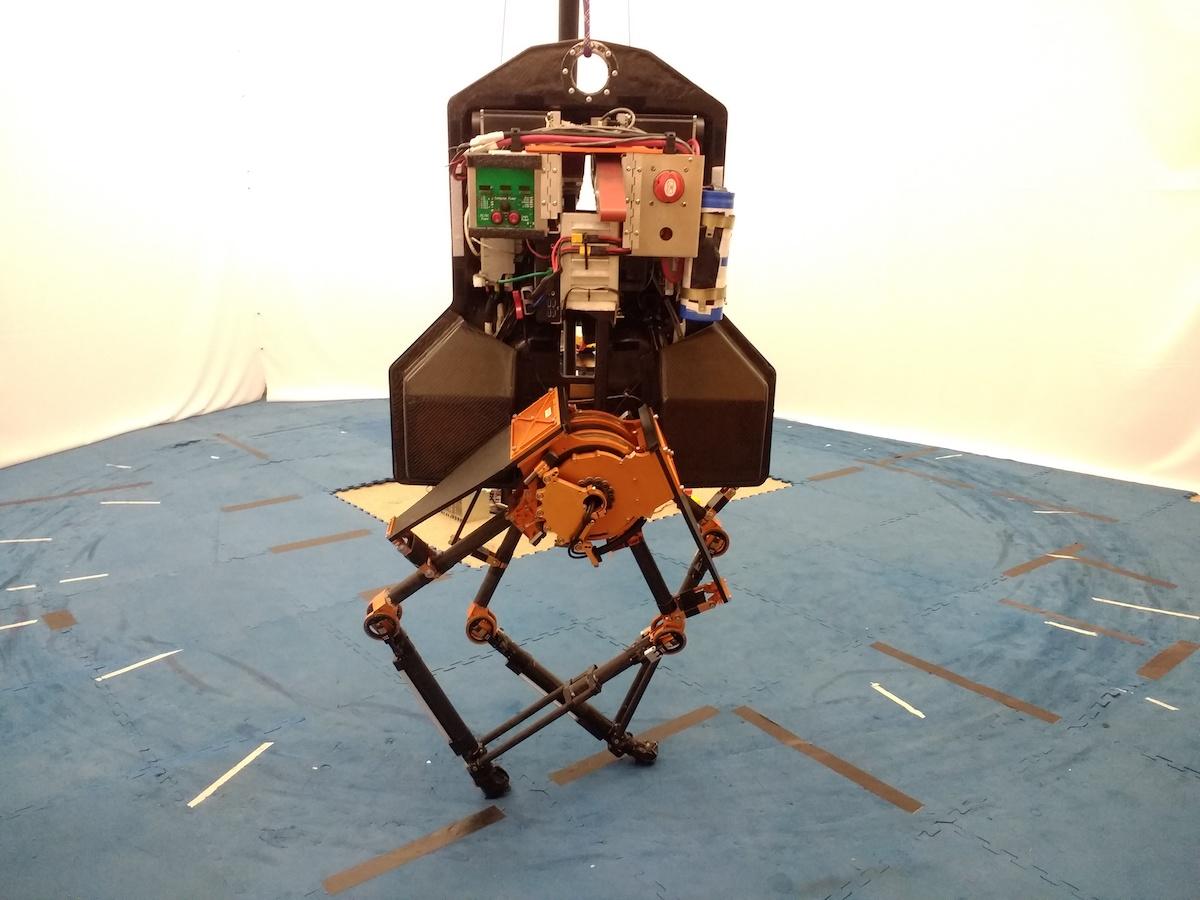
\includegraphics[width = 0.4\textwidth]{img/atrias1.jpg}
    %\includegraphics[width = 0.35\textwidth]{img/atrias2.jpg}
    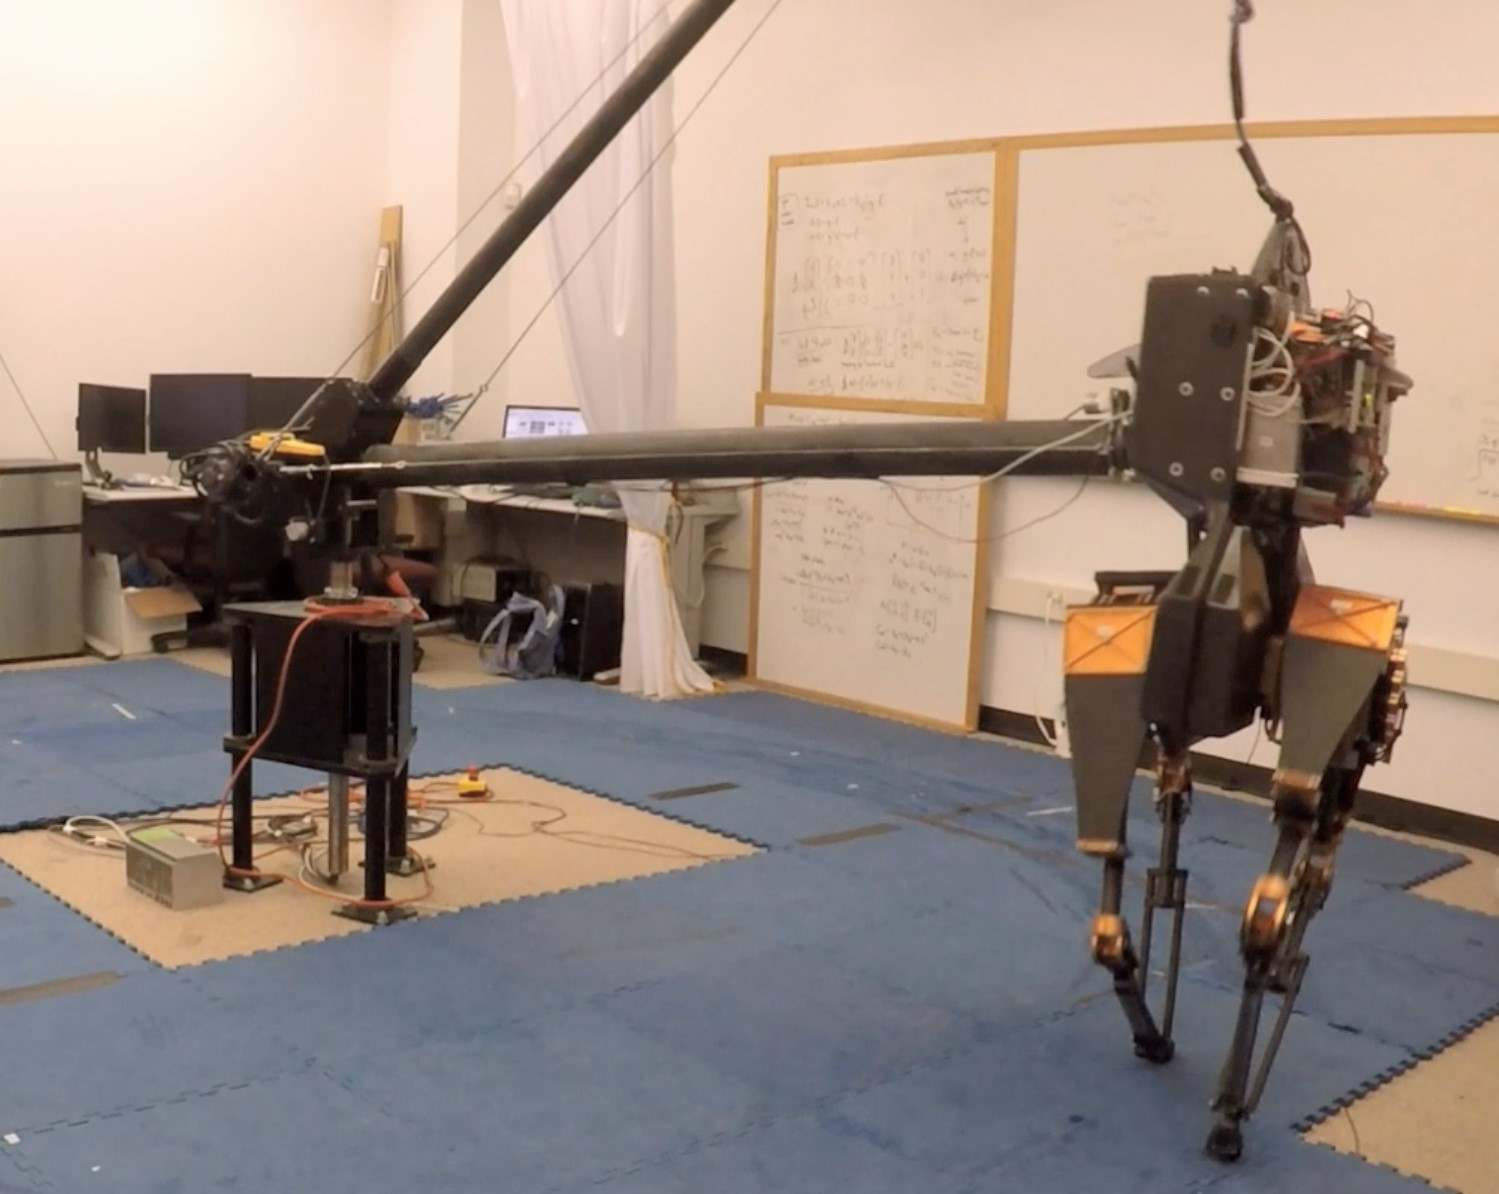
\includegraphics[width = 0.4\textwidth]{img/atrias_dog5d_walking_around_boom.jpg}
    \caption{\small{Our testbed is CMU's ATRIAS robot. 
    %While ATRIAS can walk in 3D, our experiments are focused on walking around a boom.
    }}
        \vspace{-5mm}
    \label{fig:atrias}
\end{figure}
%In our previous work, we proposed a transformation based on domain knowledge that reparameterized human-like walking controllers based on their behaviour in a high-fidelity simulation.
%The main idea was that some behavioural cues have a higher probability of transferring between simulation and hardware than exact cost or controller performance. For example, a controller that falls instantly in simulation by tilting its torso, would have a small chance of walking on hardware. On the other hand, a controller that walks efficiently in simulation might have a higher chance of walking on hardware, albeit with a different cost. Hence, it makes sense to roughly group parameters based on the behaviour they produce in simulation, and use this as a distance metric to distinguish between them. 

One way of incorporating domain knowledge could be to learn approximate models of the system from simulation, before moving to hardware. The idea of using simulation performance to speed up optimization on hardware has been explored before. A common approach is to learn controllers in simulation, and use this as a starting point on hardware. A domain expert would then typically have to fine-tune parameters on hardware. \cite{mordatch2015ensemble}~learn parameters using a collection of simulations that help account for model uncertainty. \cite{ha2015reducing}~iteratively learns both the model and controller parameters using the differences between simulated behaviors and observed hardware experiments. 
%\AR{Add work on developing transition models, model-based stuff here}
 \cite{marco2017virtual}~uses evaluations from simulation as a noisy prior for the optimization on hardware. \cite{cully2015robots}~pre-selects high performing controllers from simulation and search among them on hardware. 
 
\section{Adding prior knowledge to optimization}

 \textbf{We propose incorporating domain knowledge by building informed feature transforms that project the higher dimensional controller parameter space to an easy to optimize lower dimensional space of features.} These can be expert-designed or learned from data, as described below:
 
 \subsection{Expert-designed feature transforms}
 We use human-walking inspired features to develop a feature transform for bipedal walking that roughly groups controllers based on their walking features in short simulations. The objective of such a transformation is that some behavioural cues have a higher probability of transferring between simulation and hardware than exact cost or controller performance. For example, a controller that falls instantly in simulation by tilting its torso, would have a small chance of walking on hardware. On the other hand, a controller that walks efficiently in simulation might have a higher chance of walking on hardware, albeit with a different cost. Hence, it seems reasonable to roughly group parameters based on the behaviour they produce in simulation, and use this as a distance metric to distinguish between them. Despite being motivated by human walking features, these features also generalize to other robot morphologies and controllers, like the ATRIAS biped. 
 \subsection{Data-driven feature transforms}
Using extensive expert knowledge, as suggested above, has several advantages. It helps us learn and design features fast as well as provides transparency as to what the learning approach is prioritizing. However, it does raise concerns about problems for which such knowledge might not be available or as easily implementable. With this in mind, \textbf{we also develop a method to construct an informed metric automatically, without relying heavily on domain experts}. We propose to learn a distance metric with a neural network, utilizing data obtained from a high-fidelity simulator. This involves first running short simulations of a locomotion controller on a large grid of control parameters and recording the behavior of each set of parameters. The neural network then learns a mapping between input controller parameters and simulation output/behavior. We propose two ways of defining the target to be learned by the network. The first approach is based on the cost function that is to be optimized with BO on hardware, or a perturbed simulator. The second is cost-agnostic: learning to reconstruct a summary of robot trajectories obtained from simulation. This provides a useful re-parameterization: controller parameters that produce similar walking trajectory summaries are closer in this re-parameterized space. 
 
% Shall we name the controllers in the introduction: reactive and neuromuscular? Or is this to much detail for intro?

\section{Accounting for mismatch between hardware and simulation}
 An important question that arises when using simulation to guide hardware searches is: how can we learn and take into account the differences between simulation and hardware? For example \cite{macalpine2016adaptation} adapts the target task based on the mismatch between the expected and actual performance. \cite{marco2017virtual} develops an automatic way of transitioning between simulation and hardware based on data collected so far. 
 
 \textbf{We propose to learn a mismatch-map that represents the mismatch between behaviour encountered in simulation and hardware.} This allows us to build an error map over our parameter space, based on data. We start by trusting all simulation points with predicted mismatch of 0, and as we sample points on hardware, we update our estimate of error on each simulation sample. The advantage of this is that we can have different error values for different regions of parameter space, as some parts of the parameter space might transfer well between hardware and simulation, while others might not. %Using this trust-map, we can achieve significant sample-efficiency even with significantly perturbed simulations. %This is a promising result that is being tested on hardware.
To study the efficacy of this approach, we create a series of increasingly approximate simulators and use features from approximate simulators to optimize controllers on the original simulator. This allows us to empirically examine the deterioration of sample-efficiency as the simulator becomes more and more inaccurate, as well as the advantage of building a mismatch-map to close the loop between simulation and hardware. Our experiments show that this approach can learn controllers when simulation dynamics are perturbed by up to 60\% of their ``true" value. In addition, it is also robust to systematic under-modelling errors, such as unmodelled joint friction, actuator dynamics and other robot components. In comparison, other approaches from the literature that use simulation to speed up hardware experiments, such as \cite{cully2015robots}, suffer when simulation is significantly different from hardware. 

\AR{TODO : Implement 50d with mismatch on hardware}

\section{Using neural networks to learn walking policies}

While expert-designed policies are extremely powerful tools for sample-efficiency as well as safety of the robot, it can be challenging to design them in some situations. In such cases, high-dimensional policies like neural networks can be very useful. Typically, these are trained in simulation with deep reinforcement learning, and are shown to be capable of generating very diverse sets of behaviours. For example, \cite{silver2016mastering} use deep reinforcement learning to solve compledx long horizon games like AlphaGo, starting with no human input. Similar progress has been achieved in the domain of continuous control, dealing with very high dimensional state and action spaces. For example, Deep Deterministic Policy Gradients (DDPG) ~\cite{lillicrap2015continuous} and Trust Region Policy Optimization  (TRPO) ~\cite{schulman2015trust} can solve several control challenges in the Mujoco simulation environment \cite{todorov2012mujoco}. %\cite{heess2017emergence} show that a variant of the Proximal Policy Optimization (PPO) \cite{schulman2017proximal} can learn to control a very high degree of freedom humanoid robot in Mujoco, even in very challenging environments. Similarly, \cite{rajeswaran2017towards} use a variant of DDPG to learn to do dexterous manipulation with a high degree of freedom hand in simulation.

While simulation results for deep RL are very impressive, the simulation-hardware gap makes most controllers learned in simulation unsuitable to be implemented on hardware. This is partly because simulations are not perfect representations of real systems, but also because learning approaches often tend to exploit simulation inaccuracies to achieve better performance. 
%Recent work learns parameters of expert controllers on hardware sample-efficiently, for example \cite{antonova2017deep} and \cite{cully2015robots} use Bayesian Optimization. While these are promising, and robust even to hardware damage, they are limited by the controllers they can represent. On the other hand, high-dimensional neural network policies can approximate arbitrarily complex controllers, but too expensive to optimize on hardware. 
One approach to learn policies in simulation and deploy on hardware is domain randomization \cite{mordatch2015ensemble}. It can be used to learn robust neural network policies in simulation by applying random perturbations to the dynamics and other properties of the simulator. This approach has been applied to manipulation problems \cite{peng2017sim}, as well as quadrupedal locomotion problems \cite{tan2018sim}. However, typical domain randomization can lead to controllers that perform worse than controllers trained without randomization \citep{tan2018sim}, as well as make the learning problem much harder \citep{2018arXiv180800177O} taking over 100 years of simulation time to learn successful policies.   

 Domain randomization from scratch is especially challenging for under-actuated bipedal robots, as the basin of stability around a controller is typically very small. As a result, it is very difficult to randomly explore the space of controllers to find successful controllers that stabilize a wide range of dynamic models, and other disturbances. Moreover, the learned controllers would typically be quasi-static in nature, similar to \cite{mordatch2015ensemble} in behavior, which is not very impressive in performance. 
 
We experiment with classical deep reinforcement learning techniques to learn robust controllers in simulation and test them on hardware. Instead of using domain randomization, we create disturbances in simulation by simulating ground height disturbances and study the effect of policy structure on the rate of transfer. Starting with a high-fidelity simulator \citep{martin2015robust}, we experiment with different controller structures, and study their effect on transfer from simulation to hardware, without any domain randomization. The first neural network policy is a general policy that directly outputs the desired actions of the robot, while the second has the structure of an expert-designed policy and predicts the desired states for this policy. We find that structured neural network controllers have a fast training rate in simulation as well as higher rate of transfer to hardware. The structure also gives the user the power to modify the controller, if required, without having to re-train the neural network from scratch.


%Using our feature transform, we incorporate domain knowledge in BO, and optimize three walking controllers on ATRIAS - two on hardware and all three in simulation. BO equipped with domain knowledge is found to be much more sample-efficient than traditional BO. Using our trust-map, we can further improve sample-efficiency in perturbed simulation experiments. This is a promising result that needs to be tested on hardware in the future.
\section{Summary of completed goals and contributions}

In work done, we present evaluations of our proposed methods on the ATRIAS biped robot (Figure \ref{fig:atrias}), ATRIAS simulation, and a 7-link biped simulation. 

First, we use expert designed controllers and optimize their parameters using BO. We evaluate different feature transforms on three  controllers of increasing dimensionality. We start with a 5 dimensional feedback-based reactively stepping controller, and increase its dimensionality to 9. Then we take a 50-dimensional highly non-linear neuromuscular controller and optimize its parameters. We successfully optimize parameters for a 5-dimensional and 9-dimensional controller on the ATRIAS hardware in less than 10 trials, which proves to be challenging for traditional BO. Our results show that these feature transforms - hand-designed and data-driven, extract useful information from simulations, and leads to an effective transfer of knowledge to hardware. 
%This motivates future work for using our approach on hardware for the 50-dimensional controller.

While, Bayesian Optimization benefits from feature transforms and informed distance metrics, we also explore if simulation can be useful in learning other walking policies which might be much higher dimensional. We train two neural network policies - with and without structure and study their rate of transfer to hardware. Our studies show that structured neural network policies have a higher rate of transfer between simulation and hardware as compared to unstructured neural network polices.

The main contributions of this thesis are as below:
\begin{itemize}
    \item A simulation-based feature transform that enables faster optimization of bipedal walking controllers on hardware.
    \item A hybrid optimization approach that integrates model-based information from simulation into a model-free global search framework like Bayesian Optimization
    \item A novel way of updating models from hardware data using feature transforms evaluated on simulation and hardware
    \item A study of the effect of structure on neural network policies trained in simulation and their rate of transfer to hardware
\end{itemize}
%The rest of the paper is organized as follows: In Section \ref{sec:background} we present background on the concepts used in this paper and summarize related work. In Section \ref{sec:dog} we describe our approach of using a locomotion feature transform in detail. Section \ref{sec:atrias_cont} describes our test platform ATRIAS and the controllers used in our experiments. In Section \ref{sec:experiments} we describe our simulation and hardware experiments. Section \ref{sec:conclusions} concludes with further discussion.

\chapter{Background}
\label{chap:back}

In this Chapter, we will review the use of reinforcement learning and Bayesian optimization in robotics, using simulation information to learn faster on hardware and learning the mismatch between the dynamics in simulation and hardware. We also give a short introduction of other policy search methods in literature, which might benefit from simulation information.


\section{Reinforcement Learning}
\label{sec:dp}

Let us consider a controller (agent) that interacts with a process (environment) through a action, which changes the state of the process and generates a reward (feedback from the environment) (Figure \ref{fig:rl}). The controller observes the new state and the reward, and the whole process repeats. The behaviour of the controller is determined by a policy that maps the process state to an action. The process follows a stochastic or deterministic dynamics model which determines how the state changes as a result of actions. 

\begin{figure}[t]
    \centering
    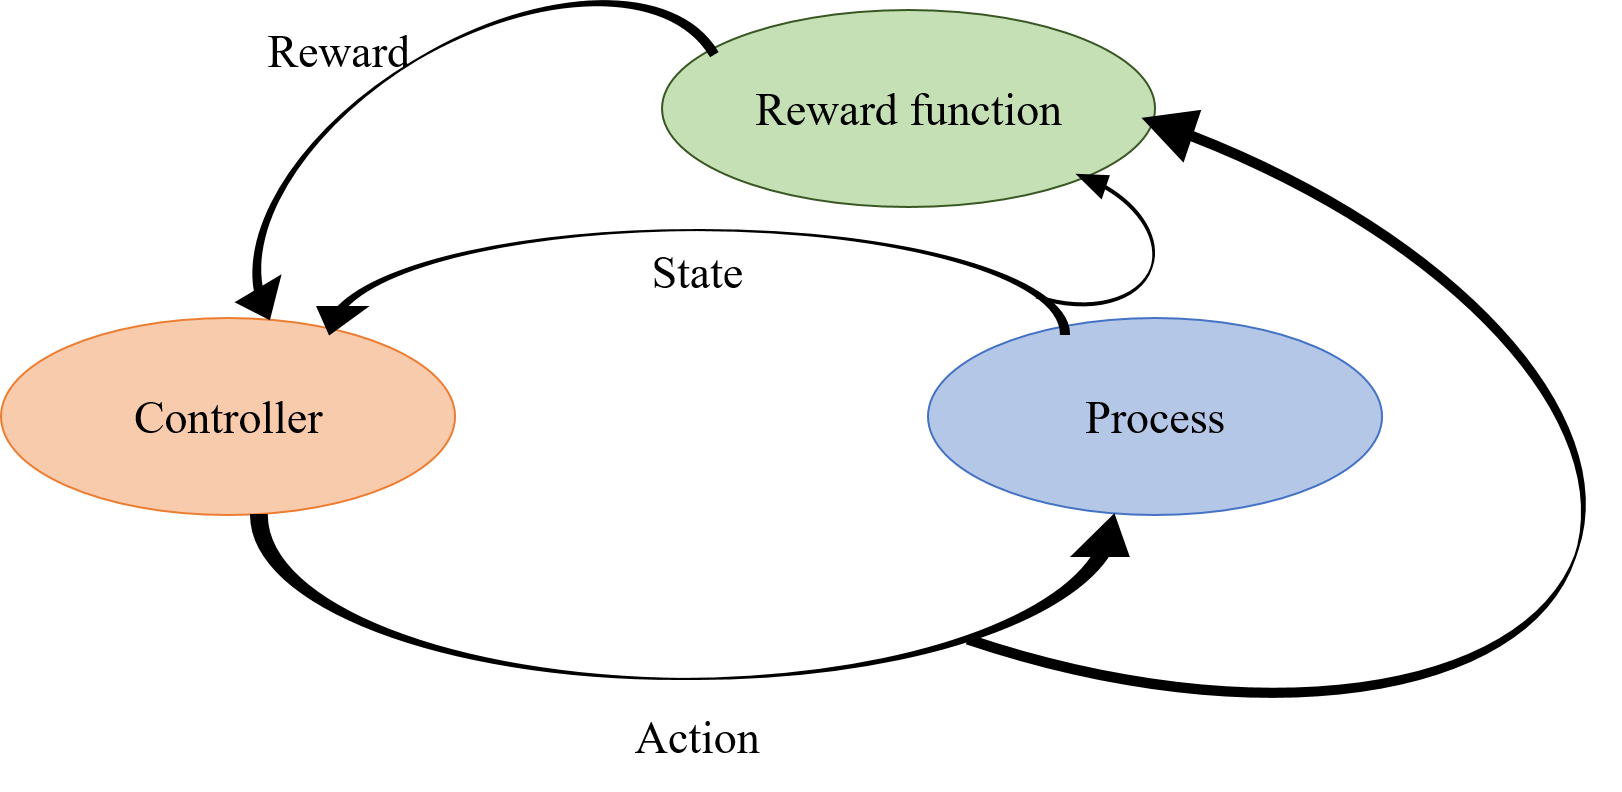
\includegraphics[width=0.7\textwidth]{img/reinforcementLearning.png}
    \caption{The interaction between the controller, process and reward function in dynamic programming and reinforcement learning.}
    \label{fig:rl}
\end{figure}

The goal of reinforcement learning is to find an optimal policy that maximizes the (expected) return, consisting of the (expected) cumulative reward over the course of this interaction, called the value function. This framework can be used to address problems from a variety of fields, e.g., automatic control, artificial intelligence, operations research, and economics.

%\AR{Add RL/DP equations from a standard reference to get notations right}
We assume a discrete-time process and denote the
current time step by $k$. The transition model $p$ is given by a probability distribution conditioned on the current state and current action. We assume a Markov decision process, where the distribution over the next state only depends on the previous state and actions.
\begin{equation}
    s_{k+1} \sim p(s_{k+1}|s_k,u_k)
\end{equation}
where $u_k \in \R^M$ denotes the current action, and $s_k, s_{k+1} \in \R^N$
denote the current and the next state respectively. We furthermore
assume that actions are generated by a policy
\begin{equation}
    u_k \sim \pi_{\theta}(u_k|s_k)
\end{equation}
which is modeled as a probability distribution conditioned on the current state. This lets us naturally include exploratory actions in the policy. The policy is parameterized by some policy parameters $\theta \in \R^M$. Over one episode, the sequence of states and actions forms a trajectory, denoted by $\xi = [s_{0:H}, u_{0:H}]$ where H
denotes the length of the episode. At each instant of time,
the learning system receives a reward (or cost for minimization) denoted by $r(s_k, u_k) \in \R$.

The objective of policy search algorithms is to maximize the expected return of a trajectory, as a function of the policy parameters $\theta$. We assume no-discounting in all our formulations, but discounting factors that weigh future costs lower than the current cost could be added.

\begin{equation}
    J(\theta) = \mathds{E}[\sum_{k=0}^H r_k]
\end{equation}

In general, for each considered policy $\pi_{\theta}$ , a
state-value function $V_\pi(s)$, and a state-action value function (Q-function) $Q_\pi(s,u)$ can be defined as
\begin{align}
    V_\pi(s) = \mathds{E}[\sum_{i=k}^H r_i | s_k = s] \\
    Q_\pi(s, u) = \mathds{E}[\sum_{i=k}^H r_i | s_k = s, u_k = u]
\end{align}
Note, that we can define the expected return in terms of the state-value
function by
\begin{equation}
    J(\theta) = \int_s p(s_0)V_\pi(s_0) ds_0
\end{equation}
where $p(s_0)$ is the probability of $s_0$ being the initial state of an episode.

In the presence of a model, one of the widely used optimal control methods in robotics are dynamic programming algorithms, which can be considered a part of reinforcement learning. Popular dynamic programming methods include value iteration or policy iteration, which are iterative methods that are guaranteed to converge to the global optimum \citep{bertsekas1995neuro}. However, dynamic programming methods do not scale to higher dimensional problems, leading to a ``curse of dimensionality". For example, value iteration converges to the true value function in polynomial time in the number of states and actions \citep{sutton1998reinforcement}. This raises concerns about generalizing to higher dimensions, and especially for continuous action and states. To deal with this, approximate dynamic programming approaches have been suggested, for example, \cite{atkeson2007randomly} randomly sample over actions in a continuous space to avoid discretizing actions. \cite{whitman2009control} break down the problem of controlling a 5-link biped into  4 simpler, lower-dimensional problems and solve each separately. 

Alternatively, in the absence of a model, function approximators can be used to learn the value function and Q-function, resulting in feasible methods even for higher dimensions and continuous action states, example SARSA and Q-learning  \citep{busoniu2010reinforcement}. However, this can result in biases in the estimate of the value function, especially with limited data. Unfortunately, in the general case, since these methods depend on their previous estimate of the target to generate the next solutions, they have an inherent bias based on their initial estimate. Coming up with an appropriate function approximator is a non-trivial problem and can involve using prior knowledge that might not be available, especially for model-free RL. Despite its short-comings, function approximators like deep neural networks have been shown to produce very impressive results in high dimensional control problems. We will talk more about these in Section \ref{sec:deepRL}

Policy search methods avoid the problem of approximating the value function or the Q-function by directly searching for an optimal control policy that maximizes the expected return. For a general problem, the optimization criterion may be a non-differentiable function, with multiple local optima. This means that global, gradient-free optimization techniques are more appropriate than local, gradient-based techniques. Some successful techniques include covariance-matrix adaptation \citep{hansen2006cma}, Bayesian optimization \citep{BOtutorial2016} and cross-entropy optimization \citep{rubinstein1999cross}. We primarily use Bayesian optimization in this work, and we describe that next.
%\AR{Mention a few more policy search works like PILCO, reinforce, etc.}

\section{Bayesian Optimization for Robotics}

In this section, we will provide a basic introduction of Bayesian optimization (BO) and Gaussian processes. This will be followed by a survey of BO for policy search in robotics and in particular, using BO with trajectory information.

\subsection{Bayesian Optimization and Gaussian Processes}
Bayesian optimization (BO) is a framework for sample-efficient black-box and gradient free global search. It was introduced by \cite{jones1998} and originally was referred to as Efficient Global Optimization. 
Recent tutorials like  ~\cite{BOtutorial2016} and ~\cite{BOtutorial2010} provide a  comprehensive overview. Here, we will summarize the basic background for Bayesian optimization to establish notation that will be used in the following sections.

The goal of BO is to find $\pmb{x}^*$ that optimizes an objective function $f(\pmb{x})$, while executing as few evaluations of $f$ as possible. 
The class of functions is not restricted to continuous or smooth functions and hence BO can optimize non-differentiable functions. Little or no a-priori knowledge about $f$ is necessary, but if available, prior knowledge can be incorporated (as we will discuss shortly).

The optimization starts with a prior roughly capturing the prior uncertainty over the value of $f(\pmb{x})$ for each $\pmb{x}$ in the domain. If no prior knowledge is available, this prior can be uninformed and updated with data. As points are sampled, these are included into the estimate of $f(\pmb{x})$, giving an approximate model based on data seen so far. An auxiliary optimization function, called the \textit{acquisition function}, is used to sequentially select points  $\pmb{x}_n$ to sample next, based on the current model of $f(\pmb{x})$. $f(\pmb{x}_n)$ is then evaluated and added to the sampled points. The aim of the acquisition function is to automatically balance exploration and exploitation: select points for which the posterior estimate of the objective $f$ is promising, while also decreasing the uncertainty about $f$. An example of BO is shown in Figure \ref{fig_bo_illustration}. 

\begin{figure}[t]
\centering
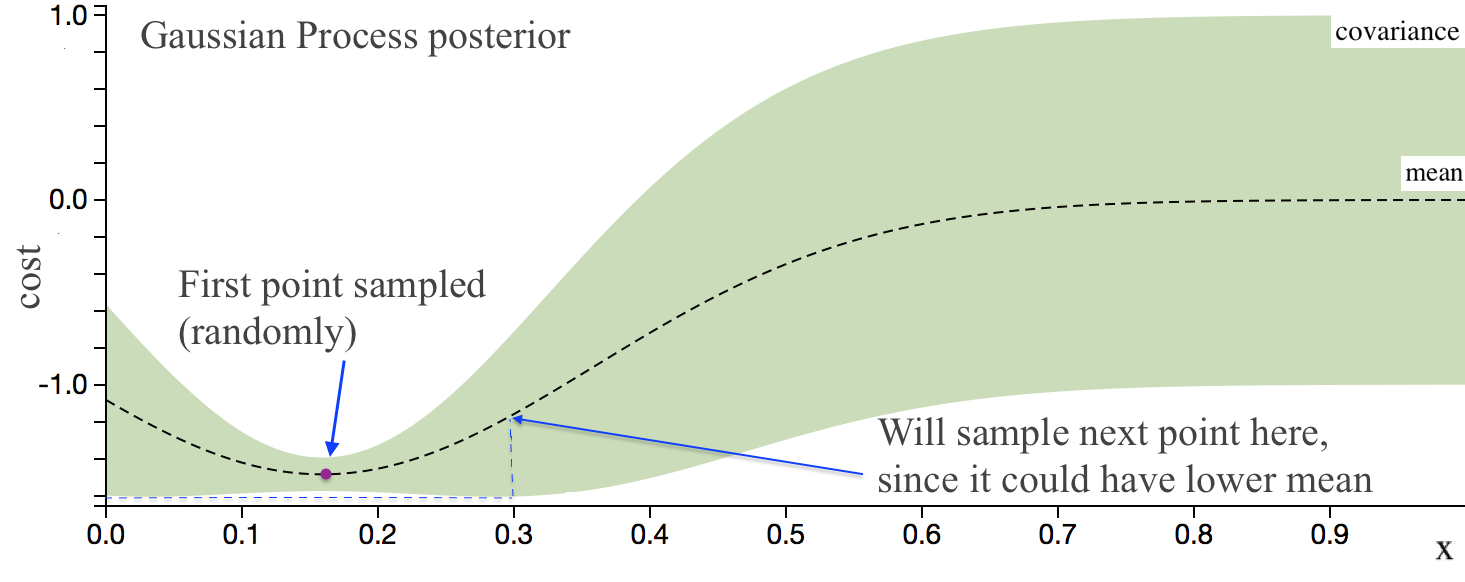
\includegraphics[width=0.75\textwidth]{img/bo_first_point.png}
\vspace{4px}
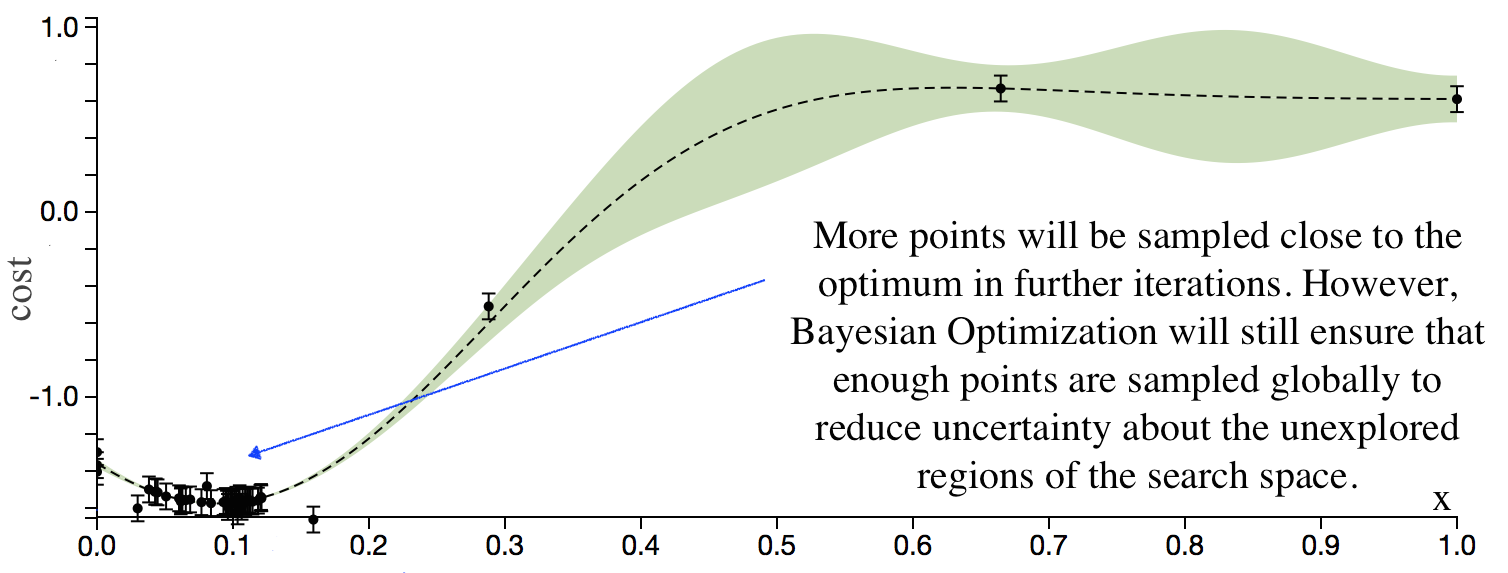
\includegraphics[width=0.75\textwidth]{img/bo_later_points.png}
\caption{\small{Bayesian Optimization posterior for a 1D function. Acquisition function computes the location of points to sample, taking into account both estimated mean and variance (uncertainty).}}
\label{fig_bo_illustration}
\end{figure}

Expected Improvement (EI) function is commonly used as an acquisition function. EI selects $\pmb{x}$ to maximize expected improvement over the value of the best result obtained so far ~\citep{mockus1978ei}. For maximization problems:
\begin{align}
&EI(\pmb{x}) =
\begin{cases}
\big[f(\pmb{x}^+) \!-\! \mu(\pmb{x})\big] \Phi(Z) + \sigma(\pmb{x}) \phi(Z) & \text{if } \sigma(\pmb{x})\!>\!0 \\
0 & \text{ otherwise}
\end{cases} 
\end{align}
where $ \pmb{x}^+ = \argmax_{x_i \in x_{1:t}} f(\pmb{x}_i) $, $\quad Z = (f(\pmb{x}^+) \!-\! \mu(\pmb{x})) / \sigma(\pmb{x})$. 

$\pmb{x}_i$ are points for which objective $f$ has been evaluated so far, $\mu,\sigma$ are posterior mean, variance; $\phi, \Phi$ are PDF and CDF of standard normal distribution. In all our experiments, we use EI as the acquisition function, as it doesn't have any hyperparameters to tune.

Another frequently used acquisition function is Upper Confidence Bound (UCB) or, for minimization problems, Lower Confidence Bound (LCB)~\citep{srinivas2009gpucb}. LCB balances the mean $\mu$ and variance $\sigma$ of the posterior by selecting points which minimize 
\begin{equation}
\label{eq:lcb}
    LCB(\pmb{x}) = \mu(\pmb{x}) - \alpha \sigma(\pmb{x})
\end{equation}

While there can be many ways of modelling $f(\pmb{x})$, we describe a specific non-parametric way of describing $f(\pmb{x})$ using a Gaussian Process (GP). A Gaussian Process is defined by a set of random variables that are jointly Gaussian. It can be completely specified by its mean function and covariance function. 
\begin{align}
f(\pmb{x}) \sim \mathcal{GP}(\mu(\pmb{x}), k(\pmb{x}_i, \pmb{x}_j)),
\end{align}
with mean function $\mu(\pmb{x})$ and kernel $k(\pmb{x}_i, \pmb{x}_j))$. 
\begin{align}
   \mu(\pmb{x}) = \mathds{E}[\pmb{x}] \\
   k(\pmb{x}_i, \pmb{x}_j)) = \mathds{E}[(f(\pmb{x}_i)-\mu(\pmb{x}_i))(f(\pmb{x}_j)-\mu(\pmb{x}_j))]
\end{align}
 %This means that $(f(\pmb{x_1}), f(\pmb{x_2})) \sim \mathcal{N}(\pmb{\mu}, \Sigma)$. To maintain consistency, the marginal distributions are also required to be Gaussian, ie, $f(\pmb{x_1}) \sim \mathcal{N}(\mu_1, \Sigma_{11})$.  Notice that the consistency requirement is automatically fulfilled if the covariance function specifies entries of the covariance matrix.

Assuming Gaussian noise with variance $\sigma^2_{noise}$ on our measurements $y_i$, 
\begin{equation}
    \pmb{y}_i = f(\pmb{x}_i) + \epsilon_{\mathcal{N}(0, \sigma^2_{noise})}
\end{equation}
Gaussian Process conditioned on sampled points represents a posterior distribution for $f$. After evaluating $f$ at points $x_1,...,x_t$ the predictive posterior $P(f_{t+1} | \pmb{x}_{1:t}, \pmb{y}, \pmb{x}_{t+1}) \sim \mathcal{N}\big(\mu_t(\pmb{x}_{t+1}), cov_t(\pmb{x}_{t+1})\big)$ can be computed in closed form with mean and covariance:
\begin{align}
\mu_t(\pmb{x}_{t+1}) = \pmb{k}^T [\pmb{K} + \sigma^2_{noise} \pmb{I}]^{-1} \pmb{y} \quad \quad \quad \\
cov_t(\pmb{x}_{t+1}) = k(\pmb{x}_{t+1}, \pmb{x}_{t+1}) - \pmb{k}^T [\pmb{K} + \sigma^2_{noise} \pmb{I}]^{-1} \pmb{k},
\end{align}
where $\pmb{k} \in \R^t$, with $\pmb{k}_i=k(\pmb{x}_{t+1}, \pmb{x}_i)$; $\pmb{K} \in \R^{t \times t}$ with $\pmb{K}_{ij} = k(\pmb{x}_i, \pmb{x}_j)$; $\pmb{I}$ is an identity $\in \R^{t \times t}$, and $\pmb{y}$ is a vector of values obtained after evaluating $f(\pmb{x}_1), ..., f(\pmb{x}_t)$. More details can be found in~\cite{GPsMLBook}.

The prior mean function $\mu(\pmb{x})$ can be set to $0$ if no relevant domain-specific information is available. The kernel $k(\pmb{x}_i, \pmb{x}_j)$ encodes how similar $f$ is expected to be for two inputs $\pmb{x}_i, \pmb{x}_j$. 
The value of $f(\pmb{x}_i$) has a significant influence on the posterior value of $f(\pmb{x}_j)$, if $k(\pmb{x}_i, \pmb{x}_j)$ is large. The Squared Exponential (SE) kernel is a commonly used similarity metric:
\begin{equation}
k_{SE}(\pmb{x}_i, \pmb{x}_j) = \sigma_k^2 \exp\Big(- \frac{1}{2 \pmb{l}^2} \|\pmb{x}_i - \pmb{x}_j\|^2 \Big),
\end{equation}
where $\sigma_k^2, \ \pmb{l}^2$ denote signal variance and a vector of length scales respectively; $\sigma_k^2, \ \pmb{l}^2$ are called `hyperparameters' in BO literature. It is possible to adjust these automatically during optimization to learn the overall signal variance and how quickly $f$ varies in each input dimension. %Squared Exponential kernel is a special case of a more general class of Mat\'ern kernels~\citep{stein1999interpolation}.


\subsection{Bayesian optimization for policy search}
 As described in Section \ref{sec:dp} policy search circumvents the need to approximate value functions by directly searching for policies that maximize the expected return $J(\theta)$.
 \begin{equation}
    J(\theta) = \mathds{E}[\sum_{k=0}^H r_k]
\end{equation}
The optimal policy parameters $\theta^*$ are defined as
\begin{equation}
    \theta^* = \argmax J(\theta)
\end{equation}

This optimization can be solved sample-efficiently using Bayesian optimization. In this setting, the parameters $\mathbf{x} = \theta$ and the reward/cost function $f = J$. BO samples different policy parameters, executes the policy, and obtains the reward of the episode. This is then used to update the model of $f$ and used to choose the next policy to sample using the acquisition function. It is worth noting that while usually function approximators in reinforcement learning are over states, BO is building an approximation over policies. This way, it is directly searching for the optimal policy that leads to the maximum reward with a fixed initial state distribution. This circumvents building a model over the whole state space, but depends on a specific initial condition distribution. %However, as explained before, such assumptions are common in policy search literature.


\subsection{Bayesian optimization for legged robots}

Bayesian optimization has been used in robotics, usually to tune parameters of controllers, cost functions or planners. The advantage of using a global search framework like BO is that globally optimal policies can be discovered. These may perform better than human hand-designed policies as well as locally optimal solutions. As shown in~\cite{englert2016combined}, the alternative of using Reinforcement Learning (RL) algorithms for policy search might not discover global optima reliably. \cite{frean2008using} use BO to optimize parameters of a neural network controller for a two-link pendulum on a cart. \cite{marco2017virtual} solve the problem of balancing a pole on a real inverted pendulum, by optimizing the cost function for a LQR controller. Authors also propose a way of trading-off simulation and hardware experiments to optimally switch between hardware and simulation for experiments. \cite{martinez2007active} learn the policy for planning the path of a simulated robot that minimizes the uncertainty in its environment.

The most prominent works using Bayesian Optimization for locomotion controllers include \cite{lizotte2007automatic}, \cite{tesch}, \cite{cully2015robots} and \cite{calandra17thesis}. These works typically involve simpler to control robots or smaller bipeds than ATRIAS. \cite{lizotte2007automatic} use AIBO quadrupeds, \cite{tesch} use snake robots, \cite{cully2015robots} use hexapods and \cite{calandra2016bayesian} use a small biped.  \cite{tesch} optimize 3 parameters for a open-loop parametric controller that generates trajectories for a 16 degree of freedom snake robot. The generated solutions find fast moving gaits of about $0.13m/s$ in about 10-40 trials, depending on the difficulty of the task. Such performance was hard to achieve with hand-tuned parameters. \cite{lizotte2007automatic} use BO to optimize open-loop gait parameters for a AIBO robot to maximize velocity and smoothness of movement. They find that the Bayesian optimization
approach not only outperformed previous techniques, but used drastically
fewer evaluations.

%While quadrupeds, hexapods and snake robots can do dynamic gaits, the percentage of time spent dynamically is small as compared to the time spent statically stable. On the other hand, ATRIAS is a highly dynamic robot due to its point feet, and it cannot be statically stable, except in double-stance on a boom. This makes the optimization harder, as the system is unstable leading to discontinuities in cost functions.

\cite{calandra2016bayesian} use BO for optimizing gaits of a 4 dimensional controller on a small biped on a boom. They report needing 30-40 samples for finding walking gaits for a finite-state-machine based controller. This controller consists of 4 threshold parameters that switch the states of a finite-state-machine cycling between stance and swing for each leg. Optimizing a higher-dimensional controller, which is needed for more complex robots and tasks, might prove to be even more challenging. The learning could be especially difficult if a significant number of the points/parameters sampled would lead to unstable gaits and falls. Such samples might result in eventual wear and breakage of the robot hardware (even if care is taken to prevent actual falls). Hence, there is a need to either limit search spaces to ``safe" points, or bias the search towards such points. 

\cite{cully2015robots} tabulate best performing points in simulation versus their average score on a behavioural metric for a hexapod robot. This metric then guides BO to quickly find behaviours that can compensate for damage of the robot. The search on hardware is conducted in behaviour space, and limited to pre-selected ``successful" points from simulation.  This helps make their search faster and safer on hardware.   However, if an optimal point was not pre-selected,  BO cannot sample it during optimization, losing global optimality guarantees.  ``Best points" are cost-specific, so the map needs to be re-generated for new cost functions.

Our proposed method generalizes to highly dynamic behaviours and discontinuous cost functions, while maintaining the global guarantees of BO. We also bias our search towards sampling points successful in simulation (but not exclusively), leading to a sample-efficient and safer search.

\subsection{Incorporating behavior information in Bayesian Optimization}

Adding prior knowledge based on behavior of controllers is a promising avenue to speed up optimization. In higher dimensions, the performance of BO typically degrades, as discussed in \cite{localBO17}. Incorporating domain knowledge, in the form of behavior might speed up optimization in such cases.

Domain knowledge can be incorporated in the form of trajectory information. If we could query the resultant trajectory of each controller, the problem of optimizing the cost would be trivial, as can be expected. To elaborate, consider a Markov Decision Process starting from a state $s_0$, consisting of states $s$ and actions $u$, that follow a transition function $p(s_{k+1}|s,u)$ at time step $k$. Here $p$ defines the probability of transitioning to state $s_{k+1}$ given current state $s$ and taking action $u$. %A typical reinforcement learning problem is characterized reward function $R(x,u,x')$ and a policy $P_\pi(u|x,\theta)$ that maps states to actions,  given some parameters $\theta$. 
Bayesian Optimization, in the classic setting, studies episodic RL which looks at rewards at the end of the execution, or the value of a trajectory. Consider a trajectory $\xi = (s_0, u_0, \cdots , s_H, u_H)$. The probability of sampling this trajectory is
\begin{equation}
    P(\xi|\theta) = P(s_0) \prod_{k=0}^H P(s_{k+1}|s_k,u_k)P(u_k|x_k,\theta)
\end{equation}
The cumulative reward of a trajectory is given as
\begin{equation}
    R(\xi) = \sum_{k=0}^{H-1} R(s_{k+1}, u_{k}, x_{k})
\end{equation}
The expected return of a parameter set $\theta$ then becomes 
\begin{equation}
    J(\theta) = \int R(\xi) P(\xi|\theta) d\xi
\end{equation}

If we can query each trajectory $\xi$ for every controller $\theta$, the cost $J(\theta)$ is perfectly known and the uncertainty $\sigma$ is 0.

%The expected return could itself be a vector consisting of different aspects of a trajectory, for example, distance walked, average speed, cost of transport, etc. The overall cost is a combination of these:
\begin{equation}
    f(\theta) = J(\theta)^Tw
\end{equation}
where $w \sim \mathcal{N}(0, \Sigma_p)$.

%If we fit a GP to this linear setting, the mean and covariance functions become
\begin{align}
    E[f(\theta)] = J(\theta)\\
    E[f(\theta),f(\theta')] = J(\theta)^T \Sigma_p J(\theta)
\end{align}
%If $J(\theta)$ is a scalar, we can determine the the fitness or cost of each controller parameter uniquely in the second trial. 
The UCB acquisition for the posterior (similar to Equation \ref{eq:lcb}) is
\begin{align*}
    \mu(\theta) = J(\theta)\\
    \sigma(\theta) = k(x_2,x_2)-k(x_2,x_1)k(x_1,x_1)^{-1} k(x_1,x_2) = 0 \\
    UCB(\theta) = \mu(\theta) + \alpha \sigma(\theta) = J(\theta)^Tw \\
    \theta_{next} = \argmax_{\theta} UCB(\theta) = \argmax_{\theta} J(\theta)
\end{align*}
$\sigma(\theta) = 0$ is an intuitive result, as for a deterministic setting, there is no uncertainty about the posterior mean of any policy $\theta$. It is exactly equal to $J(\theta)$. Optimizing the acquisition function is equivalent to optimizing the cost. Although it can be difficult to optimize such a function globally, there is no real advantage to using Bayesian optimization anymore. Optimizing the acquisition function can typically need a very large number of samples, which are assumed to be much cheaper than evaluating a policy in BO. However, in the current case, sampling policies for optimizing the acquisition function is just as costly as sampling the actual cost. 
However, this is impossible for a system without unrolling every possible $\theta$ for a controller, which can be prohibitively large number of points. To overcome this, several alternative solutions to evaluating $J(\theta)$ for each point exist in literature.

\cite{wilson2014using} prove an upper bound on the expected improvement of polices as a function of trajectories induced by these policies. 
\begin{align}
%    |J(\theta_i) - J(\theta_j)| = |\int R(\xi)P(\xi | \theta_i) d\xi - \int R(\xi)P(\xi | \theta_j)| d\xi \\
%     = |\int R(\xi) (P(\xi | \theta_i) - P(\xi | \theta_j))| d\xi \\
%     \leq  \int | R(\xi) (P(\xi | \theta_i) - P(\xi | \theta_j))| d\xi \\
   |J(\theta_i) - J(\theta_j)|  \leq  Rmax \int | P(\xi | \theta_i) - P(\xi | \theta_j)| d\xi
\end{align}
The difference between expected returns is upper bunded by the maximum reward per trajectory $Rmax$, and the variational difference in trajectories induced by each policy. Using Pinsker's inequality, and using the fact that $|J(\theta_i) - J(\theta_j)| = |J(\theta_j) - J(\theta_i)|$  this can be written as
\begin{align}
    |J(\theta_i) - J(\theta_j)| = Rmax \sqrt{2} (\sqrt{KL(P(\xi|\theta_i)||P(\xi || \theta_j))} + \sqrt{KL(P(\xi|\theta_j)||P(\xi || \theta_i))} )
\end{align}

The authors use this symmetric positive definite result to construct a kernel defined as:
\begin{align}
D_{ij} = \sqrt{KL(P(\xi|\theta_i)||P(\xi || \theta_j))} + \sqrt{ KL(P(\xi|\theta_j)||P(\xi || \theta_i))} \\
K(\theta_i, \theta_j) = \exp(-\alpha * D_{ij})
\end{align}

This new Behavior Based Kernel (BBK) uses the KL distance of trajectories induced by the evaluated policies to calculate kernel distances. A kernel constructed to use behavior-based similarity offered an improvement over a standard SE kernel. However, BBK required obtaining trajectory data every time kernel values $k(\pmb{x}_i, \pmb{x}_j)$ were evaluated. This would not be tractable when optimizing locomotion controllers, as it would need a full evaluation to determine the kernel distance (similar to the problem we described above). The authors suggest combining BBK with a model-based approach to overcome this difficulty by learning a transition model for the problem. But building a reliable model might need several data points, and building good models with few data points is an interesting research question in itself.

\cite{cully2015robots} build a behavior map based on the simulation of controllers. They overcome the problem of building models of the robot from hardware data, but rely on behavior transfer between simulation and hardware. However, rather than using behavior as part of the kernel, as in \cite{wilson2014using}, they build a look-up map between behavior and ``successful" controllers. They then search in the low-dimensional behavior space, among the pre-selected controllers from simulation. Though this leads to a highly sample-efficient search and potentially safe samples, this method cannot search beyond the pre-selected points, and hence loses the global guarantees of BO.

\cite{marco2017design} design a kernel for LQR control assuming a quadratic cost and a one-dimensional linear system model. For such a problem, they show improvements in cost within 3 trials. It is unclear how this approach would scale to higher dimensional problems and other controllers.

Our approach constructs an informed kernel that incorporates behavior-based similarity, in a manner that ensures $k(\pmb{x}_i, \pmb{x}_j)$ can be obtained efficiently when running BO. We pre-calculate locomotion-specific features on a high-fidelity simulator by running short simulations, enabling us to efficiently calculate the kernel distances during optimization. Our feature transform also biases the search towards high performing points in simulation, which have a higher chance of being stable on hardware than randomly selected points. In this manner, we try to incorporate behavior information from simulation, as also was proposed in \cite{cully2015robots}, but maintain global guarantees of BO.



\section{Reinforcement learning for bipedal robots}
Reinforcement learning (RL) has been widely applied to robotics problems, including simulations and hardware of manipulation, locomotion, perception problems. The widespread use of RL makes it hard to review all works in robotics, hence we will focus largely on RL for bipedal locomotion. 

Some of the applications of RL on bipedal robots include, \cite{tedrake2004stochastic}, \cite{morimoto2005poincare}, \cite{benbrahim1997biped} and \cite{nakanishi2004learning}.
\cite{tedrake2004stochastic} started with a passively stable 3d biped and added ankle actuation. With simplifications, like decoupling the roll and sagittal degrees of freedom, they approximate a value function and the control policy using linear function approximators. This system was shown to learn to walk in a very short time. \cite{morimoto2005poincare} modulate the via-points of reference trajectories of hip and knee joints of a 5-link biped, by learning a value function, control policy and a Poincar\'e section of the robot. The policy-gradient method, aided by the Poincar\'e model, found robust walking solutions in 100 trials on a complex robot hardware. \cite{benbrahim1997biped} use a central-pattern generator (CPG) based controller, whose parameters are tuned online using an actor critic method. However, the robot had to be externally supported with a ``walker" to aid stability. \cite{nakanishi2004learning} use a rhythmic dynamic movement primitive to learn an initial gait from locomotion and adapt the frequency of oscillation using RL on a 5-link biped.

Another popular approach employing RL or DP in robotics is using it to learn the Center of Mass (CoM) trajectory, and follow it using optimization based Inverse Dynamics. \cite{kormushev2011bipedal} use RL to reduce the energy consumption by learning a variable-height CoM trajectory, with a evolving policy parametrization of their policy. The learned CoM trajectory exploits the passive dynamics of the COMAN robot and reduces the overall energy of walking better than the fixed policy parametrizations. \cite{feng2015optimization} use an approximation of dynamic programming, called Differential Dynamic Programming to optimize the CoM trajectory using an inverted pendulum model with ankle torques. Combining this with reactive foot placement in \cite{feng2016robust} results in very a robust walking controller on the ATLAS humanoid robot. An application of approximate dynamic programming for whole-body control of bipedal robots was described in \cite{whitman2009control}. \cite{whitman2009control} break down the problem of controlling a 5-link biped into  4 simpler, lower-dimensional problems - sagittal stance, sagittal swing, coronal stance and yaw control. The coupled dynamics of the simpler models are considered as disturbances. The control policy generated by dynamic programming is robust to perturbations in forward and lateral directions, as well as generalize to different speeds. This was also implemented on the Sarcos humanoid and shown to reject small unknown disturbances while walking.


%\cite{} use differential dynamic programming (DDP) to develop robust controllers applied to a 5-link biped. The differences between hardware and simulation are treated as disturbances that the learned feedback controller is able to reject.
%One of the common control parametrizations used with RL on bipedal robots are central pattern generators (CPGs). 

\subsection{Learning with neural networks in robotics}

Recently, there has been a surge in work using neural networks to control robots, though hardware results on locomotion robots are few. Techniques like deep reinforcement learning however have shown tremendous progress at solving complex manipulation and locomotion tasks in simulation. Recently deep reinforcement learning (DRL) has shown beyond human performance on complex long-horizon games such as Go \cite{silver2016mastering}, even when starting with no human input. Similar progress has been achieved in the domain of continuous control too, dealing with very high dimensional state and action spaces. For example, Deep Deterministic Policy Gradients (DDPG) ~\citep{lillicrap2015continuous} and Trust Region Policy Optimization  (TRPO) ~\citep{schulman2015trust} can solve several control challenges in the Mujoco simulation environment \citep{todorov2012mujoco}. \cite{heess2017emergence} show that a variant of the Proximal Policy Optimization (PPO) \citep{schulman2017proximal} can learn to control a very high degree of freedom humanoid robot in Mujoco, even in very challenging environments. Similarly, \cite{rajeswaran2017towards} use a variant of DDPG to learn to do dexterous manipulation with a high degree of freedom hand in simulation.

While simulation results for deep RL are very impressive, the simulation-hardware gap makes most controllers learned in simulation unsuitable to be implemented on hardware. This is partly because simulations are not perfect representations of real systems, but also because learning approaches often tend to exploit simulation inaccuracies to achieve better performance. High-dimensional neural network policies can approximate arbitrarily complex controllers, but too expensive to optimize directly on hardware. One approach to learn policies in simulation and deploy on hardware is domain randomization \citep{mordatch2015ensemble}. It can be used to learn robust neural network policies in simulation by applying random perturbations to the dynamics and other properties of the simulator. This approach has been applied to manipulation problems \citep{peng2017sim}, as well as quadrupedal locomotion problems \citep{tan2018sim}. However, typical domain randomization can lead to controllers that perform worse than controllers trained without randomization \citep{tan2018sim}, as well as make the learning problem much harder \citep{2018arXiv180800177O} taking over 100 years of simulation time to learn successful policies.   

\subsubsection{Deep Reinforcement Learning for locomotion}
\label{sec:deepRL}

\cite{peng2016terrain} formulate the problem of learning locomotion gaits as a actor-critic Reinforcement Learning with neural networks as function approximators for policy and value functions. The neural network takes as input terrain and robot states, parametrized leaps or steps as output. The input dimensionality is large (83D robot state and a 200D terrain state) and maps to a 29D control space, that operates at a high level, like leaps and steps for the robot, leading to about 570k parameter large network. The outputs from the policy network is fed to a finite state machine which is hand-designed to achieve the goal dictated by the neural network. While highly successful at traversing very uneven terrain, this network needs over 10 million data points to train the network. 
%Such approaches, however, are not data-efficient enough to support learning optimal parameters for locomotion controllers on real hardware. So in our work we are interested in combining sample efficiency of an approach like Bayesian Optimization with the flexibility and scalability of deep neural networks.

\cite{heess2017emergence} use deep reinforcement learning to learn locomotion tasks for a biped, humanoid walker and a quadruped, training the neural network with increasingly difficult terrains. The network takes as input the terrain state and the robot state and directly outputs the torques for each joint. They develop a robust policy gradient method that uses a trust region constraint to restrict the policy update from changing too much, making the policy gradient robust to noise and hyperparameter selection. This results in highly dynamic and robust gaits in simulation, though it is unclear if such policies can be learned on hardware.

To avoid having to learn such policies on hardware directly, \cite{tan2018sim} use domain randomization in simulation to learn robust policies for a quadrupedal robot. They learn two dynamic gaits - trotting and galloping in simulation, and test the trained policies on hardware. The trained policies were able to achieve about the same speed as handcrafted policies, they consumed less mechanical power. While controllers trained with domain randomization had a lower expected return in simulation than those trained without, their performance on hardware was much better. This is expected because robust controllers are typically more conservative, but easily generalizable to different systems.

%\AR{Maybe add a section about other sim to real work in deep rl}

\subsubsection{Guided policy search and related methods}

Guided policy search is a recently popularized method for learning policies for robotic tasks \citep{levine2013guided} using neural networks. It has been applied to learning policies from images for complex manipulation tasks, such as peg-in-hole \cite{levine2016end}, contact-rich tasks like opening doors \cite{levine2015learning}, etc. These networks represent global policies that are initialized by locally optimal policies. On facing new situations, where the local policies fail, a new local policy is initialized and trained to minimize cost and stay close to the global policy. The global policy is now updated to match the local policy. This ensures an increasingly general global policy that stays close to the initial policy, minimizing the ``forgetting" factor for neural networks. 

While there hasn't been work on locomotion on hardware with guided policy search, initializing the network in simulation over perturbed models and implementing on hardware seems straightforward. To enable fast learning on hardware, it might be beneficial to aid the policy gradients from optimal gradient step-size from simulation. This can be done either using natural gradients \cite{peters2006policy} from simulation or a meta-function that predicts gradient step-size \cite{meier2017online}. Aiding gradient descent based on information from simulation can help with sample-efficiency on hardware. This was originally proposed in \cite{abbeel2006using} where exact evaluations were aided with approximate gradients to suggest local improvements. While the exact value of the value function might be different between simulation and hardware, the gradient direction and step-size might have higher probability of transferring. Since learning rates are sensitive to hyper parameters like step-size, learning these in simulation seems straight-forward and beneficial. This can be done in combination with a mismatch-map which predicts the likelihood of transfer between simulation and hardware. If we expect high mismatch, we can use hardware samples to learn the correct learning rate. 
\chapter{Learning to learn}
\label{chap:learn}

Learning to learn or meta-learning is growing increasingly popular in machine learning and robotics. It can refer to learning hyper-parameters for learning methods to overcome the need for hand-tuning these, from simulation to hardware or across tasks. In our case, we use simulations to extract information that will enhance the rate of learning on hardware. %One could say that we are ``priming the pump" in simulation before moving on to hardware. 

In this chapter we describe two ways of adding data from simulation to hardware optimization. We start by describing feature transforms in simulation and using them to speed up learning on hardware. The second approach is to learn a robust policy directly in simulation and implementing it on hardware. The two approaches have different advantages. While learning features lets us use very inaccurate simulations, and still learn on hardware, it needs expert input in designing the controller structure. On the other hand, directly learned policies can have very small amount of expert input and still successfully learn walking controllers. Although, we show that adding structure in the form of expert knowledge can greatly help in the rate of transfer of learned policies between simulation and hardware.

We start by describing a hand-designed locomotion-specific feature transform which is inspired from the Determinants of Gait walking metric \citep{inman1953major}. Next, we explain an automatic way of learning a feature transform from data using neural networks. Both these approaches aim at collecting data by running a lot of simulations (``Big simulation") and use it to extract behavioral information about the controller space. This information will later be used for hardware and perturbed-simulation experiments that demonstrate sample-efficiency at learning controllers.

\section{Distance metrics from simulation}
In this section, we describe our proposed bipedal locomotion specific feature transform, followed by a more general transform learned from data. Once these feature transforms are collected for a range of controllers in simulation, they are then used in the optimization of controllers on hardware. The general pipeline of this approach is shown in Figure \ref{fig:approach}.

\begin{figure}
    \centering
    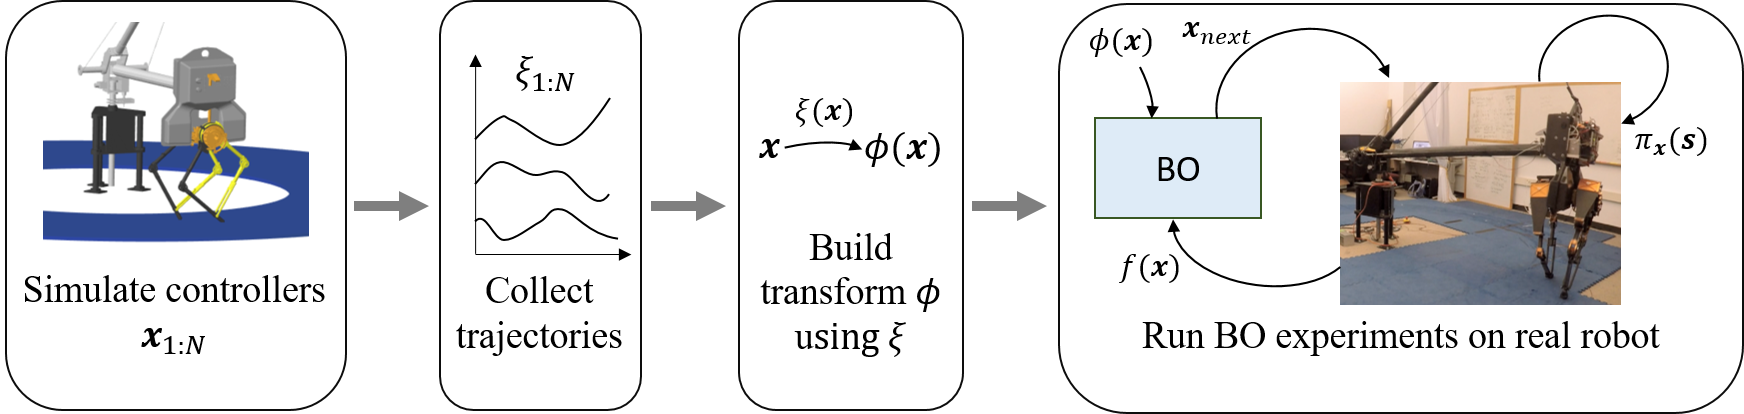
\includegraphics[width=0.9\textwidth]{img/approach.png}
    \caption{Overview of our proposed approach. Here, $\pi_{\pmb{x}}(\pmb{s})$ is the policy (described in Section~\ref{});  $\pmb{x}$ is a vector of controller parameters; $\pmb{s}$ is the state of the robot; $\xi(\pmb{x})$ is a trajectory observed in simulation for $\pmb{x}$; $\phi(\cdot)$ is the transform built using $\xi(\pmb{x})$. $f(\pmb{x})$ is the cost of $\pmb{x}$ evaluated on hardware. BO uses $\phi(\pmb{x})$ and evaluated costs $f(\pmb{x})$ to propose next promising controller $x_{next}$. }
    \label{fig:approach}
\end{figure}

\subsection{A bipedal locomotion specific transform}
The proposed locomotion feature transform is a generalization of the Determinants of Gaits (DoG) used by physiotherapists to evaluate the quality of human walking \citep{inman1953major}. We modify these features to look at the following aspects of bipedal walking:

\begin{enumerate}
    \item {\bf{$M_1$ : Swing leg retraction}} -- We look at the swing leg trajectory in swing and if the maximum leg retraction is more than a threshold, we set $M_1 = 1$. Otherwise, $M_1 = 0$. Higher swing leg retraction is better for disturbance rejection in the presence of obstacles, etc. Hence, a controller is less likely to fall if $M_1 = 1$.
    
    \item {\bf{$M_2$ : Center of Mass height}} -- We look at the Center of Mass (CoM) height at the start and end of each step. If the CoM height stays about the same (change is below a threshold), we set $M_2 = 1$. Otherwise, $M_2 = 0$. This metric checks that the robot is not falling across steps, but allows changes in CoM height within a step. Human-like walking typically exhibits a oscillatory CoM movement within a step, while with a linear inverted pendulum controller, the CoM height stays constant through the step. Thus, looking at just the CoM height at the start and end of a step includes both these situations and makes sure that the controller isn't falling. Thus, $M_2 = 1$ controllers are likely to walk.
    
    \item {\bf{$M_3$ : Trunk lean}} -- We compare the mean trunk lean at the start and end of a step, and if the average lean is about the same (change is below a threshold), we set $M_3 = 1$. Otherwise, $M_3 = 0$. This ensures that the trunk is not changing orientation between steps, but allows the lean to change within a step. Again human-like walking typically exhibits a oscillatory torso movement within a step, while typical walking controllers maintain a constant torso lean. Thus, looking at just the torso lean at the start and end of a step includes both these situations and makes sure that the controller isn't falling. Thus, $M_3 = 1$ controllers are likely to walk.
    
    
    \item {\bf{$M_4$ : Average walking speed}} -- We evaluate the average speed of a controller per step and set $M_4 = v_{avg}$. Unlike the other metrics, $M_4$ is not binary and helps distinguish between controllers that satisfy all conditions of $M_{1-3}$. In general, faster walking controllers could be better, though that depends on the desired walking speed. $M_4$ helps distinguish controllers that score the same of $M_{1-3}$ but lead to different behaviors in simulation.
    
\end{enumerate}

The step metrics $M_{1-4}$ are collected per step $i$ and summed over the total number of steps $N$. 
\begin{align}
\label{eq:dog}
 score^i = \sum_{j=1}^4 M^i_j  \\
 score_{DoG} = \sum_i^{N} score^i
\end{align}

In general, a higher score implies better performance of a controller for $M_{1-3}$. If $M_{1-3}$ are 0 for a particular controller, it is likely to fall. On the other hand if $M_{1-3}$ are 1 for a controller, it is likely to walk. However, the score doesn't have a fixed relationship to a particular cost function. The cost depends on the specific desired behavior/outcome.

Controllers that chatter (step very fast, with step time less than $100ms$) can have a large number of steps before falling. Since this could lead to a misleadingly high score, the DoG score is scaled by the fraction of time the simulation walked before falling. If the simulation terminated at time $t_{sim}$ and the desired time for simulation was $t_{max}$, the final DoG score $\phi$ becomes:
\begin{equation}
    \phi = score_{DoG} \cdot \frac{t_{sim}}{t_{max}}
\end{equation}

$\phi$ defines a reparameterization of a controller from the original space of controller parameters into a 1-dimensional space. We use $\phi$ to define a 1-dimensional kernel that utilizes the Determinants of Gait scores. The functional form of this kernel is the same as Squared Exponential kernel. However, instead of Euclidean distances of points in the original space, we use distances between the DoG scores of the points:
\begin{align}
    k(\pmb{x}_i, \pmb{x}_j) \rightarrow k(\phi(\pmb{x}_i), \phi(\pmb{x}_j)) \\
    k_{DoG}(\pmb{x}_i, \pmb{x}_j) = \sigma_k^2 \exp\Big(- \frac{1}{2 \pmb{l}^2} \|\phi(\pmb{x}_i) - \phi(\pmb{x}_j)\|^2 \Big),
\end{align}
where hyperparameters $\sigma_k^2, \ \pmb{l}^2$ are signal variance and length scale respectively. We refer to $k_{DoG}$ as `\dogkernel' in the following sections.
To speed up calculation of kernel distances during optimization, we pre-calculate $\phi$ for a large grid of points in simulation. We run short simulations of each point/controller, evaluate $\phi$ and store it in a large look-up table.

\begin{figure}
    \centering
    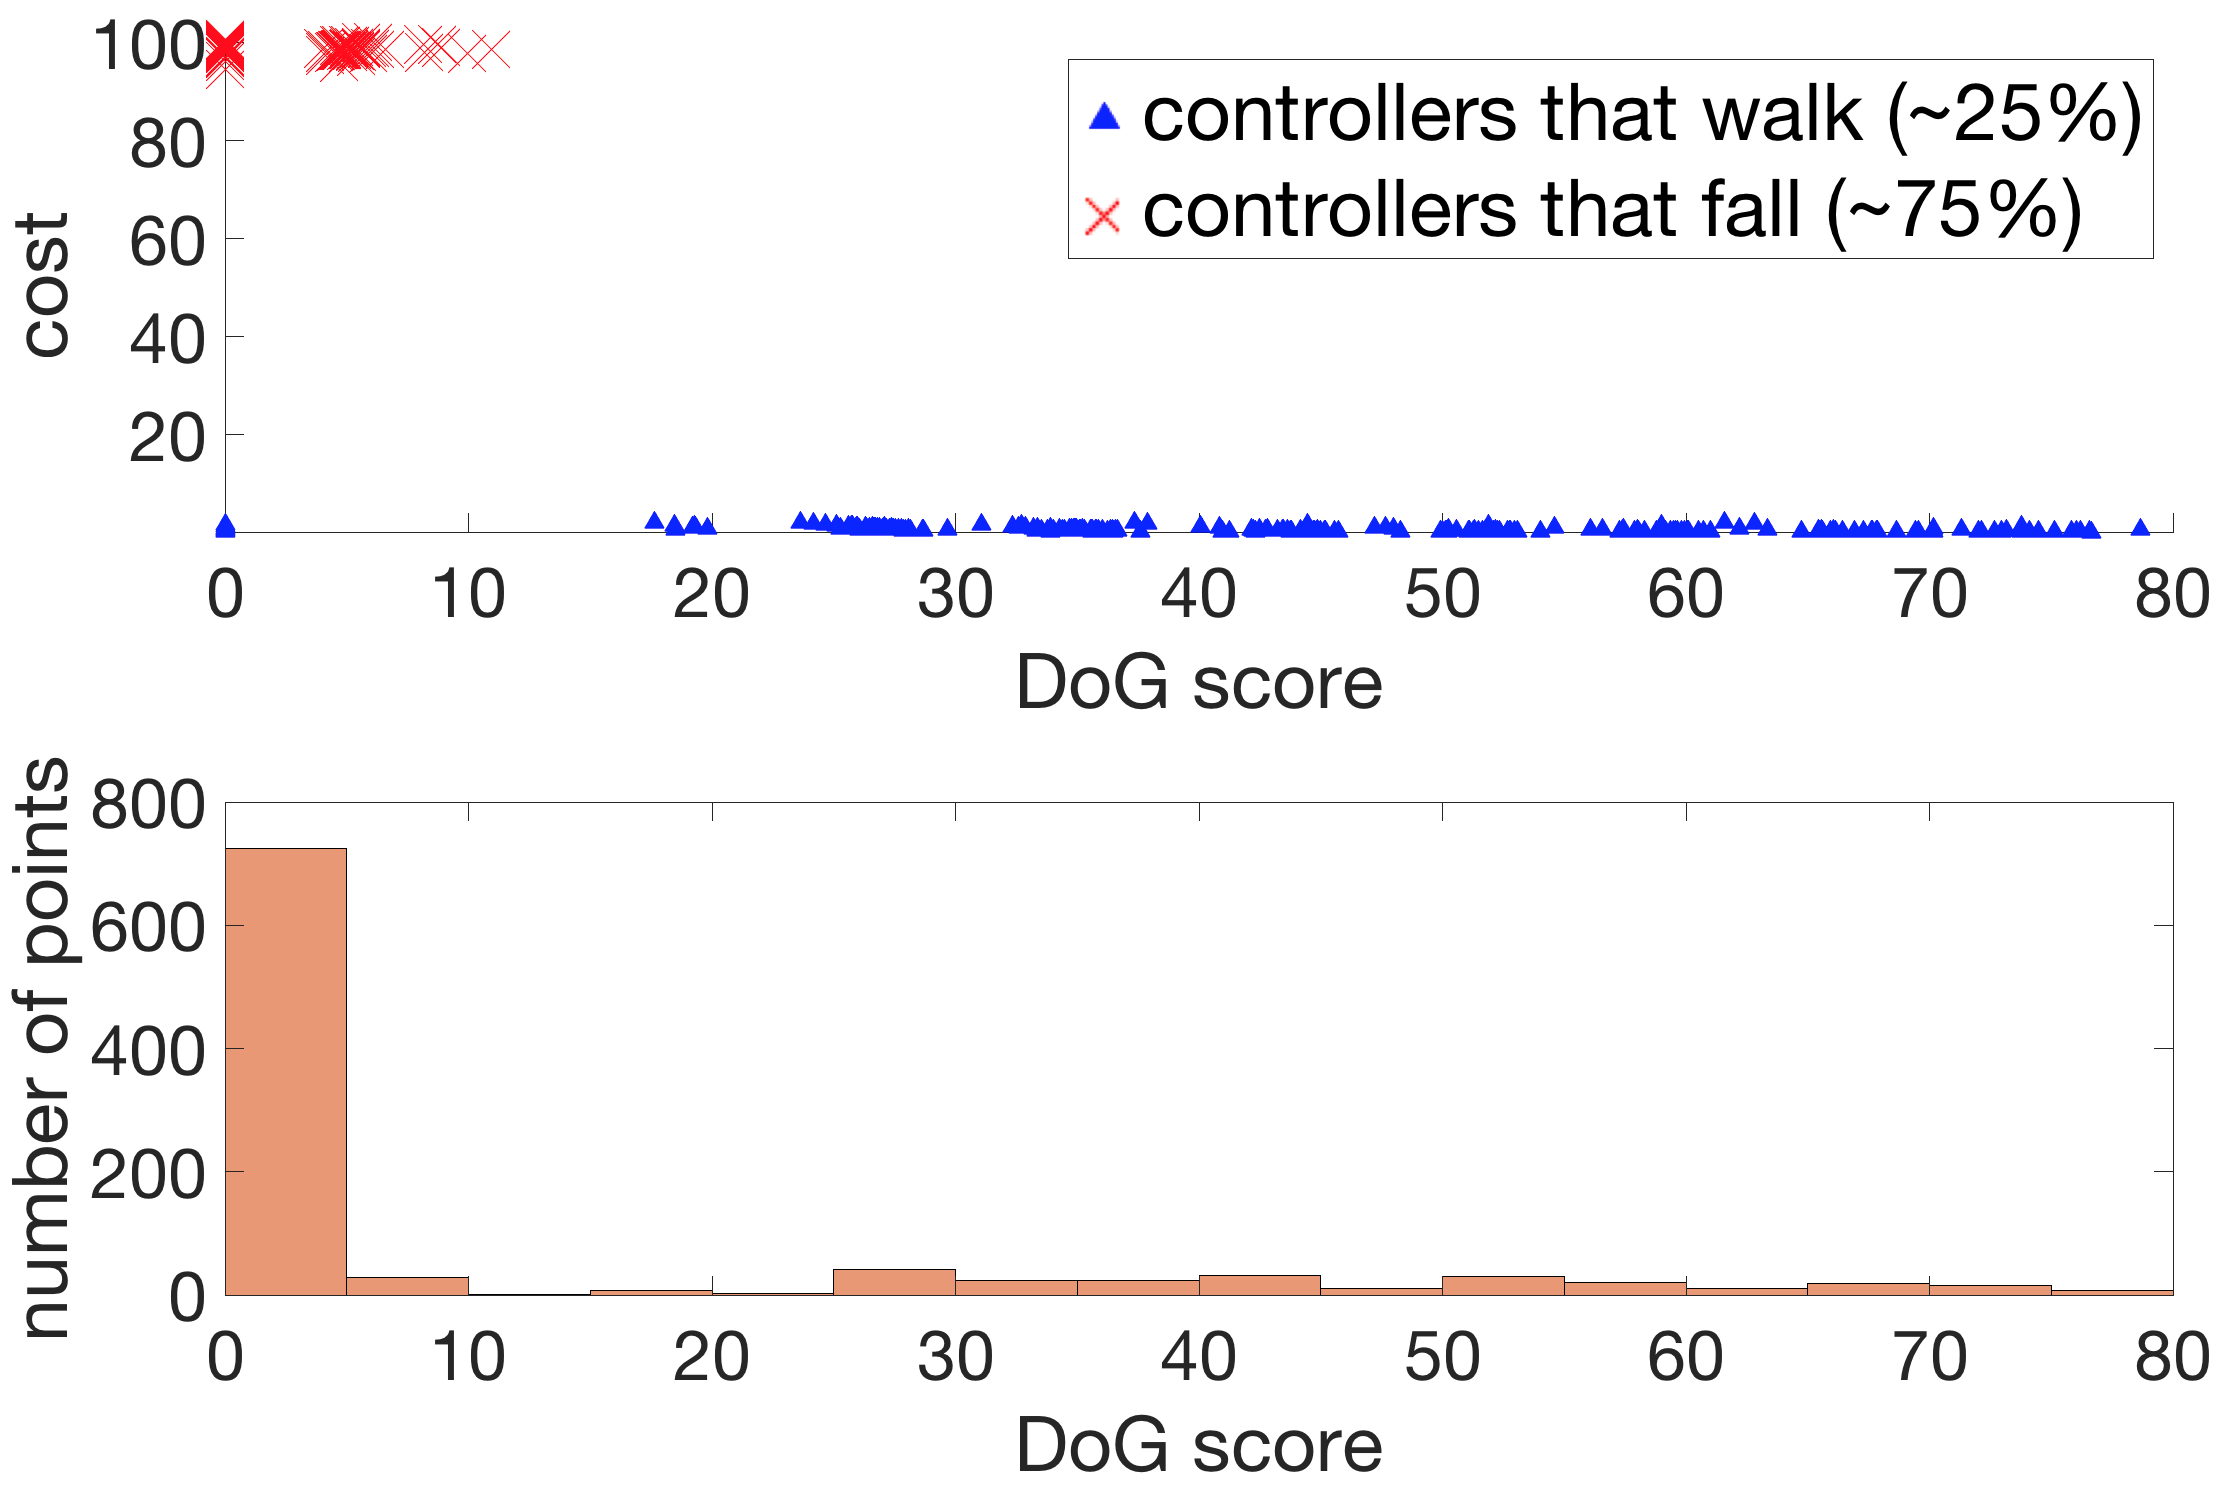
\includegraphics[width=0.75\textwidth]{img/dog_vs_cost_and_hist.png}
    \caption{\small{DoG score vs cost for 1000 randomly selected controller parameters (controller and cost from Sections~\ref{sec:raibert_cont},\ref{sec:exps_sim}). Lower DoG scores usually lead to higher costs and falling. A few points that step very fast (chatter)  don't fall in simulation, so can have low cost and low DoG score. But such points are very likely to fall on hardware.}}
            \vspace{-5mm}
    \label{fig:dogvsfit}
\end{figure}

The DoG score helps cluster controllers based on their behaviour in simulation. The hope is that behavioral cues like the ones described in metrics $M_{1-4}$ have a higher chance of transferring between simulation and hardware  than costs. On hardware, once we have evaluated a controller with a particular value of $\phi$, we expect controllers with similar values of $\phi$ to have a similar cost. This roughly splits the cost function landscape, separating points that can potentially walk, and those that cannot, as shown in Figure \ref{fig:dogvsfit}. Suppose we sample an unstable point with a low $\phi$ score and obtain a high cost on hardware (we can also seed our search with such points). We can then be fairly certain of other unstable points from simulation doing poorly as well. As a result, we can focus on potentially promising points to sample -- making the search more sample efficient and biased towards sampling safe points.


Note that in Equation \ref{eq:dog}, metrics $M_{1-4}$ are weighed equally when summing up. This over-condensed version is very efficient at finding walking controllers as it groups all non-walking controllers as one and separates them from all walking controllers. However, it is not good for distinguishing between walking controllers. In other words, if we are only searching for reasonably good walking controllers, and do not care about optimizing the quality of walking of each controllers, the 1 dimensional kernel is ideal for quickly reaching such a controller. However, if we care about the quality of walking, for example, we would like to walk at a particular speed, or minimize metabolic energy, the 1 dimensional kernel isn't ideal for distinguishing between such controllers.
A small but useful addition could be to learn the weights for a 4-dimensional feature transform $[M_1, M_2, M_3, M_4]$ using Automatic Relevance Determination (ARD), described in \cite{GPsMLBook}, before summing up. This would enable us to weigh the 4 metrics depending on their importance for a particular task, controller or robot. Another addition would be to use a 4-dimensional kernel, which might be less sample-efficient, but more robust to mismatch between simulation and hardware, as well as help optimize particular cost functions better. 


\subsection{A feature transform from data}

While hand-designed feature transforms can be very data-efficient, as well as shed light on what the optimization is prioritizing, they are not ideal for situations where such information is not available. In this section, we automatically learn an informed transform for optimizing bipedal locomotion controllers without extensive domain-expertise. We start by running short simulations in a high-fidelity simulator for the locomotion controller of interest. 
We run simulations for a large grid of parameter sets and record the resulting costs and simulation trajectories. Costs obtained during short simulations serve as approximate indicators of the quality of the controller parameters for longer simulations, though they can diverge later. Our idea is to use the behaviors obtained from simulation to generate an informed distance metric for the Bayesian optimization kernel. 

\subsubsection{Regression with Implicitly Asymmetric Loss}
\label{sec:approach_asym}

We consider a cost function focused on matching the desired walking speed and heavily penalizing falls:
\begin{equation}
cost_{sim} = 		
    \begin{cases}
		100 - x_{fall} , \text{\small{if fall}} \\
		10 \cdot || v_{tgt} - \pmb{v}_{actual} ||^2, \text{\small{if walk}}\\
	\end{cases}
\label{eq:cost_atrias}
\end{equation}
where $x_{fall}$ is the distance travelled before falling, $v_{tgt}$ is the target velocity and $\pmb{v}_{actual}$ is the vector containing actual velocities of the robot. This kind of cost function is of interest because it helps easily distinguish points that walk from points that fall. Similar costs have been considered in prior work when optimizing locomotion controllers~\citep{song2015neural}.

\begin{figure}[t]
\centering
\caption{\small{2D slice of the cost landscape.}}
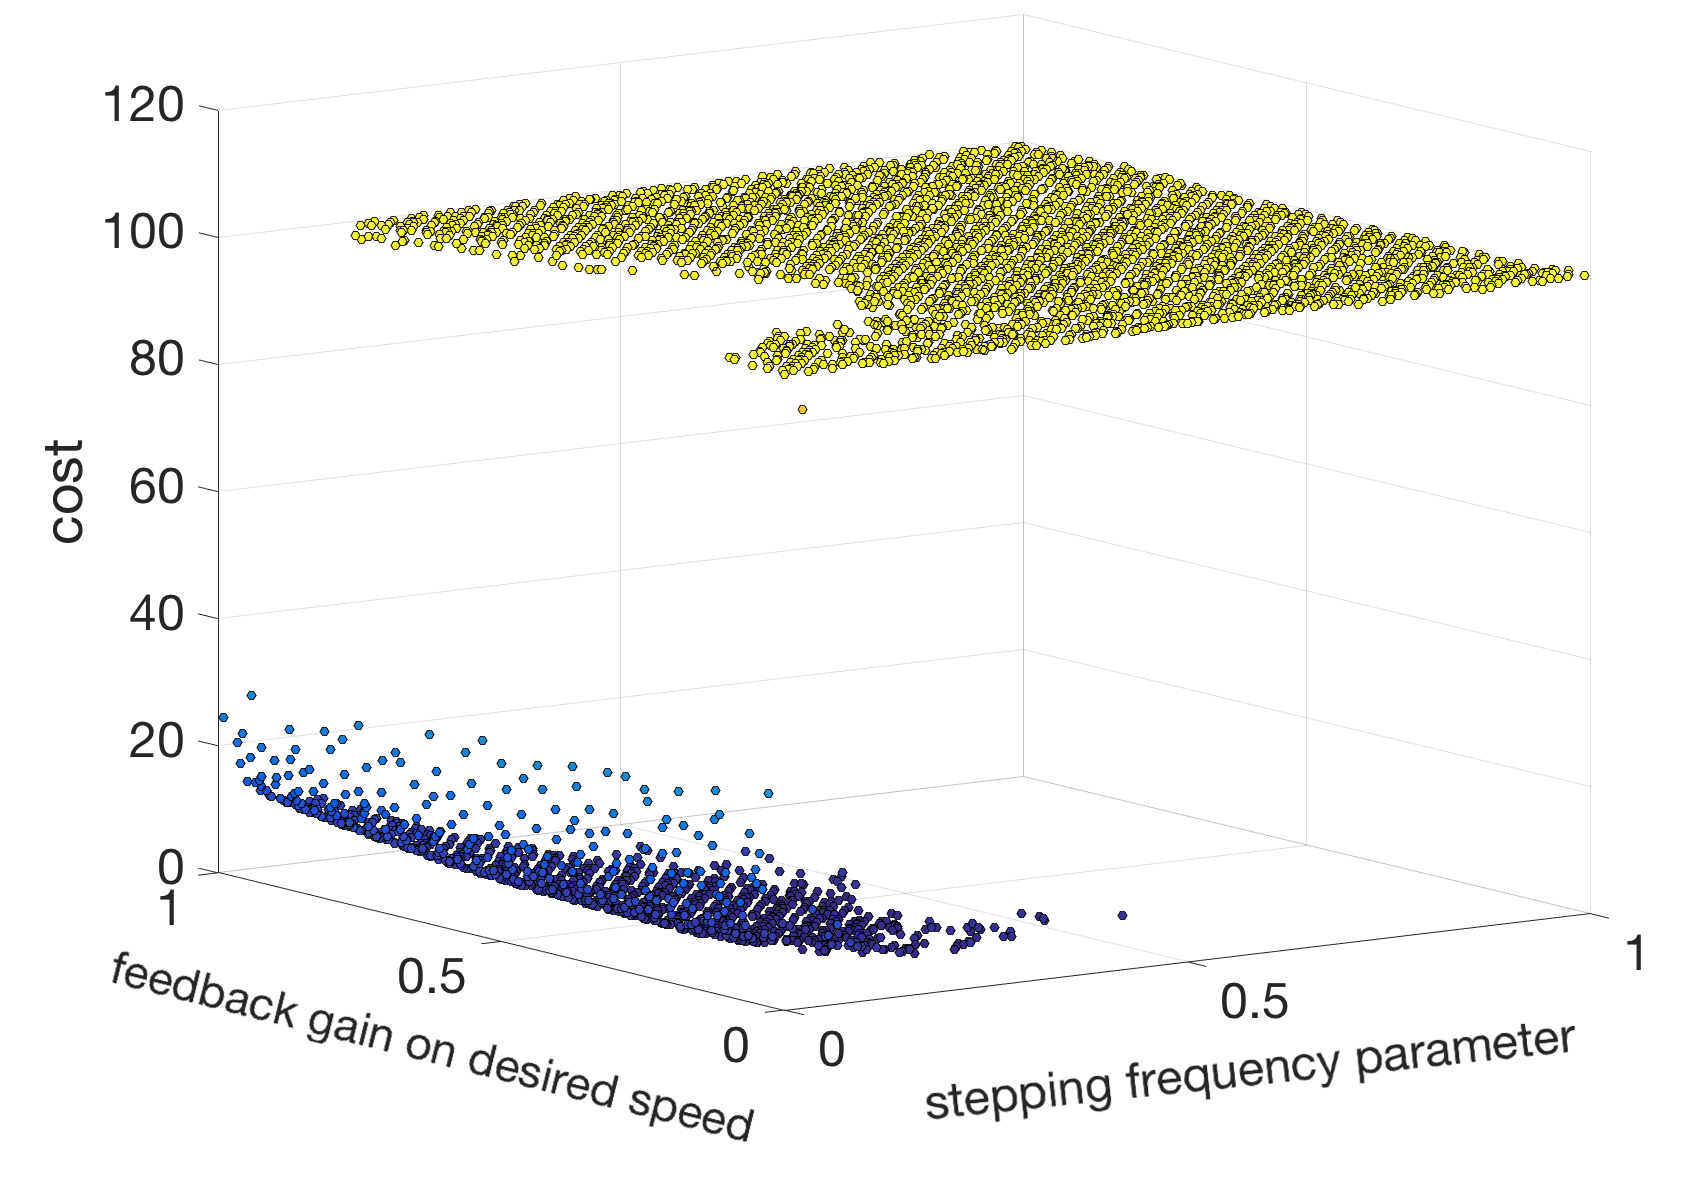
\includegraphics[width=0.7\textwidth]{img/costs_atrias.png}
\label{fig:atrias_cost_landscape}
\end{figure}

Figure~\ref{fig:atrias_cost_landscape} shows a scatter plot of applying cost from Equation~\ref{eq:cost_atrias} to simulations of a 5-dimensional controller for the ATRIAS robot as introduced in Section~\ref{sec:raibert_cont}. For visualization we only vary the 2 most sensitive dimensions, leading to a 2-dimensional subspace of the parameter space. We pick a well-performing set of parameters (in 5D), then vary the first two dimensions - the stepping frequency of the controller and the feedback gain on the desired speed. As seen in the figure, less than a quarter of this subspace contains points corresponding to low-cost simulation results (blue points on the scatter plot). 

The challenge comes from the fact that the boundary between the well-performing (blue) and poorly performing (yellow) parameters is discontinuous. This is a typical landscape for bipedal systems, where a controller that makes the robot fall is much worse than one than walks, and the boundary is extremely sharp. While there can be variations to how costs are structured among stable walking points -- efficiency vs speed vs distance covered, parameters that fall are much worse than those who don't. Fitting such cost function with regression can be difficult. Learning to reconstruct the boundary exactly using the training set might result in overfitting and poor performance on the test set. Trying to fix this by applying regularization is likely to result in high loss and uncertainty about the points close to the boundary. This is particularly problematic if poorly performing points lie close to some of the most promising regions of the parameter space, which is the case for the setting we consider. 
%\begin{figure}[t]
%\centering
%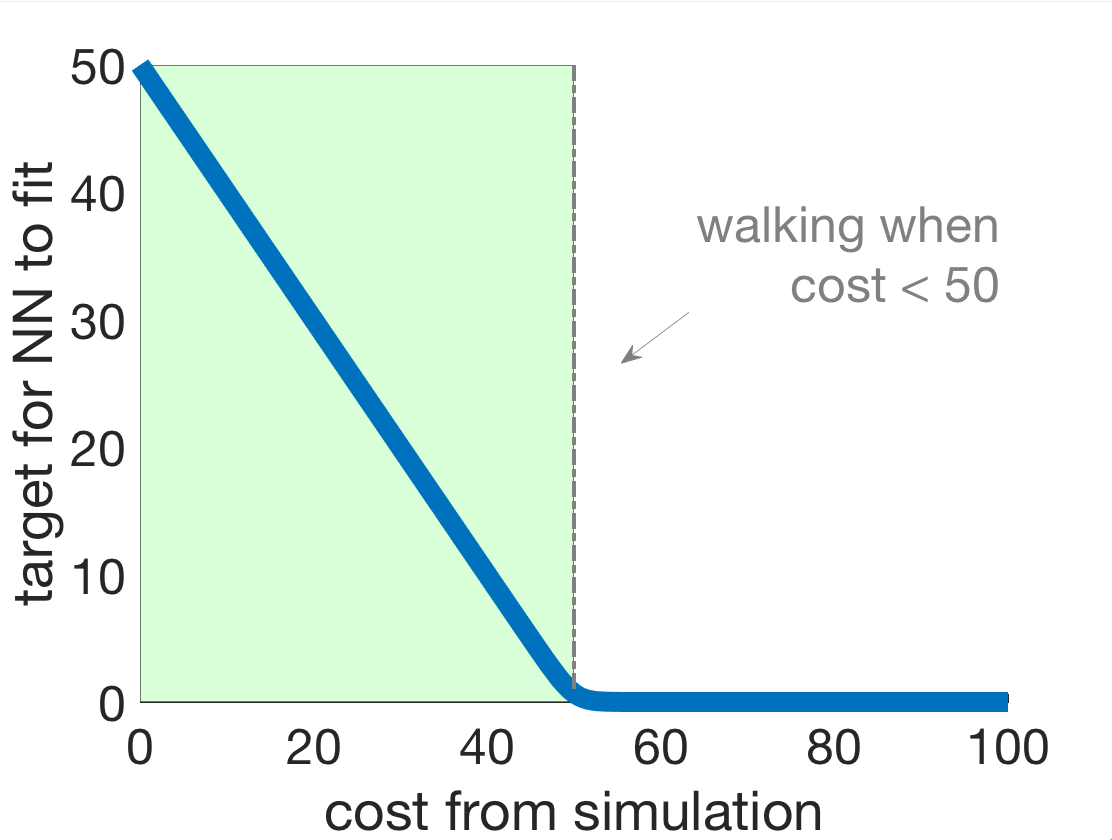
\includegraphics[width=0.35\textwidth]{img/softplus.png}
%\caption{\small{Softplus Cost transformation.}}
%\label{fig:atrias_cost_transform}
%\end{figure}
%Instead of a straightforward approach of learning to reconstruct the cost function directly, 
We propose to use a transformation of the cost as the target for the supervised learning. Our approach is to train a deep neural network to reconstruct a reflected shifted softplus function of the cost: 
\begin{equation}
\textit{score}_{\textit{NN}} = \zeta \big( cost_{walk} - cost_{sim}(\pmb{x}) \big)
\label{eq:score_asymnn}
\end{equation}
Here $\zeta$ is a softplus function: $\zeta(a) = ln\big( 1 + e^a \big)$, $cost_{walk}$ is the average cost for the parameter sets that walk during short simulations, $cost_{sim}(\pmb{x})$ is the cost computed by the simulator for vector $\pmb{x}$ of controller parameter values (Eq. \ref{eq:cost_atrias}). Using this transformation yields a ``score" function such that parameter sets which produce poor results in simulation are mapped to values close to zero. With this, the differences in scores of the poorly performing parameter sets become small or zero. In contrast, the differences in scores of the parameter sets yielding potentially promising results remain proportional to the difference in the corresponding costs. %Figure~\ref{fig:atrias_cost_transform} gives a visualization of this transformation.

Cost transformation in Equation~\ref{eq:score_asymnn} serves to essentially create an asymmetric loss for neural network training. This asymmetric loss is minimized when the promising (low-cost, high-score) points are reconstructed correctly.
%yielding linear relationship between the transformed scores and the original costs. 
For the poorly performing (high-cost, low-score) points, it only matters that the output of the neural network is close to zero. Such asymmetric loss can be interpreted as implementing a hybrid of regression and ``soft'' classification. The regression aspect aims to fit the promising points which correspond to parameters yielding walking behaviors. The ``soft'' classification causes an increase in the loss only if a poorly performing point is ``mis-classified'' as well-performing (output of the neural network is not close to zero). As a result, while the network still tries to perfectly fit the well performing points, it only needs to classify poorly performing points as poor.

The asymmetry in the loss is essential for training to reconstruct noisy costs with sharp discontinuities. Such cost functions are frequently used in optimization of locomotion controllers, with the aim to sharply penalize falling. This challenge is further addressed by learning to reconstruct the transformation of the cost (as discussed above) in combination with using a L1 loss, instead of the usual L2 loss when training the neural network. With this, errors in reconstructing points on the boundary contribute only linearly to the overall loss. This helps achieve a better fit of the stable parts of the parameter space, instead of focusing on the boundary.
%avoid focusing too much on fitting the hard-to-reconstruct uncertain region in favor of learning a better fit of other more stable parts of the parameter space.

The resultant transform $\phi(\pmb{x})$ from this cost based transform is the output of the neural network:
\begin{equation}
    \phi(\pmb{x}) = score_{NN}(\pmb{x})
\end{equation}


We utilize the reconstructed transformed costs to define $\textit{asymNN}$ kernel for Bayesian Optimization:
\begin{align}
    k(\pmb{x}_i, \pmb{x}_j) \rightarrow k(\phi(\pmb{x}_i), \phi(\pmb{x}_j)) \\
    k_{asymNN}(\pmb{x}_i, \pmb{x}_j) = \sigma_k^2 \exp\Big(- \frac{1}{2 \pmb{l}^2} \|\phi(\pmb{x}_i) - \phi(\pmb{x}_j)\|^2 \Big),
\end{align}
with hyperparameters $\sigma_k, \pmb{l}$.
The proposed approach is able to clearly separate the unpromising part of the parameter space. Under the resulting distance metric poorly performing sets of parameters are close together and far from well-performing ones. 
A smaller priority is given to high-precision reconstruction of the poorly performing region of the parameter space. This is desirable, since it has been observed that usually simulators are optimistic compared to the real word~\citep{cutler2015real}. This is indeed the case with the locomotion simulators we consider: if a set of controller parameters causes falling or instability in simulation, it is very unlikely that the same controller parameters would result in successful walking when applied to real hardware. With that, distinguishing all the various ways in which poorly performing points fail is not useful. Using \textit{asymNN} kernel helps rapidly separate bad regions of the parameter space from the regions that might contain promising points. 

\subsubsection{Reconstructing Cost-agnostic Trajectory Summaries}
\label{sec:approach_traj}

While learning a distance metric from the cost could be effective for a wide variety of problems, frequently there is a need for a cost-agnostic approach. Such cases arise when the data from the simulator is computationally expensive to collect and we need to change the cost function. Different tasks might call for slightly different cost functions. For example, high energy consumption could be penalized if energy use needs to be restricted; robustness of the walk could be emphasized if only stable walking is acceptable; if achieving the desired speed is the most important factor -- then the cost might instead only reflect how well the desired speed is maintained. For such cases we propose to train a neural network to reconstruct summaries of trajectories that are cost-agnostic, then utilize these trajectory summaries for constructing kernel distance metric.

In most cases, a summary of trajectory information contains all the pertinent information. Hence, we focus on collecting the following aspects of the simulated trajectories: walking time (time before falling), energy used during walking, position of the torso, angle of the torso, coordinates of the center of mass at the end of the short simulation runs. These summaries of simulated trajectories are collected for a range of controller parameters and comprise the training set for the neural network to fit (input: $\pmb{x}$ -- a set of control parameters; output: $\pmb{traj_x}$ -- the corresponding trajectory summary obtained from simulation). The outputs of the (trained) neural network offer the reconstructed/approximate trajectory summaries:
\begin{equation}
    score_{\textit{trajNN}}(\pmb{x}) = \pmb{\widehat{traj}_x}
\end{equation}
where $\pmb{x}$ is the input controller parameters, and $\pmb{\widehat{traj}_x}$ is the corresponding reconstructed trajectory summary.
These are then used to define a distance metric for the kernel for Bayesian Optimization:
\begin{align}
\phi(\pmb{x}) = score_{trajNN}(\pmb{x})\\
k_{\textit{trajNN}}(\pmb{x}_i, \pmb{x}_j) = \sigma_k^2 \exp\Big(- \frac{1}{2 \pmb{l}^2} \|\phi(\pmb{x}_i) - \phi(\pmb{x}_j)\|^2 \Big)
\end{align}
with hyperparameters $\sigma_k, \pmb{l}$ .

The general concept of utilizing trajectory data to improve sample efficiency of BO has been proposed before, for example in~\cite{wilson2014using}. However, prior work assumed obtaining trajectory data is possible every time kernel values $k(\pmb{x}_i, \pmb{x}_j)$ need to be evaluated. This is not the case in our setting, as each controller has to be evaluated to obtain the simulation trajectory. To overcome this, we obtain trajectory summaries via costly high-fidelity simulations. To avoid having to run simulations while performing BO on hardware, we train a neural network to learn reconstructing trajectory summaries first. Running a forward pass of the neural network is a relatively inexpensive operation, hence reconstructed/approximate trajectory summaries can be quickly obtained during BO whenever $k_{\textit{trajNN}}(\pmb{x}_i, \pmb{x}_j)$ needs to be computed. Note that the trajectory information we extract is generic and can be applied to other problems without requiring in-depth domain knowledge. When applying this approach to a new domain, the strategy would be to include trajectory information used to compute cost functions that are of interest/relevance in the domain. For example, for a manipulator, the coordinates of  end-effector(s) could be recorded at relevant points. In contrast, information extracted in \cite{rai2016sample, cully2015robots} are more domain specific.

In addition to offering a cost-agnostic approach, our trajectory-based kernel retains more information about important aspects of simulated trajectories than a cost-based  kernel. We observe that this re-parameterization could be more effective than a cost-based kernel in cases when the kernel does not retain enough information to effectively optimize the acquisition function used in Bayesian Optimization, due to over-condensing the characteristics of the simulation. In particular, cost-based kernel offers most sample-efficient results in the case of using lower-dimensional controller and the case of using a smooth cost with a higher-dimensional controller - basically easier to optimize problems. On more challenging discontinuous costs and high-dimensional controllers, trajectory-based kernel outperforms cost-based kernel.
The trajectory-based kernel also significantly outperforms standard Bayesian Optimization, even when the optimization uses challenging discontinuous costs. 
%In the experiments section we compare the performance of the kernel based on 8-dimensional trajectory summaries with that of a 1-dimensional cost-based kernel. 

%\AR{Add the pipeline picture at the top of this page.}

\section{Modelling mismatch between simulation and hardware}
\label{sec:mismatch}
While all the generalized transform $\phi$ proposed in the previous section can successfully characterize the quality of a gait, large mismatch between a simulator and real-world hardware could still present a challenge. Some controller parameters could yield good gait characteristics in a short simulation, but perform poorly during a longer trial on hardware or simulation. While this issue did not arise during our hardware experiments with the controller described in Section~\ref{sec:raibert_cont}, this could be an issue with a different and higher-dimensional controller and inaccurate simulator. Hence, it is important to study how the performance worsens as the fidelity of the simulator decreases and how the kernel can be adjusted to compensate for this mismatch.

In ~\cite{rai2017bayesian}, we proposed a way to incorporate information about simulation-hardware mismatch into the kernel from the samples evaluated so far. We augment the simulation-based kernel to include this additional information about mismatch, by expanding the original kernel by an extra dimension that contains the predicted mismatch for each controller $\pmb{x}$.
 
A separate Gaussian process is used to model the mismatch experienced on hardware, starting from an initial prior mismatch of 0: $g(\pmb{x})\!\sim\!\mathcal{GP}(0, k_{SE}(\pmb{x}_i,\pmb{x}_j))$.
For any evaluated controller $\pmb{x}_i$, we can compute the difference between $\phi(\pmb{x}_i)$ in simulation and on hardware: 
\begin{equation}
    d_{\pmb{x}_i}\!=\!\phi^{sim}(\pmb{x}_i) \!-\! \phi^{hw}(\pmb{x}_i)    
\end{equation}
 
We can now use mismatch data $\{ d_{\pmb{x}_i} | i=1...n \}$ to construct a model for the expected mismatch: $\bar{g}(\pmb{x})$. In the case of using a GP-based model, $\bar{g}(\cdot)$ would denote the posterior estimate of expected mismatch. With this, we can predict simulation-hardware mismatch in the original space of controller parameters for unevaluated controllers. Combining this with kernel $k_{\phi}$ we obtain an adjusted kernel:
\begin{align}
\label{eq:k_adj}
\begin{split}
    \pmb{\phi}^{adj}_{\pmb{x}} = \begin{bmatrix} \phi^{sim}(\pmb{x}) \\ \bar{g}(\pmb{x}) \end{bmatrix}, \quad \quad \quad \quad \quad \quad 
    \pmb{t}_{ij}^{adj} \!=\! \pmb{\phi}^{adj}_{\pmb{x}_i} \!-\! \pmb{\phi}^{adj}_{\pmb{x}_j} \\
    k_{\phi_{adj}}(\pmb{x}_i, \pmb{x}_j) = \sigma_k^2 \exp\Big(- \tfrac{1}{2} (\pmb{t}_{ij}^{adj})^T \diag\Big(\begin{bmatrix}\pmb{\ell_1} \\ \pmb{\ell_2} \end{bmatrix}\Big)^{\!-\!2} \pmb{t}_{ij}^{adj} \Big) \\
\end{split}
\end{align}

The similarity between points $\pmb{x}_i, \pmb{x}_j$ is now dictated by two components: representation in $\phi$ space and expected mismatch. This construction has an intuitive explanation: Suppose controller $\pmb{x_i}$ results in walking when simulated, but falls during hardware evaluation. $k_{\phi_{adj}}$ would register a high mismatch for $\pmb{x}_i$. Controllers would be deemed similar to $\pmb{x}_i$ only if they have both similar simulation-based $\phi(\cdot)$ and similar estimated mismatch $\bar{g}(\cdot)$. Points with similar simulation-based $\phi(\cdot)$ and low predicted mismatch would still be `far away' from the failed $\pmb{x}_i$. This would help BO sample points that still have high chances of walking in simulation, but are in a different region of the original parameter space that $\pmb{x}_i$. In the next section, we present a more mathematically rigorous interpretation for $k_{\phi_{adj}}$.




%With this construction, if there is a mismatch in simulation vs hardware, the problematic region will have a high adjusted DoG kernel distance to regions without the mismatch.
We will call this adjusted kernel with hardware and simulation mismatch the adjusted \dogkernel in the future.
This formulation is similar in spirit to other approaches, such as \cite{marco2017virtual}. However, while previous work ``mistrusts" all simulation data, our formulation lets us fit a dynamic mismatch function from data. This lets us trust the simulation in some regions, while mistrust it in others.

There are several approaches in literature that attempt to model the difference between simulation and hardware. \cite{wilson2014using} propose modelling the mismatch between a learned model and the real system by a second ``residual" GP. They predict the expected cost at a new point using a convex combination of two GPs:  
\begin{align}
    J(\pmb{x}) = (1-\beta) J_{sim}(\pmb{x}) + \beta J_{err}(\pmb{x}) \\
    J_{err}(\pmb{x}) \sim \mathcal{GP}(0, k(\pmb{x},\pmb{x}')) \\ 
    J_{sim}(\pmb{x}) \sim \mathcal{GP}(m_{sim}(\pmb{x},\pmb{x}_i,...,\pmb{x}_n), k(\pmb{x},\pmb{x}'))
\end{align}
$\beta$ can be learned from data. $J_{err}$ models the residual between the simulation model and the actual data, initialized with a 0 prior. $J_{sim}$ is a cost model learned over simulation points $m_{sim}(\pmb{x},\pmb{x}_i,...,\pmb{x}_n)$, which are be an inaccurate representation of the actual system. The resultant GP has a mean which is a convex combination of the two GP means, and the same variance as the chosen $k$. While this approach can be very powerful when the simulation is close to hardware, with significant mismatch the bias of simulation can be hard to overcome.

In contrast, our approach puts majority of the information from simulation into the kernel, which is an easier to overcome biased prior information. We present a more mathematical foundation for our mismatch model in the next section. Results comparing our approach to other approaches from literature are in Section \ref{sec:}


Multiple sources of information can also be added to Gaussian Processes \citep{poloczek2016multi}. For example, let the true cost be a combination of cost in simulation and a residual error - each with a separate kernel:
\begin{equation}
    J(\pmb{x}) = J_{sim}(\pmb{x}) + J_{err}(\pmb{x})
\end{equation}
where
\begin{align}
     J_{err}(\pmb{x}) &\sim \mathcal{GP}(0, k_{err}(\pmb{x},\pmb{x}')) \\
J_{sim}(\pmb{x}) &\sim \mathcal{GP}(\mu_{sim}(\pmb{x}), k_{sim}(\pmb{x},\pmb{x}'))
\end{align}

Here $J(\pmb{x})$ is the true cost of the controller on hardware, $J_{sim}(\pmb{x})$ is a measurement from simulation, and $J_{err}(\pmb{x})$ is the noise distribution, which is the mismatch between simulation and hardware. Points sampled from hardware do not have this mismatch, and hence are samples from the true GP $J(\pmb{x})$. However points from simulation are samples from $J_{sim}(\pmb{x})$ and their corresponding residual $J_{err}$ needs to be estimated. 

\cite{poloczek2016multi} extend the kernel by an additional binary
variable $\delta$, which indicates whether the cost is evaluated in
simulation $(\delta = 0)$ or on the physical system $(\delta = 1)$. Based on the extended parameter $a = (\pmb{x}, \delta)$, we can model the cost
by adapting the kernel of $J$ to
\begin{equation}
    k(\pmb{x}, \pmb{x'}) = k_{sim}(\pmb{x}, \pmb{x'}) + \delta \delta' k_{err}(\pmb{x}, \pmb{x'})
\end{equation}
\cite{marco2017virtual} develop an automatic way of trading off data from simulation and hardware based on the expected improvement of each source, normalized by the time cost of sampling simulation vs hardware. 
%\pagebreak

 %Figure \ref{fig:bo_sim_hdw} shows a toy-example of using the approach from \cite{poloczek2016multi} in Bayesian Optimization. 10 points are sampled from simulation with uniform uncertainty everywhere (top). 2 points are added from hardware with low uncertainty (bottom). Since there is still uncertainty in the potentially low performing regions, BO wastes a sample on unpromising region. 
 
 
 %Figure \ref{fig:bo_sim_hdw_var} shows an example with non-uniform noise in the simulation space. We can be fairly certain of the potentially poorly performing points, even if the exact value of the cost might be different. This makes the BO not sample any unpromising points in the unpromising region on hardware. Hence it samples very close to optimum in as few as 2 samples. This toy-example motivates the need for variable uncertainty over the controller space to enhance sample-efficiency. 
 
 
 %If we modelled the mismatch from data, and incorporated it into the kernel in a similar manner, our resultant adjusted \dogkernel would become : 
%\begin{equation}
%    k_{adj}(\pmb{x_i}, \pmb{x_j}) = \sigma^2_k \exp\Big( -\frac{1}{2l_k^2} \big( \phi_(\pmb{x_i}) - \phi_(\pmb{x_j}) \big)^2 \Big) +  \sigma^2_m \exp \Big( -\frac{1}{2l_m^2} \big( g_*(\pmb{x_i}) - g_*(\pmb{x_j}) \big)^2 \Big) 
%\end{equation}

%Instead of adding the mismatch to the feature transform $\phi$, resulting in a product kernel as in Equation \ref{eq:kernel_prod}, we could add the distance between the mismatch at two points to their kernel distances. We would like to experiment with the various ways of modelling mismatch in literature and apply it to our problem.

%While existing methods in literature talk about variable mismatch maps for different regions of state space, to the best of our knowledge, there isn't any experiments on a real system. 
For high dimensional controllers, these error maps can  need a lot of data to accurately model the inaccuracy of simulation, especially for rapidly changing discontinuous costs. To overcome this problem, it is worth exploring if characteristics of simulation can be used to create a prior mismatch. For example, controllers with higher impacts might have a high chance of falling on hardware even if they walk in simulation. Similarly, controllers that venture close to joint limits might be likely to fail on hardware, even if successful in simulation. 

In comparison, building a mismatch map for the reduced dimensional DoG-space can be very data efficient. This allows us to compensate for the mismatch between simulation and hardware and propogate this information back to update the features collected in simulation. This leads to a novel way of updating models from hardware data in a transformed space with very few data points. Moreover, if the simulation is close to hardware in some regions, the learned mismatch is close to 0 and higher in other regions where the simulation is different from the hardware.

\subsection{Interpretation of Kernel with Mismatch Modeling}

In this section we give a more mathematically sound interpretation the mismatch adjusted kernel described in the previous section.

Let us consider a controller $\pmb{x}_i$ evaluated on hardware. The difference between simulation-based and hardware-based feature transform for $\pmb{x}_i$ is $d_{\pmb{x}_i} = \phi^{sim}(\pmb{x}_i) - \phi^{hw}(\pmb{x}_i)$. The `true' hardware feature transform for $\pmb{x_i}$ is $\phi^{hw}(\pmb{x_i}) = \phi^{sim}(\pmb{x_i}) - d_{\pmb{x_i}}$. After $n$ evaluations on hardware, $\{ d_{\pmb{x}_i} | i=1...n \}$ can serve as data for modeling simulation-hardware mismatch. In principle, any data-efficient model $g(\cdot)$ can be used, such as GP (a multi-output GP in case $\phi(\cdot)$ $>1D$). With this, we can obtain an adjusted transform: $\hat{\phi}^{hw}(\pmb{x}) = \phi^{sim}(\pmb{x}) - \bar{g}(\pmb{x})$, where $\bar{g}(\cdot)$ is the output of the model fitted using $\{d_{\pmb{x}_i} | i=1,...n \}$.

Suppose $\pmb{x}_{new}$ has not been evaluated on hardware. We can use $\hat{\phi}^{hw}(\pmb{x}_{new}) = \phi^{sim}(\pmb{x}_{new}) - \bar{g}(\pmb{x}_{new})$ as the adjusted estimate of what the output of $\phi$ should be, taking into account what we have learned so far about simulation-hardware mismatch.

Let's construct kernel $k^{v_2}_{\phi_{adj}}(\pmb{x}_i, \pmb{x}_j)$ that uses these hardware-adjusted estimates directly:
\begin{equation*}
\begin{split}
\pmb{q}_{ij}^{adj} &= \hat{\phi}^{hw}(\pmb{x}_{i}) - \hat{\phi}^{hw}(\pmb{x}_{j}) \\
&= (\phi^{sim}(\pmb{x}_{i}) - \bar{g}(\pmb{x}_i)) - (\phi^{sim}(\pmb{x}_{j}) - \bar{g}(\pmb{x}_j) ) \\
&= \underbrace{(\phi^{sim}(\pmb{x}_{i}) - \phi^{sim}(\pmb{x}_{j}))}_{\pmb{v}_{\phi}} + \underbrace{(\bar{g}(\pmb{x}_j) - \bar{g}(\pmb{x}_i) )}_{\pmb{v}_{g}}
\end{split}
\end{equation*}

\begin{equation*}
\begin{split}
k^{v_2}_{\phi_{adj}}(\pmb{x}_i, \pmb{x}_j) &= \sigma^2_{k_{v_0}} \exp\Big(- \tfrac{1}{2} (\pmb{q}_{ij}^{adj})^T \diag(\pmb{\ell})^{\!-\!2} \pmb{q}_{ij}^{adj} \Big) \\
& = \sigma^2 \exp\Big(- \tfrac{1}{2} \big[ (\pmb{v}_{\phi} + \pmb{v}_{g})^T \diag(\pmb{\ell})^{\!-\!2} (\pmb{v}_{\phi} + \pmb{v}_{g}) \big] \Big) \\
& = \sigma^2
\exp\Big(- \tfrac{1}{2} \big[ \pmb{v}_{\phi}^T \diag(\pmb{\ell})^{\!-\!2} \pmb{v}_{\phi} + \pmb{v}_{g}^T\diag(\pmb{\ell})^{\!-\!2} \pmb{v}_{g} + prod_{ij} \big] \Big)\\
&\quad \quad \quad \quad \quad \text{where } prod_{ij} = 2 \pmb{v}_{\phi}^T\diag(\pmb{\ell})^{\!-\!2} \pmb{v}_{g}
\end{split}
\end{equation*}

Using $\exp(a+b+c)=\exp(c) \cdot \exp(a+b)$,  we have:
\begin{align*}
k^{v_2}_{\phi_{adj}}(\pmb{x}_i, \pmb{x}_j) &= \sigma^2 \exp(-prod_{ij}) \exp\Big(- \tfrac{1}{2} \big[ \pmb{v}_{\phi}^T \diag(\pmb{\ell})^{\!-\!2} \pmb{v}_{\phi} + \pmb{v}_{g}^T\diag(\pmb{\ell})^{\!-\!2} \pmb{v}_{g} \big] \Big)
\end{align*}

If we now observe that $\pmb{v}_{g}^T\diag(\pmb{\ell})^{\!-\!2} \pmb{v}_{g} = (-\pmb{v}_{g})^T\diag(\pmb{\ell})^{\!-\!2} (-\pmb{v}_{g})$ we get:
\begin{align*}
k^{v_2}_{\phi_{adj}}(\pmb{x}_i, \pmb{x}_j) 
&= \sigma^2 \exp(-prod_{ij}) \exp\Big(- \tfrac{1}{2} (\pmb{t}_{ij}^{adj})^T \diag\Big(\begin{bmatrix}\pmb{\ell} \\ \pmb{\ell} \end{bmatrix} \Big)^{\!-\!2} \pmb{t}_{ij}^{adj} \Big) \\
\pmb{t}_{ij}^{adj} &= 
\begin{bmatrix}
\phi^{sim}(\pmb{x}_{i}) - \phi^{sim}(\pmb{x}_{j}) \\
\bar{g}(\pmb{x}_i) - \bar{g}(\pmb{x}_j)
\end{bmatrix} \text{ (from Equation~\ref{eq:k_adj})}
\end{align*}

Compare this to $k_{\phi_{adj}}$ from Equation~\ref{eq:k_adj}:
\begin{equation}
k_{\phi_{adj}}(\pmb{x}_i, \pmb{x}_j) = \sigma_k^2 \exp\Big(- \tfrac{1}{2} (\pmb{t}_{ij}^{adj})^T \diag\Big(\begin{bmatrix}\pmb{\ell_1} \\ \pmb{\ell_2} \end{bmatrix}\Big)^{\!-\!2} \pmb{t}_{ij}^{adj} \Big)
\end{equation}
Now we see that $k^{v_2}_{\phi_{adj}}$ and $k_{\phi_{adj}}$ have a similar form. Hyperparameters $\pmb{\ell_1}, \pmb{\ell_2}$ provide flexibility in $k_{\phi_{adj}}$ as compared to having only vector $\pmb{\ell}$ in $k^{v_2}_{\phi_{adj}}$. They can be adjusted manually or with Automatic Relevance Determination \citep{GPsMLBook}. 
For $k^{v_2}_{\phi_{adj}}$, the role of signal variance is captured by $\sigma^2 \exp(-prod_{ij})$. This makes the kernel nonstationary in the transformed $\phi$ space. 
Since $k_{\phi_{adj}}$ is already non-stationary in $\pmb{x}$, it is  unclear whether non-stationarity of $k^{v_2}_{\phi_{adj}}$ in the transformed $\phi$ space has any advantages.

The above discussion shows that $k_{\phi_{adj}}$ proposed in ~\cite{rai2017bayesian} is motivated both intuitively and mathematically. It aims to use a transform that accounts for the hardware mismatch, without adding extra non-stationarity in the transformed space. It also helps propagate data seen on hardware back to simulation, thus updating simulation models in a sample-efficient manner. If one has intuitions about the mismatch in the space of controllers, they could be used in the prior of the mismatch kernel to improve sample-efficiency further. 

\section{Transfer learning with contextual Bayesian optimization}


It is possible to transfer knowledge between tasks using Bayesian optimization by adding context to the learning. Contexts can include specific features of the experiment such as target speed of walking, or the incline of the ground. In such cases, the cost observed on hardware is a function of not just the controller parameters $\pmb{x}$, but also the context $c$, leading to a cost of the form $f(\pmb{x},c)$. Since the context is an observed variable, and not an optimized variable, Bayesian optimization is done on the parameters $\pmb{x}$, which conditioning the posterior of the GP on the observed $c$.

\begin{align}
    f(\pmb{x},c) \sim \mathcal{GP}(\mu(\pmb{x}, c), k((\pmb{x},c),(\pmb{x}',c'))) \\
    \pmb{x}_{t+1} = \argmax EI(f(x,c)|c=c_{observed})
\end{align}

Additionally, the feature transform in simulation can be a function of $c$, as well as the updates learned on hardware. The features observed on hardware $\phi^{w}(\pmb{x}, c)$ depend on both the controller as well as context. Hence the mismatch GP is also a function of both as $d_{\pmb{x}_i, c} = \phi^{sim}(\pmb{x_i},c)- \phi^{hw}(\pmb{x_i},c)$. Even if we do not know the contexts when calculating simulation features, the mismatch update gives us a way of building a context-dependant feature transform from data. Figure \ref{fig:context} shows an example where BO was conducted on 6 different target speeds for a 50-dimensional neuromuscular controller on the ATRIAS biped. 


The target speeds were $[0.5, 1.0, 1.5, 0.75, 1.25, 0.25, 1.75] m/s$. Initial speeds of $[0.5, 1.0, 1.5]m/s$ were simulated for 10 trials while latter speeds were simulated for 5. 
As shown in the figure, fewer trials are needed to reliably reach walking controllers as more data is added to the GP. This shows that learning on other target speeds indeed speeds up the learning for future targets, even when extrapolating. Target speeds of  $[0.75, 1.25, 0.25, 1.75] m/s$ reach a mean cost of $11.96$ after 5 trials, as compared to a mean cost of $19.61$ for the initial target speeds.

\begin{figure}
    \centering
    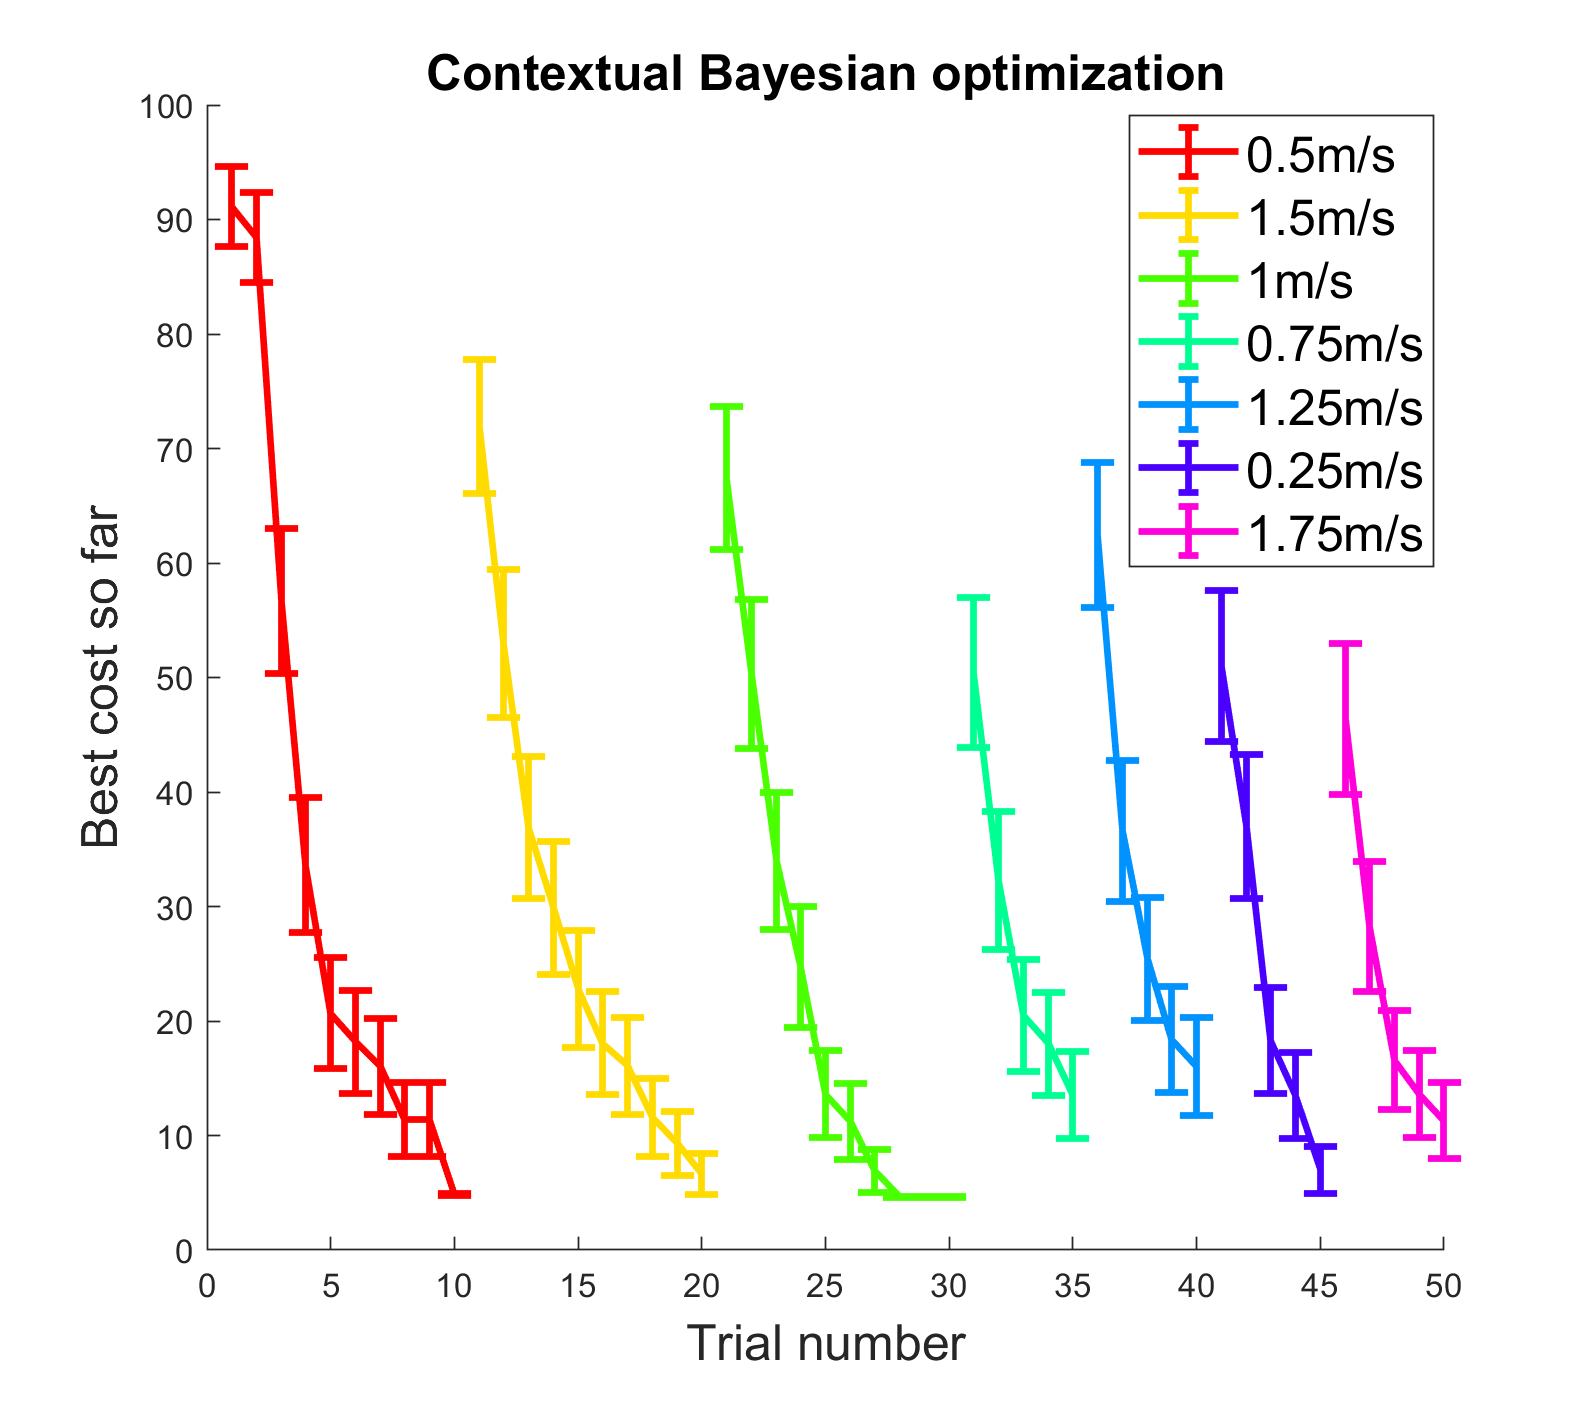
\includegraphics[width = 0.8\textwidth]{img/contexxt_bo.png}}
    \caption{Transfer learning with contextuan bayesian optimization can be used to transfer knowledge between different target speeds. Initial speeds of $[0.5, 1.0, 1.5]m/s$ were simulated for 10 trials while latter speeds of $[0.75, 1.25, 0.25, 1.75] m/s$ were simulated for 5 trials. The latter speeds reach a mean cost of $11.96$ after 5 trials, as compared to a mean cost of $19.61$ for the initial target speeds.}
    \label{fig:context}
\end{figure}
\chapter{Robots and controllers evaluated}
\label{chap:robots}
In this chapter, we describe the experimental setup conducted to validate our approach. Since this thesis is focused on using simulation to speed up hardware experiments, robot experiments form an important part of this work. Our hardware experiments are done on the ATRIAS robot on a boom. It is mounted on a pivot to planarize the robot to two dimensions, but it can still fall down. We present results on a feedback based reactively stepping controller, optimizing 5 and 9 parameters in 2 sets of experiments on hardware. 

Our simulation experiments are conducted on two different robot morphologies -- a planar 7-link biped model, and an ATRIAS simulation on the boom. We present two neuromuscular walking controllers -- on a 7-link biped optimizing 16 parameters, and then on an ATRIAS simulation optimizing 50 parameters. We also build inaccurate simulations of ATRIAS and test the effect of increasing mismatch between simulation and hardware on performance on Bayesian optimization.

In addition, we present experiments on learning neural network policies using deep reinforcement learning. These policies are learned in ATRIAS simulation and deployed on the ATRIAS biped.

We detail our robots in the next section, followed by the controllers. 

\section{Robot morphologies tested}

\subsection{The ATRIAS Robot}
\label{sec:atrias}
Our test platform is CMU's ATRIAS robot (Figure \ref{fig:atrias}), a human sized bipedal robot \citep{hubicki2016atrias}. The ATRIAS robot was designed so that the inertial properties of the center of mass of ATRIAS matched that of humans. The robot weights about $64kg$, with most of its mass concentrated around the trunk. The torso is located about $0.19m$ above the pelvis, and its rotational inertia is about $2.2 kgm^2$. The legs are 4-segment carbon-fiber linkages driven with a point foot, making the legs very light and enabling fast swing movements. The legs are actuated by 2 Series Elastic Actuators (SEAs) in the sagittal plane and a DC motor in the lateral plane. The SEAs consist of a fiberglass leaf spring attached to a geared DC motor on one end and the leg load on the other. Each spring is equipped with a load-side and motor-side encoder, which given the spring stiffness, can be used to estimate joint torques on each joint. 
Although ATRIAS is capable of 3D walking, in this work, we focus on planar movements around a boom.
%The rotational variables of the Center of Mass, such as the pitch, roll, etc. are measured through sensors attached on the boom.

\subsection{A 7-link biped model}
\label{sec:7_link_biped}
%\begin{figure}[t]
%    \centering
%    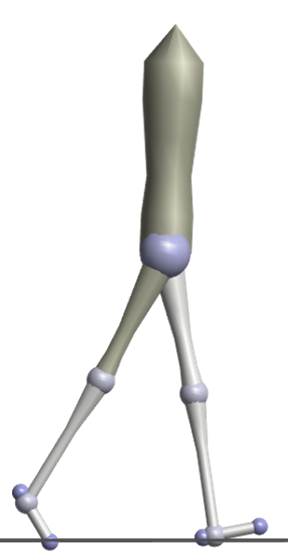
\includegraphics[height=0.3\textheight]{img/7link.png}
%    \caption{The 7-link planar biped model}
%    \label{fig:planar_biped}
%\end{figure}
We also experiment with a 7-link planar 2-dimensional human-like robot model as shown in Figure \ref{fig_nmm}. It has two legs - composed of foot, shin and thigh and a hip. There are 6 actuators at the ankle, knee and hip joints in each leg with infinite allowed torque. This model is used as a simple 2-dimensional approximation to more complex humanoid robots. 

\section{Controllers tested}

\subsection{Neuromuscular model for humanoid robots}

\label{sec:NMC}
We use neuromuscular model policies, as introduced in \cite{geyer2010muscle}, as our controller for a 7-link planar human-like model. These policies use approximate models of muscle dynamics and human-inspired reflex pathways to generate joint torques, producing gaits that are similar to human walking in stance. \cite{desai} designed reflex laws for swing that enable target foot-placement and leg clearance, by analyzing the double pendulum dynamics of the human leg. Integrating this swing control with the previous reflex control enables the model to overcome disturbances in the range of up to $\pm 10 cm$, as described in \cite{song2015neural}. We next describe this control in some detail.

\subsubsection{Neuromuscular Stance Control} 

In stance of the neuromuscular controller, each leg is actuated by 7 Hill-type muscles \cite{morrison1970mechanics}, consisting of the soleus (SOL), gastrocnemius (GAS), vastus (VAS), hamstring (HAM), tibialis anterior (TA), hip flexors (HFL) and gluteus (GLU), illustrated in Figure \ref{fig_nmm}. Together, these muscles produce torques about the hip, knee and ankle. The muscle force $F$ is a non-linear function of the muscle state $s^m$ and stimulus $S^m$, which when multiplied by the moment arm $r(\theta_i)$ gives the resultant torque on joint $i$:
\begin{equation*}
\tau_i^m = F(S^m, s^m)r(\theta_i),
\end{equation*}   
where $\tau_i^m$ is the torque applied by muscle $m$ on joint $i$ and $\theta_i$ is the joint angle.
 
\begin{figure}[t]
    \centering
    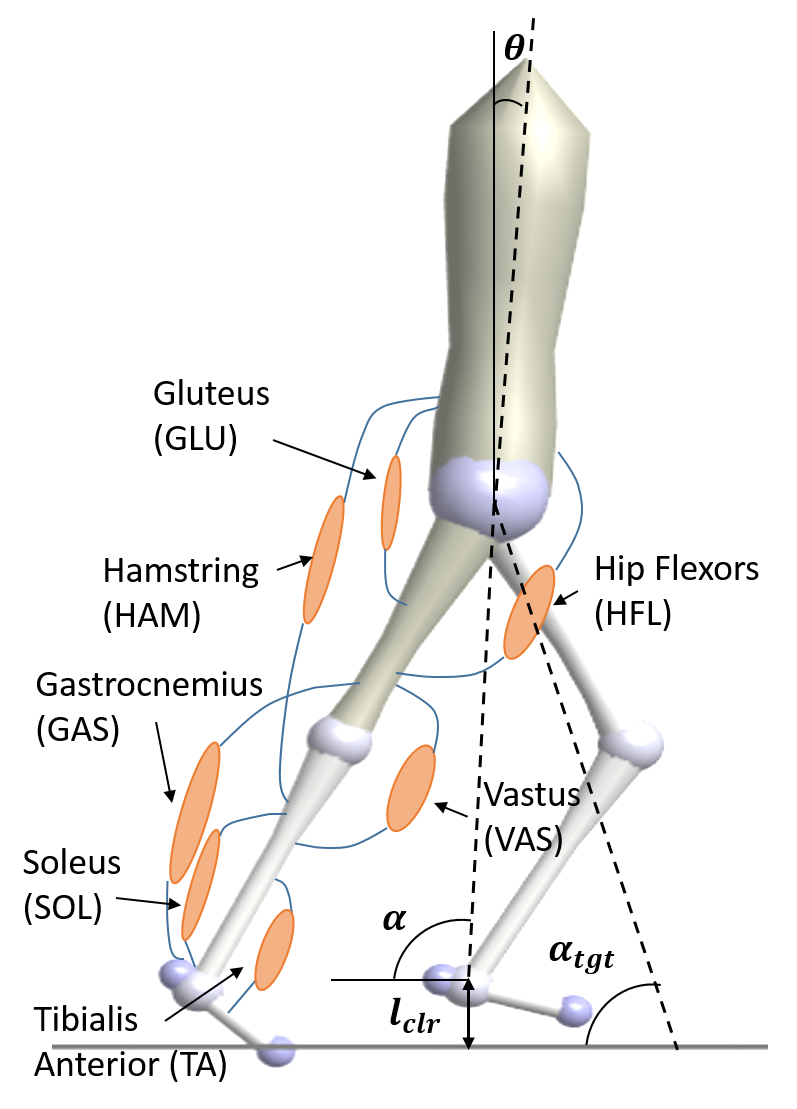
\includegraphics[height=0.3\textheight]{img/nmm_pic.png}
    \caption{The neuromuscular model. The muscles and swing parameters are highlighted.}
    \label{fig_nmm}
\end{figure}

Most of the muscle reflexes in stance are positive length or force feedback on the muscle stimulus. In general, the stimulus $S^m(t)$ for muscle $m$ is a function of the time delayed length or force signal $P^m$ times a feedback gain $K^m$:
\begin{equation*}
S^m(t) =  S_0^m + K^m \cdot P^m(t - \Delta t),
\end{equation*}
where $S_0^m$ is the pre-stimulus, $K^m$ is the feedback gain and $P^m$ is the time-delayed feedback signal of length or force. Some muscles can be co-activated and have multiple feedback signals from more than one muscle. The feedback gains $K^m$ described above are a subset of the parameters that we aim to tune in our optimization. The details of these feedback pathways can be found in \cite{song2015neural}.

This feedback structure generates compliant leg behaviour and prevents the knee from overextending in stance. To balance the trunk, feedback on the torso angle is added to the GLU stimulus:
\begin{equation*}
S^{GLU}_{torso}(t) = K_p^{stance}(\theta_{des} - \theta) -K_d^{stance}\dot{\theta},
\end{equation*}
where $K_p^{stance}$ is the position gain on the torso angle $\theta$ and $\theta_{des}$ is the desired angle. $K_d^{stance}$ is the velocity gain and $\dot{\theta}$ is the angular velocity.
Specifically, here are the stance parameters we optimize over, and their roles in the neuromuscular model:
 
\begin{itemize}
\item $K^{GAS}$ : Positive force feedback gain on GAS
\vspace{-2mm}
\item $K^{GLU}$ : Positive force feedback gain on GLU
\vspace{-2mm}
\item $K^{HAM}$ : Positive force feedback gain on HAM
\vspace{-2mm}
\item $K^{SOL}$ : Positive force feedback gain on SOL
\vspace{-2mm}
\item $K^{TA}_{SOL}$ : Negative force feedback from SOL on TA
\vspace{-2mm}
\item $K^{TA}$ : Positive length feedback on TA
\vspace{-2mm}
\item $K^{VAS}$ : Positive force feedback on VAS
\vspace{-2mm}
\item $K^{stance}_p$ : Position gain on feedback on torso angle
\vspace{-2mm}
\item $K^{stance}_d$ : Velocity gain on feedback on torso velocity
\vspace{-2mm}
\item $K_{mix}^{GLU}$ : Gain for mixing force feedback and feedback on angle for GLU
\end{itemize}

\subsubsection{Swing Leg Placement Control}

The swing control is controlled by three main components -- target leg angle, leg clearance and hip control. Target leg angle is a direct result of the foot placement strategy which is a function of the velocity of the center of mass (CoM) $v$, and the as distance between the stance leg the CoM, and presented in \cite{simbicon}:
\begin{equation*}
\alpha_{tgt} = \alpha_0 + C_d d + C_v v,
\end{equation*}
where $\alpha_{tgt}$ is the target leg angle, $\alpha_0$ is the nominal leg angle, $\alpha_0$, $C_d$ and $C_v$ are parameters optimized by our control.

Leg clearance is a function of the desired leg retraction during swing. The knee is actively flexed until the leg reaches the desired leg clearance height, $l_{clr}$ and then held at this height, until the leg reaches a threshold leg angle. At this point, the knee is extended and allowed to reach the target leg angle $\alpha_{tgt}$. Details of this control can be found in \cite{desai}. As was noted in \cite{song2015neural}, and observed in our experiments, the control is relatively insensitive to the individual gains of the set-up in swing. It is sufficient to control the higher level parameters such as the desired leg clearance and target leg angle.

The third part of the control involves maintaining the desired leg angle $\alpha_{tgt}$ by applying a hip torque $\tau_{hip}^{\alpha}$:
\begin{equation*}
\tau_{hip}^{\alpha} = K_p^{swing}(\alpha_{tgt} - \alpha) - K_d^{swing}(\dot{\alpha}),
\end{equation*}
where $K_p^{swing}$ is the position gain on the leg angle, $K_d^{swing}$ is the velocity gain, $\alpha$ is the leg angle and $\dot{\alpha}$ is the leg angular velocity (see Figure \ref{fig_nmm}). 

More concisely, the swing parameters that we focus on in our optimization are the following:
\begin{enumerate}
\item $K_p^{swing}$ : Position gain on feedback on leg angle
\vspace{-2mm}
\item $K_d^{swing}$ : Velocity gain on feedback on leg velocity
\vspace{-2mm}
\item $\alpha_0$ : Nominal leg angle
\vspace{-2mm}
\item $C_d$ : Gain on the horizontal distance between the stance foot and CoM
\vspace{-2mm}
\item $C_v$ : Gain on the horizontal velocity of the CoM
\vspace{-2mm}
\item $l_{clr}$ : Desired leg clearance
\end{enumerate}

Though originally developed for explaining human neural control pathways, these controllers have recently been applied to robots and prosthetics, for example in \cite{thatte} and \cite{van2015biped}. As demonstrated in \cite{song2015neural}, these models are indeed capable of generating a variety of locomotion behaviours for a humanoid model - for example, walking on flat, rough ground, turning, running, walking upstairs and on ramps. However, a full study of using these models to control biped robots still needs to be done. Whether these models will transfer well to robots with significantly different dynamics and inertial properties than humans needs to be explored. It is difficult to transfer these models to robots because of a large number of interdependent gains that need to be tuned. Typically, this is done using Covariance Matrix Adaptation Evolutionary Strategy \mbox{(CMA-ES)} \citep{hansen2006cma}, an evolutionary algorithm for difficult non-linear non-convex black-box optimization problems. Even though CMA-ES is useful for optimizing non-convex problems in high dimensions, it is not sample efficient and depends on the initial starting point. An optimization for 16 neuromuscular parameters takes 400 generations, around a day on a standard i7 processor and about 5,000 trials, as reported in \cite{song2015neural}. 

The large number of trials make it impossible to implement CMA-ES on a real robot. This is a shortcoming because often we find that after training the policies in simulation, they do not transfer well to the real robot, due to differences between simulation and real hardware. We aim to overcome this problem by using Bayesian Optimization with informed feature transforms for optimizing controllers.
%In the following sections, we will develop a sample efficient method for training the same controller. 

The neuromuscular controller is a model-free controller. It does not need the exact dynamics of the robot to generate torques. The dynamics are inherently embedded in the learned parameters of the controller. As a result, the same controller can be used on very different robots without any modification to the policy structure. We later show a very similar controller implemented on the ATRIAS bipedal robot.

We next describe a model-based reactively stepping controller. This controller uses the dynamics models of the robot to generate torques. Hence, to transfer to new systems, the dynamics need to be updated.


\subsection{Feedback based reactive stepping policy}
\label{sec:raibert_cont}
We design a parametric controller for controlling the CoM height, torso angle and the swing leg by commanding desired ground reaction forces and swing foot landing location. 
\begin{align}
    \label{eq:raibert}
    F_x = K_{pt}(\theta_{des} - \theta) + K_{dt}(\dot{\theta}_{des} - \dot{\theta}) \\
    F_z = K_{pz}(z_{des} - z) + K_{dz}(\dot{z}_{des} - \dot{z})\\
    x_p = k(v-v_{tgt}) + C \cdot d + 0.5 \cdot v \cdot T
\end{align}
Here, $F_x$ is the desired horizontal ground reaction force (GRF), $K_{pt}$ is the proportional gain on the torso angle $\theta$ and $K_{dt}$ is the derivative gain on the torso angular velocity $\dot{\theta}$. $\theta_{des}$ and $\dot{\theta}_{des}$ are the desired torso lean and desired torso angular velocity. $F_z$ is the desired vertical GRF, $K_{pz}$ is the proportional gain on the CoM height $z$ and $K_{dz}$ is the derivative gain on the CoM vertical velocity $\dot{z}$. $z_{des}$ and $\dot{z}_{des}$ are the desired CoM height and desired CoM vertical velocity. Both $\dot{\theta}_{des}$ and $\dot{z}_{des}$ are always set to $0$. $x_p$ is the desired foot landing location for the end of swing; $v$ is the horizontal CoM velocity, $k$ is the feedback gain that regulates $v$ towards the target velocity $v_{tgt}$. These quantities are highlighed in Figure \ref{fig:raibert_com}. $C$ is a constant and $d$ is the distance between the stance leg and the CoM; $T$ is the swing time and the term $0.5 \cdot v \cdot T$ is a feedforward term similar to a Raibert hopping policy, described in \cite{raibert1986legged}.
\begin{figure}[t]
    \centering
    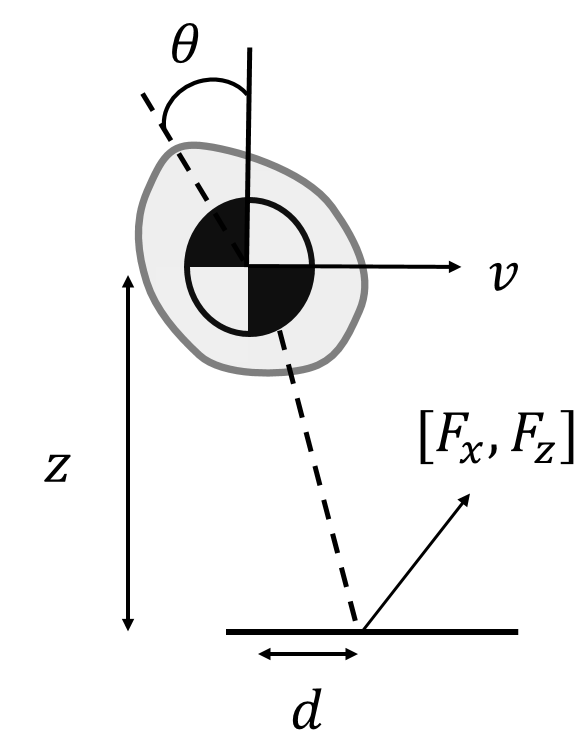
\includegraphics[width=0.3\textwidth]{img/raibert_com.png}
    \caption{\small{Illustration of the Center of Mass model and variables used for the feedback-based stepping policy.}}
    \label{fig:raibert_com}
\end{figure}

This parametrization results in desired ground reaction forces (GRFs) in stance and a desired foot landing position in swing. Note that there is no desired CoM trajectory in this controller. We only command a desired CoM velocity, regulated through the swing foot placement. In stance, the desired GRFs regulate a desired CoM height and torso angle. These are then sent to the ATRIAS inverse dynamics model that generates desired motor torques $(\tau_f, \tau_b)$ that realize the GRFs. 
\begin{equation}
    M \ddot{q} + h = S \tau + J^T F
\end{equation}
where $M$ is the mass matrix, $\ddot{q}$ are the joint accelerations, $h$ are the gravitational terms, $S$ is a selection matrix, $\tau$ are resultant joint torques, $J$ is the contact Jacobian and $F = [F_x, F_z]$ are the desired forces generated in \ref{eq:raibert}. There are no Coriolis terms due to the assumption of massless legs. Details can be found in \cite{wu2014highly}. These desired motor torques are then sent to a low level motor velocity-based feedback loop that generates the desired torques in the robot SEAs. % (Fig \ref{fig:control_flow}). 

In swing, we continually re-generate a 5th order spline that starts from the current position and velocity of the swing leg, $x_{sw}$ and $\dot{x}_{sw}$ and terminates at the desired foot position $x_{fp}$, with ground speed matching (swing leg is at rest with respect to the ground). The desired initial and final point of this spline is continually regenerated based on the current estimate of the swing foot position and velocity, as well as the desired footstep and CoM velocity. This trajectory gives the next desired position and velocity of the swing leg, $x_{sw}^*$, $\dot{x}_{sw}^*$, which is translated to desired joint positions and velocities using the robot kinematics. These are then position-controlled by sending a velocity command to the robot SEAs. % (Fig \ref{fig:control_flow}).

%\begin{figure}[t]
%    \centering
%    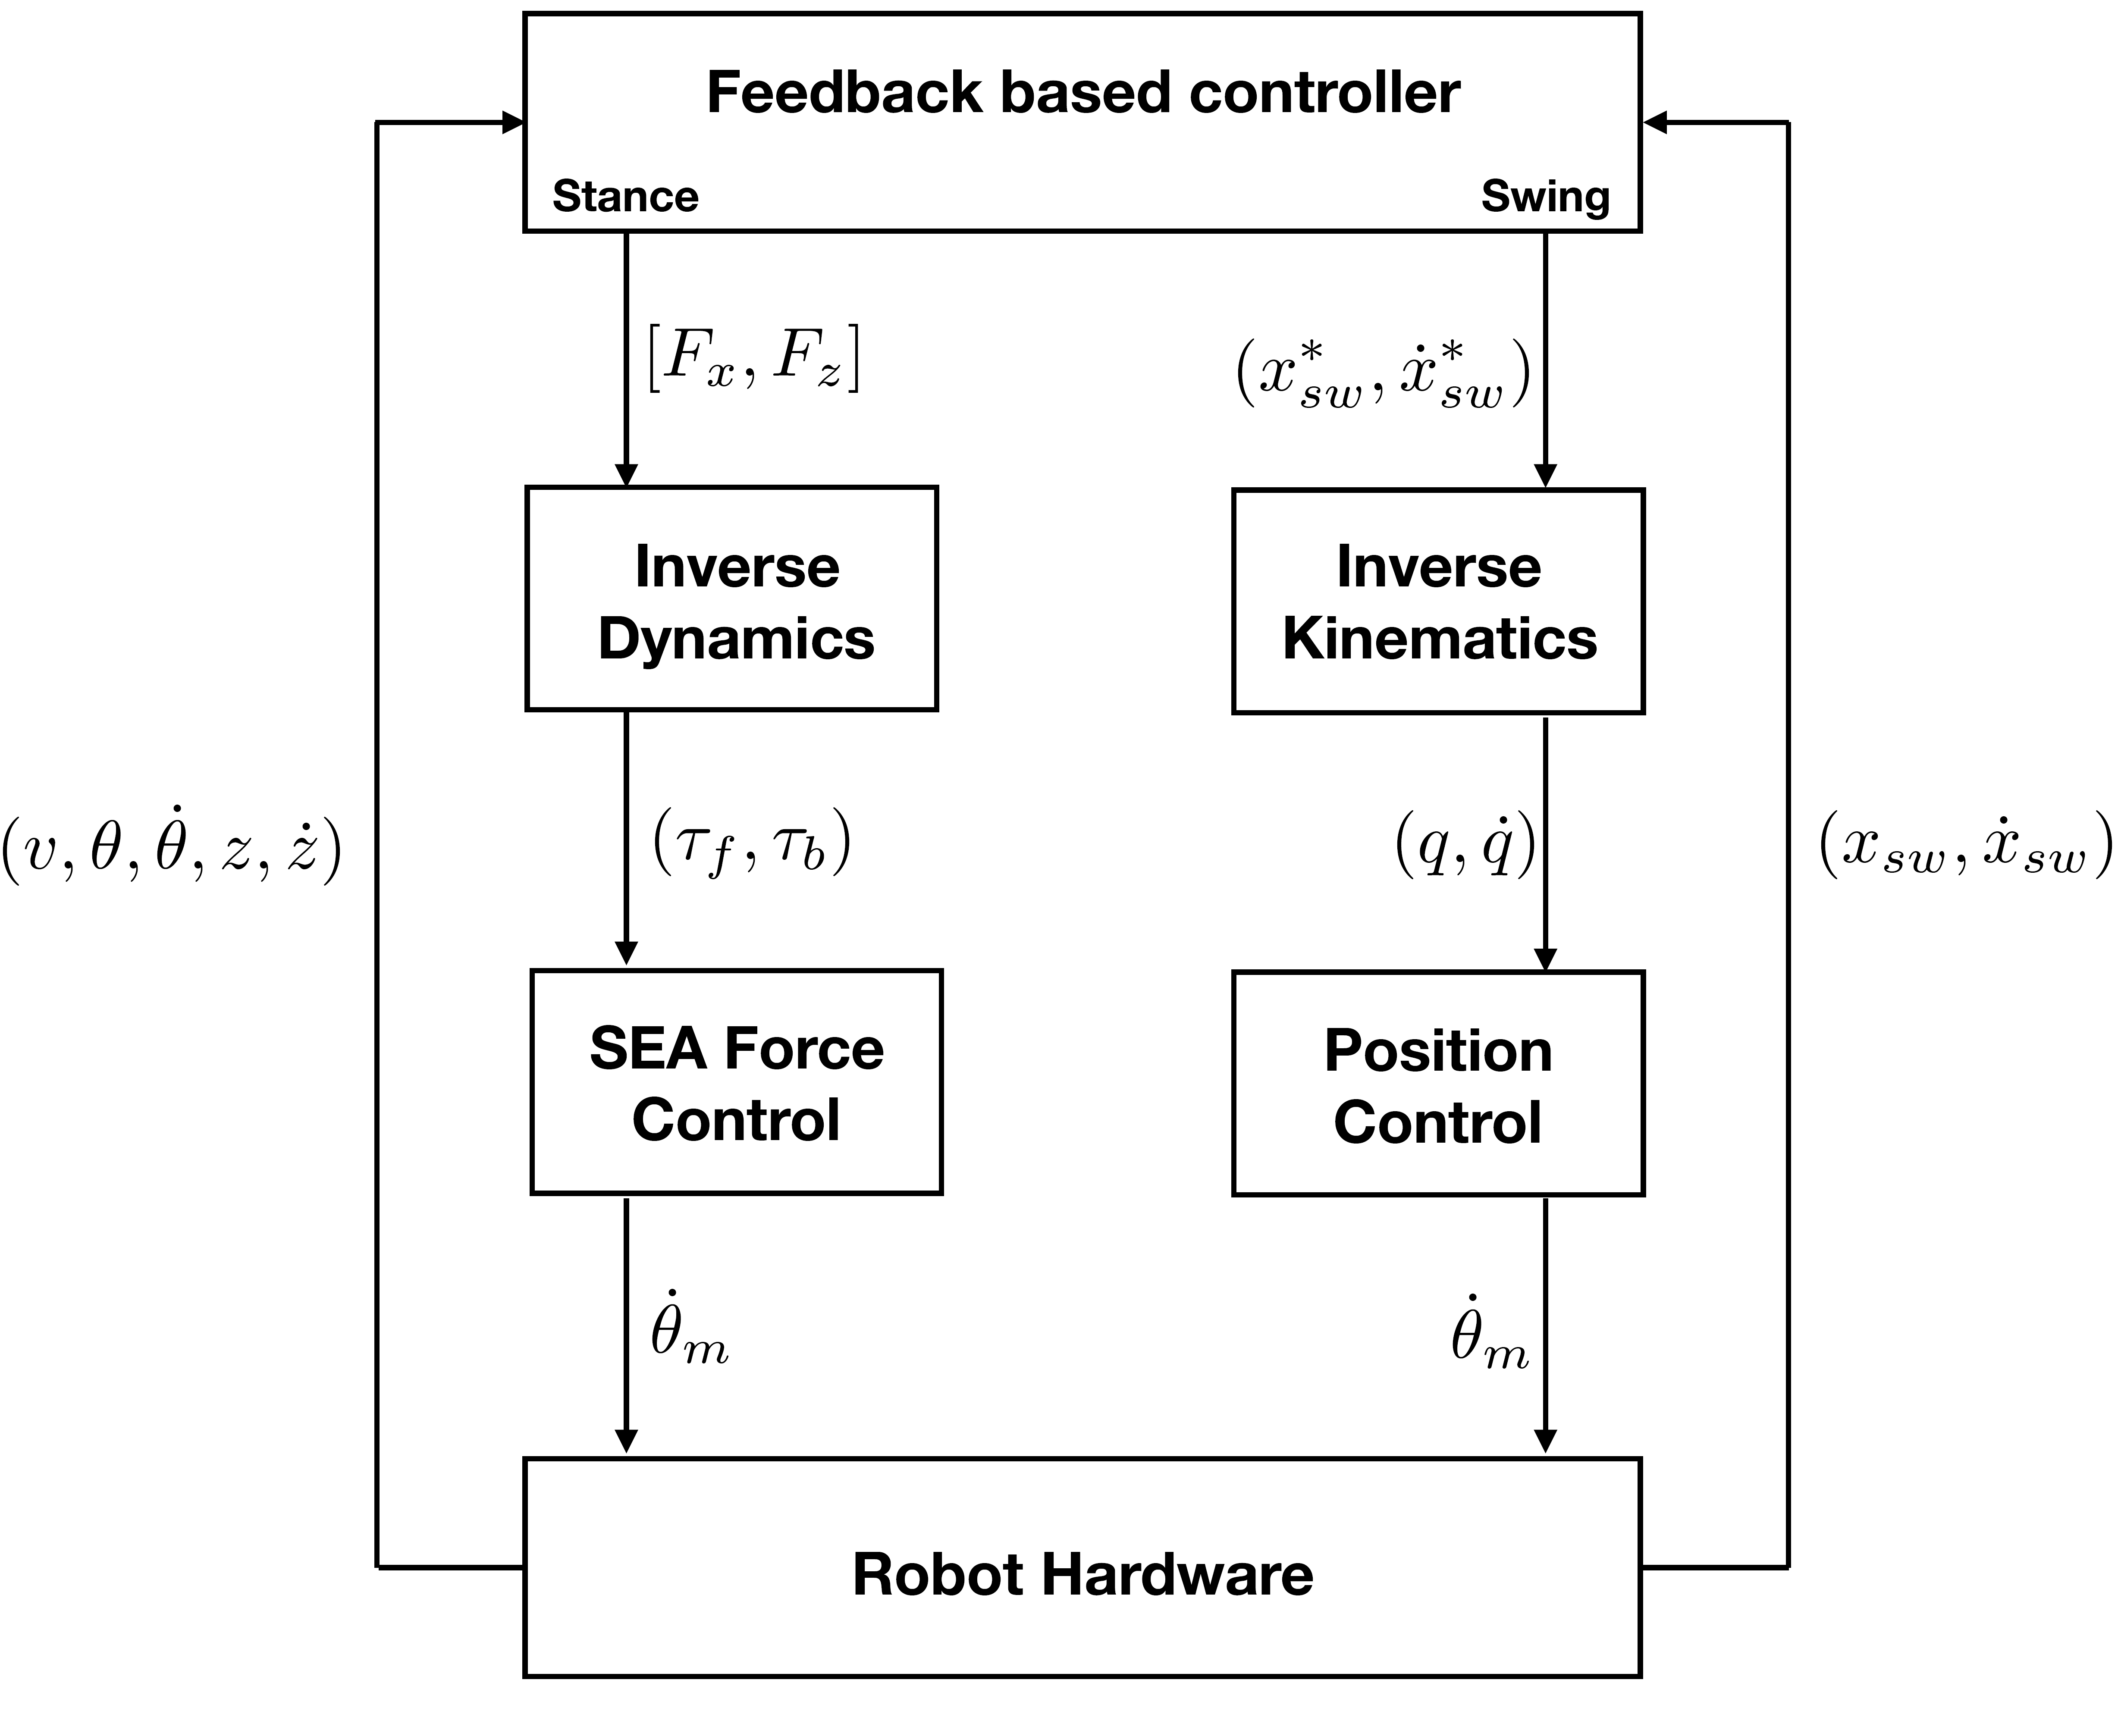
\includegraphics[width=0.8\textwidth]{img/flowchart_cropped.png}
%    \caption{\small{ATRIAS control flowchart with variables from Section~\ref{sec:raibert_cont}}}
%    \label{fig:control_flow}
%\end{figure}

This controller assumes no double-stance, the swing leg takes off as soon as stance is detected. This leads to a highly dynamic gait, as the contact polygon for ATRIAS in single stance is a point. It should be possible to extend this walking controller to include a double stance phase, but we leave that to future work. 

The controller also depends on the desired speed of walking (as this determines the next stepping location). This means that the ``stability" of the controller depends not only on the parameters chosen, but also the desired target speed. We assume that the target speed is provided by the user and is constant in our experiments. It is possible to add the desired speed as an extra dimension to the controller and optimize controllers conditioned on this. But we leave that for future work.

\begin{enumerate}
    \item 5 dimensional walking controller : In our first set of experiments, we optimized 5 parameters from the above described controller. These were $[K_{pt}, K_{dt}, k, C, T]$. The desired positions and velocities were hand tuned, and so was the feedback on $z$.
    \item 9 dimensional walking controller : In our second set of experiments, we optimized 9 parameters of the above described controller. They were :
    
    $[K_{pt}, K_{dt}, \theta_{des}, K_{pz}, K_{dz}, z_{des}, k, C, T]$
\end{enumerate}

\subsection{Virtual Neuromuscular Controller for ATRIAS}
\label{sec:VNMC_cont}

% P1 - summary
We adapt a previously proposed virtual neuromuscular controller (VNMC) \cite{batts2015toward} adapted for ATRIAS. VNMC maps a neuromuscular model to the robot's topology and emulates it to generate desired motor torques, which is sent to the SEA controller (Figure \ref{fig:VNMC}).
The emulated neuromuscular model, which is originally developed to study human locomotion, consists of primarily spinal reflexes, and with appropriate sets of control parameters, it generates diverse human locomotion behaviors \cite{song2015neural}, such as walk, run,turn, walk up stairs, etc. The VNMC control consists of 6 muscles on each leg - the hip flexors (HFL), the glutei (GLU), the hamstrings (HAM), the rectus femoris (RF), the vastii (VAS) and the biceps femoris (BFSH). Since ATRIAS doesn't have any ankles, these muscles are removed from the model. The feedbacks are similar to the ones described in \ref{sec:NMC}, and details can be found in \cite{song2015neural}.

\begin{figure}[t]
\centering
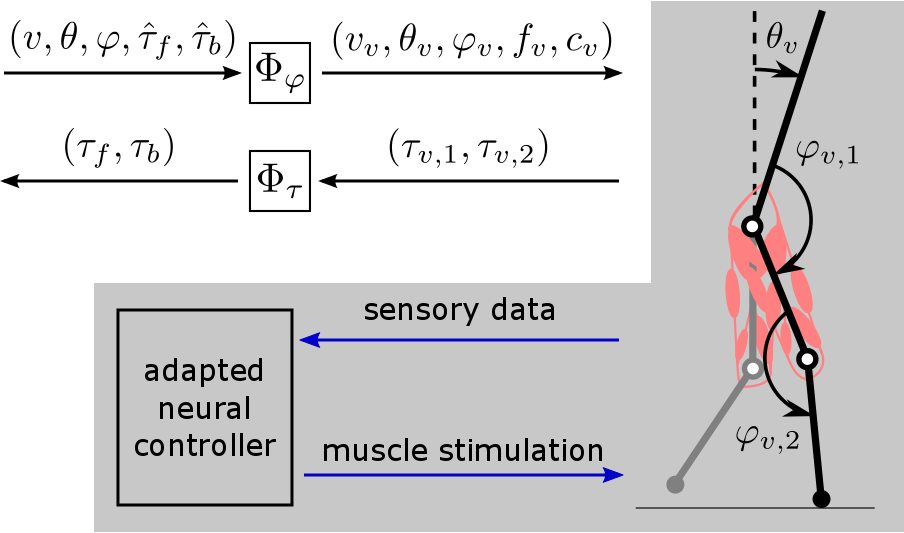
\includegraphics[width=0.6\textwidth]{img/VNMC.png}
\caption{\small{Virtual neuromuscular control.
VNMC maps the robot's state, $(v, \theta, \varphi, \hat{\tau}_f, \hat{\tau}_b)$, to virtual measurements required to emulate a neuromuscular model, $(v_v, \theta_v,  \varphi_v, f_v, c_v)$, where $\varphi$ are joint angles, and $f_v$ and $c_v$ are force and contact data of the virtual leg.
The virtual neuromuscular model (in the gray box) outputs virtual joint torques, $(\tau_{v,1}, \tau_{v,2})$, that are mapped to desired robot joint torques, $(\tau_f, \tau_b)$, which are tracked by the SEA controller.}}
\label{fig:VNMC}
\end{figure}

% P2 - improvements from previous version
For this study, we adapt the previous VNMC \cite{batts2015toward} by removing some unnecessary biological components while preserving its basic functionalities.
First, the new VNMC directly uses joint angular and angular velocity data instead of estimating it from physiologically plausible sensory data, such as muscle fiber states, when applicable.
Second, most of the neural transmission delays are removed, except the ones utilized by the controller.

The adapted VNMC consists of 50 control parameters including feedback gains for each muscle feedback in swing and stance, pre-stimulations for each muscle in swing and stance, high level leg placement gains and desired trunk inclination. When optimized using covariance matrix adaptation evolution strategy \cite{hansen2006cma}, it can control ATRIAS to walk on rough terrains with height changes of $\pm$20 cm in planar simulation. The original VNMC in \cite{batts2015toward} doesn't start from rest, which is impossible to achieve on a robot. To overcome this problem, for now, we start with a 5-dimensional walking controller that can start from rest. Once a desired speed if reached, we switch to the virtual neuromuscular control.

\section{Inaccurate simulations for constructing kernels}

To compare the performance of different methods that can be used to transfer information from simulation to hardware, we create a series of increasingly approximate simulators. These simulators emulate increasing mismatch between simulation and hardware and its effect on the information transfer. Commonly seen discrepancies between simulation and hardware can be classified into three categories: incorrect dynamics parameters, incorrect dynamics models and incorrect environment/task. Incorrect dynamics parameters include discrepancies such as wrong mass, inertia, CoM location of links of the robot. Incorrect models on the other hand are more systematic errors, such as incorrect friction models, actuator dynamics and unmodeled parts of the robot. The third type of discrepancy occurs when simulation is modelling a task different from what is seen on hardware, for example walking on flat ground vs climbing stairs.  We perturb our simulation to create discrepancies of the first two kinds described above, and test the performance of BO at optimizing a 5, 9 and 50 dimensional controller. This allows us to study the effect of increasing mismatch between simulation and hardware on the performance of our proposed approach.

\subsection{Incorrect dynamics parameters}
Our first set of experiments create a  \textit{``simulated hardware"} that is increasingly different from the simulation, in which the DoG features were collected. This is done by changing the mass, inertia, center of mass location of each link of the  by up to $\pm x\%$ ($x = 20, 40, 60$) of its original value. This perturbed simulation now serves as a test hardware for features calculated in the unperturbed simulator. The friction coefficient of the ground contact models, ground stiffness and actuator delay is also changed by the same amount. 
Unlike domain-randomization, from \cite{mordatch2015ensemble}, instead of training on perturbations, we test on these perturbations. This setup is designed to test whether our approach can be used even when the scale of mismatch between simulation and hardware is unknown a-priori.

\subsection{Incorrect dynamics models}
In this setting, the high-fidelity ATRIAS simulator~\citep{martin2015robust}, is the \textit{simulated ``hardware"}. We make dynamics approximations to the original simulator, which are used commonly in simulators to decrease fidelity and increase simulation speed. For example, the complex dynamics of harmonic drives are approximated as a torque multiplication, and the boom is removed from the simulation, leading to a two-dimensional simulator. These approximate simulators now become the \textit{simulated ``simulators"}. As the approximations in these simulators are increased, we expect the performance of methods that utilize simulation for optimization on hardware to deteriorate.

\begin{figure}
    \centering
    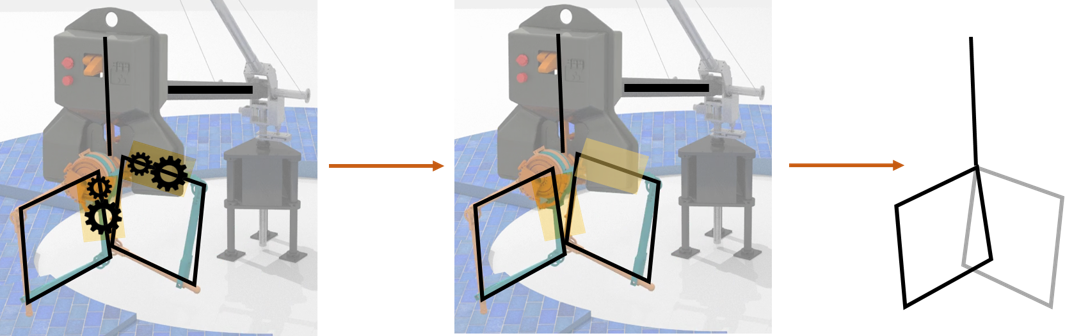
\includegraphics[width = 0.8\textwidth]{img/atrias_gear_boom_simplification.png}
    \caption{Different fidelity simulators for ATRIAS. The original simulator (left) is very high-fidelity with complex gear and boom dynamics. The second simulator (middle) has an approximate gear dynamics model and the third simulator (right) simulates a 2-dimensional robot without boom or gear dynamics.}
    \label{fig:simulators}
\end{figure}

The details of the approximate simulators are described below:

\begin{enumerate}
    \item \textbf{Simulation with simplified gear dynamics} : The ATRIAS robot has geared DC motors attached to leaf springs on the legs. Their high gear ratio of 50 is achieved through a harmonic drive. In the original simulator, this drive is modelled using gear constraints in MATLAB SimScape Multibody simulation environment. These require significant computation time as the constraint equations have to be solved at every time instant, but lead to a very good match between the robot and simulation. We replace this model with a commonly used approximation for geared systems -- multiplying the rotor torque by the gear ratio. This reduces the simulation time to about a third of the original simulator, but leads to an approximate gear dynamics model.

    \item \textbf{Simulation with no boom and simplified gear dynamics} : The ATRIAS robot walks on a boom in our hardware experiments. The boom leads to lateral torques on the robot, which have vertical and horizontal force components that need to be considered in a realistic simulation of the robot. In our second approximation, we remove the boom from the original simulator and constraint the motion of the robot to a 2-dimensional plane, making a truly two-dimensional simulation of ATRIAS. This is a common approximation for two-dimensional robots. Since this approximation has both simplified gear dynamics and no boom, it is further from the original simulator than the first approximation.

\end{enumerate}

A visual illustration of these approximations is shown in Figure \ref{fig:simulators}. The advantage of such an arrangement is that we can extensively test the effect of un-modelled and wrongly modelled dynamics on information transfer between simulation and hardware. Even in our high-fidelity original simulator, there are several un-modelled components of the actual hardware. For example, the non-rigidness of the robot parts, misaligned motors and relative play between joints. In our experiments, we find that the 50-dimensional VNMC is a sensitive controller, with little hope of directly transferring from simulation to hardware. Anticipating this, we can now test several methods of compensating for this mismatch using our increasingly approximate simulators. In the future, we would like to take this approximations further and study when there is useful information even in over-simplified simulations of legged systems.


 
\chapter{Experiments with feature transforms from simulation}


We now present our experiments to evaluate the different ways of transferring information from simulation to hardware described in the previous sections. We start by describing hardware experiments with feature transforms, followed by simulation experiments that study the effect of inaccurate simulations. 

%\section{Experiments}

Our key experiments with the domain-specific feature transform and the data-driven feature transform are conducted on the ATRIAS robot. We also include experiments on a 7-link biped in simulation. 

The experiments described in this Section are:
\begin{itemize}
    \item Hardware experiments learning parameters of a feedback-based reactively stepping controller - optimizing 5 and 9 parameters 
    \item Simulation experiments on a neuromuscular controller for humanoid robots - optimizing 16 parameters of the controller
    \item Simulation experiments with a 50-dimensional virtual neuromuscular controller for the ATRIAS robot -  studying the effect of deteriorating simulation on performance
\end{itemize}

\section{Experiments with the DoG Transform}

\subsection{Hardware experiments with the 5-dimensional controller}
\label{sec:hdw_5d}
The first set of hardware experiments were conducted on a 5-dimensional controller, described in Section~\ref{sec:raibert_cont} on the ATRIAS robot. The target speed profile for these experiments was $0.4 m/s \text{ (15 steps)} - 1.0 m/s \text{ (15 steps)} - 0.2 m/s \text{ (15 steps)} - 0 m/s \text{ (5 steps)}$. The total number of steps before the controller shut off were $50$. The cost function that was optimized was:
\begin{equation}
    \label{eq:hdw_cost}
    cost = 
    \begin{cases}
		100 - x_{fall} , \text{\small{if fall}} \\
		||v_{avg} - v_{tgt}||, \text{\small{if walk}}\\
	\end{cases}
\end{equation}

where $x_{fall}$ is the distance in meters covered before falling, $v_{avg}$ is the average speed per step and $v_{tgt}$ is the target velocity profile in $m/s$. 

Random sampling is an effective way of determining how difficult or easy a particular problem is. If random sampling can easily stumble upon successful solutions, the optimization has to be very sample-efficient and reliable to justify the added computational cost. As noted in \cite{calandra2016bayesian}, random sampling often performs better than optimization methods like gradient descent in higher dimensions. 

We sampled 100 random 5-dimensional controllers on hardware and 10 of them walked for this target speed profile. This means that random sampling has a 1/10 chance of sampling a good point. In simulation, 276 points out of 1000 randomly sampled points walked, implying a 1/4 success rate. This highlights the difference between hardware and simulation, making this a tougher problem on hardware.

\begin{figure}[t]
\centering
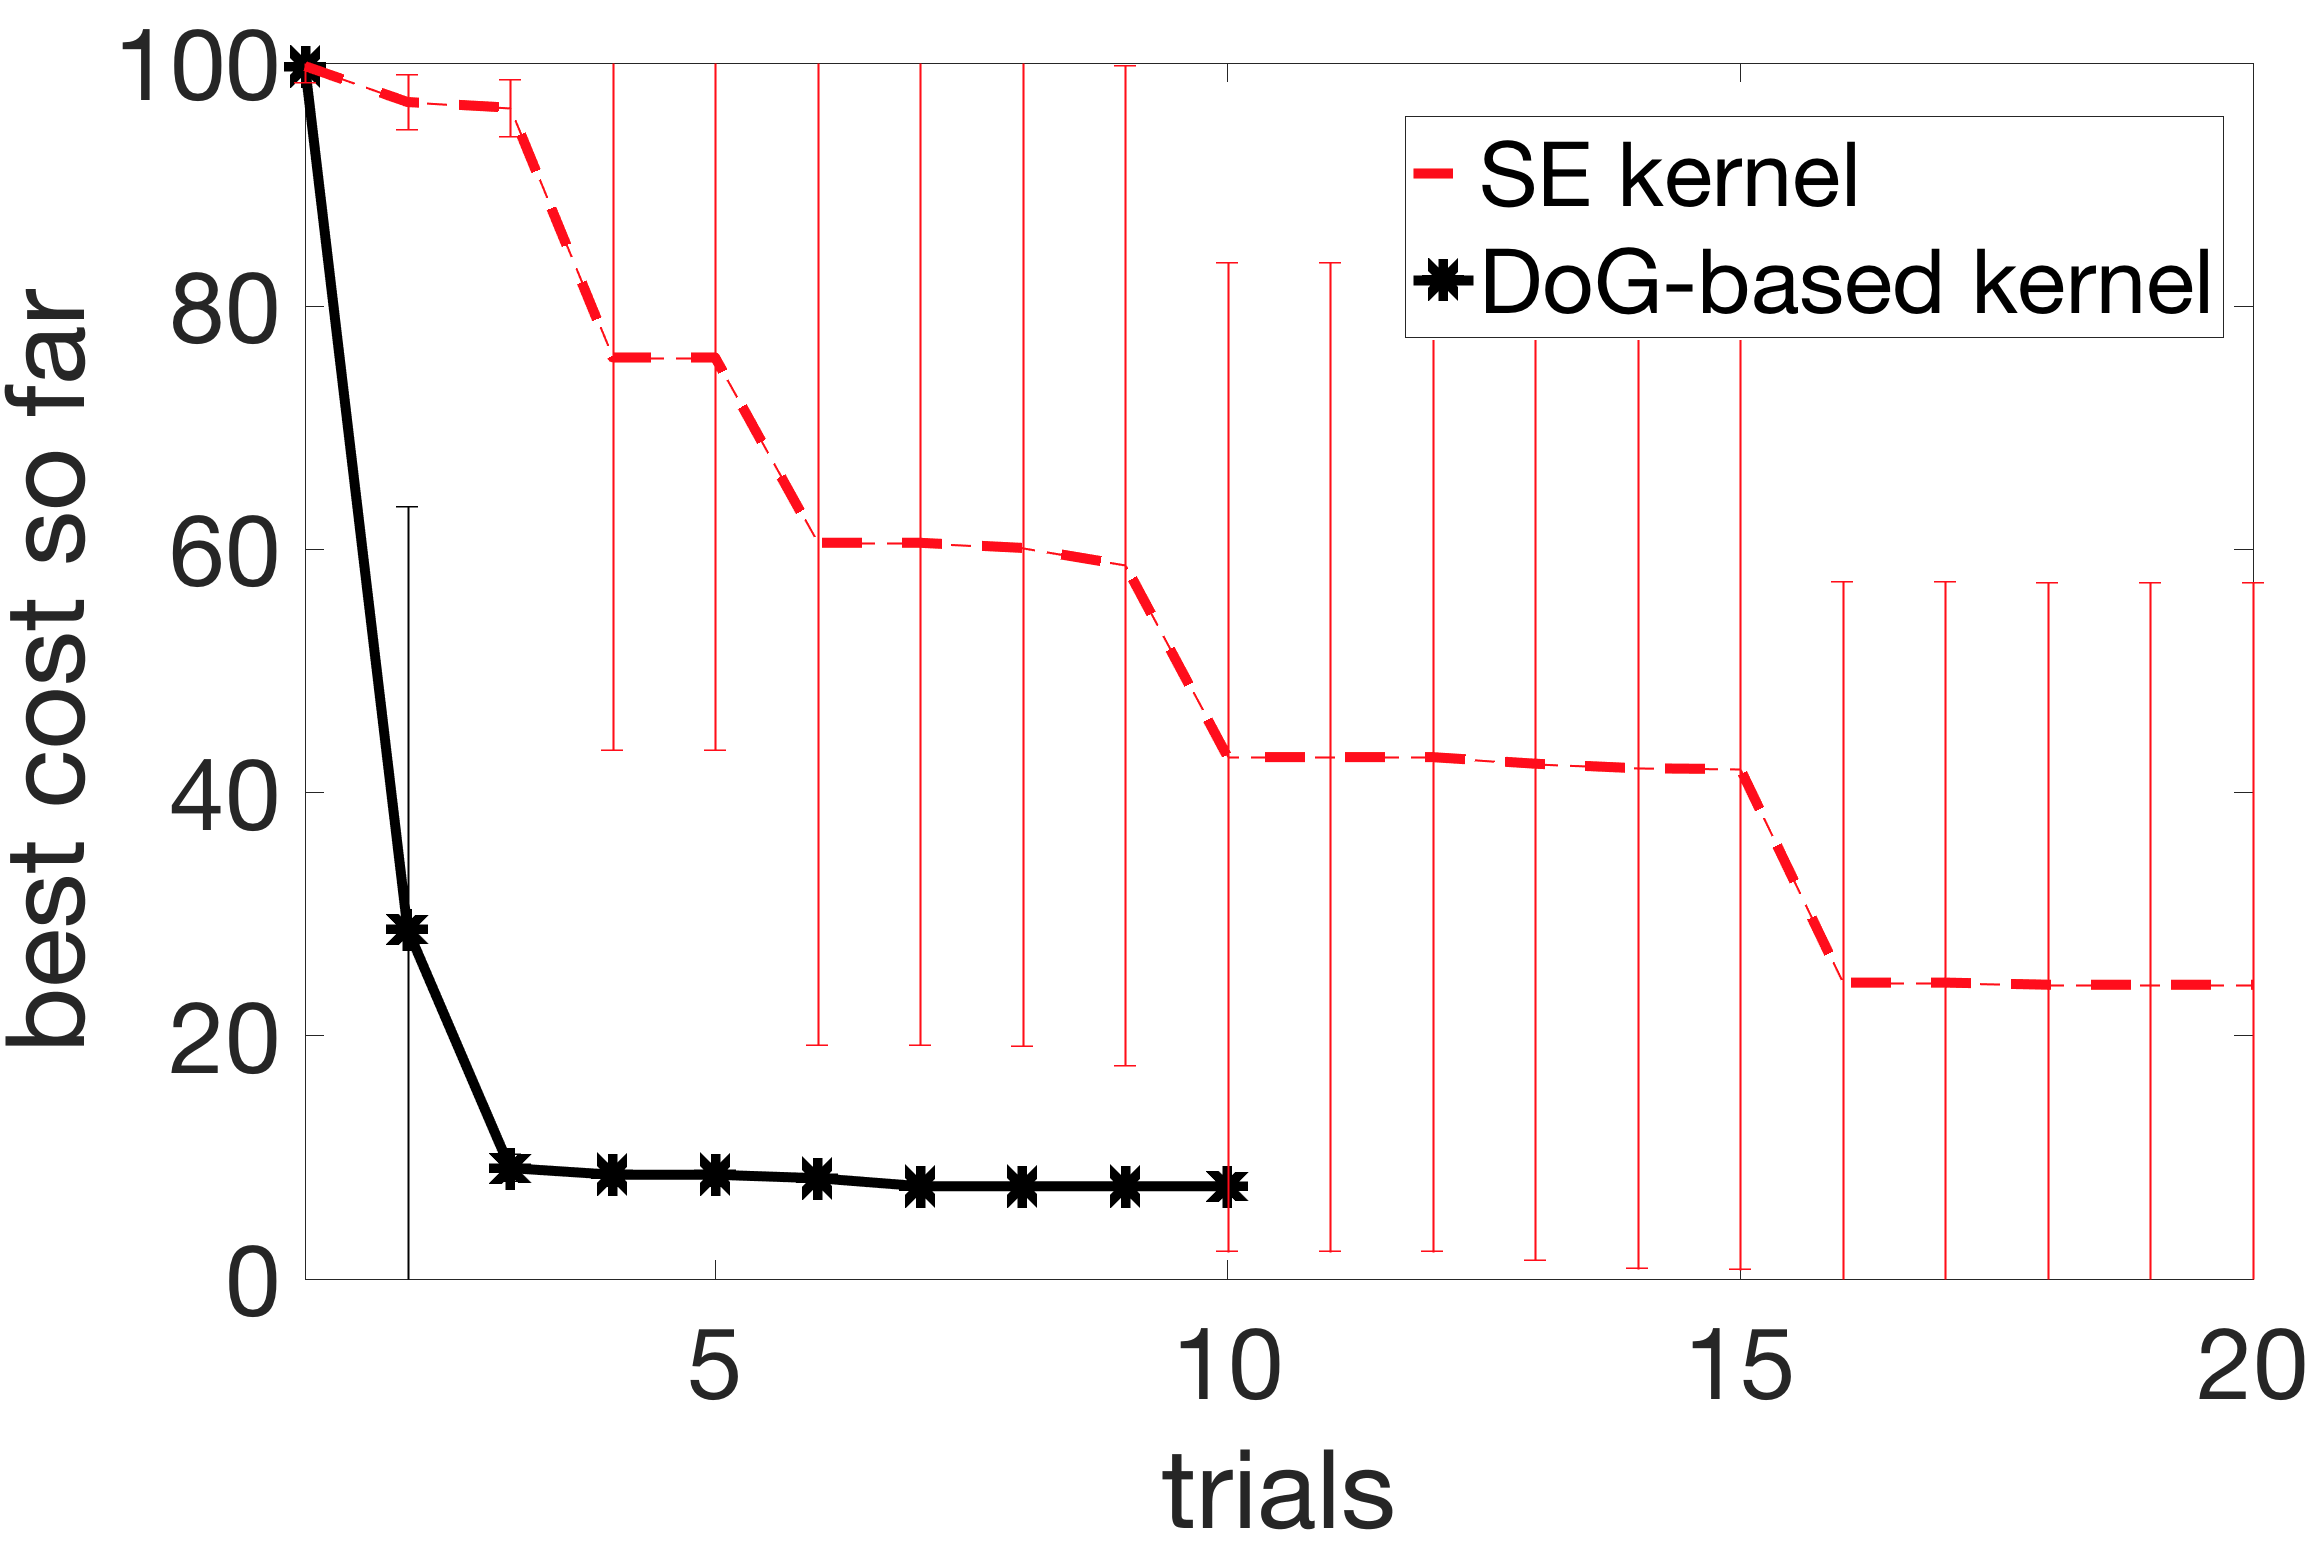
\includegraphics[width=0.6\textwidth]{img/hw_raibert_5d.png}
\caption{\small{BO for 5 dimensional controller on ATRIAS robot hardware. BO with SE finds walking points in 4/5 runs in 20 trials. BO with \dogkernel finds walking points in 5/5 runs in 3 trials.}}
\label{fig:hw_raibert_5d}
\end{figure}

On hardware, we conducted 5 runs of each -- BO with \dogkernel and BO with SE, 10 trials for \dogkernel per run, and 20 for SE kernel. In total, this led to 150 experiments on the robot (excluding the 100 random samples). We also experimented with using fixed vs automatically learned hyperparameters for both kernels. A simple choice of fixed hyperparameters worked well for \dogkernel, while for SE kernel it was better to learn these automatically. DoG scores were calculated on 20,000 points in simulation, by running $3.5s$ long simulations with target speed of $0.5m/s$.

BO with \dogkernel found walking points in 3 trials in 5/5 runs. BO with SE found walking points in 10 trials in 3/5 runs, and in 4/5 runs in 20 trials. These results can be seen in Figure \ref{fig:hw_raibert_5d}.

%\begin{figure}[b]
%\centering
%
\includegraphics[width=0.4\textwidth]{img/TODO.png}
%\caption{\small{Target speed profile and speed of the robot during a trial run on hardware. TODO: modify caption as needed}}
%\label{fig:bo_runs_atrias_hw_slides}
%\end{figure}

%-----------------------------------------------------
\subsection{Hardware experiments with the 9 dimensional controller}
The second set of hardware experiments were conducted on a 9-dimensional controller, described in Section \ref{sec:raibert_cont} on the ATRIAS robot. The target speed profile for these experiments was $0.4 m/s \text{ (30 steps)}$. The total number of steps before the controller shut off was $30$. The cost optimized was the same cost as in Equation \ref{eq:hdw_cost}. 

Again, we sampled 100 random points on hardware and 3 of them walked for this speed profile. This means that random sampling has a 1/33 chance of sampling a good point. On the variable speed profile from Section \ref{sec:hdw_5d}, the number of successful points out of 100 were 0, implying a less than 1\% success rate. To keep the problem at hand reasonable, we used the simpler target speed profile. In comparison, the success rate in simulation is 8\% for the tougher profile, implying a greater mismatch between hardware and simulation than the 5-dimensional controller. 

For this setting, we conducted 3 runs of each BO with \dogkernel and BO with SE, 10 trials for \dogkernel per run, and 10 for SE. In total, this led to 60 experiments on the hardware (excluding the random sampling). 

\begin{figure}[t]
\centering
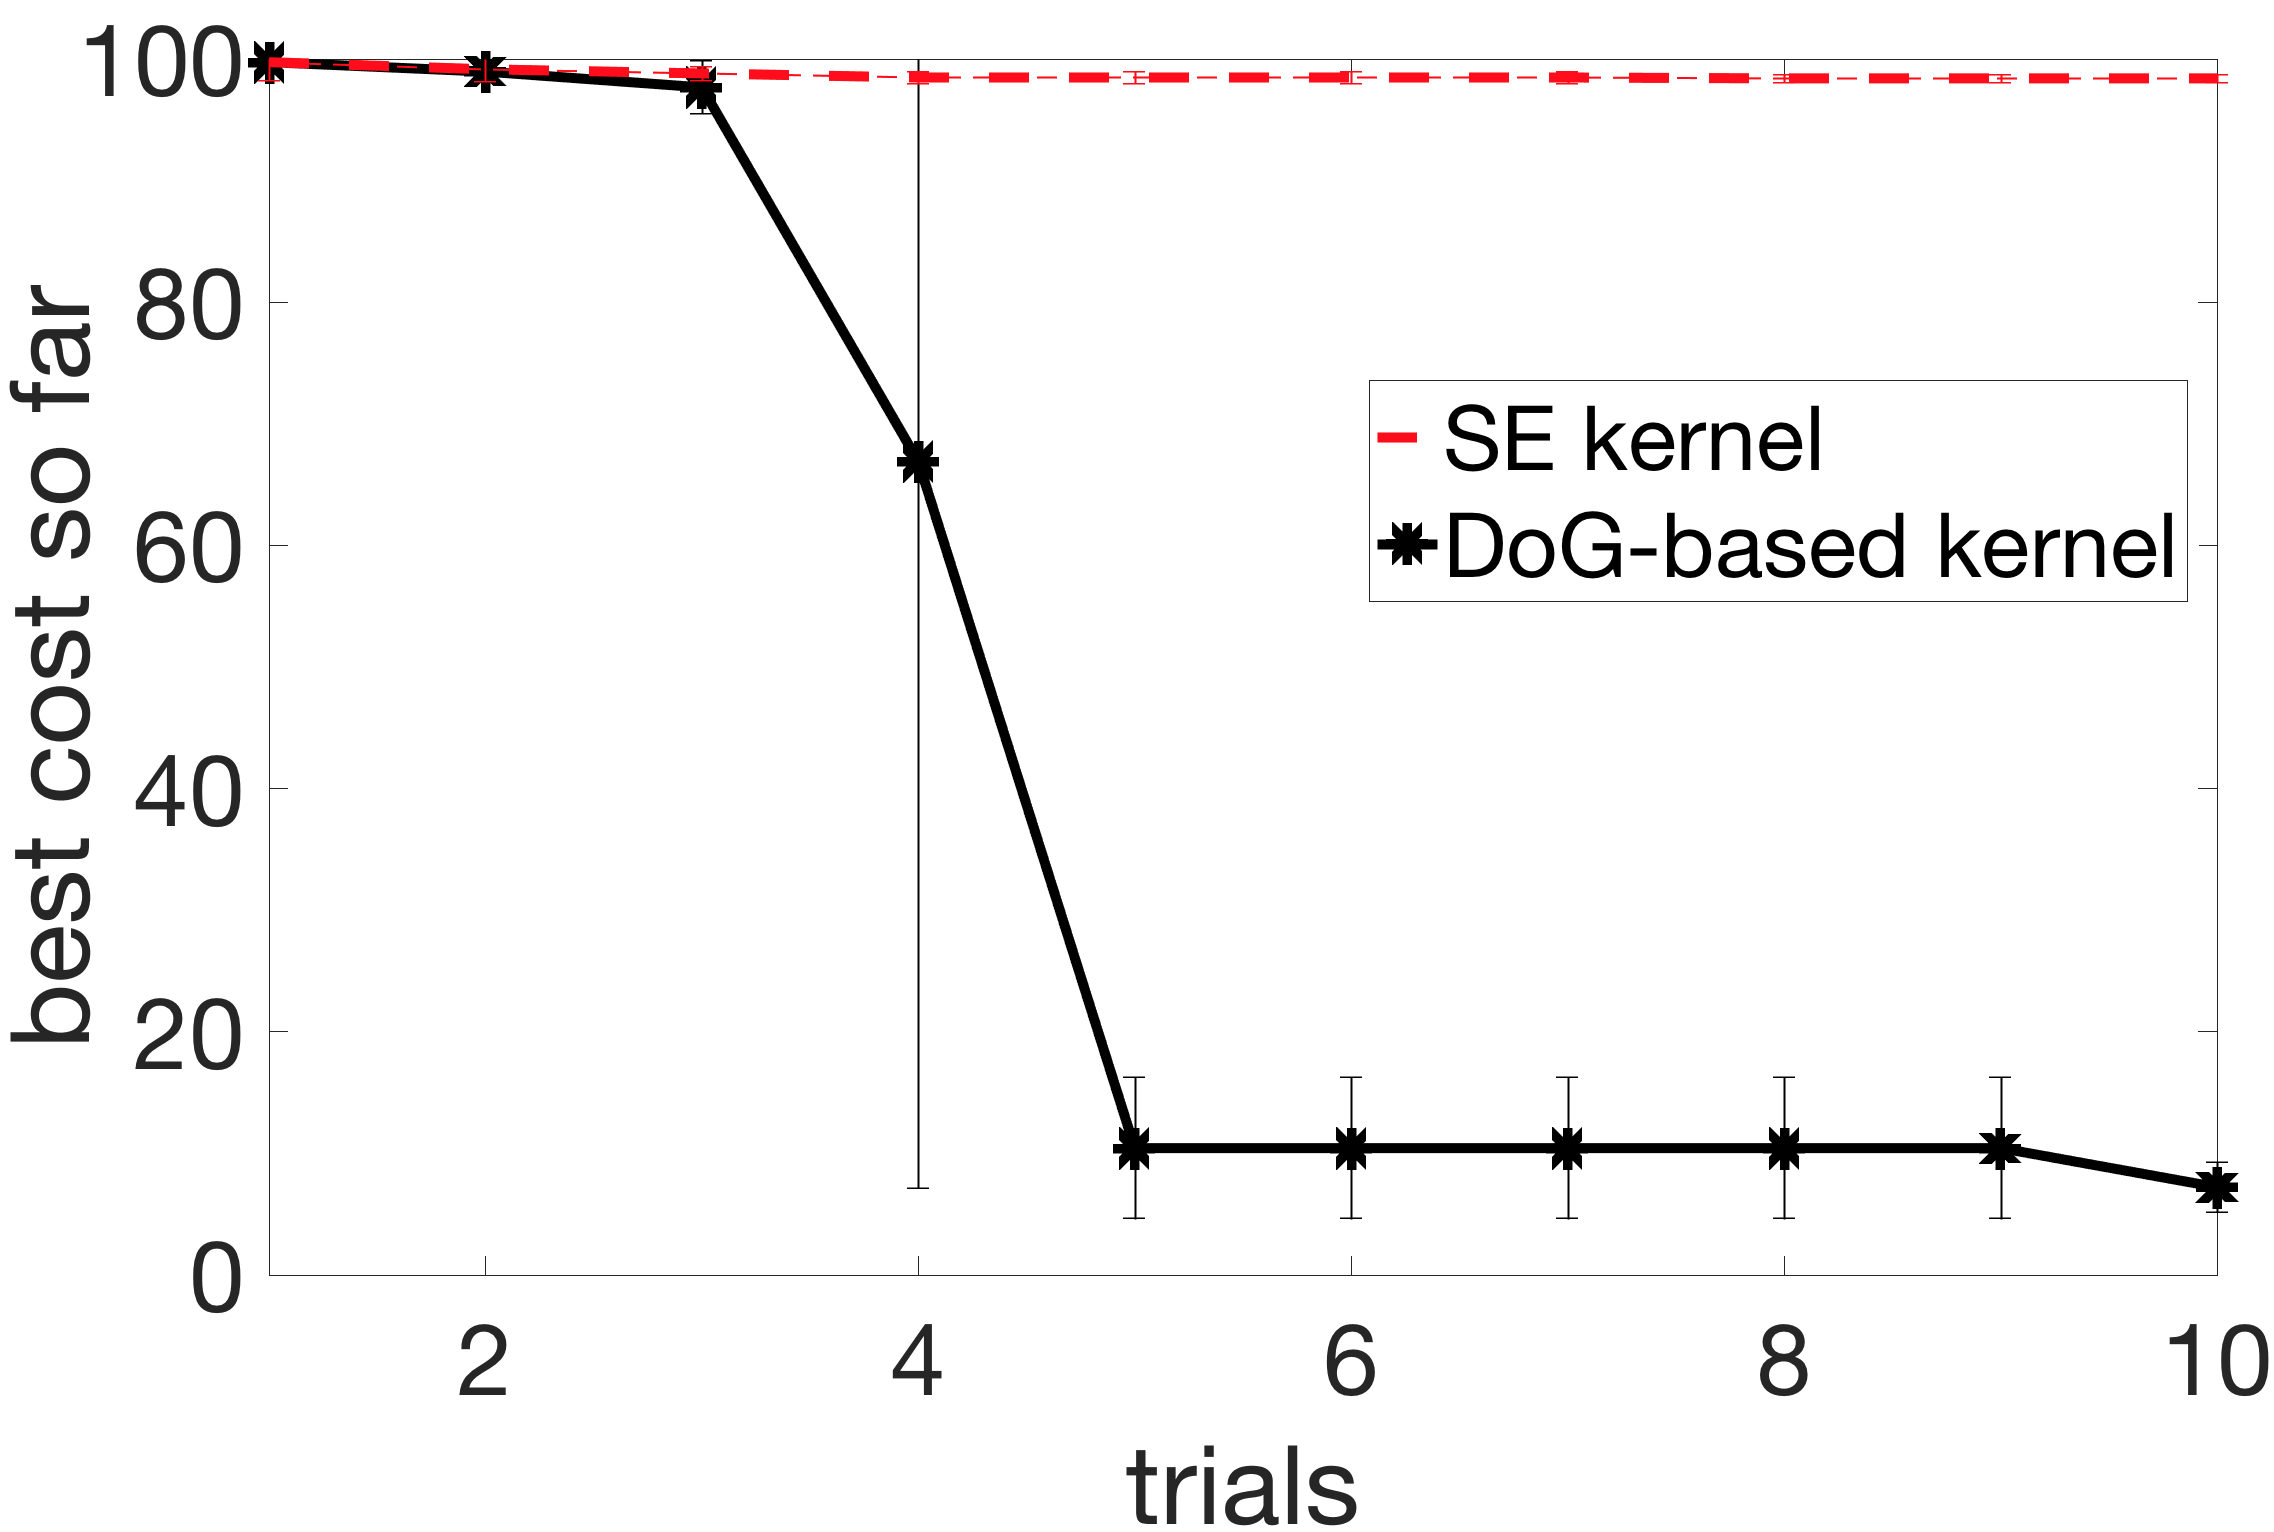
\includegraphics[width=0.6\textwidth]{img/hw_raibert_9d.png}
\caption{\small{BO for 9 dimensional controller on ATRIAS robot hardware. BO with SE doesn't sample any walking points in 3 runs. BO with \dogkernel finds walking points in 5 trials in 3/3 runs.}}
\label{fig:hw_raibert_9d}
\end{figure}

BO with \dogkernel found walking points in 5 trials in 3/3 runs. BO with SE did not find any walking points in 10 trials in all 3 runs. These results can be seen in Figure \ref{fig:hw_raibert_9d}.

Based on these results, we concluded that BO with \dogkernel was indeed able to extract useful information from simulation and speed up learning on hardware. However, it took slightly longer to find points for the 9-dimensional controller and the quality of solution might have improved further if we continued the optimization. This is all as per expectation, as a higher dimensional controller should take longer to optimize, but eventually lead to a better or as good a solution as a smaller dimensional controller. 

\begin{figure}
\centering
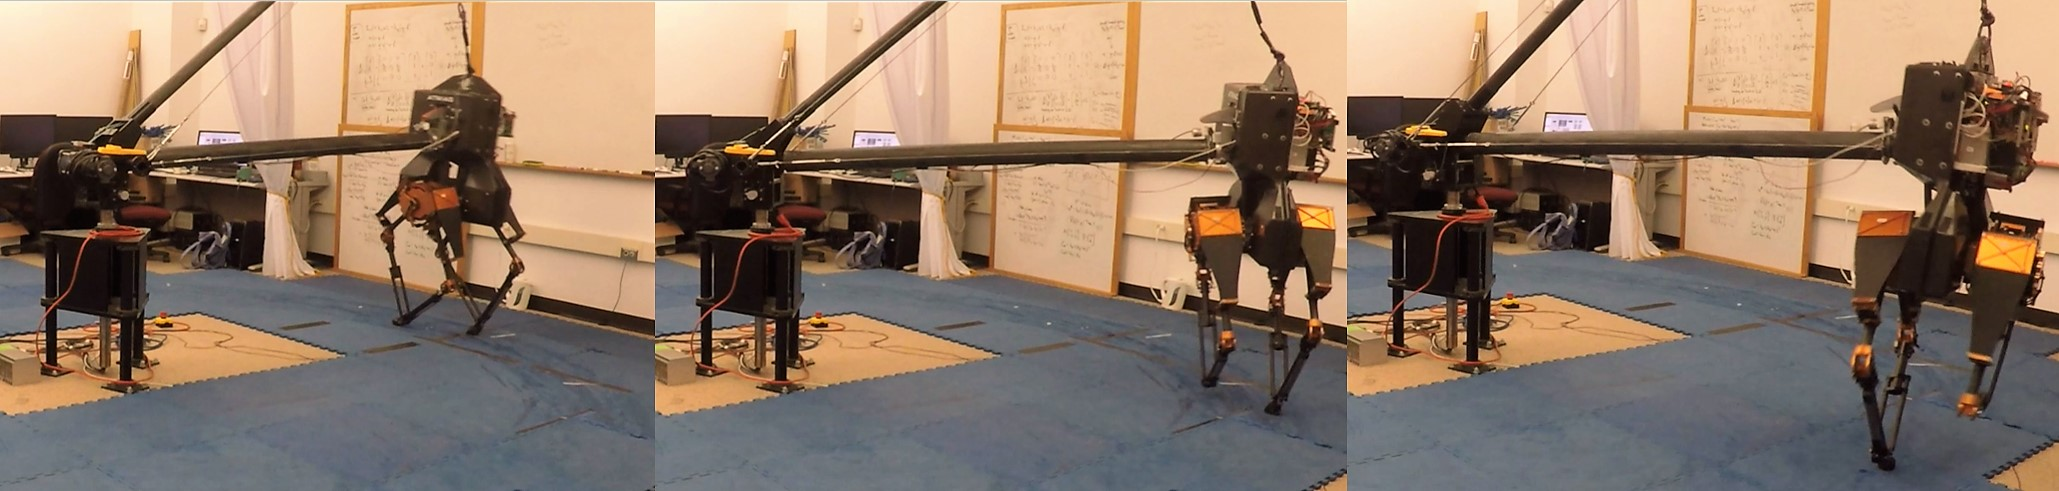
\includegraphics[width=0.98\textwidth]{img/atrias_time_lapse.jpg}
\caption{\small{A time lapse of ATRIAS walking around the boom during a run of \dogkernel.}}
\label{fig:bo_runs_atrias_hw_slides}
\end{figure}


\subsection{Simulation experiments with the 9-dimensional controller}

\label{sec:exps_sim}

To facilitate further experiments we used the ATRIAS simulator from ~\cite{martin2015robust} with modeling disturbances and a variable target speed profile of $0.4 m/s \text{ (15 steps)} - 0.6 m/s \text{ (15 steps)} - 1.0 m/s \text{ (15 steps)} - 0.6 m/s \text{ (15 steps)} - 0.2 m/s \text{ (5 steps)}$. For these experiments, we use the 9-dimensional controller described in \ref{sec:raibert_cont} as this proved to be a more challenging setting for the ATRIAS hardware. Masses of the robot torso, legs, the boom, as well as inertia of the torso were perturbed randomly by up to 15\% of their original values during optimization. This ensured a mismatch between the setting used to generate the kernel and the experimental setting for evaluating its performance, aimed at capturing the discrepancy between hardware and simulation. Note that the kernel was generated on the unperturbed setting, with parameters as described in Section \ref{sec:atrias} for a target speed of $0.5m/s$. The grid size for DoG scores was 100,000 points, and simulations were run for $5s$.

The cost used for these experiments was
\begin{equation}
\label{eq:cost_sim}
cost = 		
    \begin{cases}
		100 - x_{fall} , \text{\small{if fall}} \\
		||v_{avg} - v_{tgt}|| + c_{tr}, \text{\small{if walk}}\\
	\end{cases}
\end{equation}

where $x_{fall}$ is the distance covered before falling in meters, $v_{avg}$ is the average speed per step, $v_{tgt}$ is the target velocity for that step in $m/s$, and $c_{tr}$ captures the cost of transport - calculated by taking a sum of motor torques and normalizing them by a constant. Simulations for evaluating the cost were run for $30s$. Note the addition of the cost of transport in this cost, as compared to \ref{eq:hdw_cost}. $c_{tr}$ needs more than 10 trials to be optimized significantly, and the current low-level motor controllers in Section \ref{sec:raibert_cont} are not designed to reduce $c_{tr}$. Hence, its not considered in the hardware experiments.

\begin{figure}[t]
\centering
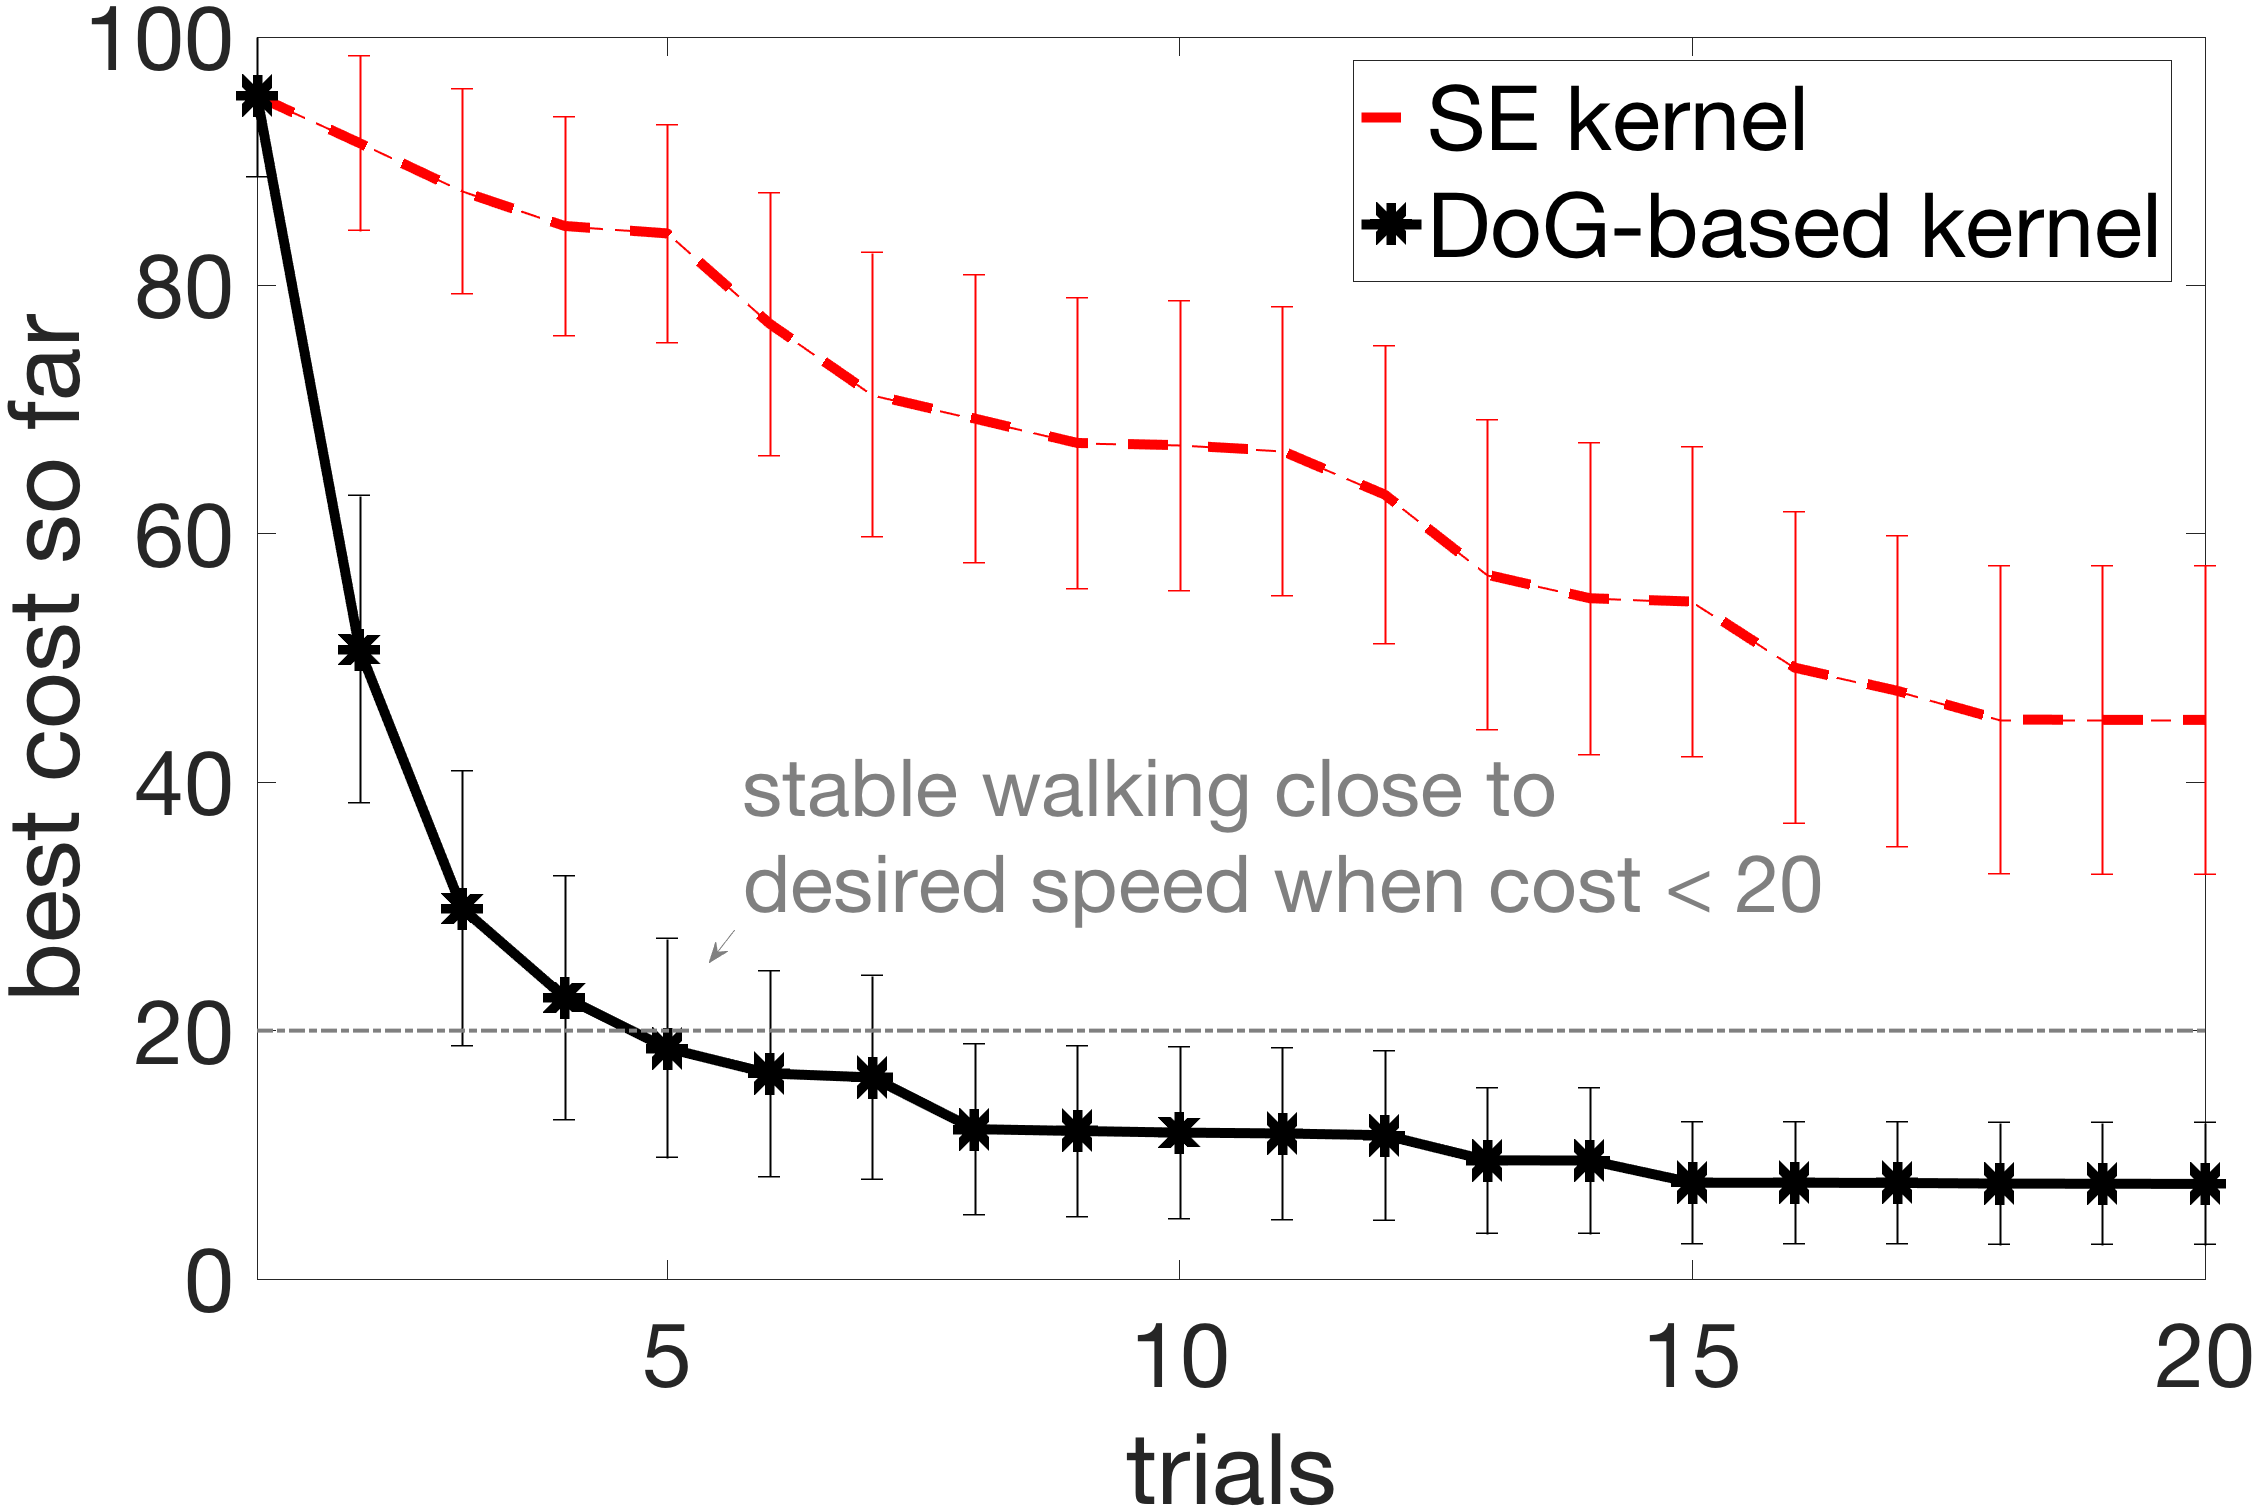
\includegraphics[width=0.6\textwidth]{img/sim_raibert_9d_speedupdown_disturbed_15.png}
\caption{\small{Further experiments using ATRIAS simulator: BO for ``speed-up-down'' target speed profile on robot model with mass and inertia differences
(mean over 50 runs; 95\% confidence intervals).}}
\label{fig:sim_9d_disturb}
\end{figure}

Figure~\ref{fig:sim_9d_disturb} illustrates BO on a simulated model with mass and inertia disturbances. The target was to start walking at 0.4m/s, then speed up to 0.6m/s, then 1.0m/s, slow down to 0.6m/s, then walk at 0.2m/s. \dogkernel was collected using an unperturbed model with a target speed of 0.5m/s, and yet it performed very well on this more challenging setting, with the top speed two times of the speed on which the kernel was collected. After 20 trials, 96\% of BO runs using the \dogkernel found a stable walking solution, compared to 56\% of the runs using an SE kernel. The average cost of the walking solutions was also improved: lower by $\approx$30\% when using DoG vs SE kernel.

These experiments suggest that \dogkernel is able to offer improvement for the settings different from the one used to generate it. This improvement is robust to both the deviations of the robot model/hardware parameters as well as desired walking speed profiles.

\subsection{Simulation experiments with the 50-dimensional controller}

\label{sec:vnmc_expt}
Next set of experiments were using the VNMC 50-dimensional controller, as described in Section \ref{sec:VNMC_cont} on the ATRIAS simulation.

VNMC does not start from rest, and needs an initial velocity. In previous work this has been emulated by either giving simulations initial speeds, or by giving a push. These are either un-realizable or unreliable on hardware. To overcome this problem, we start the VNMC with a \mbox{5-dimensional} walking controller (described in Section \ref{sec:raibert_cont}, parameters hand-tuned and fixed). Once the robot has taken 10 steps with this controller, the control is switched to VNMC. 

To construct \dogkernel for this controller we collected 250,000 points from 7-second simulations. The DoG scores were computed after switching to the VNMC (so after first 10 steps). Searching in 50 dimensional space could be completely intractable if the search region is too large. Usually enough domain knowledge is available to confine the search to a reasonably manageable region. We tried to hand-tune an initial point that walked 3-4 steps before falling in simulation (this point still had a very high cost of $\approx\!\!93$). This point became the ``center" of our search space, and we searched in a hyper-cube of size $[0.75, 1.25]$ in each dimension around this point. So, with initial point $x_0$, the search space was $[0.75 \cdot x_0 , 1.25 \cdot x_0]$. With these boundaries, 4\% of points sampled randomly in simulation were walking.

\begin{figure}[t]
\centering
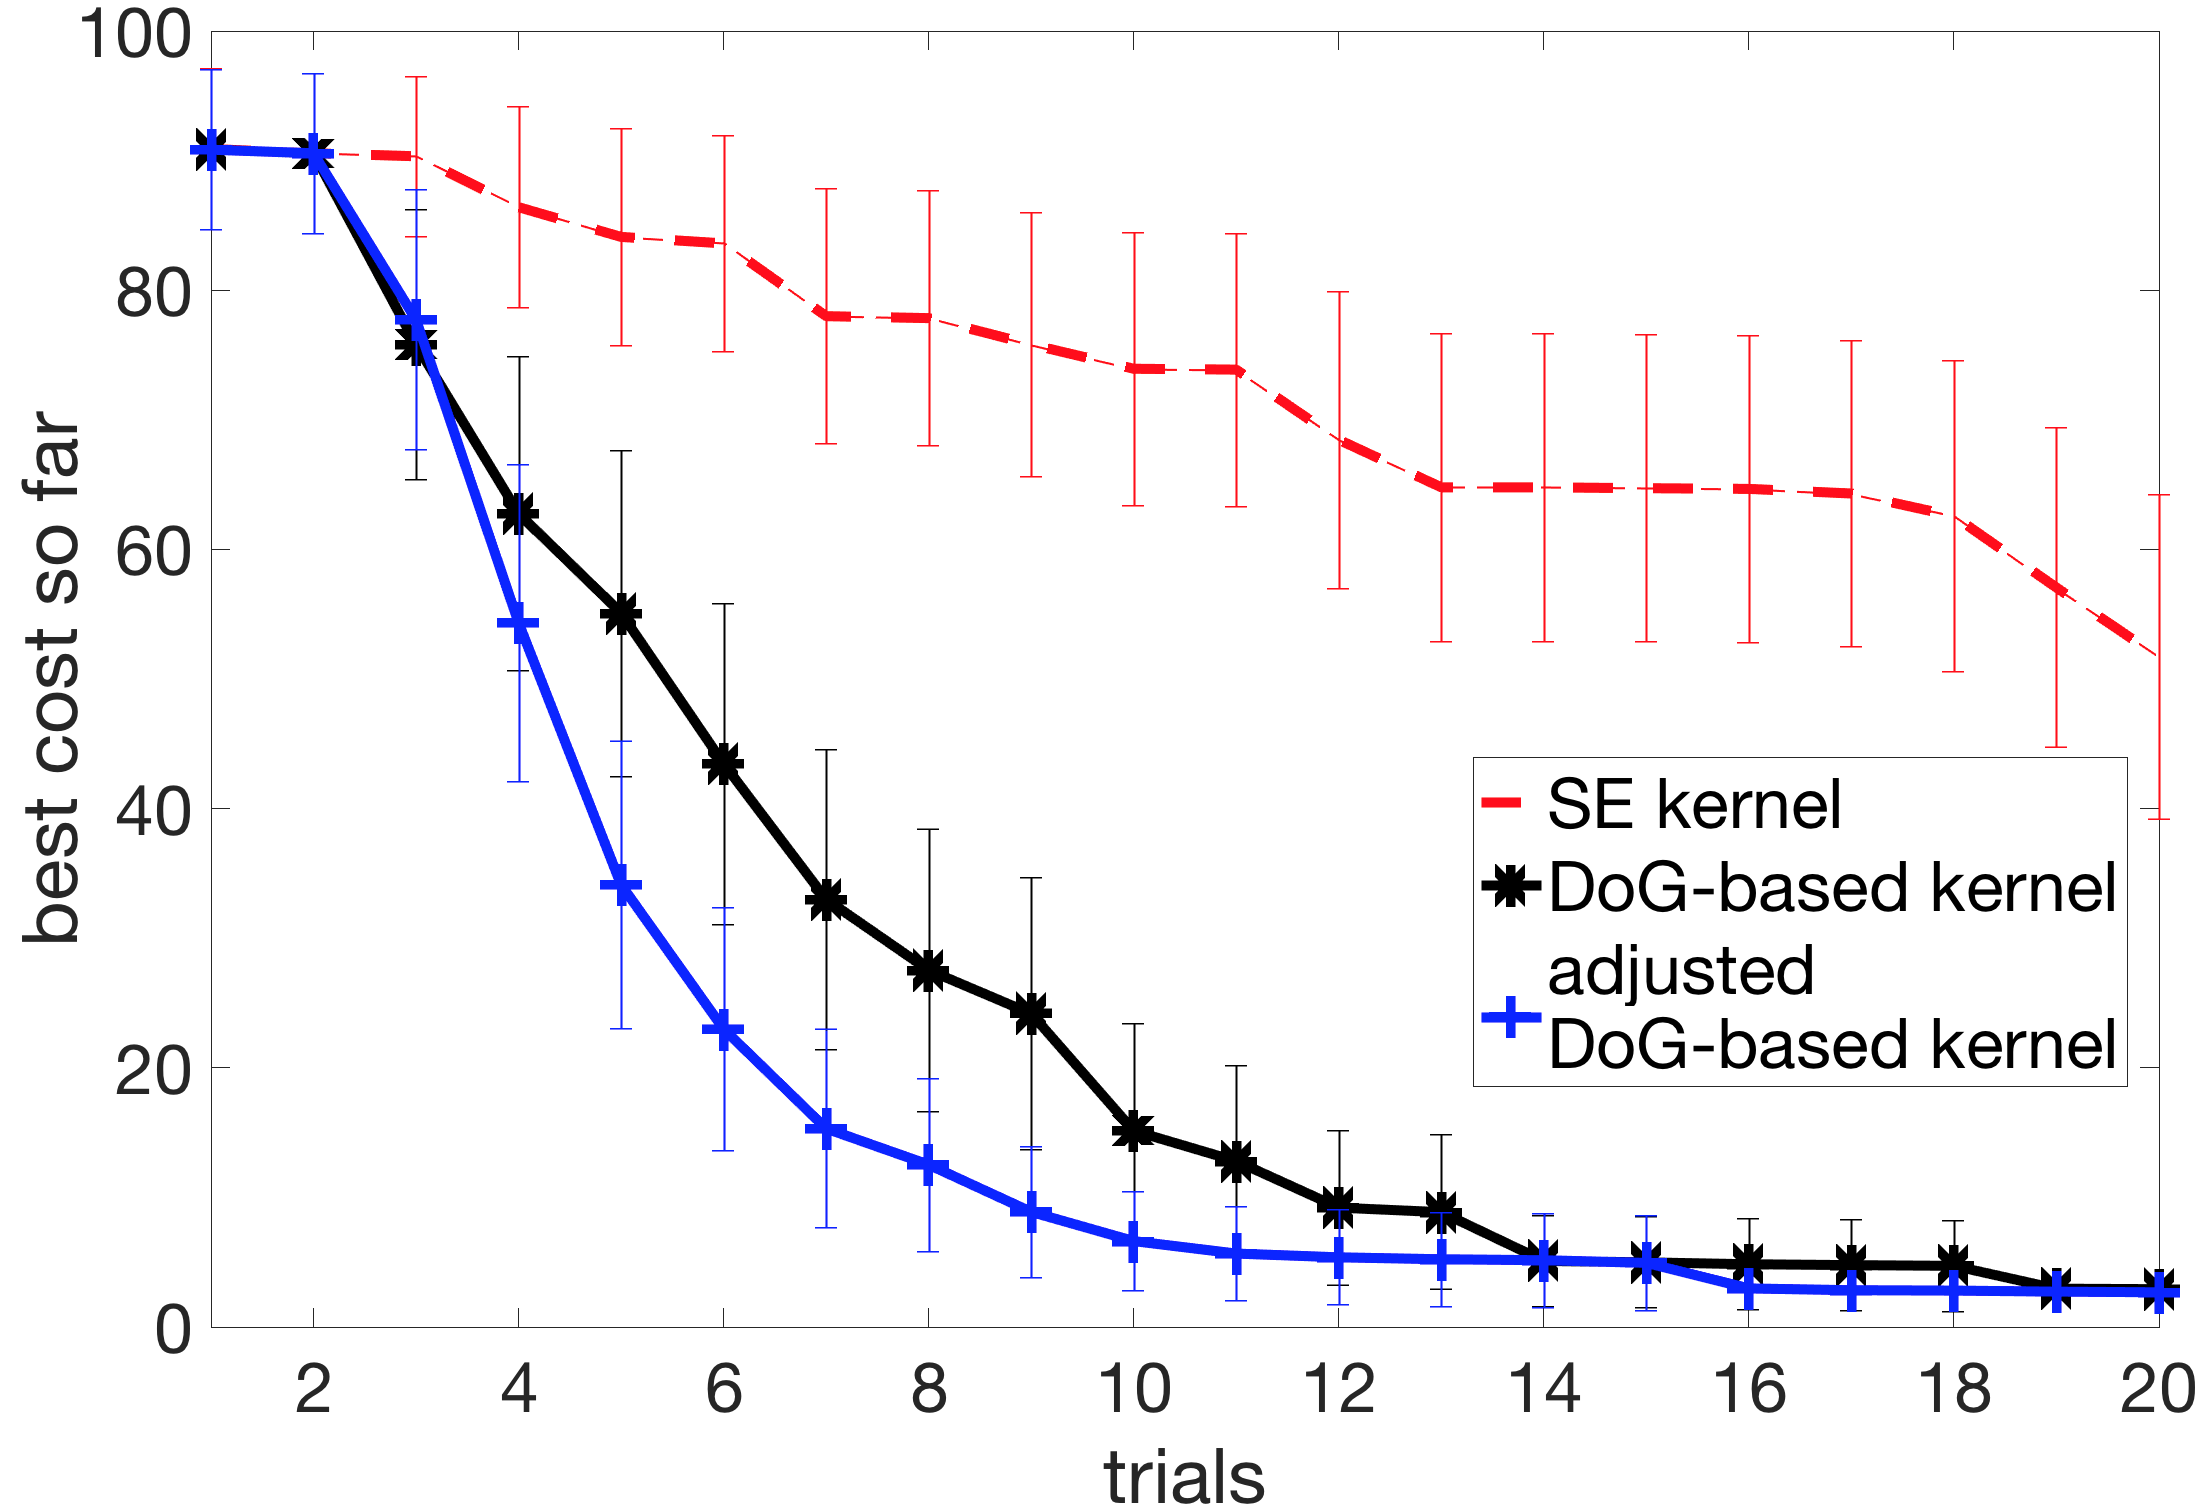
\includegraphics[width=0.6\textwidth]{img/sim_NM_Atrias_50d.png}
\caption{\small{BO with 50-dimensional Virtual Neuromuscular Controller on the ATRIAS simulation.}}
\label{fig:sim_NM_Atrias_50d}
\end{figure}

Figure \ref{fig:sim_NM_Atrias_50d} shows results of Bayesian Optimization with SE, \dogkernel and adjusted \dogkernel with mismatch information. During optimization simulations were run for $30$ seconds. We used the same cost function as described in the previous section (equation~\ref{eq:cost_sim}).

In 50-dimensional control, the mismatch between long and short simulations becomes apparent. This raises concerns for how useful \dogkernel would be on hardware, since it tries to infer the quality of the controller parameters from short simulations. 
For the 5-dimensional and 9-dimensional controllers, the performance during short simulations usually predicted whether $30s$ simulations would be successful. That is, points that walk for 5s would usually walk for 30s. However, this is not true for the 50-dimensional controller. Since this controller is capable of much richer behaviors, if a point is not in a limit cycle before the end of a short simulation, it can lead to a range of behaviours later. As a result, we noticed an improvement when using adjusted \dogkernel described in Section~\ref{sec:mismatch}. While DoG is still very competitive and finds walking points in 100\% of the runs by 20 trials, the adjusted DoG with mismatch has an advantage. It reaches the same performance as \dogkernel, but faster. 

%The 50-dimensional controller has not been fully implemented to work on hardware yet due to lack of time. However, our experiments on other controllers so far seem promising and we are working towards a hardware implementation. 
%\RA{describe current progress and interest in this controller being ultimately used on hw ~\ref{van2015experimental}}
To anticipate potential mismatch between simulation and hardware, we tested it on slightly perturbed initial conditions for the VNMC. The different conditions were aimed to replicate issues likely to be seen on hardware. The starting states for VNMC would differ slightly each time, since they would depend on the state of the robot after the 5-dimensional initiating controller has finished. Both DoG and adjusted DoG were robust to slight changes in initial condition. 

It would be interesting to study the effect of a mismatch map on performance on hardware. While essentially a mismatch map adds more parameters to learn, which would result in a slower optimization, if initialized properly with domain knowledge, it might help. The \dogkernel samples a few unstable points in the start of the 50-dimensional optimization, as these have high DoG scores on short simulations, but still might fall in longer simulations under disturbances. Since a lot of the 50-dimensional space is clustered around each DoG score, its an over-condensation of the space. A lot of potentially good points get rejected because one of the points falls. If we detect a mismatch at the high DoG point that fell, and effectively increase its distance to other high DoG points, we will help speed up the optimization.

%We plan to test adjusted \dogkernel more in the future in this challenging setting that could be sensitive to simulation-hardware mismatch. 

\subsection{Simulation experiments on a 16-dimensional controller}
\label{sec:probform}
To make sure that our feature transform generalizes to multiple robot morphologies, we also did experiments on the 7-link biped, described in Section \ref{sec:7_link_biped}.

\begin{figure}[t]
\centering
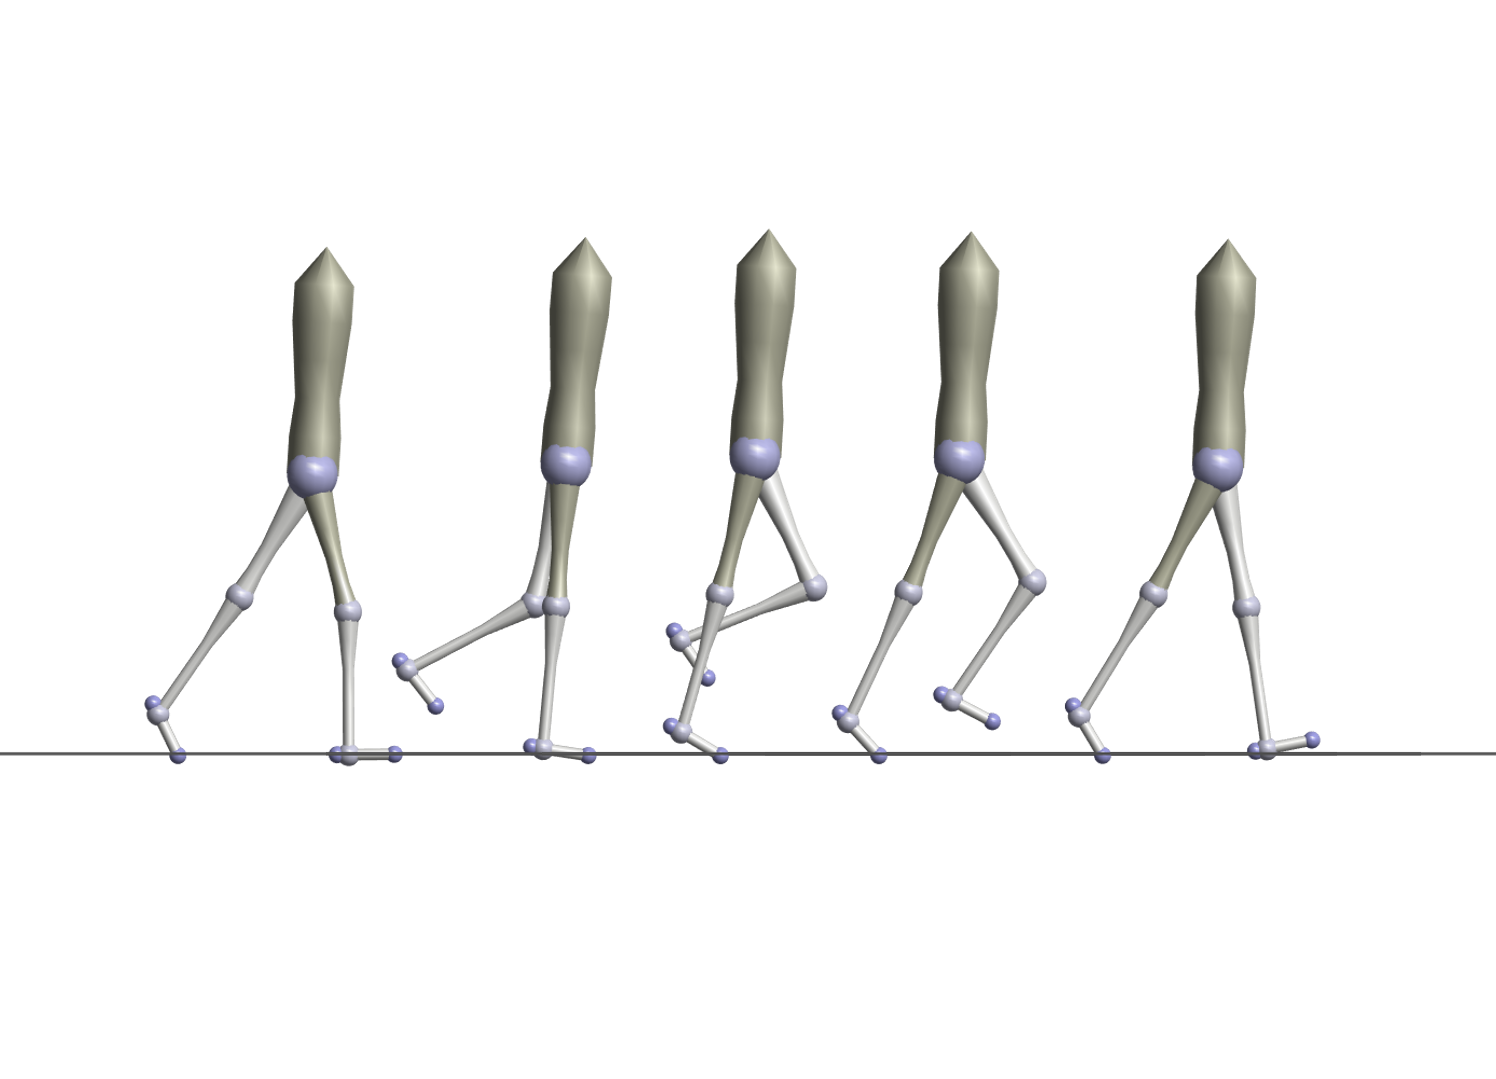
\includegraphics[width=0.35\textwidth]{img/walk_flat.png}
\hspace{10px}
\vspace{-40px}
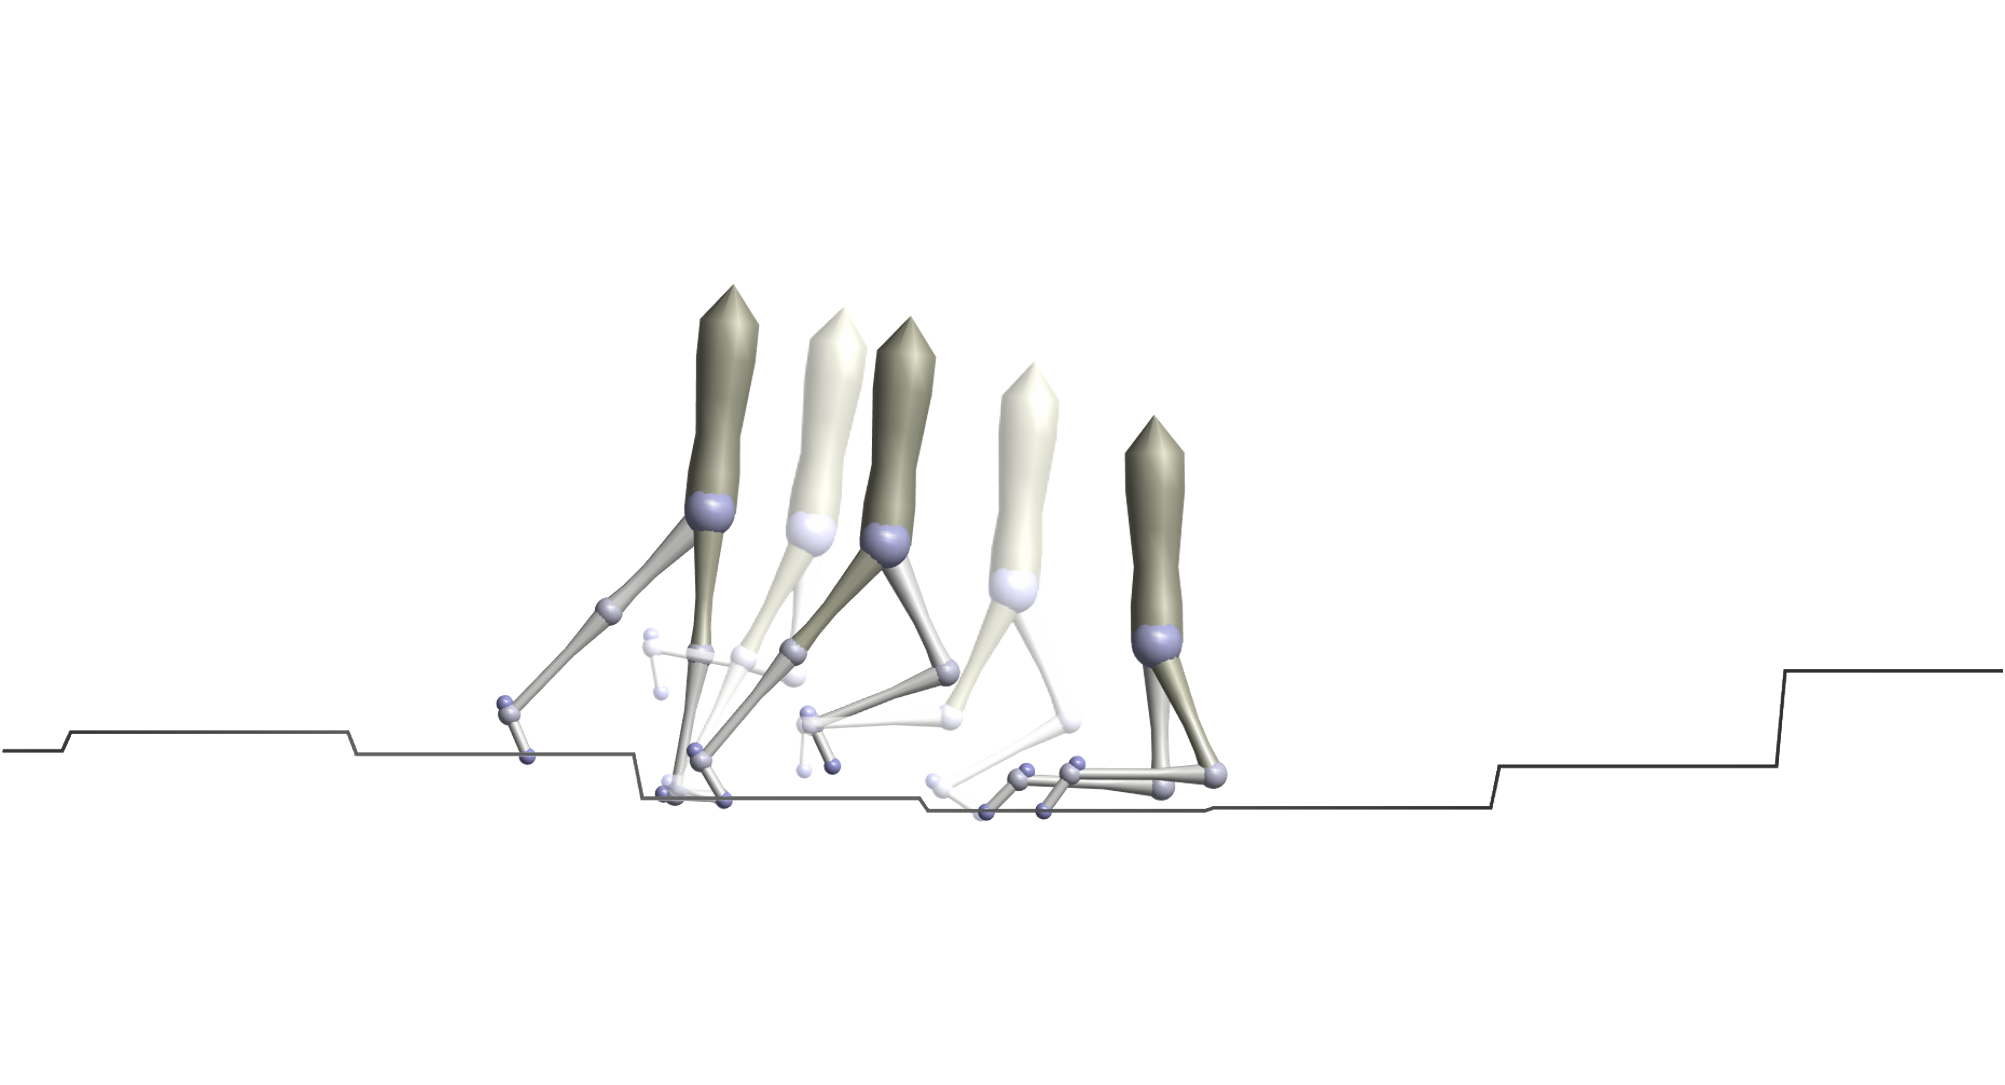
\includegraphics[width=0.5\textwidth]{img/rough_fall.png}
\label{fig_bo_locomotion_visualization_rough}
\vspace{30px}
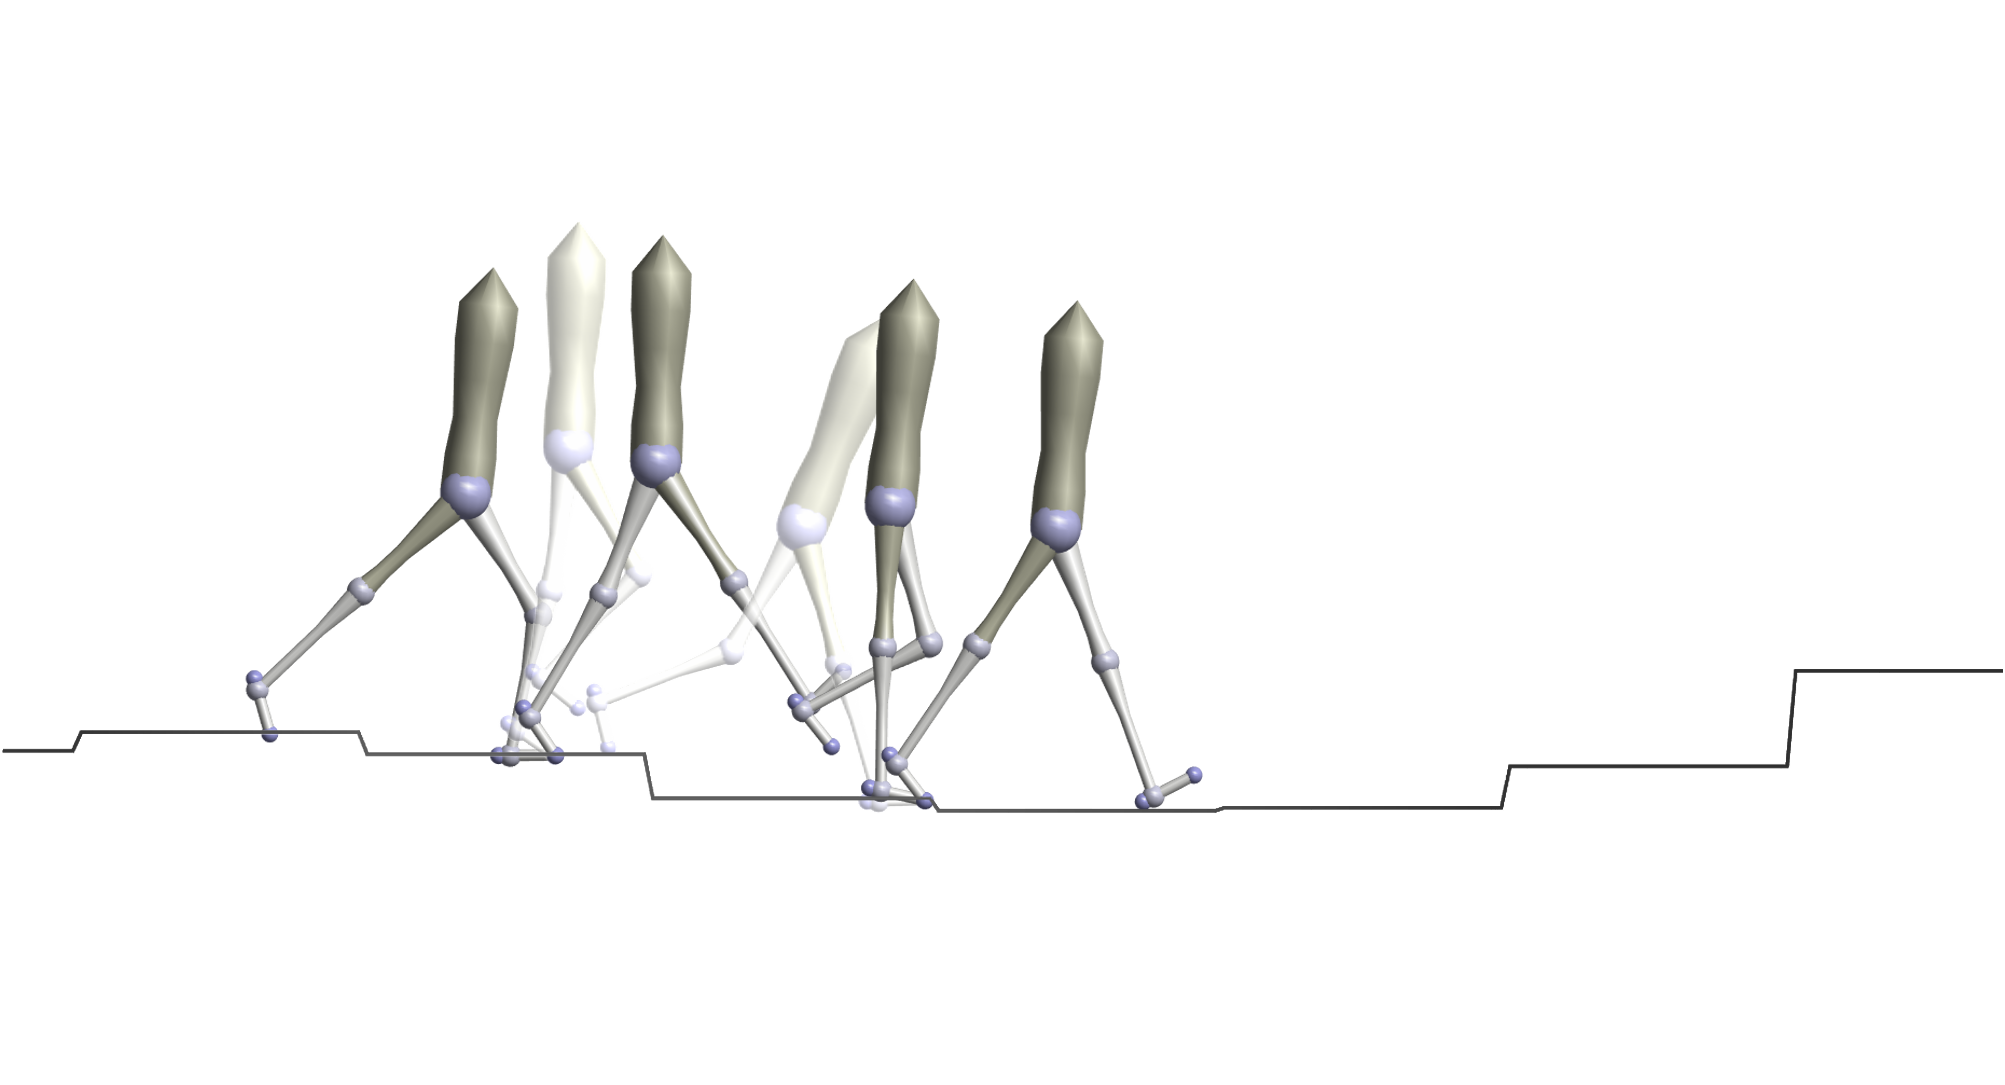
\includegraphics[width=0.5\textwidth]{img/rough_walk.png}
\caption{Top row: a policy that generates successful walking on flat ground could fail on rough ground. Bottom row: optimization on rough ground finds policies that walk, even though pre-computation for DoG kernel is done using unperturbed model on flat ground.}
\label{fig_bo_locomotion_visualization_flat}
\end{figure}

We conduct our experiments on models with mass and inertial disturbances and on different ground profiles. After collecting the DoG scores, we perturb the mass of each link, inertia and center of mass location randomly by up to $15\%$ of the original value. For mass/inertia we randomly pick a variable from a uniform distribution between $[-0.15,\ 0.15] \cdot M$, where $M$ is the original mass/inertia of the segment. Similarly we change the location of the center of mass by $[-0.15,\ 0.15] \cdot L/2$, where $L$ is the length of the link. These disturbances are different for each run of our algorithm, hence we test a wide range of possible modelling disturbances.
For the ground profiles, we generate random ground height disturbances of upto $\pm 8cm$ per step.

To ensure that our approach can perform well across various cost functions, we conduct experiments on two different costs, constructed such that parameter sets achieving low cost also achieve stable and robust walking gaits. The first cost function varies smoothly over the parameter space:
 
\begin{align}
cost = \frac{1}{1+t} + \frac{0.3}{1+d} + 0.01 (v-v_{tgt}),
\end{align}
where $t$ is seconds walked, $d$ is the final CoM position, $v$ is mean velocity and $v_{tgt}$ is the desired walking velocity (from human data). This cost encourages walking further and for longer through the first two terms, and penalizes deviating from the target velocity with the last.

The second cost function is a slightly modified version of the cost used in~\cite{song2015neural} for experiments with \mbox{CMA-ES}, also similar to the cost described in previous sections. It penalizes policies that lead to falls in a non-smooth manner:
\begin{align}
cost_{CMA} = 		
    \begin{cases}
		300 - x_{fall} , \text{\small{if fall}} \\
		100 ||v_{avg} - v_{tgt}|| + c_{tr}, \text{\small{if walk}}\\
	\end{cases}
\end{align}
Here $x_{fall}$ is the distance travelled before falling, $v_{avg}$ is the average speed in simulation, $v_{tgt}$ is the target speed and $c_{tr}$ is the cost of transport calculated using muscle activations. The first term directly penalizes policies that result in a fall, inversely to the distance walked. If the model walks for the whole simulation time, the cost is lower, ensured by the constants, and encourages policies that result in lower cost of transport and walk at target velocity. Since we have the same set of gains for left and right legs, the steadiness cost of the original cost~\cite{song2015neural} was unimportant. So, we removed that term and focused on the first and second conditions in the optimization.

In the following sections we compare the performance of several baseline and state-of-the-art optimization algorithms in simulation. Motivated by the discussion in~\cite{calandra2016bayesian}, we include the baseline of uniform random search. While this search is uninformed and not sample-efficient, it could (perhaps surprisingly) serve as a competitive baseline in non-convex high-dimensional optimization problems. 
%Theoretically -- it provides statistical guarantees of convergence, and practically -- it can outperform informed algorithms as well as grid search on high-dimensional problems (see Section~2~in~\cite{calandra2016bayesian} for further discussion).

We also provide comparisons with \mbox{CMA-ES}~\cite{hansen2006cma} and Bayesian Optimization with a Squared Exponential kernel (basic BO). Since we were optimizing a non-convex function in a 16D space, it was not feasible to calculate the global minimum exactly. To estimate the global minimum for the costs we used, we ran CMA-ES (until convergence) and BO with our domain kernel (for 100 trials) for 50 runs without model disturbances on flat ground. 
When reporting results, we plot the best results found in this easier setting as the estimated optimum for comparison.

All the experiments described below are done for 50 independent runs, each with a unique set of modeling disturbances and a different ground profile for rough ground walking. Each run  consists of 100 trials or cost function evaluations, in which the optimization algorithm evaluates a parameter set for 100 seconds of simulation. Note that the disturbances and ground profiles remain constant across each run (100 trials).

\subsubsection{Experiments on the smooth cost function}

\begin{figure}[t]
\centering
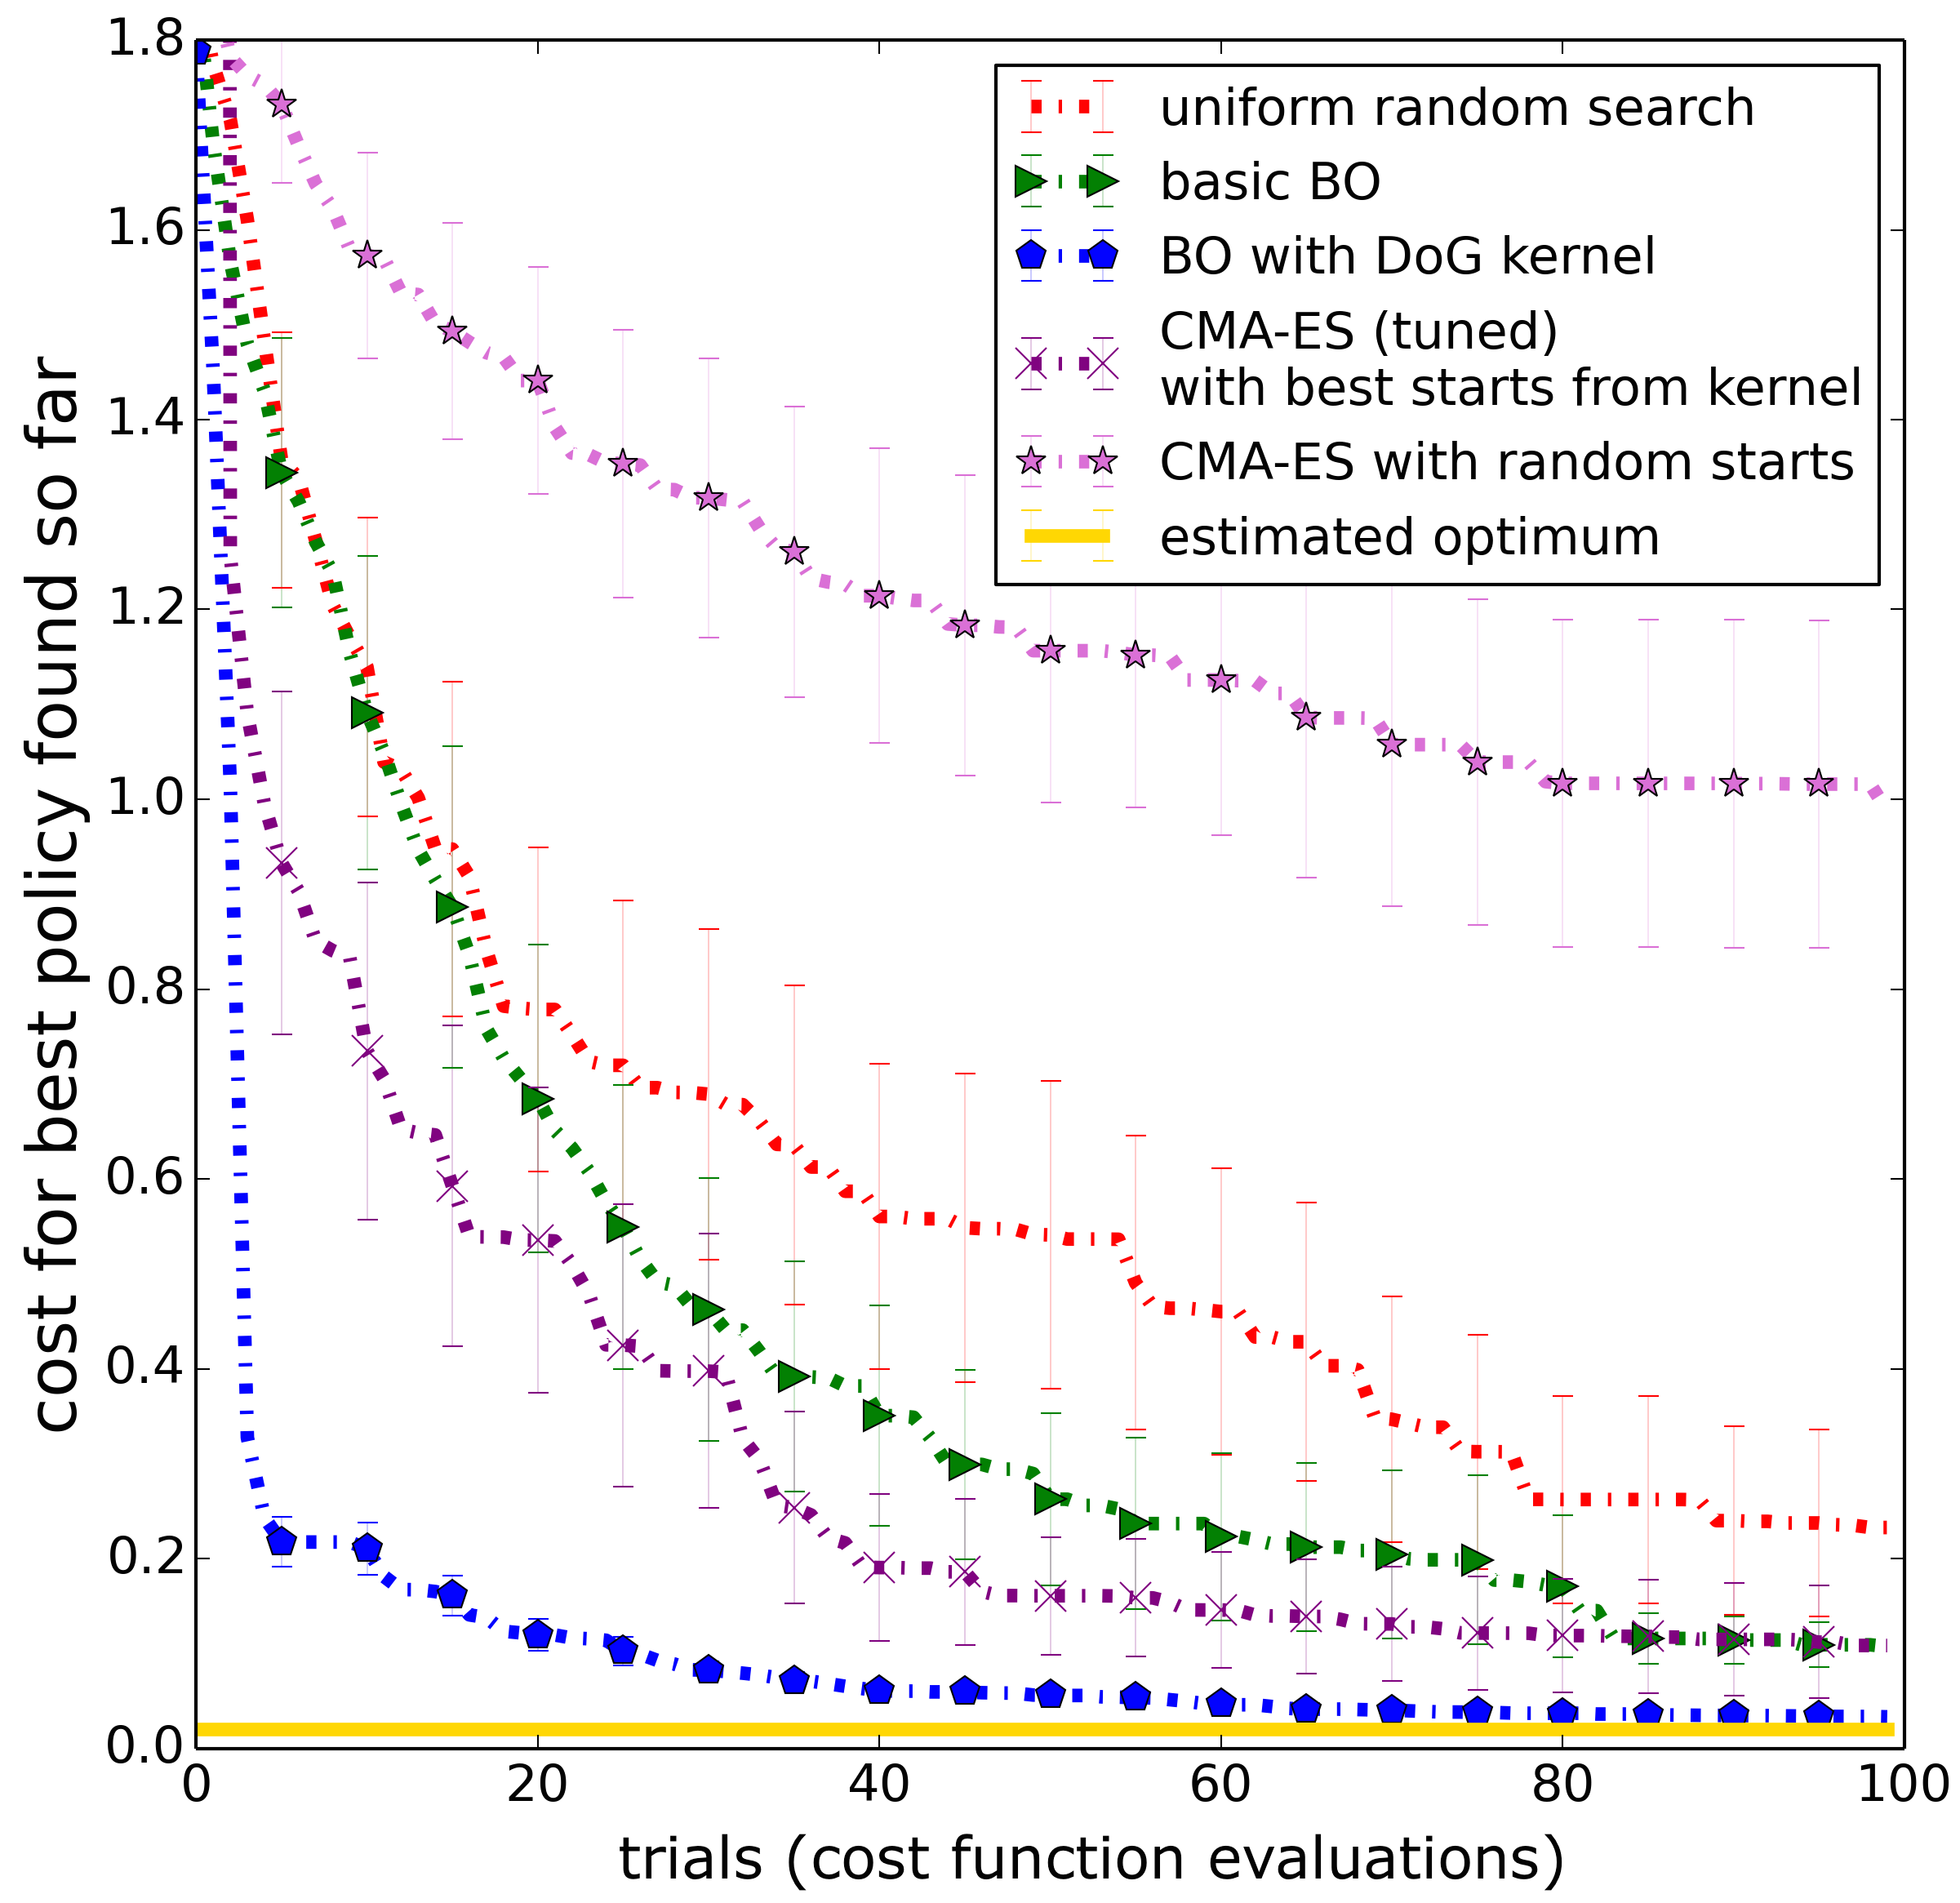
\includegraphics[width=0.6\textwidth]{img/rnd_bo_bo_covLoc_cma_rough6_disturb_smooth_cost.png}
\caption{Experiments using DoG kernel on rough ground with model disturbances on the smooth cost over 50 runs. Basic BO line (green triangles) was obtained using BO with a Euclidean distance kernel. Estimated optimum (yellow line) was obtained on the unperturbed setting. BO with \dogkernel kernel (blue pentagons) used the DoG feature transform and was substantially more sample-efficient than the alternative approaches.}
\label{fig_bo_locomotion}
\end{figure}

Figure~\ref{fig_bo_locomotion} shows results of our experiments using the \dogkernel kernel on the smooth cost.
Policies with costs of less than $\approx\!\!0.15$ corresponded to robot model walking on rough ground with $\pm 8 cm$ disturbance.
For BO with \dogkernel kernel, 25-30 cost function evaluations were sufficient to find points that corresponded to robot model walking on a randomly generated rough ground. This is in contrast to basic BO that did not find such results in under 100 trials. 

To let CMA-ES also benefit from the kernel, we started each run from one of the best 100 points for the \dogkernel kernel. After tuning the $\sigma$ parameter of CMA-ES to make it exploit more around the starting point, we were able to find policies that resulted in walking on rough ground after 65-70 cost function evaluations on most runs. On the other hand, \mbox{CMA-ES} starting from a random initial point was not able to find walking policies in 100 evaluations.

These results suggest that DoG scores successfully captured useful information about the parameter space and were able to effectively focus BO and CMA-ES on the promising regions of the policy search space. 

\subsubsection{Experiments with the non-smooth cost}

\begin{figure}[t]
\centering
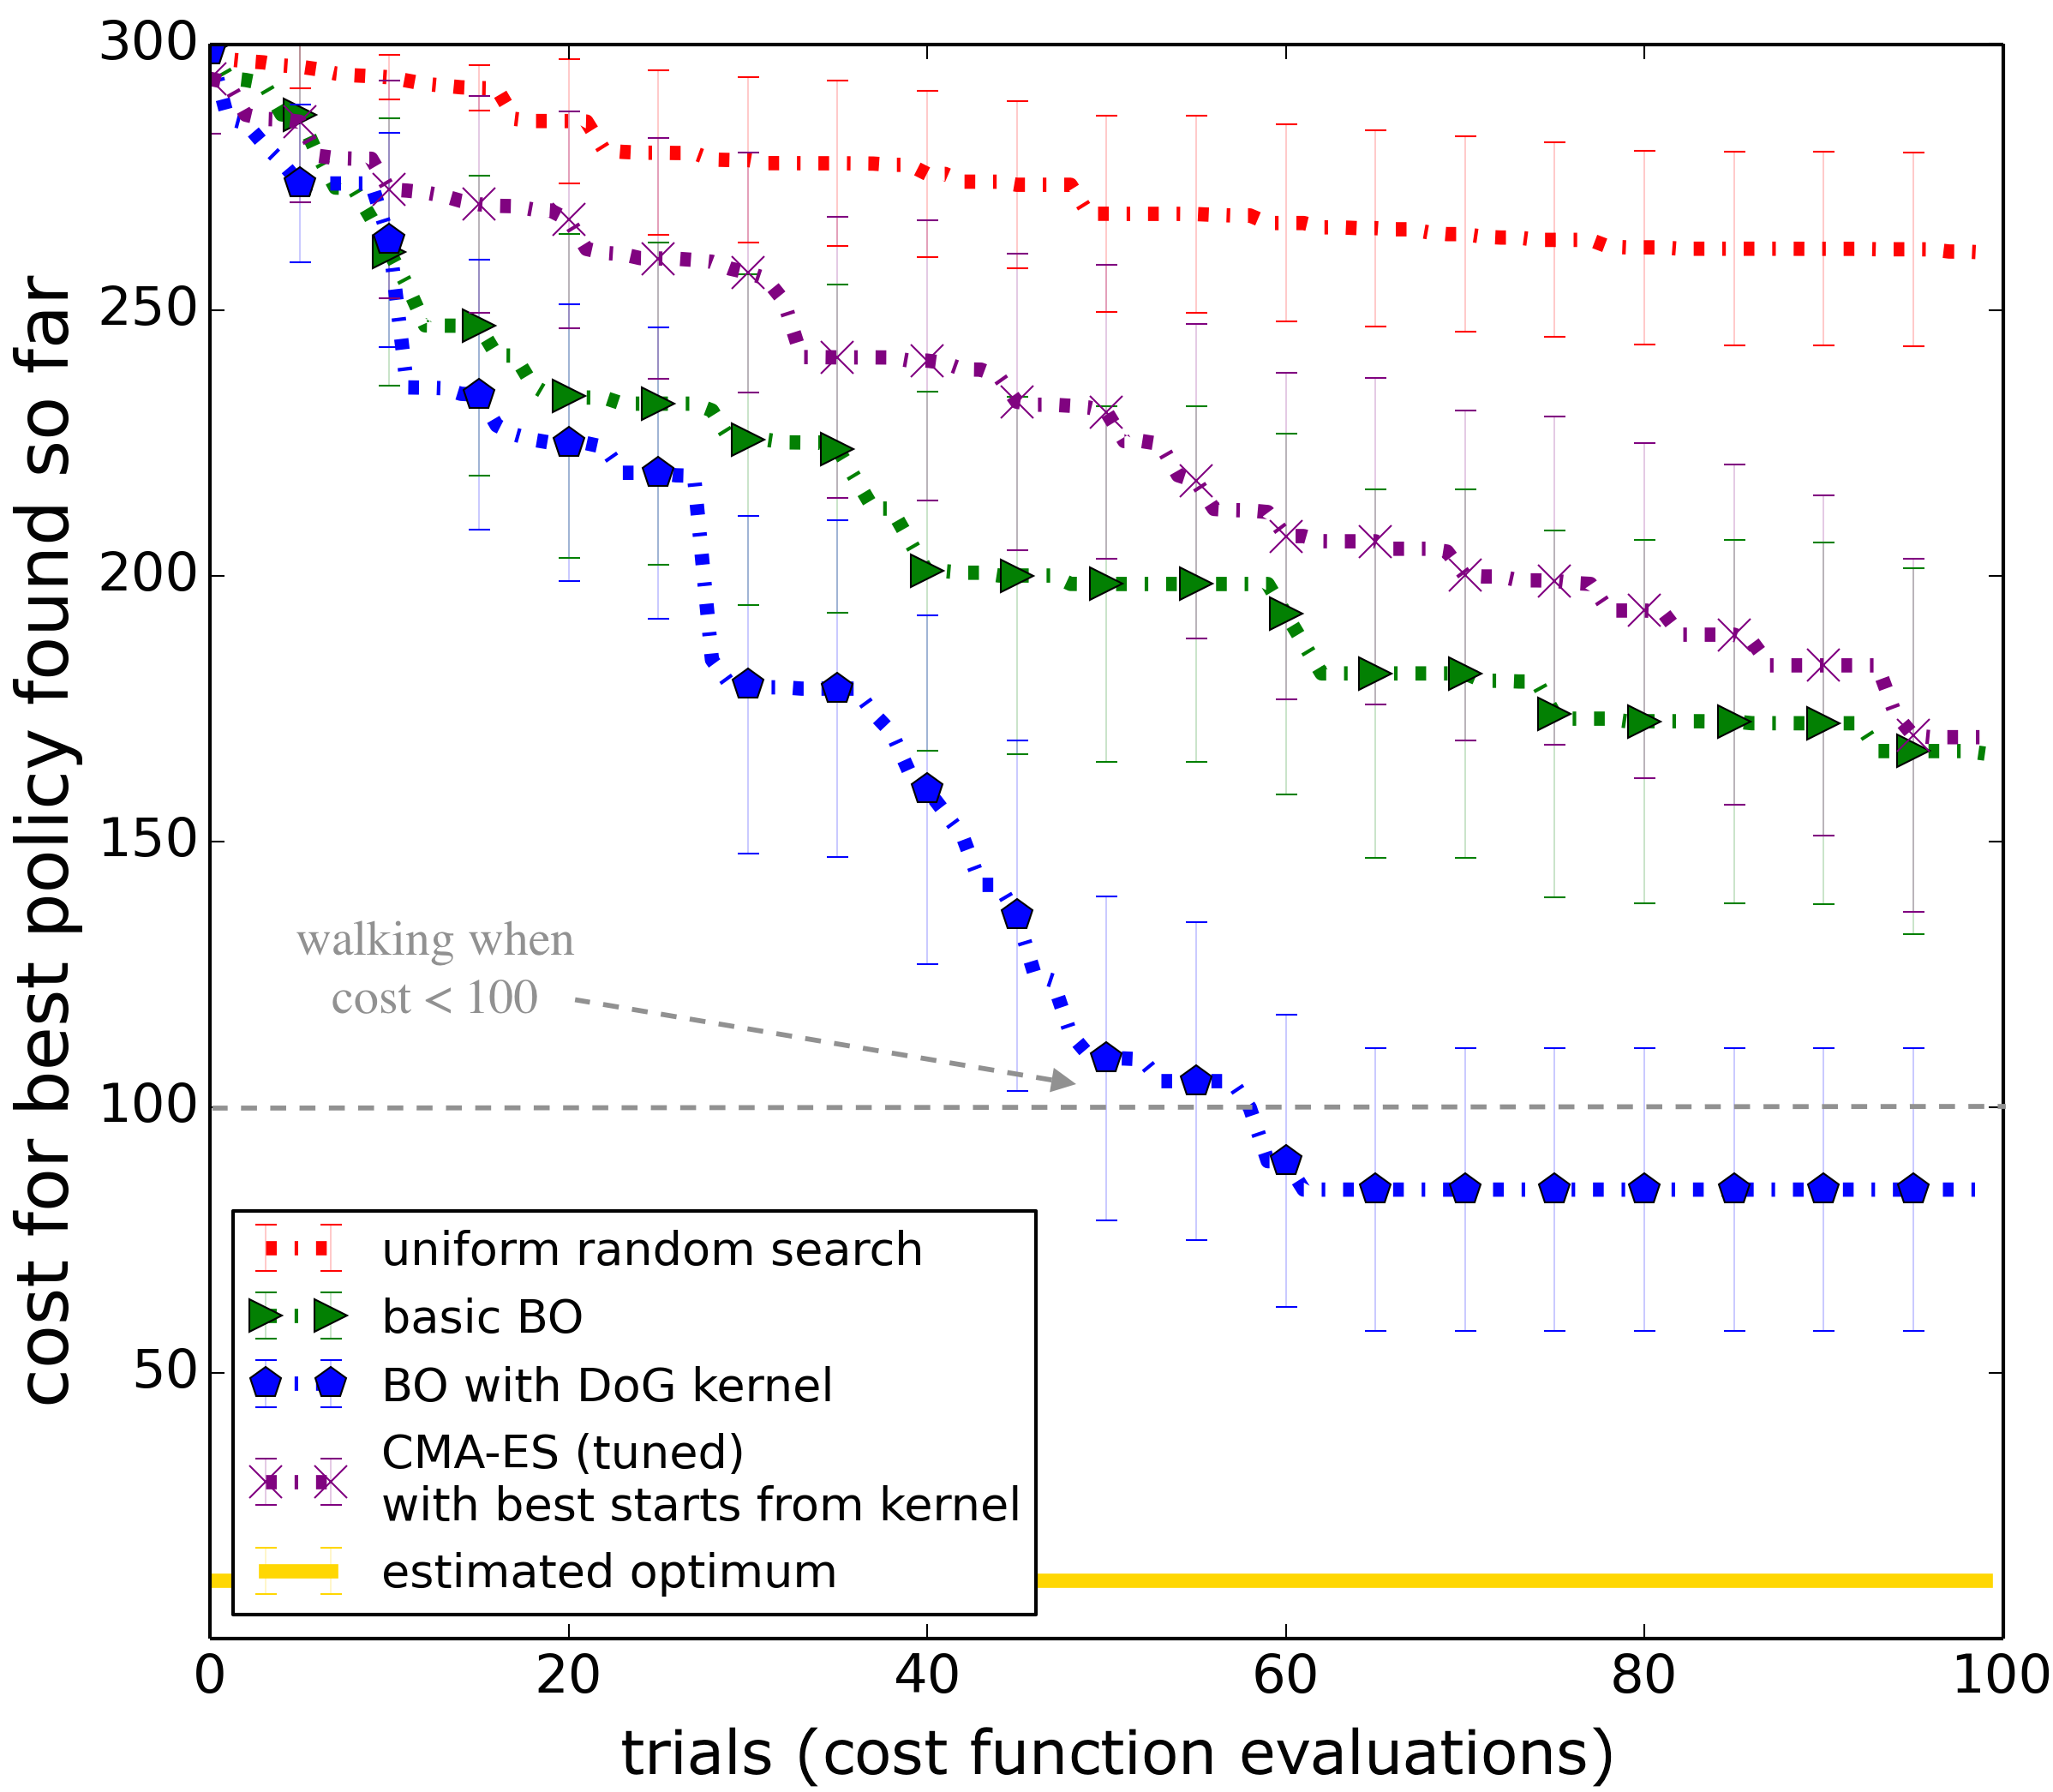
\includegraphics[width=0.6\textwidth]{img/rnd_bo_bo_covLoc_cma_rough6_disturb_nonsmooth_cost.png}
\caption{Experiments using \dogkernel kernel on rough ground with model disturbances on the non-smooth cost over 50 runs. Policies with costs below 100 generate walking behaviour for 100 seconds in simulation. None of the optimization methods find optimal policies in all the runs and hence the mean cost is higher than the estimated optimum.}
\label{fig_bo_locomotion_non_smooth}
\end{figure}

We observed good performance on the non-smooth cost function (Figure \ref{fig_bo_locomotion_non_smooth}), though it was not as remarkable as the smooth cost. BO with kernel still outperformed all other methods by a margin, but this different cost seems to hurt BO and \mbox{CMA-ES} alike. Since this cost is discontinuous, there is a huge discrepancy between costs for parameters that walk and those that don't. If no walking policies are sampled, BO learns little about the domain and samples randomly, which makes it difficult to find good parameters. Hence not all runs find a walking solution. BO was able to find successful walking in $74\%$ of cases on rough ground with $\pm 6 cm$ disturbance in less than 60 trials/evaluations. \mbox{CMA-ES} starting from a good kernel point was able to do it in $40\%$ of runs. 

This showed that our kernel was indeed independent of the cost function to an extent, and worked well on two very different costs. We believe that the slightly worse performance on the second cost is because of the cost structure, rather than a kernel limitation, as it still finds walking solutions for a significant portion of runs.  


\subsubsection{Experiments on different terrains}

\begin{figure}[t]
\centering
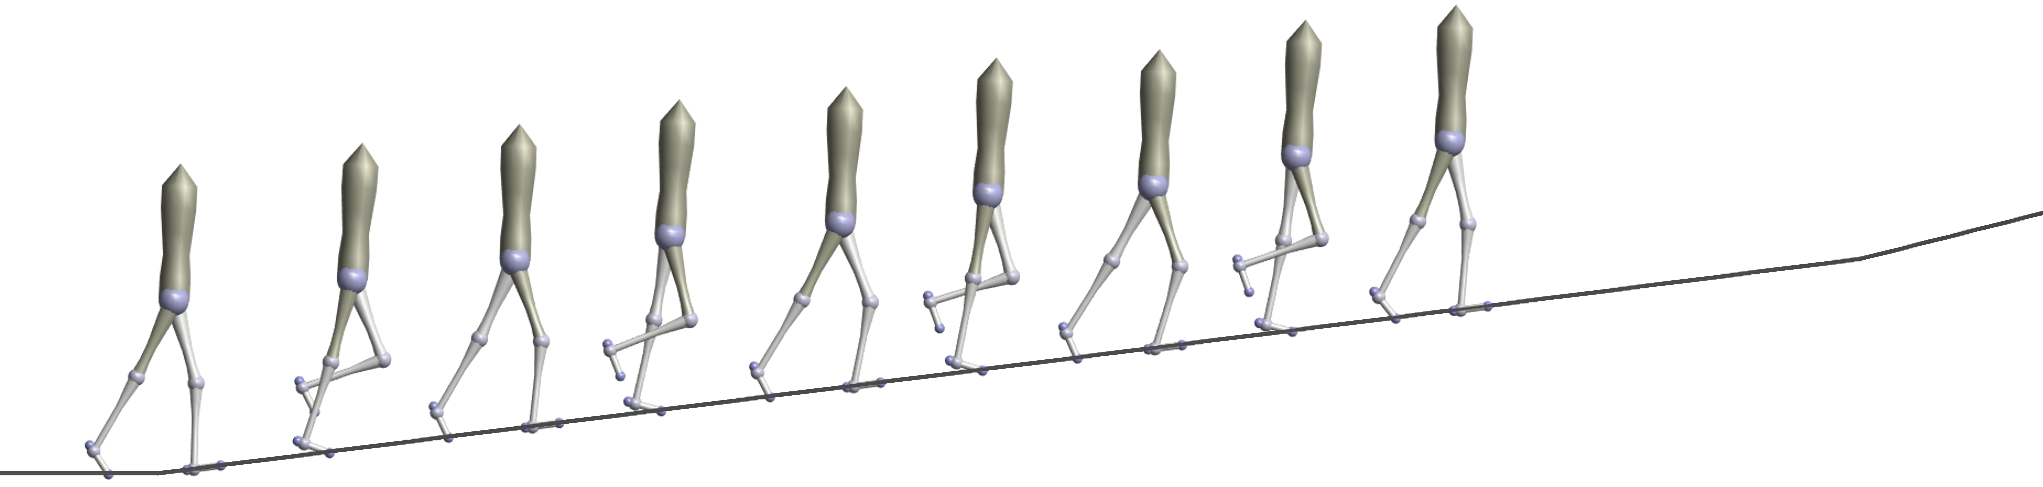
\includegraphics[width=0.8\textwidth]{img/rampup.png}
\vspace{10px}
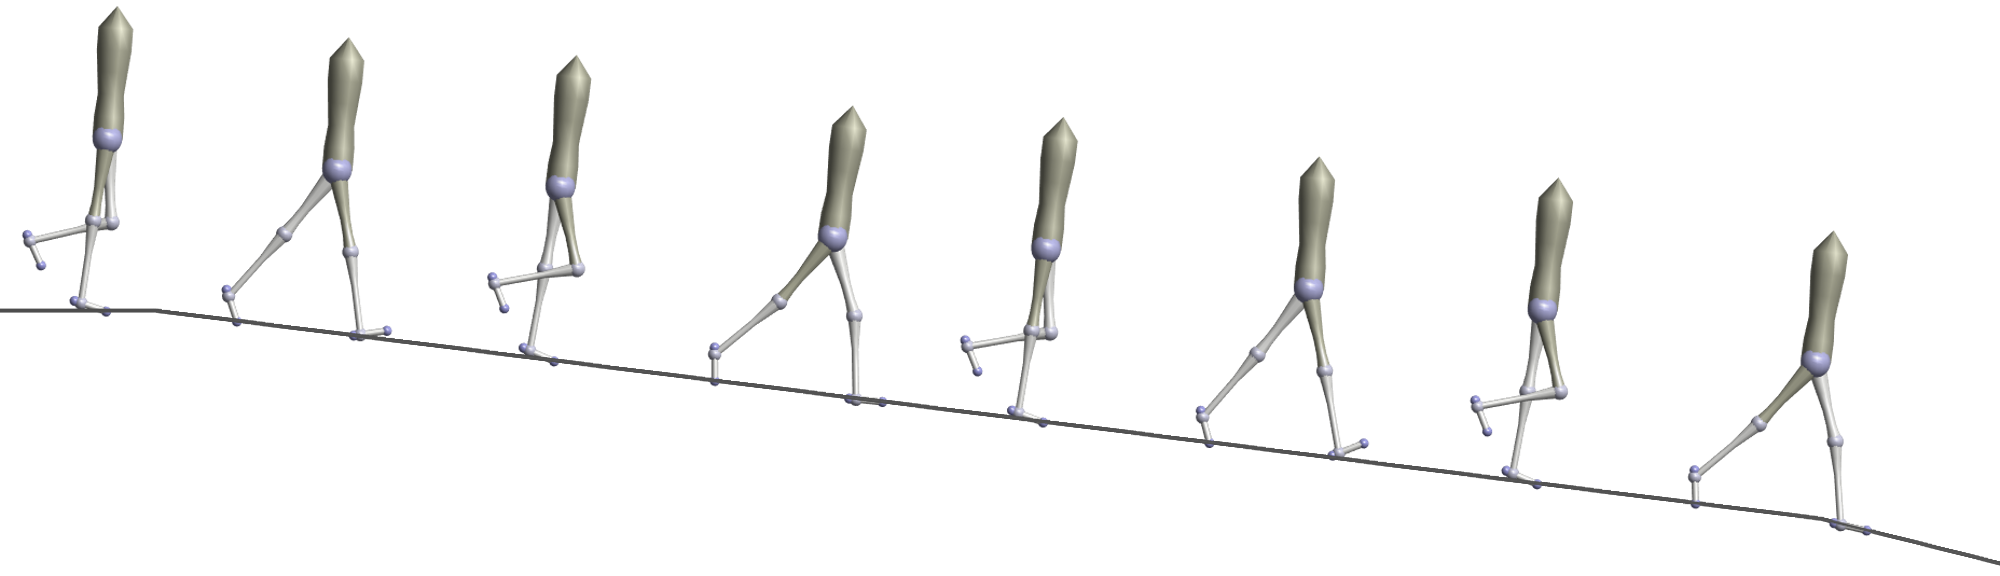
\includegraphics[width=0.8\textwidth]{img/rampdown.png}
\caption{Optimized policies walking up and down a $12.5 \%$ ramp.}
\label{fig_ramp}
\end{figure}

We also optimized on ramps -- sloping upwards, as well as downwards, with the kernel generated on flat ground. The ramp up and down ground slopes were gradually increased every $20m$, until the maximum slope was reached. The maximum slopes for going down and going up were $20\%$ ($tan(\theta) = 0.2, \theta=11.31\deg$). BO with DoG kernel was able to find parameters that walked for 100 seconds in $50\%$ of cases in ramp up and $90\%$ in ramp down. Example optimized policies walking up and down slope are shown in Figure \ref{fig_ramp}.

We believe the reason we could not find walking policies on ramps in all runs, was that we are not optimizing the hip lean, which was noted to be crucial for this profile in \cite{song2015neural}. Since we did not consider this variable when generating our 16 dimensional kernel, it was not trivial to optimize over it without re-generating the grid. Similarly, we found that we could not find any policies that climbed up stairs. Perhaps this could be achieved when optimizing over a much larger set of parameters, as in \cite{song2015neural}. 

To test if the hip lean indeed helps climb up a ramp, we hand-tuned the hip lean to be $15^{\deg}$, instead of the original angle of $6^{\deg}$ for which the kernel was generated. Indeed, our rate of success on walking on ramp up ground profile increased from $50\%$ to $65\%$. %For walking upstairs, we achieved $10\%$ success. 
This shows that the hip lean indeed helped walking on these terrains, and ideally we would like to optimize it along with the other parameters. Also, it shows that the \dogkernel kernel is robust to changes in parameters that were used to generate it. This is an important property, as parameters in the neuromuscular model are changed slightly for different experiments, for example the ground stiffness, initial conditions of the model, etc. If the kernel results hold across a variety of such conditions, we don't need to regenerate it.

%In the future, we would like to include more variables for optimizing over different terrains, and include them as part of the kernel. 

\subsection{Summary of experiments with the DoG transform}

\AR{Add a table summarizing results from previous section}

\section{Experiments with the NN transform}

In this section we describe our experiments with cost-based and trajectory-based neural network kernels, described in Section \ref{}. We first consider the setting of optimizing a 5-dimensional controller for the ATRIAS robot from Section \ref{sec:raibert_cont}. We show that the cost-based kernel is able to improve sample efficiency over standard Bayesian Optimization. We present hardware experiments to demonstrate that our kernel allows obtaining a set of parameters close to optimal on the second trial for a constant target speed. With a variable target speed, it can find walking controllers reliably in 5 trials.

Next, we discuss simulation experiments with a 16 dimensional controller that utilizes a Neuromuscular model from Section \ref{} on a 7-link biped. These experiments show that our trajectory-based kernel is able to significantly outperform standard Bayesian optimization for a higher-dimensional controller even when a sharply discontinuous cost is used during optimization.

\subsection{Hardware experiments with a 5-dimensional controller}
\label{experiments_atrias}

For our experiments on the ATRIAS robot we used a high-fidelity ATRIAS simulator from ~\cite{martin2015robust} to generate the data for learning the network. 
%We did an initial analysis of the performance of our approach in simulation, followed by hardware experiments. 
%Then we conducted a set of hardware experiments on the ATRIAS robot using a controller described in Section~\ref{sec:probform}. 
We constructed a distance metric for a kernel used in Bayesian Optimization by training a neural network to reconstruct cost obtained from short simulations. We created a sobol grid on the input parameter space with 20000 points and ran short 3.5 second simulations on each of the corresponding 20000 parameter sets to compute the costs. We then used a fully connected network with 4 hidden layers (128, 64, 16, 4 units) with L1 loss to reconstruct the transformation of the cost described in section~\ref{sec:approach_asym}.

%\begin{figure}
%\centering
%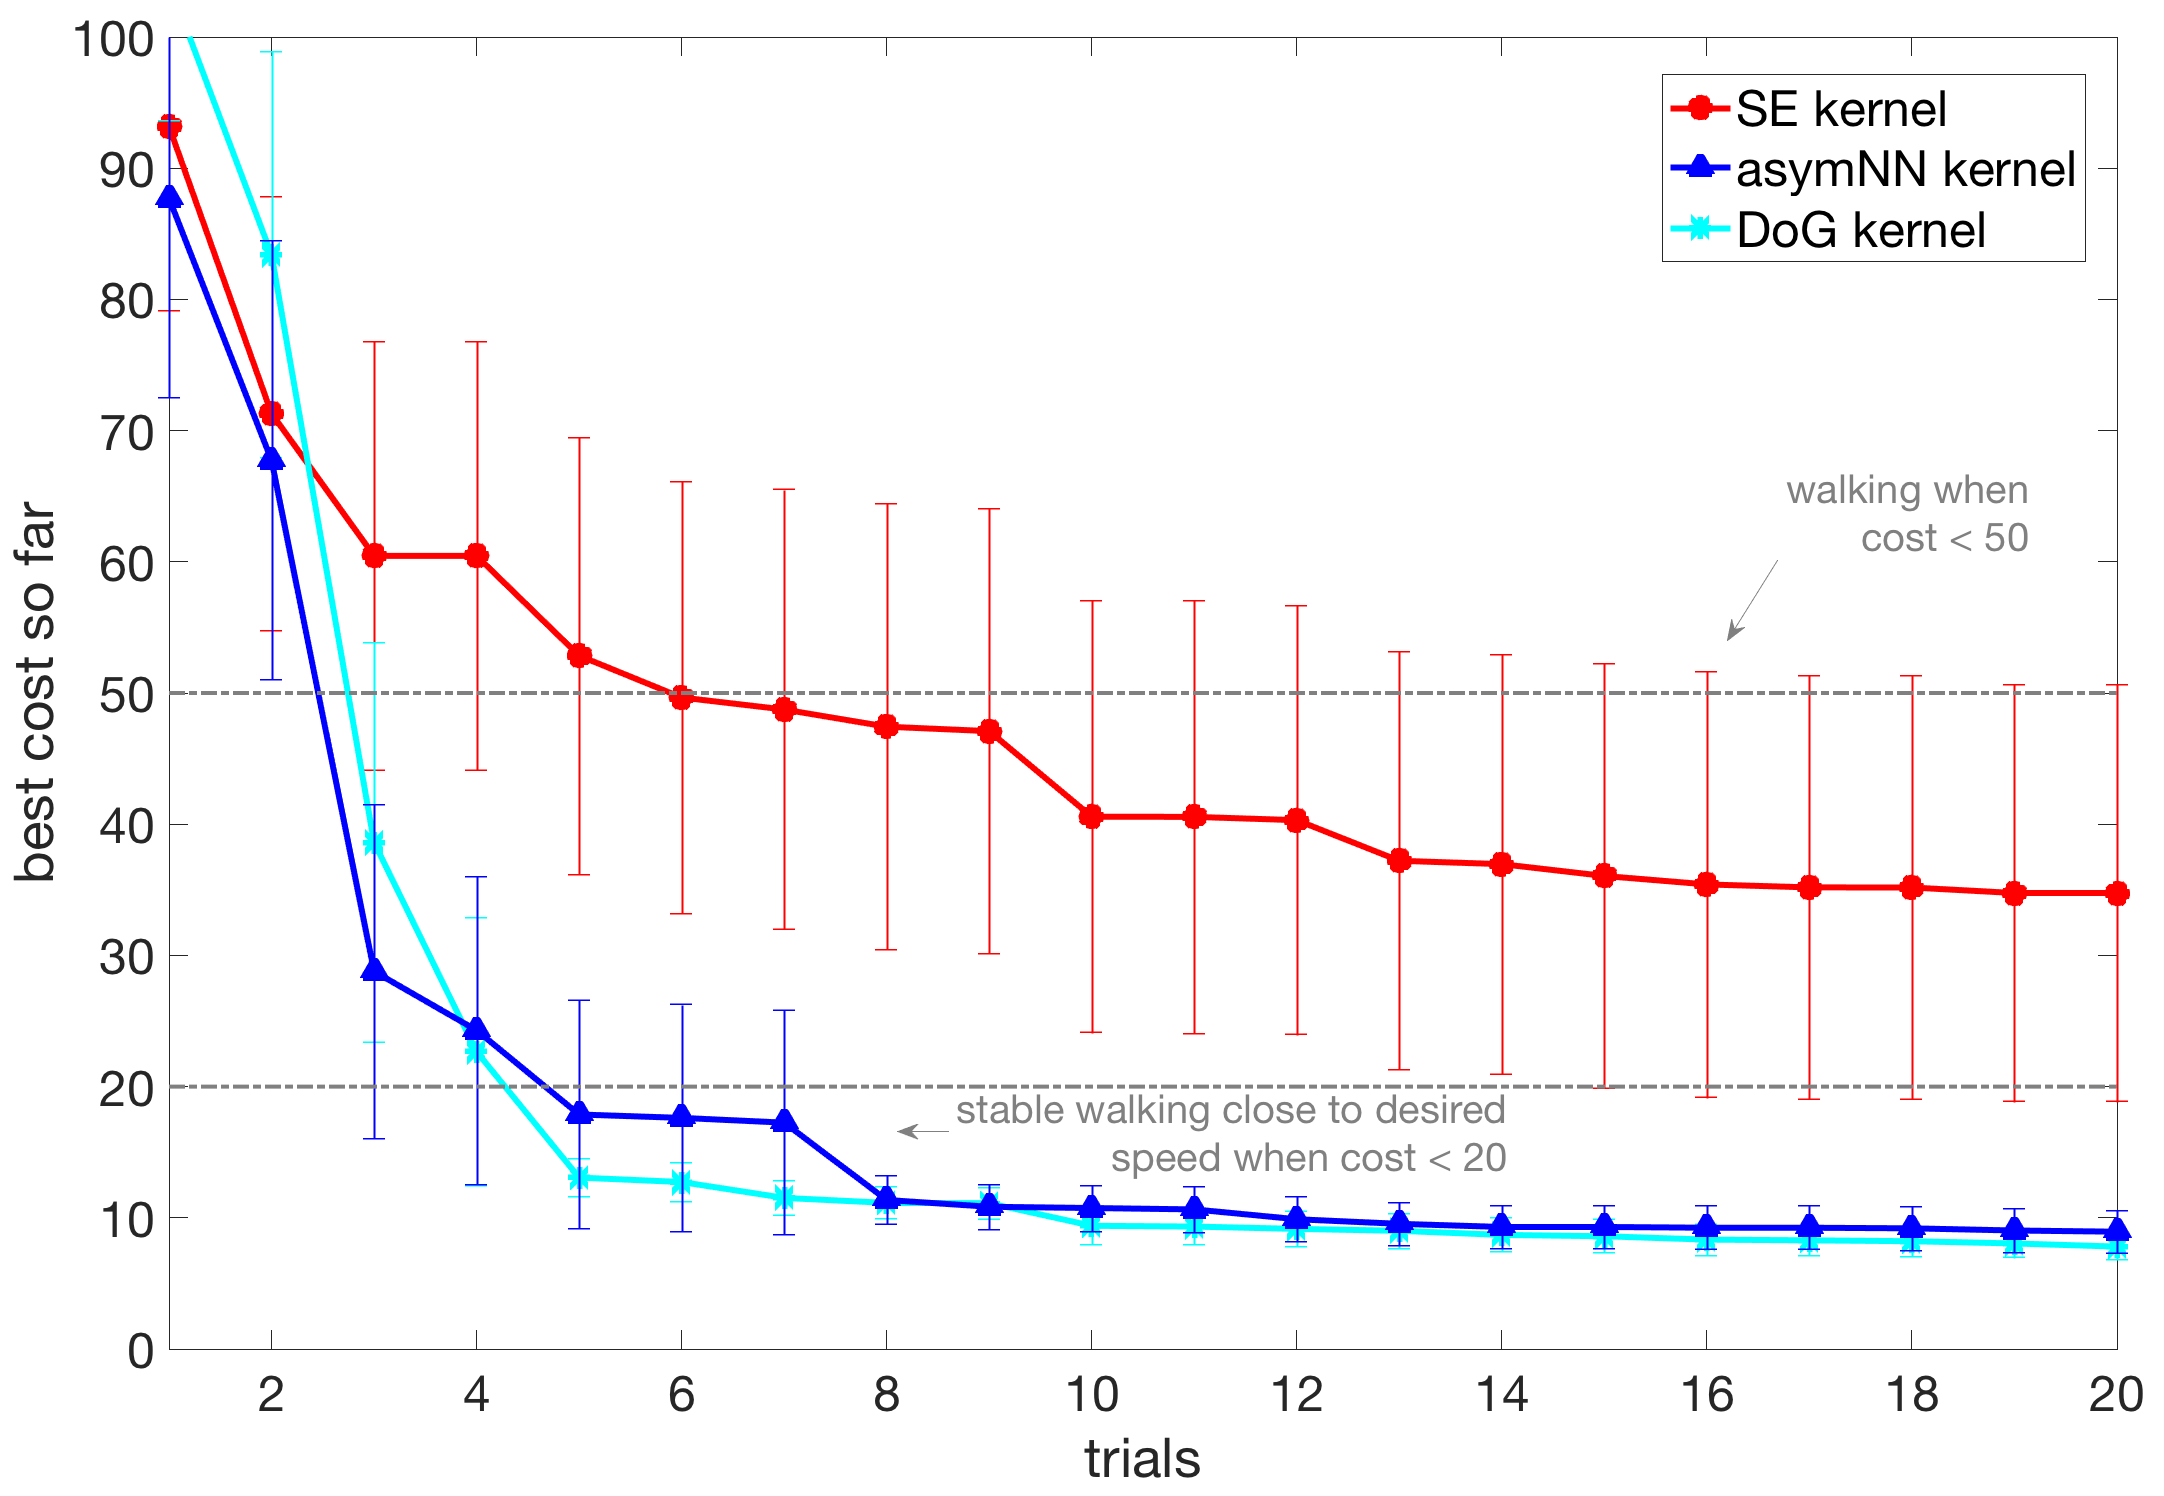
\includegraphics[width=0.8\textwidth]{img/nn_sftpl_vs_vanilla_BO_vs_DoG_kernels}
%\caption{\small{Initial tests in simulation.}}
%\label{fig:bo_runs_atrias_sim}
%\end{figure}

%In Figure~\ref{fig:bo_runs_atrias_sim} we first compare the performance of BO that used our neural network kernel (\textit{asymNN}) versus using a standard Squared Exponential kernel (\textit{SE}) in simulation. For these experiments we used the cost in Equation~\ref{eq:cost_atrias},  Section~\ref{sec:approach_asym} with a target velocity of $1m/s$. Simulations with cost less than 50 yielded walking behavior, while cost less than 20 resulted in a stable walk close to the desired speed. BO with \textit{asymNN} kernel was able to reliably find points corresponding to stable walking behavior in only 8 trials. In contrast, BO with \textit{SE} kernel did not find stable walking solutions in the first 20 trials reliably. We also compare with the \dogkernel kernel. \textit{asymNN} is able to closely match the performance of \dogkernel in this setting after 8 trials.

We sampled 100 random controllers with a target speed of $0.4m/s$ on hardware, and 16 controllers walked. A lower target speed meant that $\frac{1}{6}$ of the controller space was stable walking controllers. We completed 6 sets of runs of BO: 3 using \textit{asymNN} kernel and 3 using a standard \mbox{\textit{SE} kernel} with 10 trials each, leading to a \mbox{total of 60 hardware experiments}. Figure~\ref{fig:bo_runs_plot_atrias_hw} shows the performance of BO with SE versus \textit{asymNN} kernel. SE obtains a stable walking solution on the 3rd trial in one run, and on the 4th trial in the two other runs. \textit{asymNN} kernel is able to find the best-performing set of parameters on the second trial in each of the 3 runs. This confirms that using \textit{asymNN} kernel offers an improvement over using \textit{SE} kernel in this setting. We suggest that \textit{asymNN} reliably selects an excellent point on the 2nd trial  because such points lie far from  poorly performing subspace of parameters (under the distance metric constructed with \textit{asymNN}). 

While both SE kernel and \textit{asymNN} kernels perform very well in this setting, the \textit{asymNN} kernel is more biased towards sampling stable points than the SE kernel, as shown in Figure \ref{fig:bo_runs_plot_atrias_hw}. In the three runs, \textit{asymNN} kernel samples 23 stable controllers out of 30, while SE kernel samples 15 stable controllers. This implies that the search for optimal controllers is biased towards safety in the case of \textit{asymNN} kernel. This is desirable as stable points are less likely to break the robot.

\begin{figure}[t]
\centering
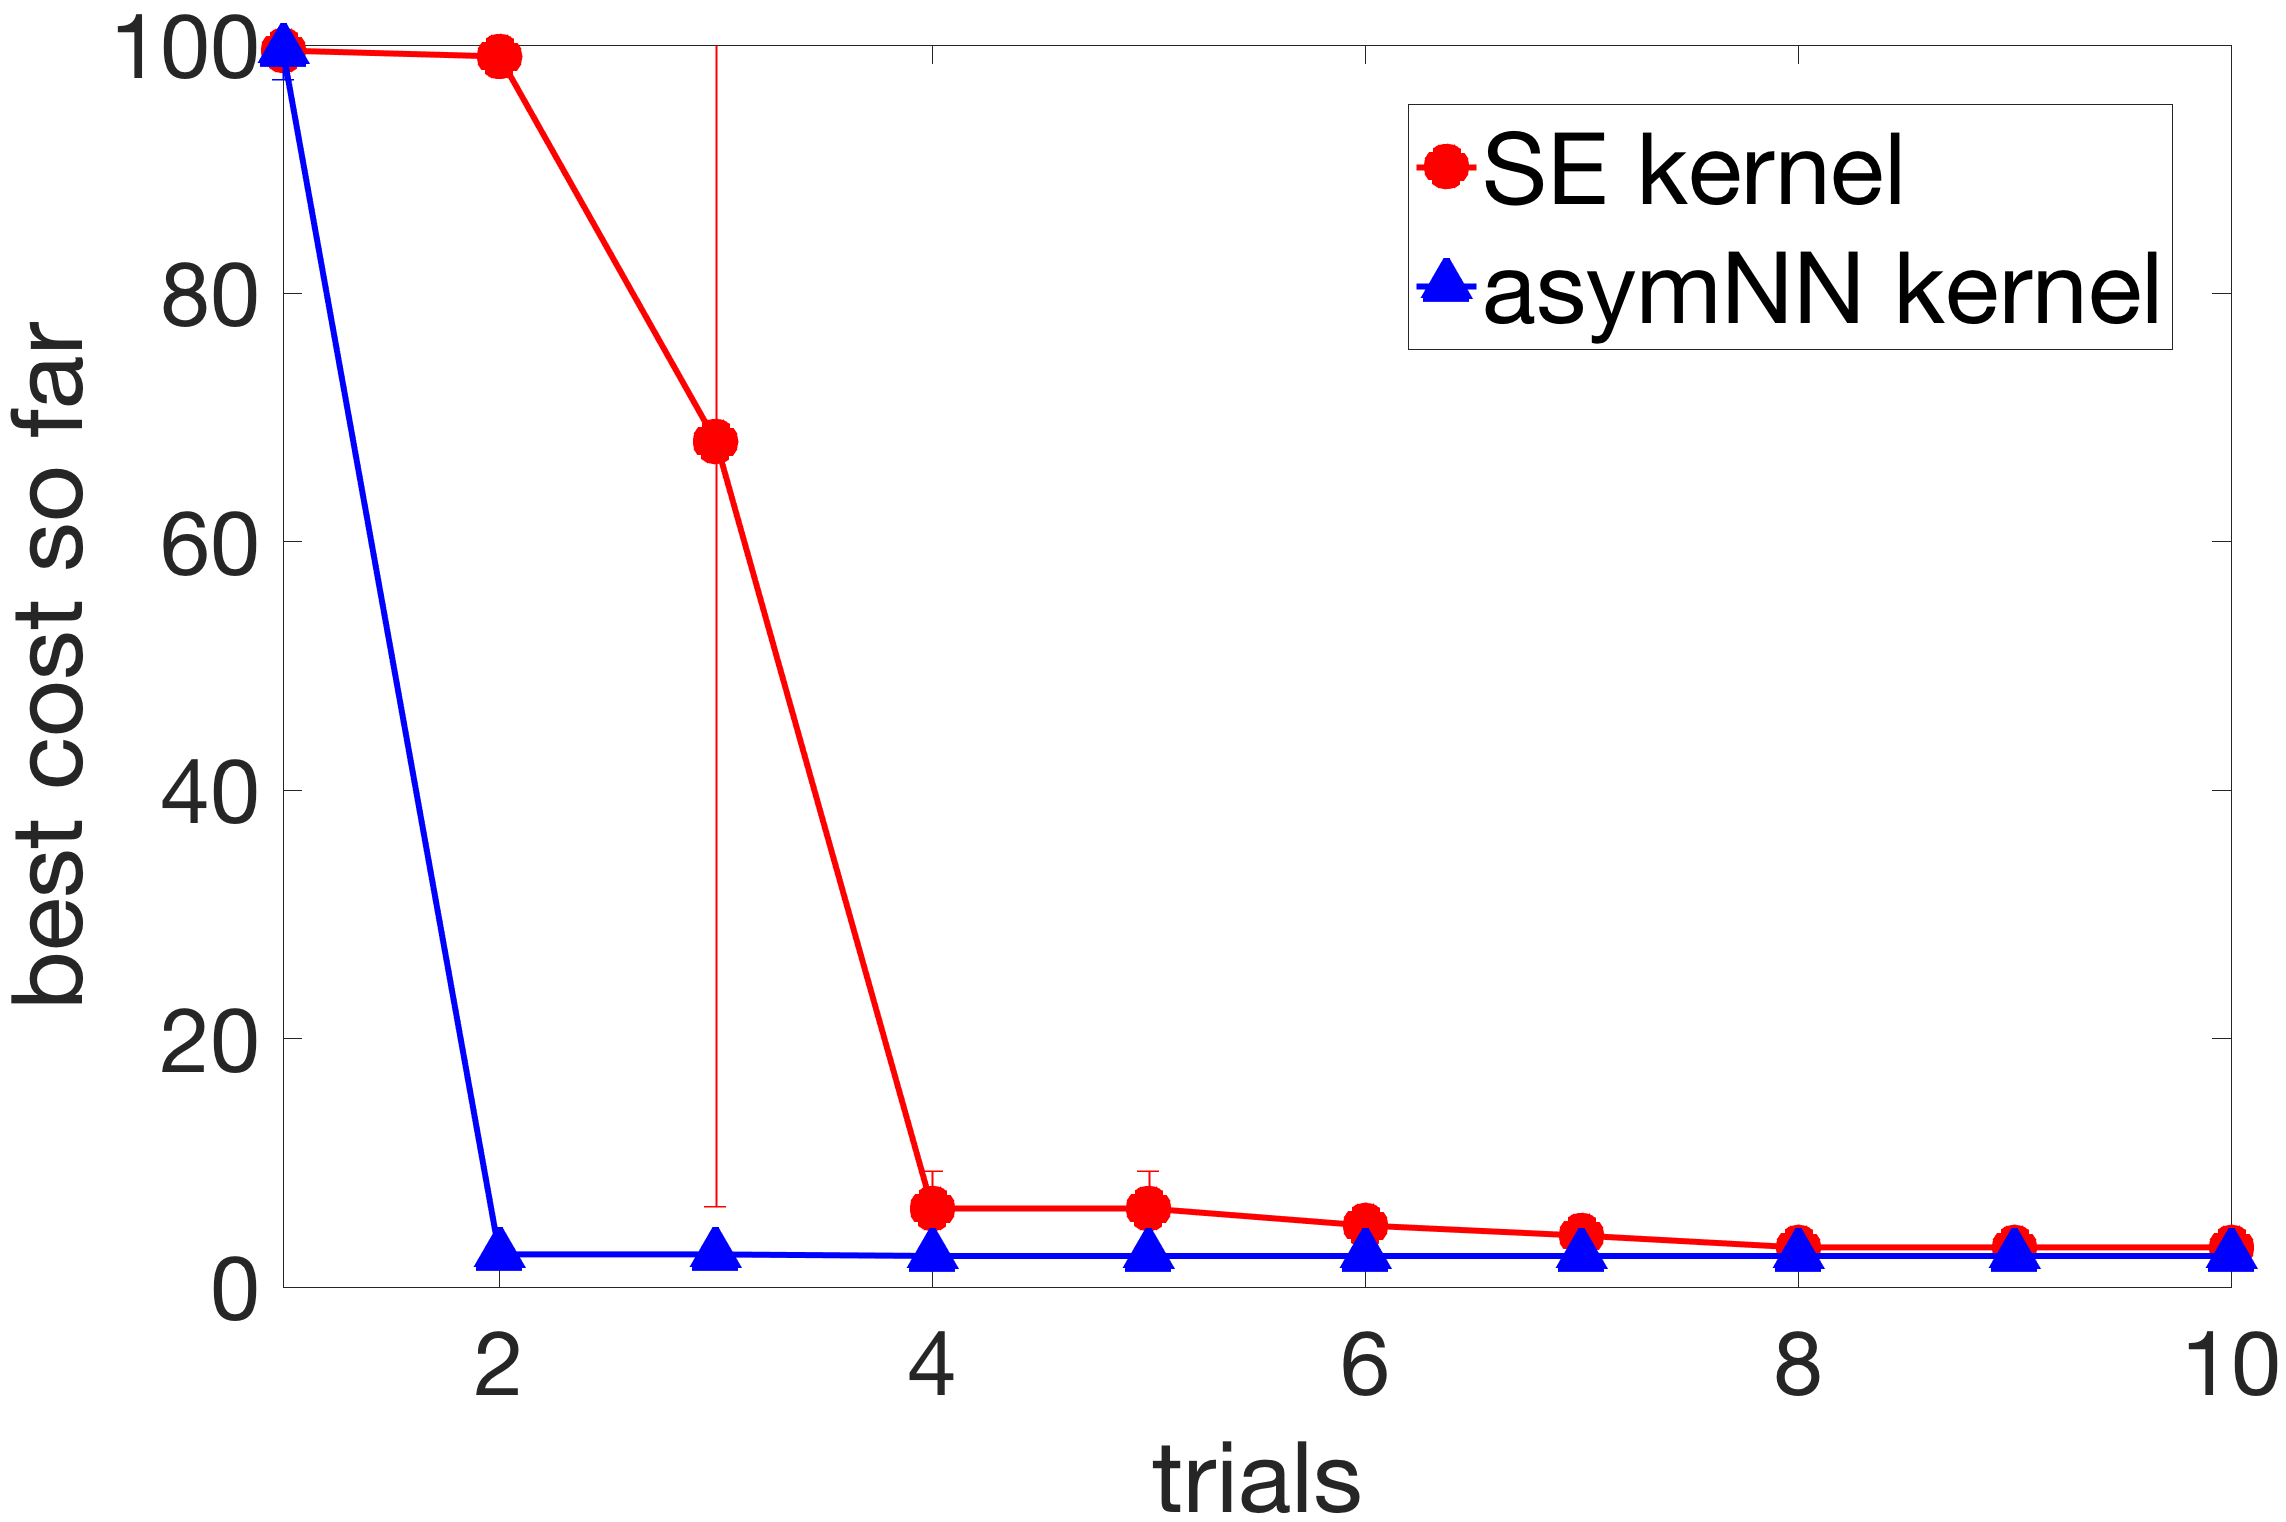
\includegraphics[width=0.43\textwidth]{img/hdw_runs.png}
\hspace{0.15cm}
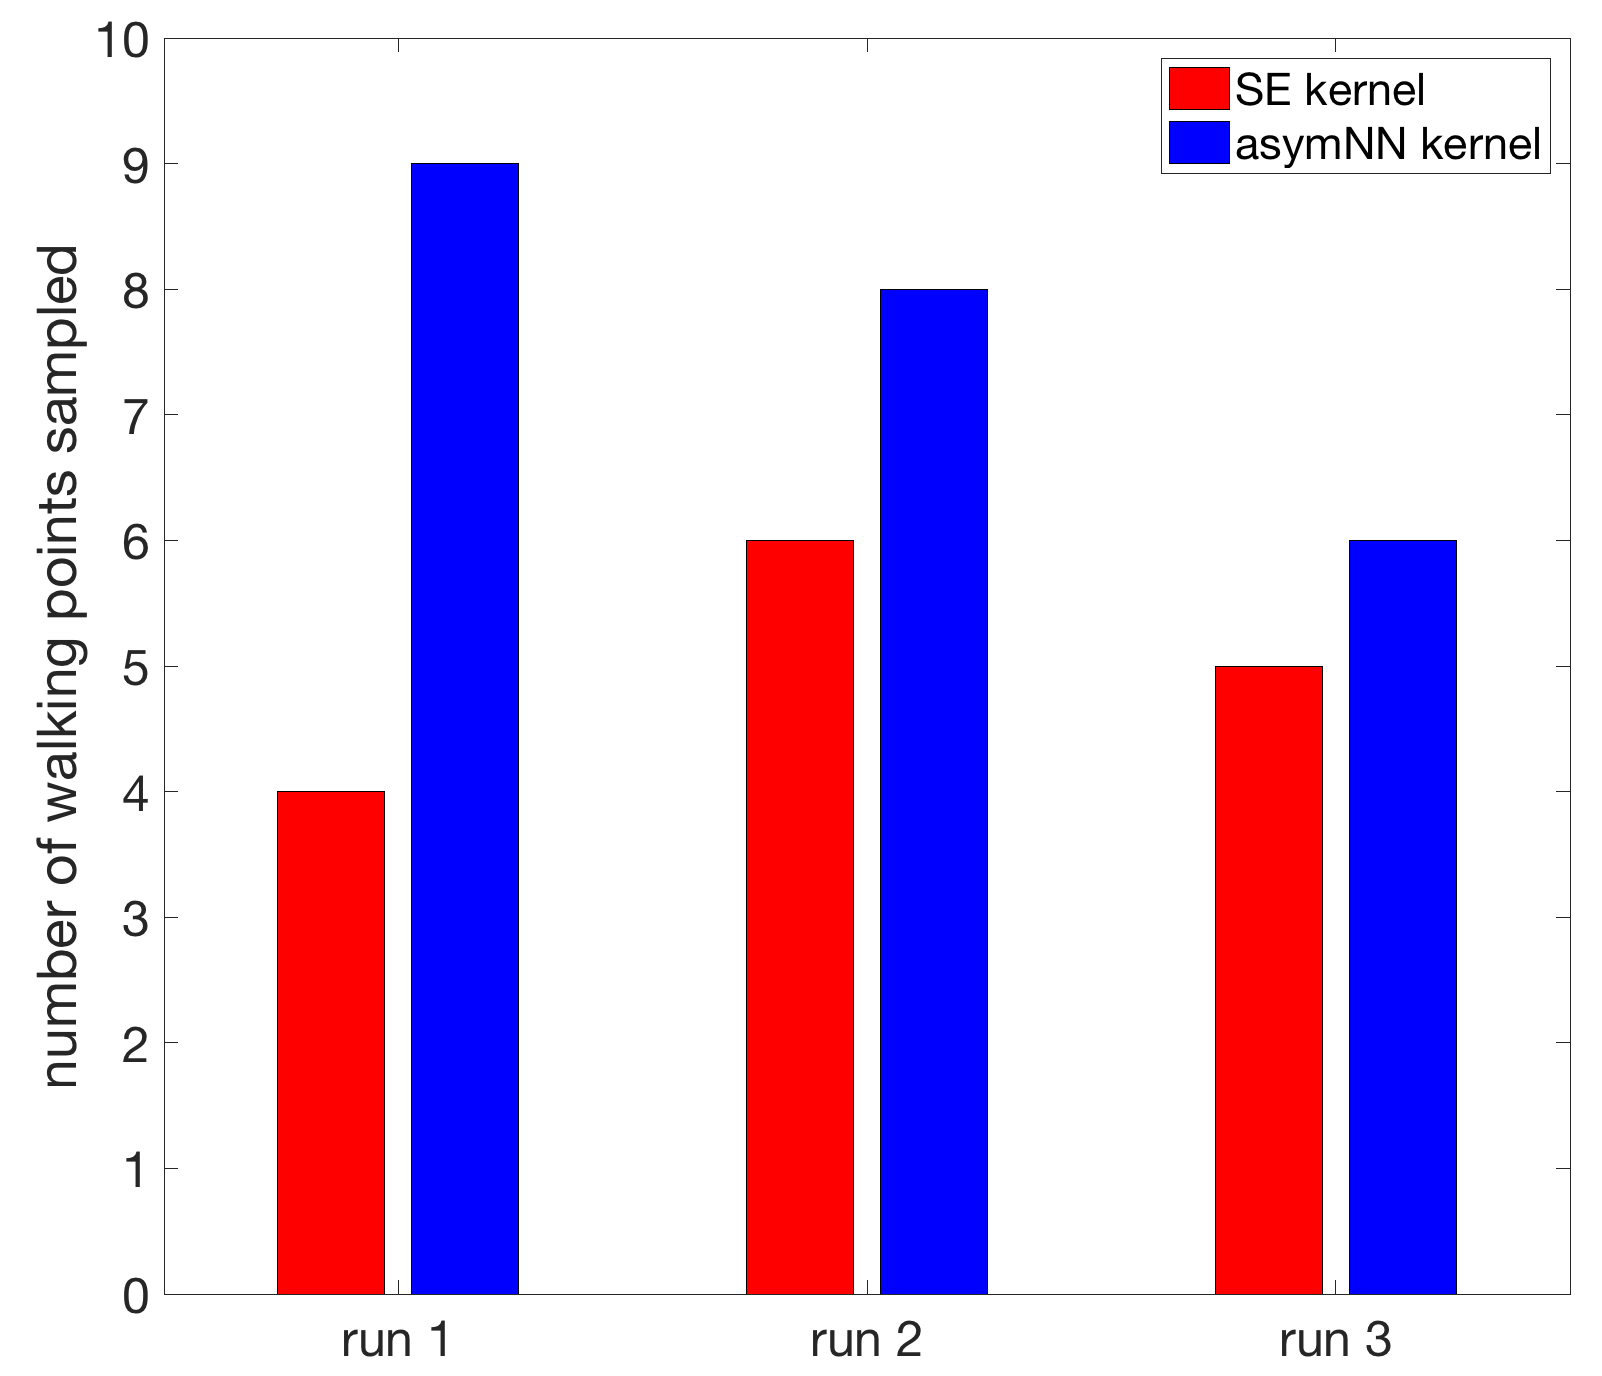
\includegraphics[width=0.43\textwidth]{img/walking_pts_sampled}
\caption{\small{(left) Best cost so far during BO (mean over 3 runs) for a target speed of $0.4m/s$. (right) Number of walking points sampled in each of the 3 runs.}}
\label{fig:bo_runs_plot_atrias_hw}
\end{figure}

On a more challenging, variable target speed profile of $0.4 m/s \text{ (15 steps)} - 1.0 m/s$ 
$$\text{ (15 steps)} - 0.2 m/s \text{ (15 steps)} - 0 m/s \text{ (5 steps)}$, the performance of the \textit{asymNN} kernel is slightly worse than the \dogkernel, though still better than SE kernel. Figure \ref{fig:no_nn_all_3} shows BO with  \textit{asymNN} kernel, SE kernel and \dogkernel for the variable speed profile. \dogkernel can find walking controllers in 2 trials in all 3 runs, while it takes \textit{asymNN} kernel 5 trials. On the other hand, SE kernel fails to reliably find controllers even after 20 trials.

\begin{figure}
    \centering
    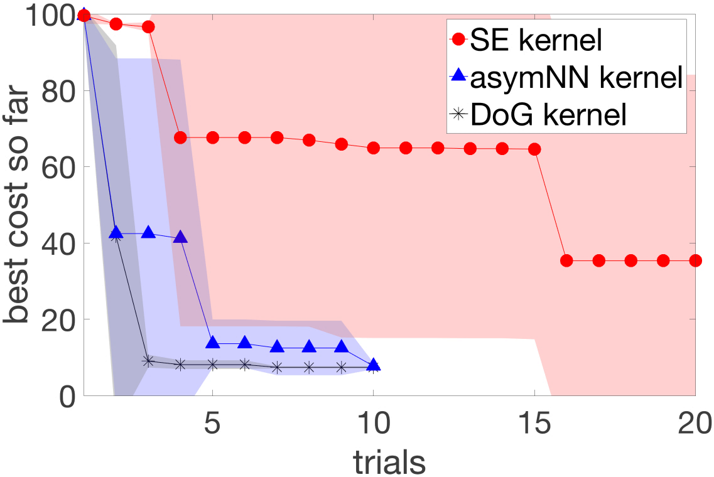
\includegraphics[width = 0.6\textwidth]{img/bo_nn_all_3.png}
    \caption{Bayesian optimization for a 5-dimensional controller with a variable target speed profile.}
    \label{fig:bo_nn_all_3}
\end{figure}


\begin{figure}[t]
\centering
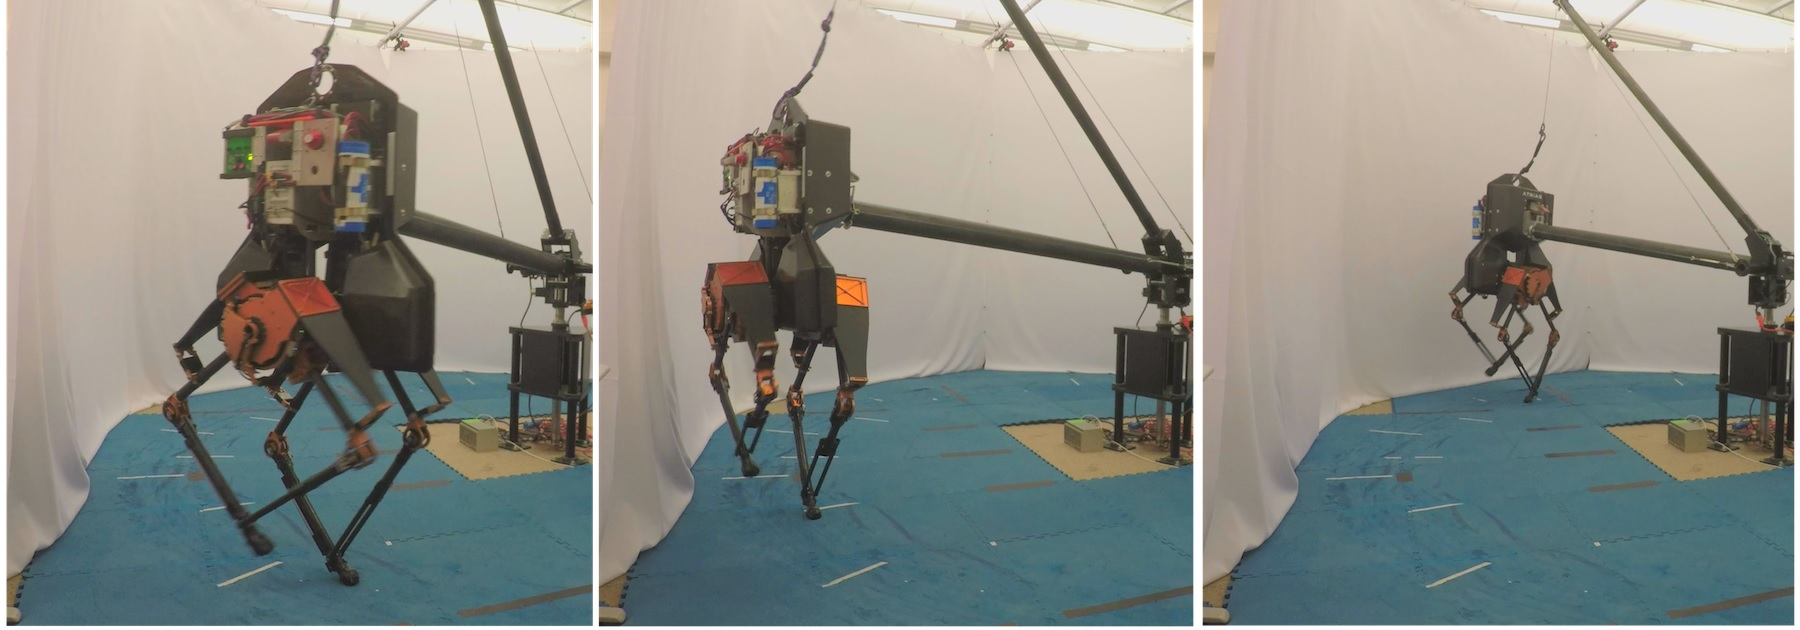
\includegraphics[width=0.8\textwidth]{img/atrias_walk_slides.jpg}
\caption{ATRIAS during BO with \textit{asymNN} kernel.}
\label{fig:bo_runs_atrias_hw_slides}
\end{figure}




While in our hardware setup most methods are likely to sample walking points within 10 trials, we believe our experimentation is an important step towards optimizing locomotion policies for complex humanoid robots. Bayesian Optimization studies in the past have also used real robot hardware, for example, \cite{Calandra2016}, \cite{cully2015robots} and \cite{tesch}.
However, \cite{tesch, lizotte2007automatic, cully2015robots} used robots which are statically stable for significant parts of their gait, making discontinuities in the cost function landscape less likely and in turn making the optimization easier. On the other hand, ATRIAS is a complex bipedal system which is likely to fall with unstable controllers due to point feet. \cite{Calandra2016} use a walking robot similar to ours. However, their controller parametrization is very different, and not widely used, unlike our inverse dynamics and force-based controller which is more modern and state-of-the-art \cite{kuindersma2016optimization}, \cite{herzog2016momentum}, \cite{feng2015optimization}. 

Hence, even if our policy parametrization was chosen so that steady walking points could be found in a few trials, our testbed is fairly complex and our problem formulation is widely applicable. 


\subsection{Hardware experiments with a 9-dimensional controller}

\begin{figure}
    \centering
    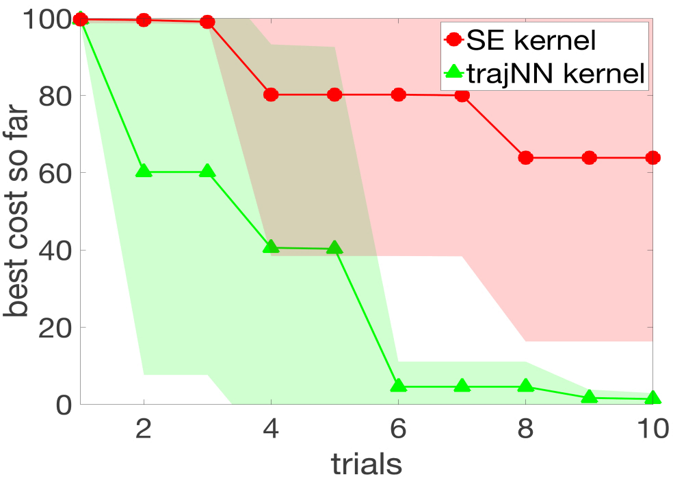
\includegraphics[width = 0.5\textwidth]{img/9d_hdw_nn.png}}
    \caption{Bayesian optimization of a 9-dimensional kernel with the NN-based kernel.}
    \label{fig:9d_hdw_nn}
\end{figure}
In the next set of experiments, we evaluated performance of the NN-based kernel described in Section~\ref{subsec:proposed_traj_nn}. We optimize the 9-dimensional controller from Section \ref{subsec:raibert_cont}. 

The target of hardware experiments was to walk for 30 steps at $0.4m/s$, similar to Section \ref{subsec:dog-9d}. We observed that the SE performance was slightly better as compared to the old experiments, even though starting from the same random samples, hyper-parameter setting and speed profile. We attribute this change to a better estimation and control of the CoM vertical height, owing to a new IMU on the robot. 


Figure~\ref{fig:9d_hdw_nn} shows comparison of BO with NN-based kernel and SE kernels. We conducted 5 runs of both algorithms with 10 trials in each run, leading to a total of 100 robot trials. BO with the NN-based kernel found walking points in all 5 runs within 6 trials, while BO with SE kernel only found walking points in 2 of 5 runs in 10 trials.
Hence, even without explicit hand-designed domain knowledge, like the \dogkernel kernel, the NN-based kernel is able to extract useful information from simulation and successfully guide hardware experiments.


\subsection{Simulation experiments with the 16-dimensional controller}
\label{experiments_nm}

In section~\ref{sec:approach_traj} we introduced a cost-agnostic approach for constructing an informed kernel from simulations. Our approach is to train a neural network to reconstruct trajectory information. In this Section, we describe our experiments with 16-dimensional controller of the Neuromuscular model on a 7-link biped. We created a grid of 100K points in the input parameter space  and ran short 5 second simulations on each of the corresponding 100K parameter sets to collect the trajectory summaries. We then used a fully connected network with 4 hidden layers (512, 128, 32 units) with L1 loss to reconstruct the summaries of the trajectories (as described in section~\ref{sec:approach_traj}). This transformation induced by the neural network was used as a re-parameterization from the input space of 16-dimensional controller parameters to 8-dimensional space of trajectory summaries. These 8-dimensional outputs of the neural network define kernel distances in the informed kernel (\textit{trajNN}). All experiments were conducted on perturbed models, as described in Section \ref{sec:probform}.

Figures~\ref{fig:smooth_cost_bo_runs}, \ref{fig:nonsmooth_cost_bo_runs} illustrate our experiments comparing using \textit{trajNN} versus using Squared Exponential (\textit{SE}) kernel for BO. To analyze the performance of \textit{trajNN} on different cost functions we conducted experiments on two different costs suggested in prior literature. The first cost promotes walking further and longer before falling, while penalizing deviations from the target speed~\citep{rai2016sample}:
\begin{equation}
cost_{smooth} = 1/(1+t) + 0.3/(1+d) + 0.01(v-v_{tgt}),
\label{eq:cost_smooth}
\end{equation}
where $t$ is seconds walked, $d$ is the final hip position, $v$ is mean velocity and $v_{tgt}$ is the desired walking velocity ($1.3m/s$ in our case). 
The second cost function is a simplified version of the cost used in~\cite{song2015neural}, penalizes falls explicitly, and encourages walking at desired speed and with lower cost of transport:
\begin{equation}
cost_{non\text{-}smooth} = 		
    \begin{cases}
		300 - x_{fall} , \text{\small{if fall}} \\
		100 ||v_{avg} - v_{tgt}|| + c_{tr}, \text{\small{if walk}}\\
	\end{cases}
\label{eq:cost_nonsmooth}
\end{equation}
where $x_{fall}$ is the distance covered before falling, $v_{avg}$ is the average speed of walking, $v_{tgt}$ is the target velocity, and $c_{tr}$ captures the cost of transport.

Figure~\ref{fig:smooth_cost_bo_runs} shows that \textit{trajNN} offers a significant improvement in sample efficiency when using $cost_{smooth}$ during optimization. Points with cost less than $0.15$ correspond to robust walking behavior. With \textit{trajNN}, more than $90\%$ of runs obtain walking solutions after only 25 trials. In contrast, using \textit{SE} requires more than 90 trials for such success rate. The performance of \textit{trajNN} matches that of a \dogkernel kernel. This is notable, since \textit{trajNN} is learned automatically, whereas \dogkernel kernel is constructed using domain expertise.


\begin{figure}[t]
\centering
\caption{Optimizing smooth cost from Equation~\ref{eq:cost_smooth} over 50 runs.}
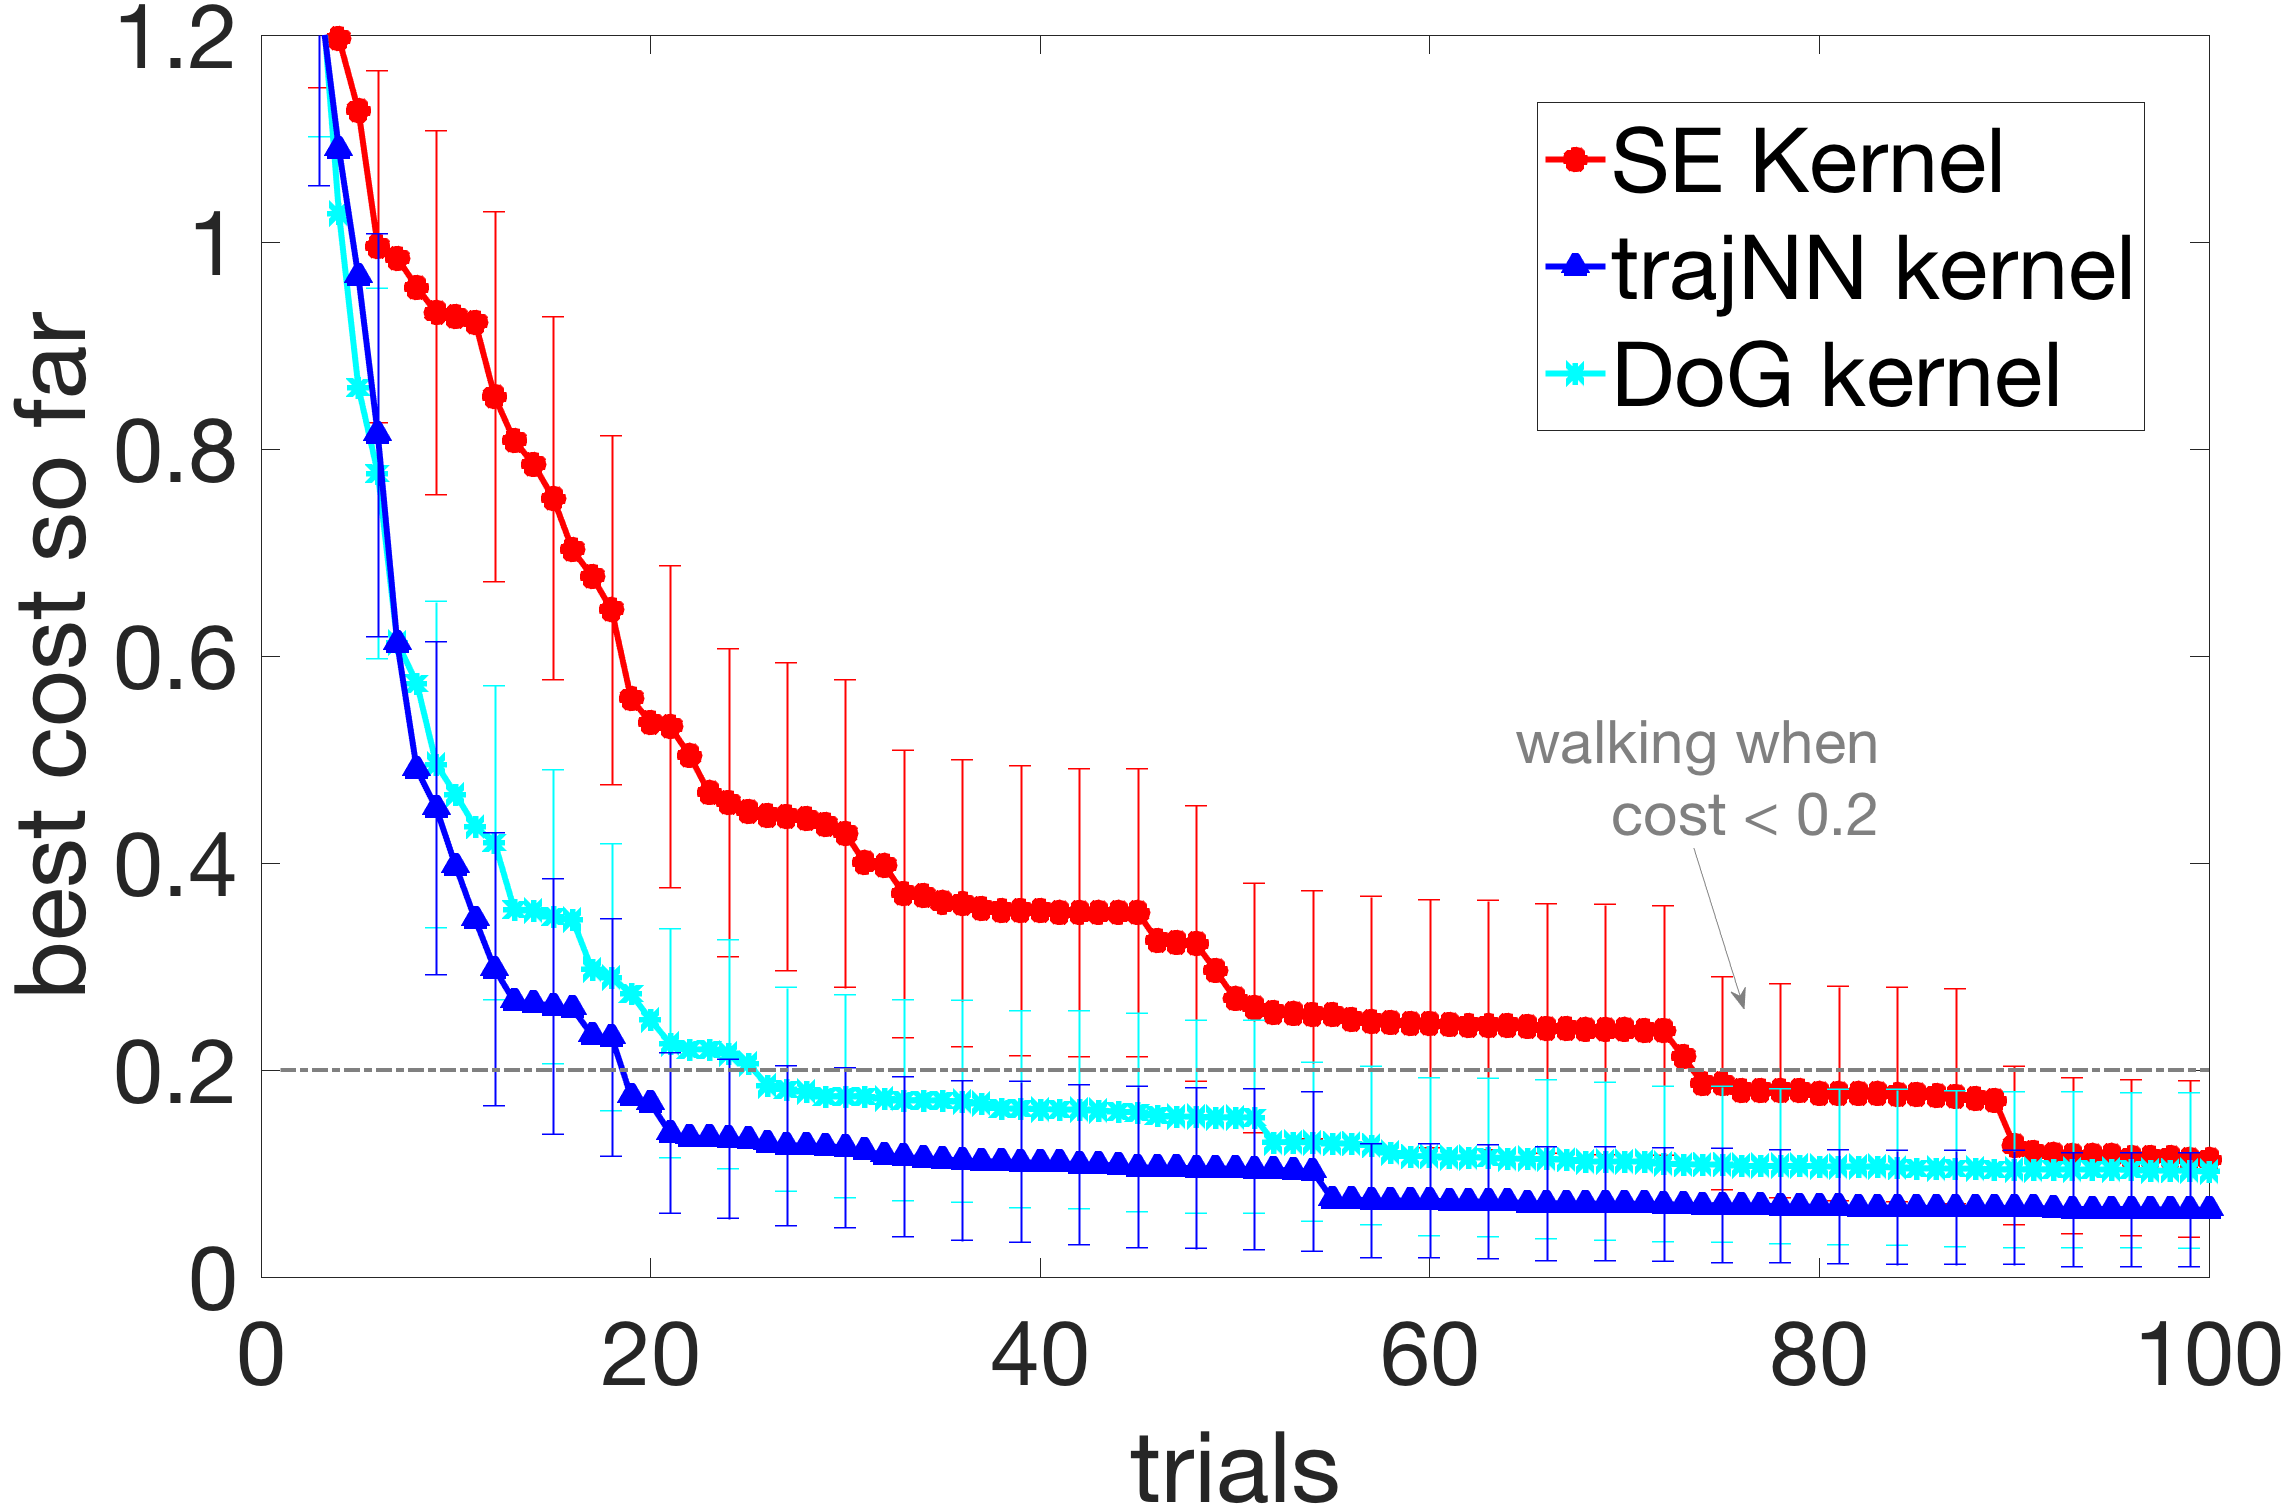
\includegraphics[width=0.65\textwidth]{img/smooth_cost_bo_runs}
\label{fig:smooth_cost_bo_runs}
\end{figure}

\begin{figure}[t]
\centering
\caption{Optimizing non-smooth cost from Equation~\ref{eq:cost_nonsmooth} over 50 runs.}
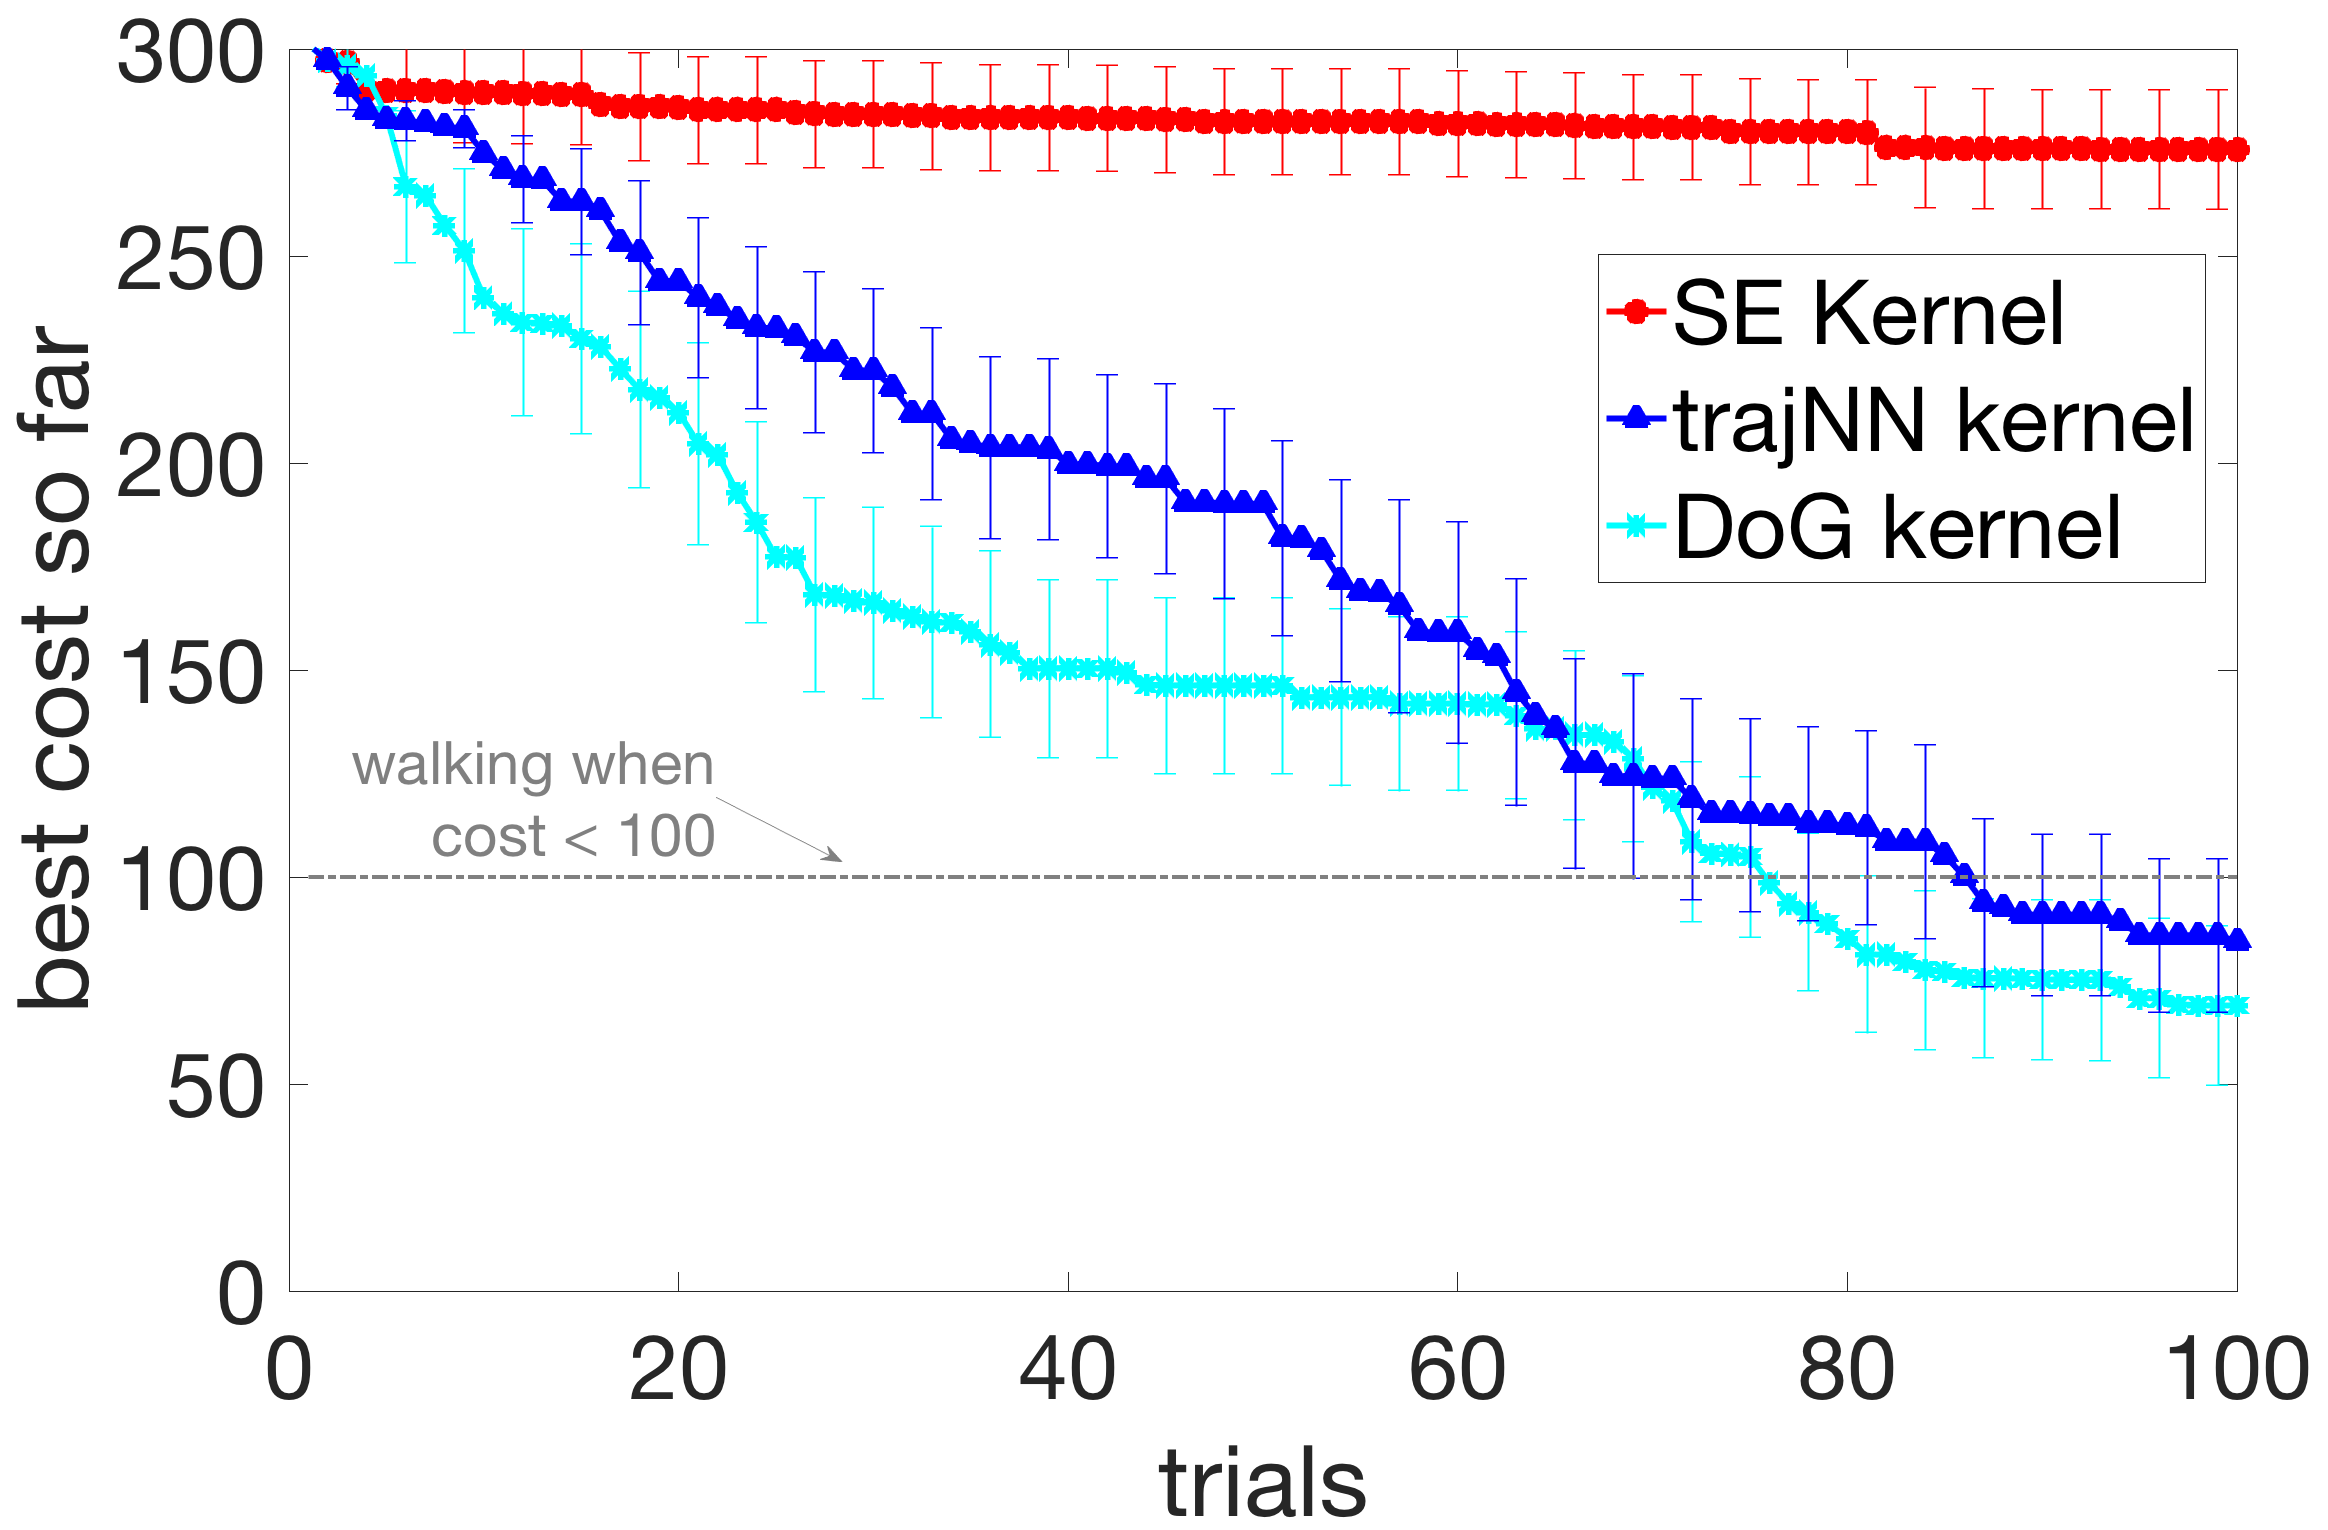
\includegraphics[width=0.65\textwidth]{img/nonsmooth_cost_bo_runs}
\label{fig:nonsmooth_cost_bo_runs}
\end{figure}

Figure~\ref{fig:nonsmooth_cost_bo_runs} shows that \textit{trajNN} also provides a significant improvement when using the second cost. Points with cost less than $100$ correspond to walking. With \textit{trajNN}, 70\% of the runs find walking solutions after 100 trials. In contrast, optimizing non-smooth cost is very challenging for BO with \textit{SE} kernel: a walking solution is found only in 1 out of 50 runs after 100 trials.

The difference in performance on the two costs is due to the nature of the two costs. If a point walks some distance $d$, Equation \ref{eq:cost_smooth} penalizes points according to $1/d$ and Equation \ref{eq:cost_nonsmooth} penalizes them according to $-d$. This results in a much steeper fall in cost with the first cost, and BO starts to exploit around points that walk some distance, quickly finding points that walk forever. However, with the second cost, BO continues to explore, and sometimes does not find walking points even in 100 trials. Exploitative methods might be better suited for higher dimensional problems, as compared to exploratory methods, in our experience. 

\textit{trajNN} kernel might be preferable to a cost-based kernel not only for settings with multiple costs. For some higher dimensional problems reduction to a 1-dimensional space in the kernel could be undesirable. So, while 1-dimensional cost-based kernel could yield highly sample-efficient optimization for lower dimensional problems, a higher-dimensional kernel like \textit{trajNN} could provide more flexibility without compromising sample-efficiency for higher dimensional problems.

\subsection{Simulation experiments with 50-dimensional controller}

\begin{figure}
    \centering
    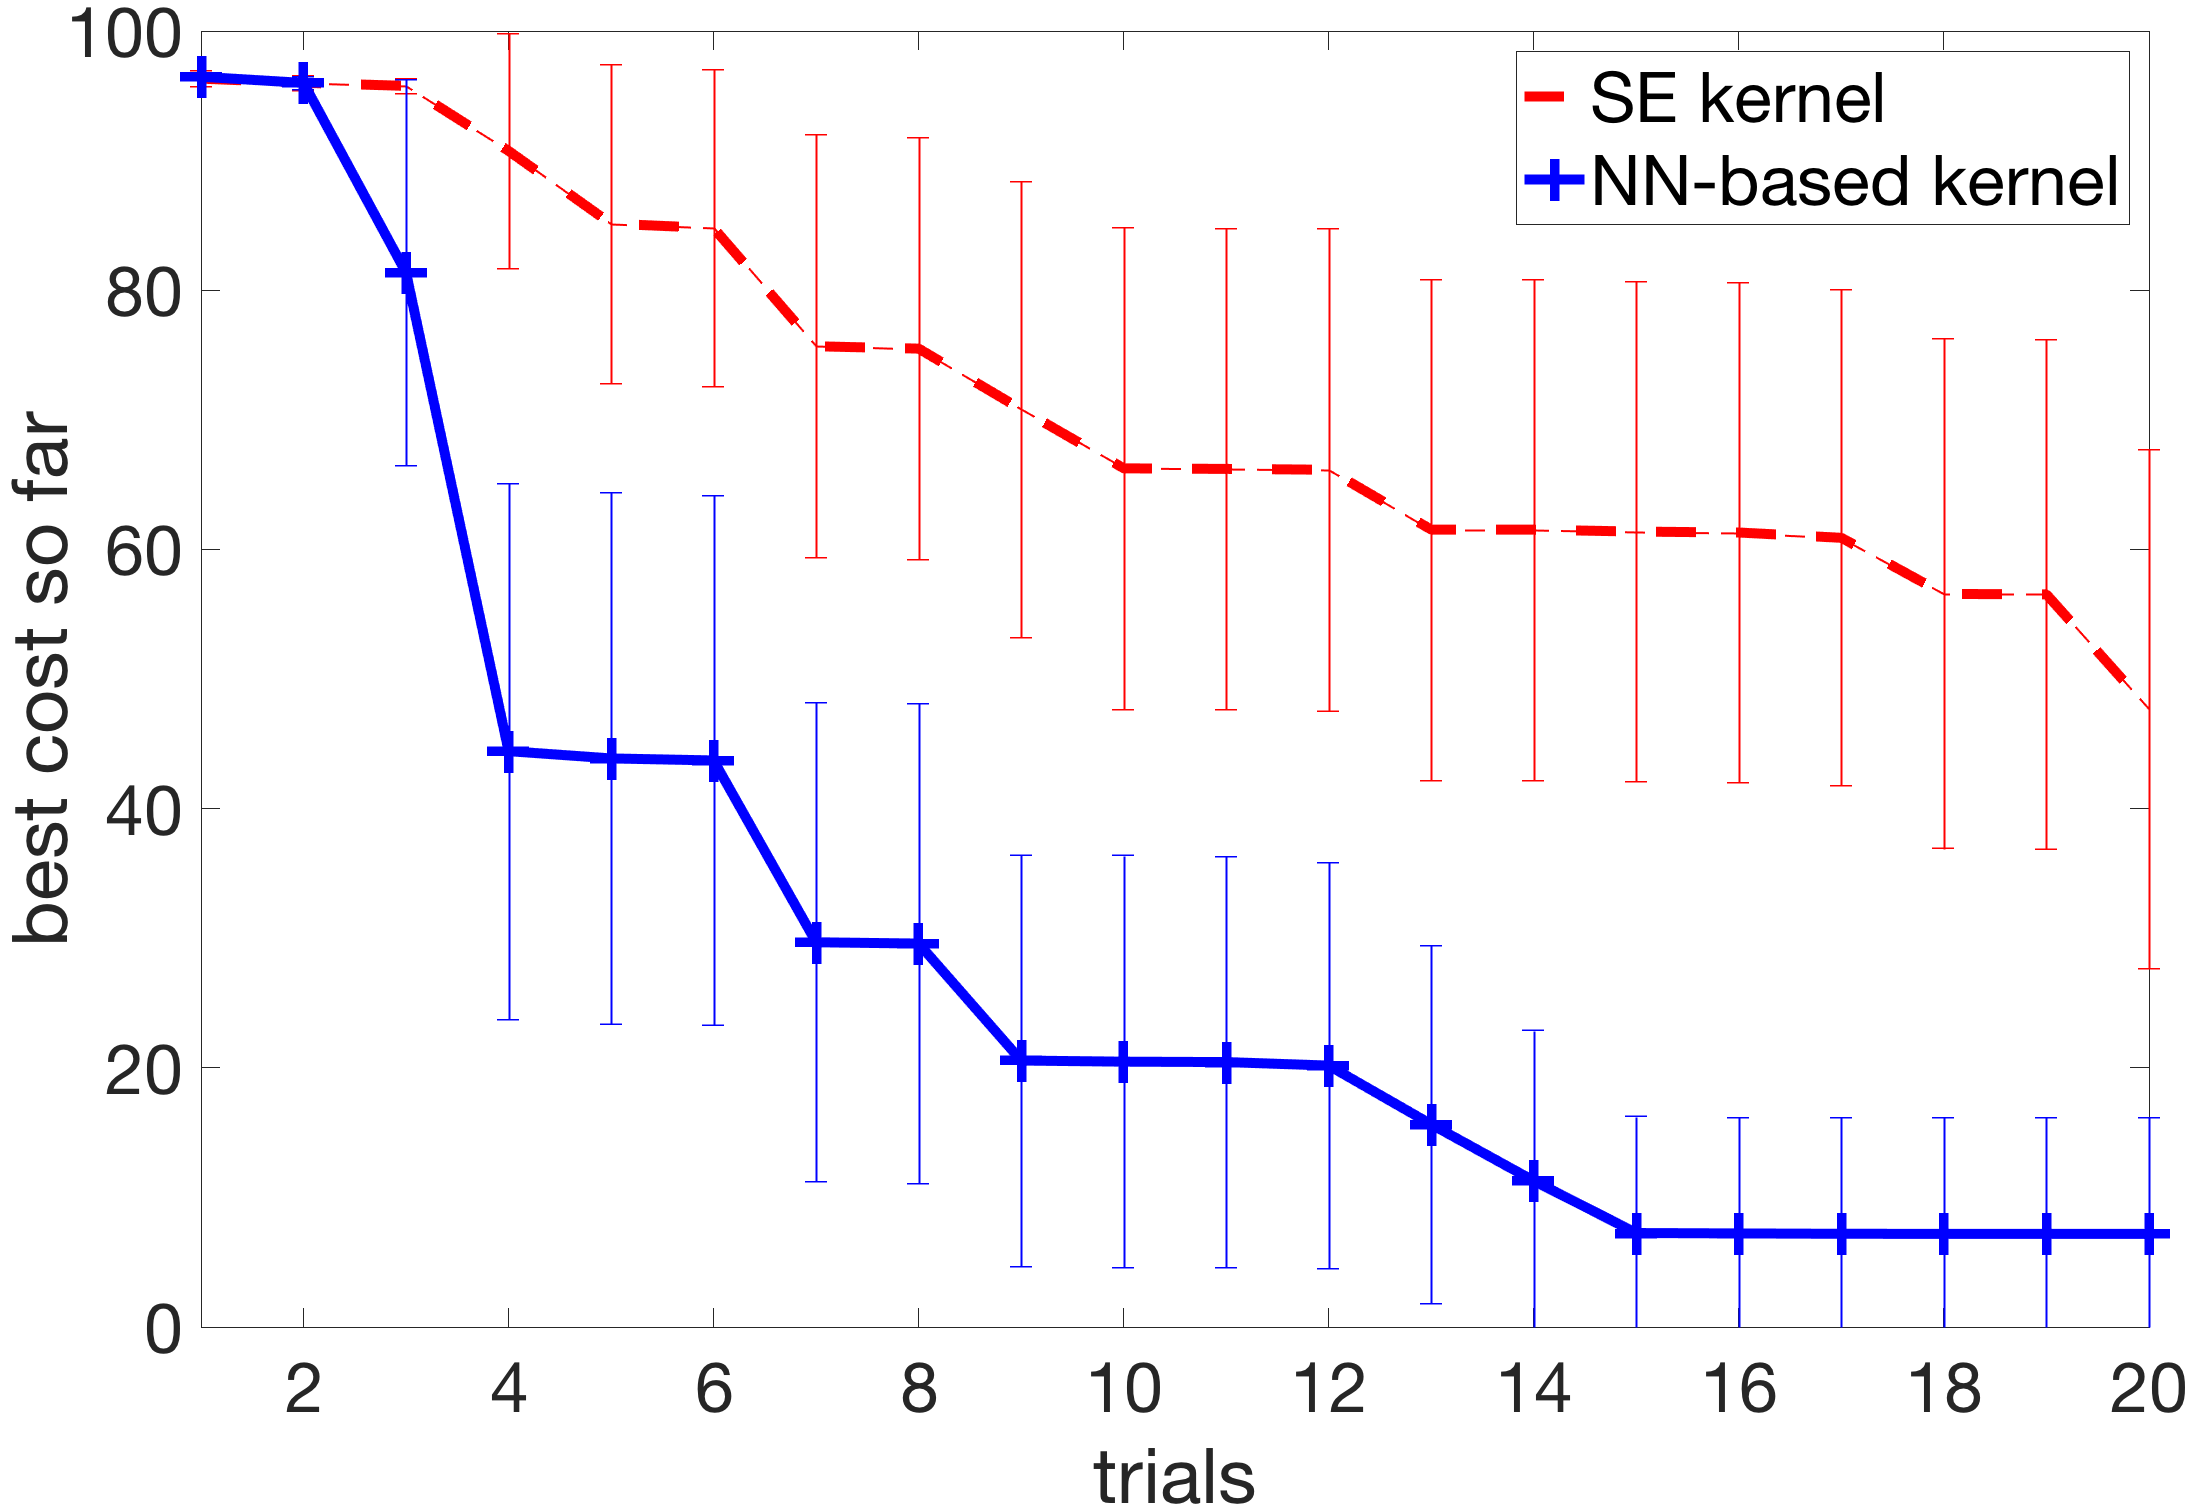
\includegraphics[width = 0.5\textwidth]{img/NN4_20runs_250K_holdout.png}}
    \caption{50-dimensional controller with a trajNN kernel in simulation.}
    \label{fig:nn4_vnmc}
\end{figure}

Our last set of simulation experiments were on the 50-dimensional controller, with the same experimental setting as Section \ref{}. The neural network kernel was trained to reconstruct the summaries of simulation trajectories over 200,000 simulation controllers. As can be seen in Figure \ref{fig:nn4_vnmc}, BO with NN-based kernel was able to find walking controllers in 20 trials in $95\%$ of the runs. This performance is similar to \dogkernel which can find walking controllers in 20 trials for $100\%$ of the runs. 

These results show that while the NN-based kernel uses lesser domain specific information than \dogkernel, its performance in simulation and hardware is very comparable to \dogkernel. As an additional advantage, the weights of the NN-based kernel can be learned from data experienced on hardware, by continuing to do gradient descent. This leads to a simple and straight-forward way of updating the kernel from hardware experiments. 

A summary of results and experimental settings described in the previous section is below:

\begin{table}[h!]
\centering
\ra{1.3}
\small{
\begin{tabular}{ lccccc } 
\toprule
Kernel & Controller & Number of & Sim & Kernel & Features \\
type & dimension & sim points & duration & dim & in kernel \\
\midrule
$k_{DoG}$ & 5 & 20K & 3.5s & 1 & $score_{DoG}$ \\ 
          & 9 & 100K & 5s & 1 & $score_{DoG}$ \\ 
     & 50 & 200K & 5s & 1 & $score_{DoG}$ \\ 
\hline
$k_{\textit{trajNN}}$ & 9 & 100K & 5s & 4 & $t_{walk}$, $x_{end}$, $\theta_{avg}$, $v_{x,avg}$\\ 
                      & 16 & 100K & 5s & 8 &
                $t_{walk}$, $x_{end}$, $\theta_{end}$, $v_{x,end}$\\
                & & & & & $c_{\tau}$,  $y_{end}$,  $v_{y,end}$, $\dot{\theta}_{end}$ \\ 
                      & 50 & 200K & 5s & 13 & $t_{walk}$, $x_{end}$, $c_{\tau}$, $\pmb{\textit{traj}}_{x}$, $\pmb{\textit{traj}}_{\theta}$ \\ 
\bottomrule
\end{tabular}
}
\caption{Simulation Data Collection Details. $score_{DoG}$ was described in Section \ref{subsec:proposed_dog_transform}. For $k_{\textit{trajNN}}$: $t_{walk}$ is time walked in simulation before falling, $x_{end}$ and $y_{end}$ are the $x$ and $y$ positions of Center of Mass (CoM) at the end of the short simulation, $\theta$ is the torso angle, $\dot{\theta}$ is the torso velocity, $v$ is the CoM speed ($v_{x}$ is the horizontal and $v_y$ is the vertical component), $c_{\tau}$ is the squared sum of torques applied; $\pmb{\textit{traj}}_{x}$, $\pmb{\textit{traj}}_{\theta}$ denote vectors with mean CoM and $\theta$ measurements every second.}
\label{tbl:kernel_details}
\end{table}


\AR{Add an overview table from experiments in this section.}


\section{Effect of inaccurate simulations on the performance}

\label{subsec:mismatch_experiments}

%\begin{figure}
%\centering
%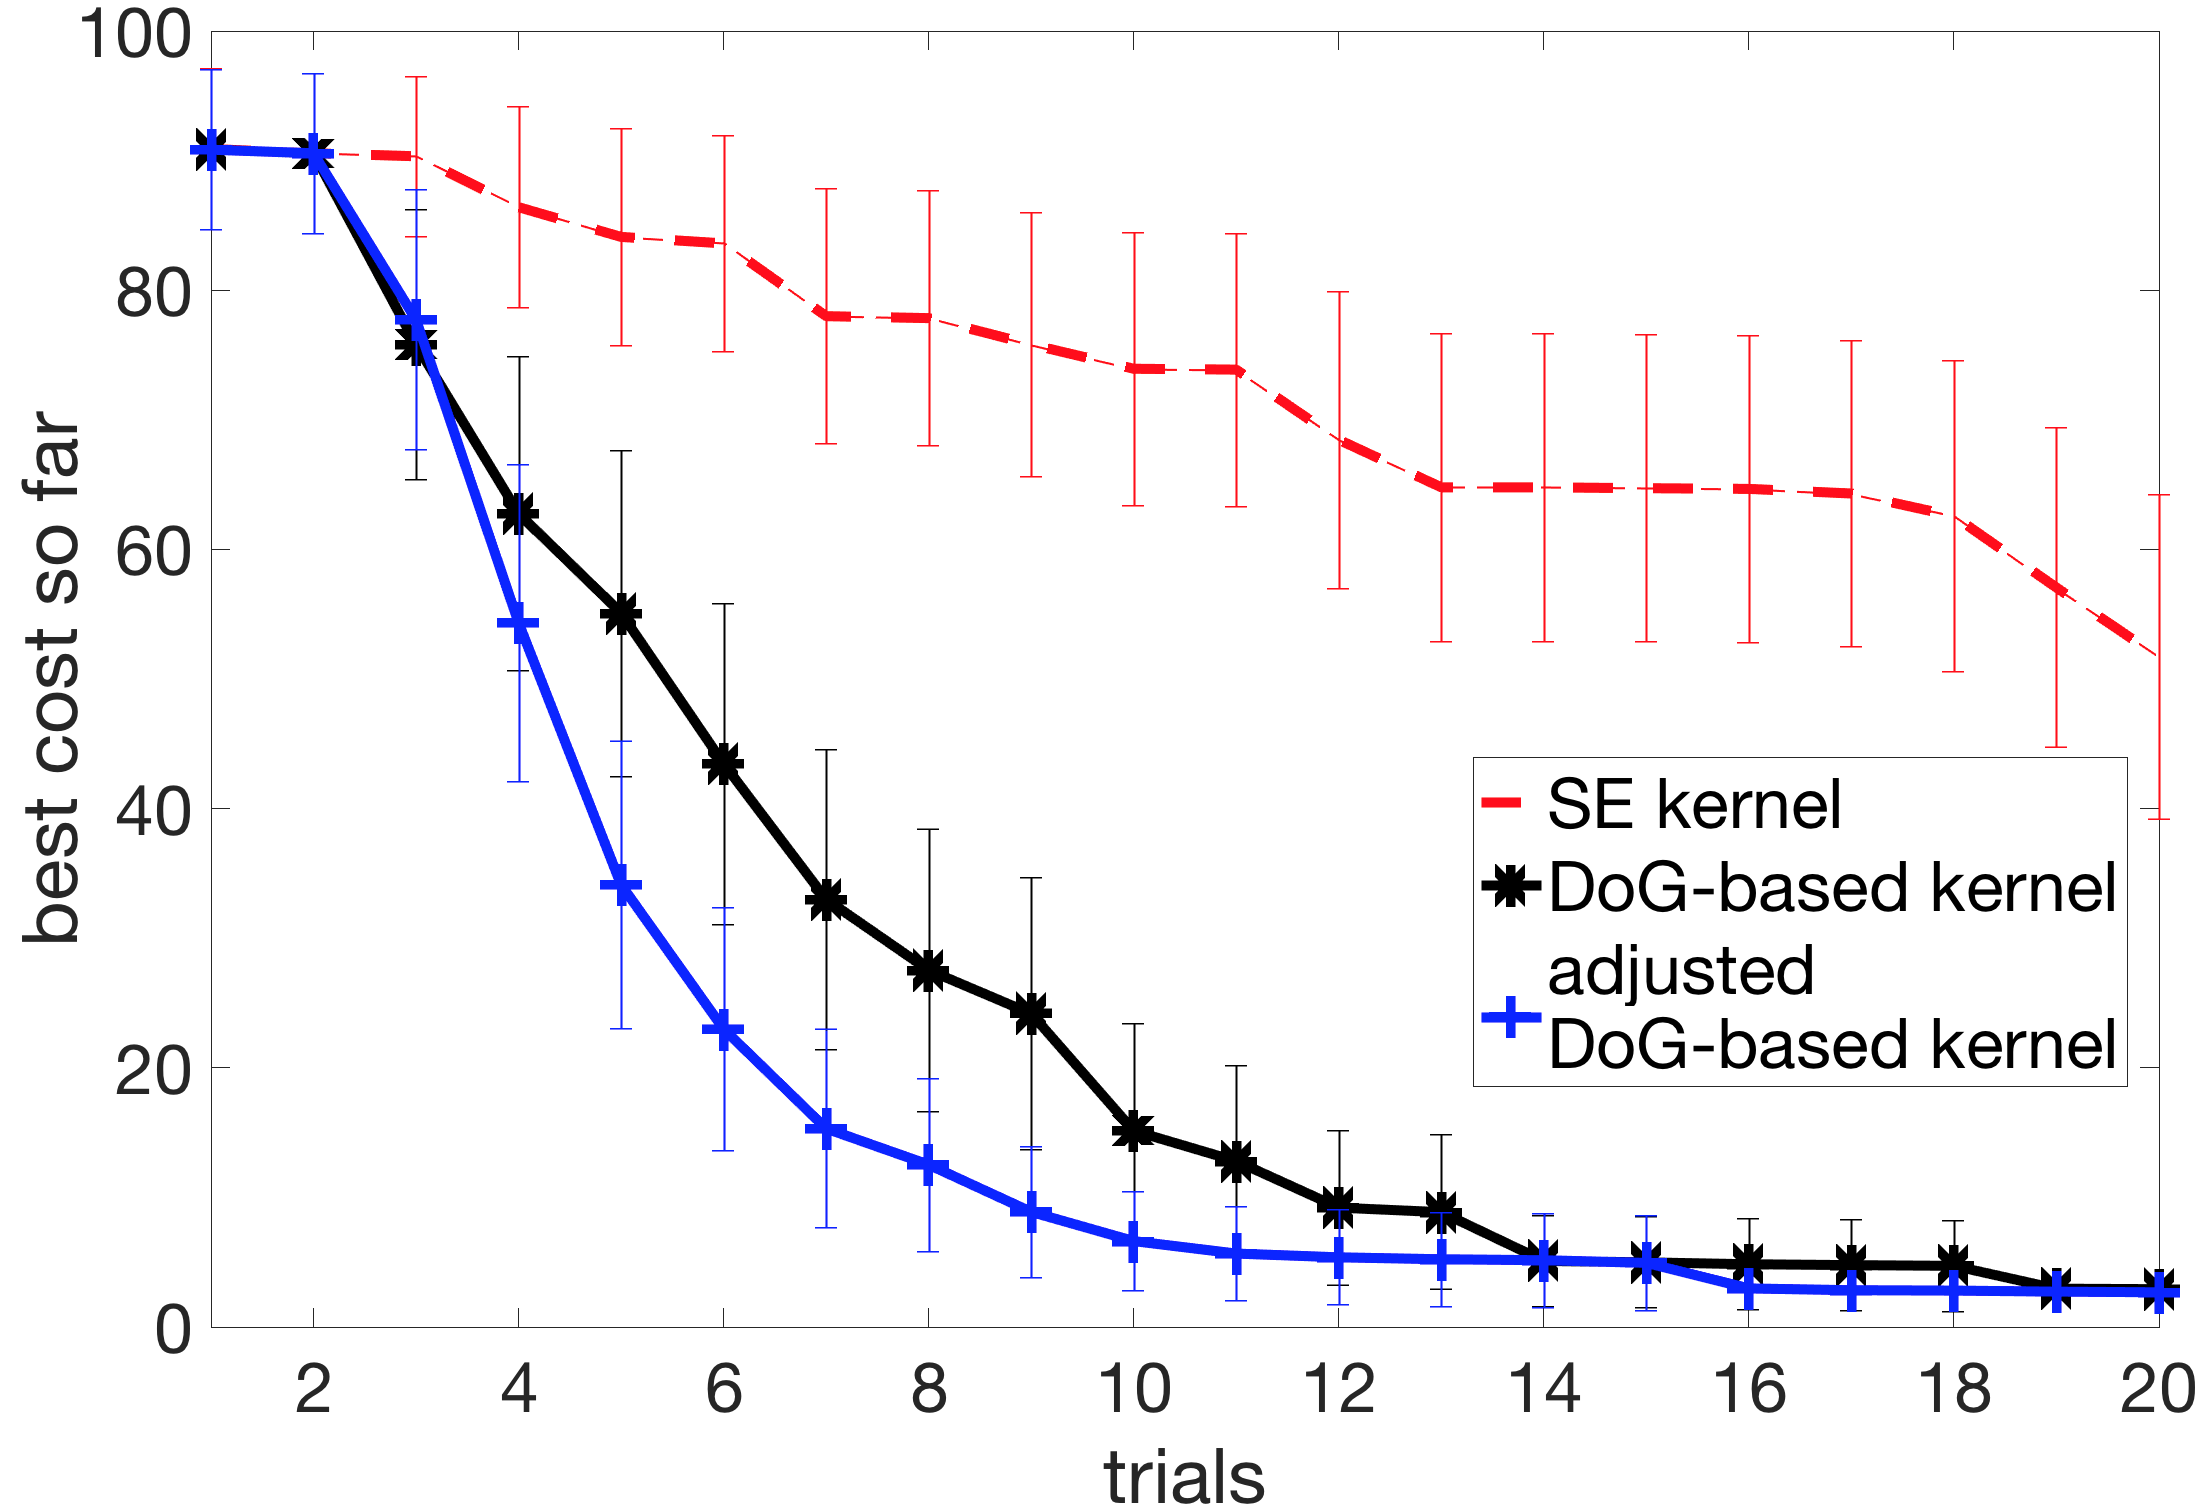
\includegraphics[width=0.5\textwidth]{img/sim_NM_Atrias_50d.png}
%\caption{\small{BO for 50d controller on original ATRIAS simulation.}}
%\label{fig:50d_sim}
%\end{figure}

In this section, we describe our experiments with increasing simulation-hardware mismatch and its effect on approaches that use information from simulation during hardware optimization. The quality of information transfer between simulation and hardware depends not only on the mismatch between the two, but also on the controller used. For a robust controller, small dynamics errors would not cause a significant deterioration in performance, while for a sensitive controller this might be much more detrimental. There is still an advantage to studying such a sensitive controller, as it might be much more energy efficient and versatile. In our experiments, the 50-dimensional VNMC described in Section \ref{subsec:VNMC_cont} is capable of generating very efficient gaits but is sensitive to modelling errors. Figure \ref{fig:sim_NM_Atrias_50d} shows the performance of the DoG-based and adjusted DoG-based kernel on the original high-fidelity simulator. While both methods find walking points in 20 trials, adjusted-DoG performs better. There is mismatch even between short $5s$ and long $30s$ simulations for this controller. This mismatch is compensated by the adjusted-DoG kernel.


In the rest of this section, we provide experimental analysis of settings with increasing simulated mismatch and their effect on optimization of the 50-dimensional VNMC. We compare several approaches that improve sample-efficiency of BO and investigate if the improvement they offer is robust to mismatch between the simulated setting used for constructing kernel/prior and the setting on which BO is run. 

\subsection{Incorrect dynamics models}
\begin{figure}[t]
\begin{subfigure}[t]{0.47\textwidth}
\centering
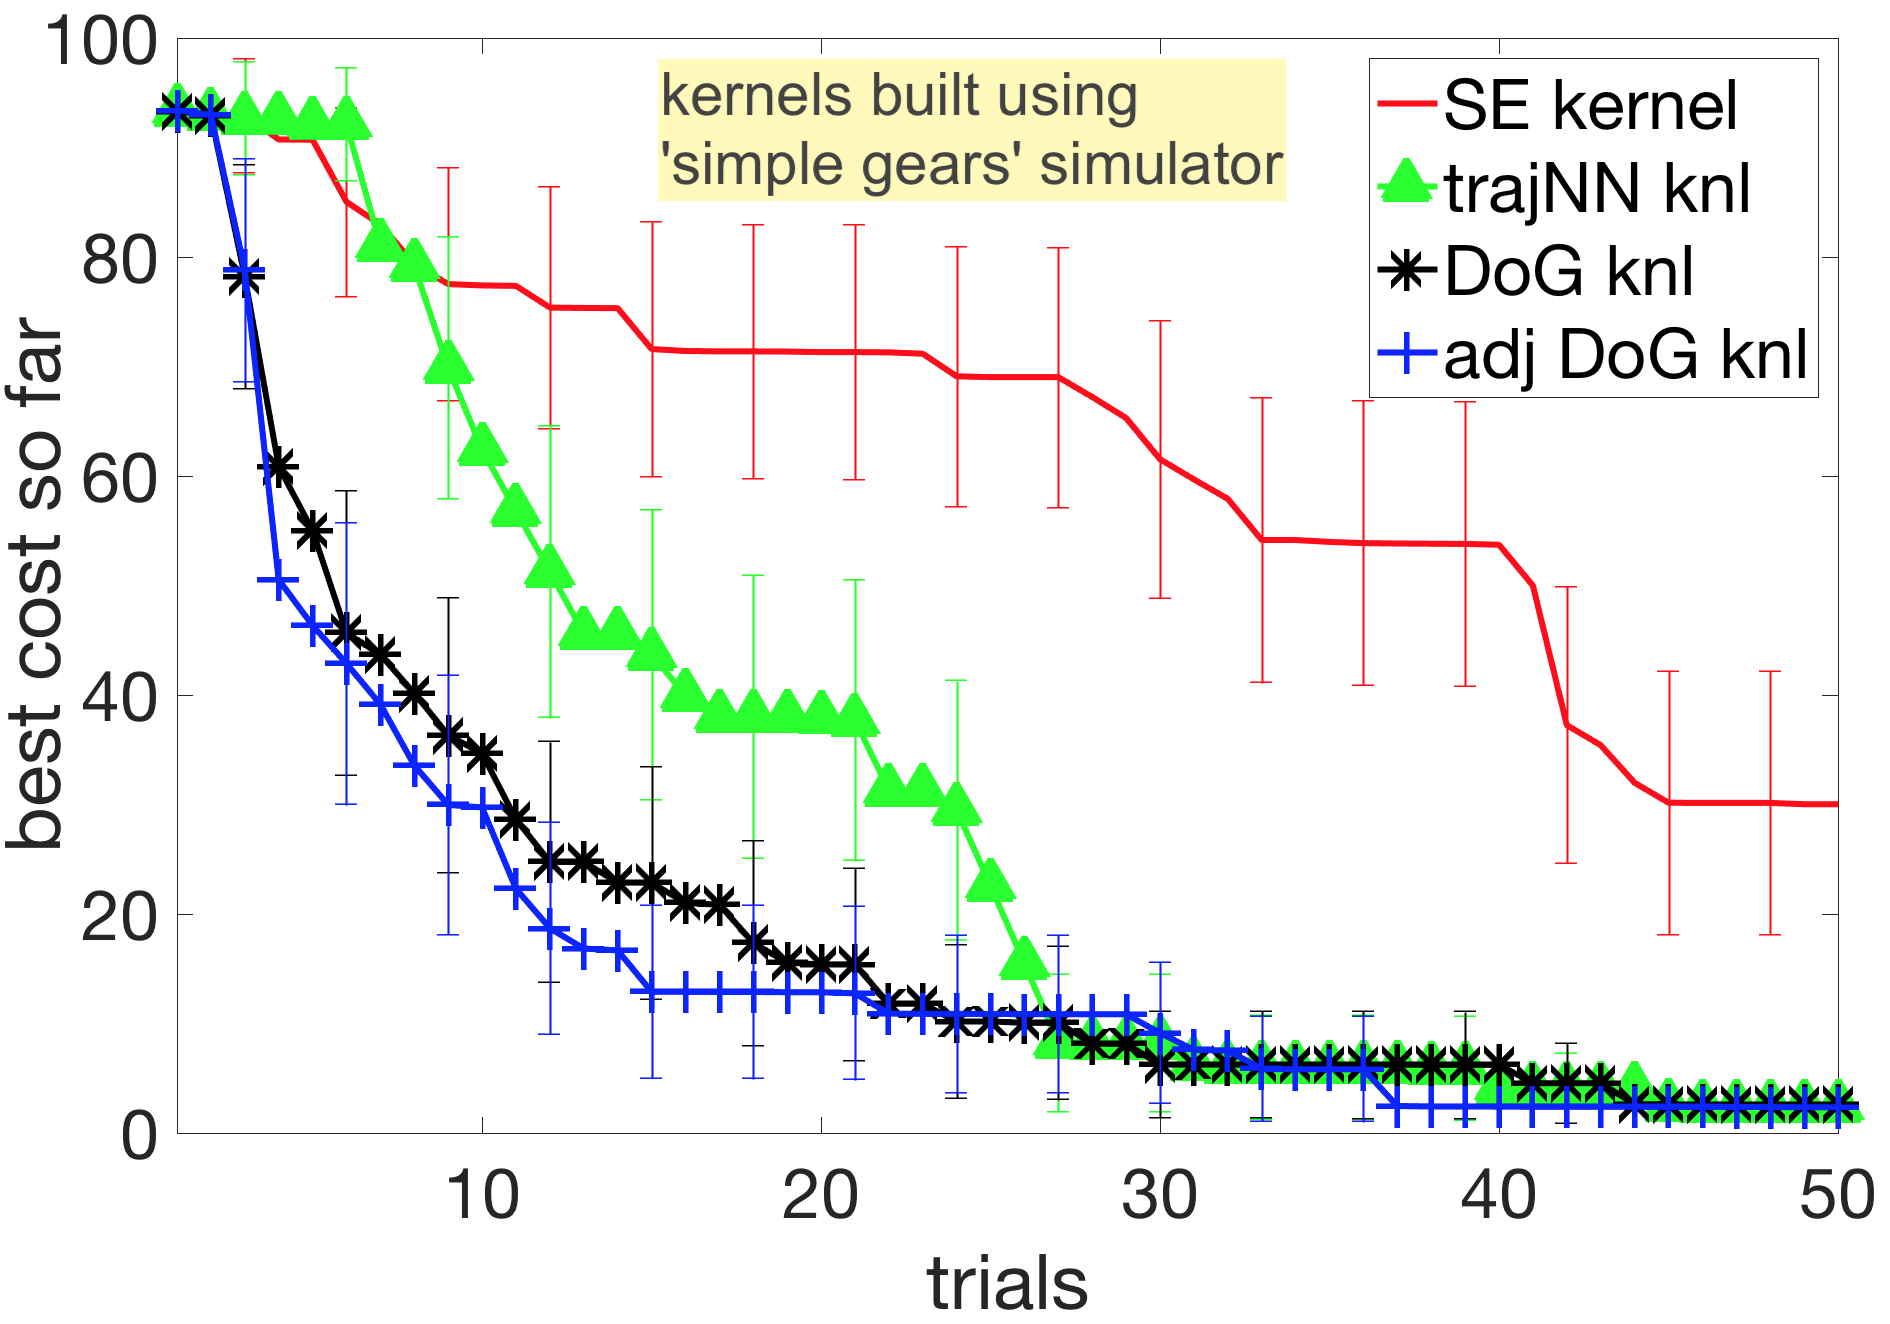
\includegraphics[width=1.0\textwidth]{img/compare_gear_dynamics.png}
\caption{\small{Informed kernels generated using simulator with simplified gear dynamics.}}
\label{fig:compare_gear_dynamics}
\end{subfigure}
\hspace{10px}
\begin{subfigure}[t]{0.47\textwidth}
\centering
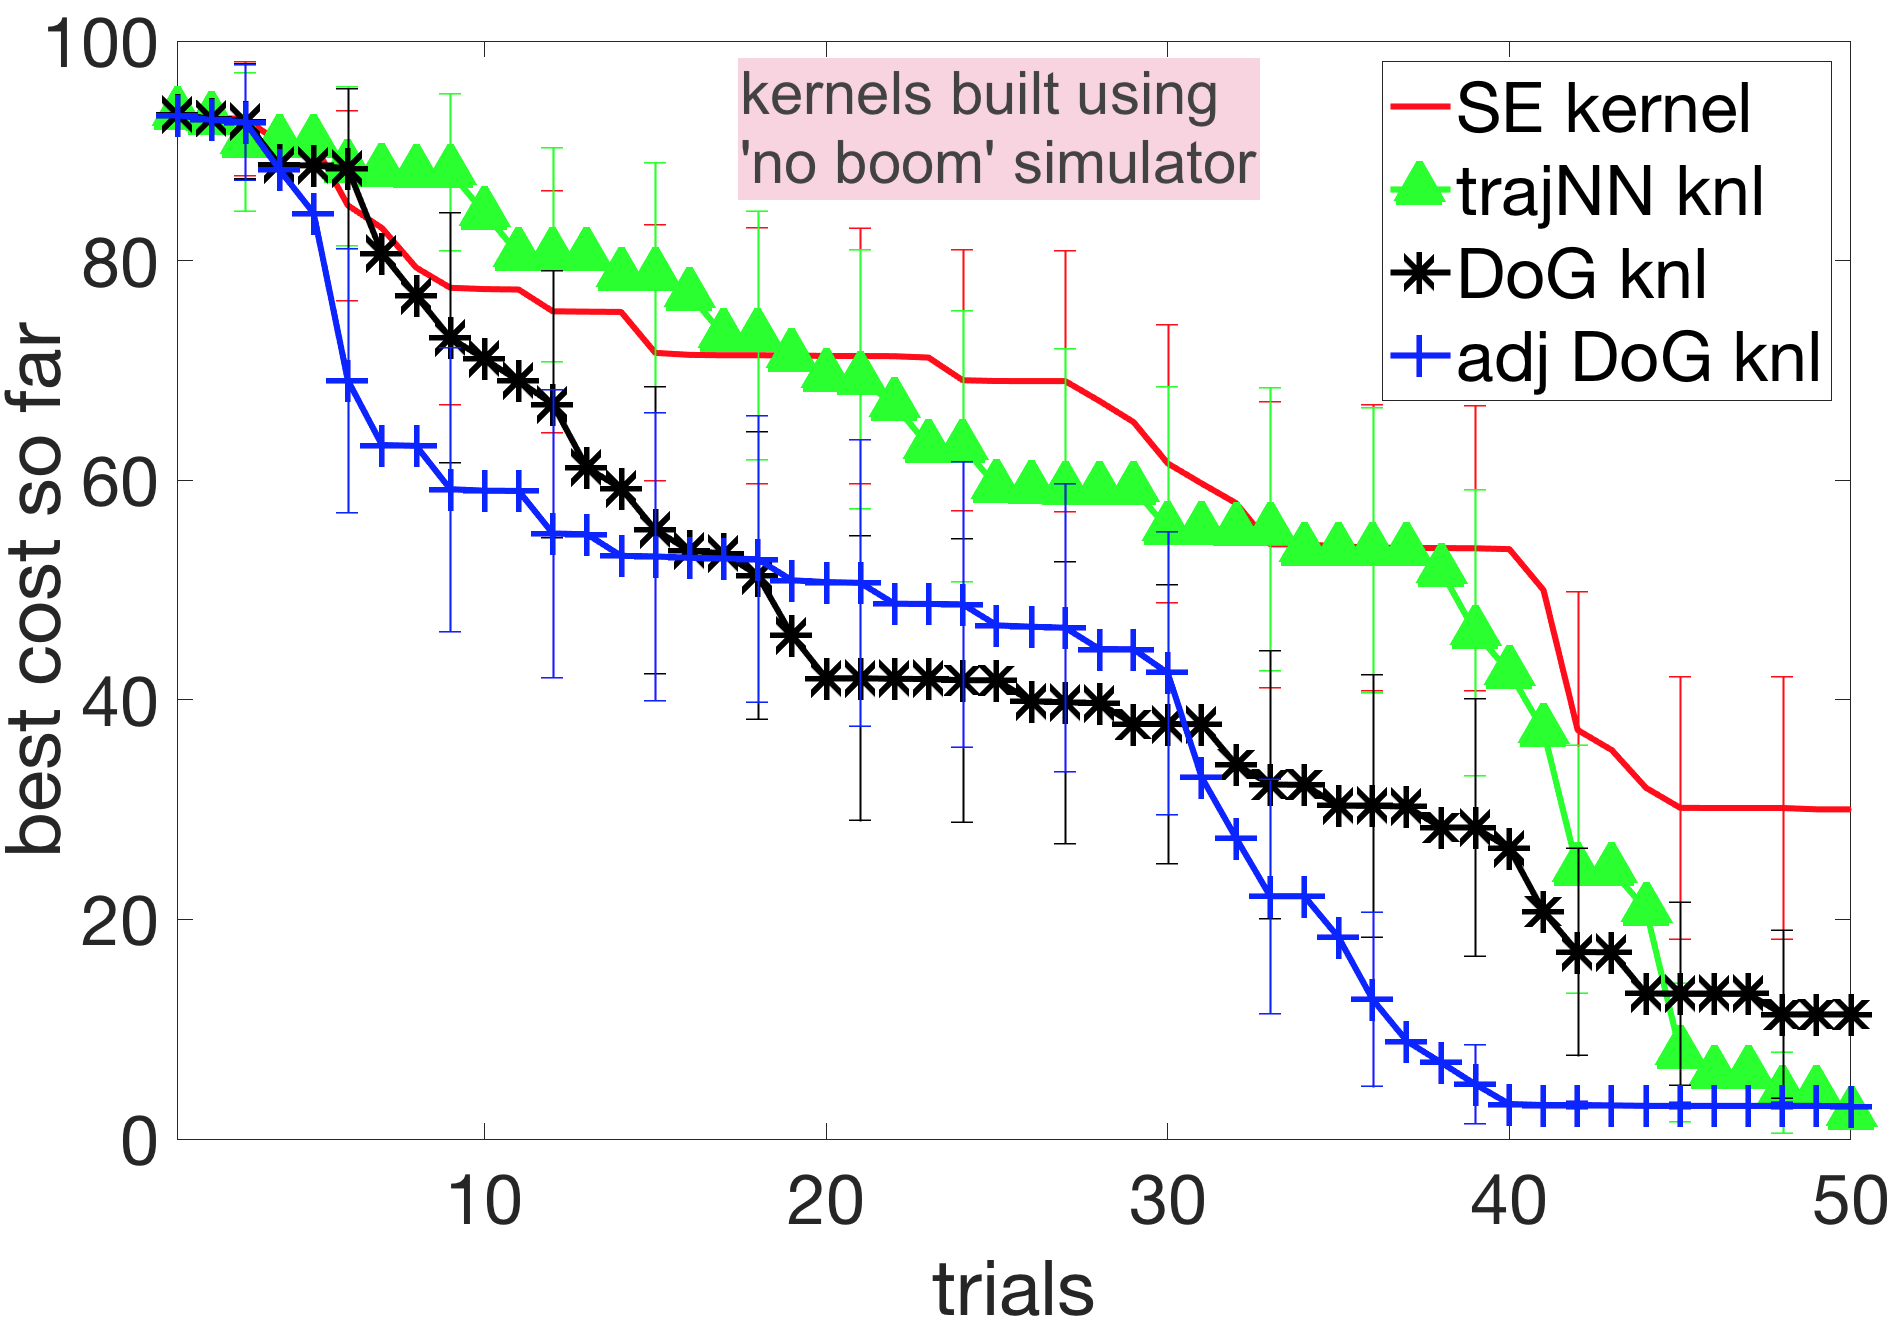
\includegraphics[width=1.0\textwidth]{img/compare_without_boom.png}
\caption{\small{Informed kernels generated using simplified gear dynamics, without boom model.}}
\label{fig:compare_without_boom}
\end{subfigure}
\caption{\small{BO is run on the original simulator. Informed kernels perform well despite significant mismatch, when kernels are generated using simulator with simplified gear dynamics (left). In the case of severe mismatch, when the boom model is also removed, informed kernels still improve over baseline SE (right). Plots show best cost for mean over 50 runs for each algorithm, 95\% CIs.}}
\label{fig:compare_dog}
\end{figure} 
First, we examine the performance of our proposed approaches with informed kernels: $k_{DoG}$, $k_{\text{trajNN}}$ and $k_{DoG_{adj}}$. Figure~\ref{fig:compare_gear_dynamics} shows the case when informed kernels are generated using inaccurate dynamics models, as described in Section \ref{}. The first approximate simulator has simplified gear dynamics while BO is run on the original simulator. The second approximation removes the boom of the robot and simulates a purely 2-dimensional robot.

When kernel is generated in simulator with approximate gear dynamics, all runs with informed kernels find walking solutions in 50 trials, while for SE only $70\%$ of the runs have walking solutions.

Next, Figure~\ref{fig:compare_without_boom} shows performance of $k_{DoG}$, $k_{\text{trajNN}}$ and $k_{DoG_{adj}}$ when the kernels are constructed using a simulator with simplified dynamics and without a the boom. In this case the mismatch with the original simulator is larger than before and we see the advantage of using adjustment for DoG-based kernel: $k_{DoG_{adj}}$ finds walking points in all runs after 35 trials. $k_{\text{trajNN}}$ also achieves this, but after 50 trials. $k_{DoG}$ finds walking points in $\approx\!90\%$ of the runs after 50 trials. The performance of SE stays the same, as it uses no prior information from any simulator.

This illustrates that while the original DoG-based kernel can recover from slight simulation-hardware mismatch, the adjusted DoG-kernel is required if one expects higher mismatch.  $k_{\text{trajNN}}$ seems to recover from the mismatch, but might benefit from an adjusted version. We leave this to future work.

%------------------------------------------------------------------------------------
\subsubsection{Comparisons of Prior-based and Kernel-based Approaches}
\label{subsec:sim_experiments_prior_cully}
We will classify approaches that use simulation information in hardware optimization as prior-based or kernel-based. Prior-based approaches use costs from the simulation in the prior of the GP used in the BO. This can help BO a lot if the costs between simulation and hardware transfer, and the cost function is fixed. However, in the presence of large mismatch, points that perform well in simulation might fail on hardware. A prior-based method can be biased towards sampling promising points from simulation, resulting in an even poorer performance than methods with no prior. Kernel-based approaches consist of methods that incorporate the information from simulation into the kernel of the GP. These can be sample-inefficient as compared to prior-based method, but less likely to be biased towards unpromising regions in the presence of mismatch. They also easily generalize to multiple costs, so that there is no additional computation if the cost is changed. This is important because a lot of these approaches can take several days of computation to generate the informed kernel. For example, \cite{cully2015robots} report taking 2 weeks on a 16-core computer to generate their map. 
\begin{figure}[t]
\begin{subfigure}[t]{0.47\textwidth}
\centering
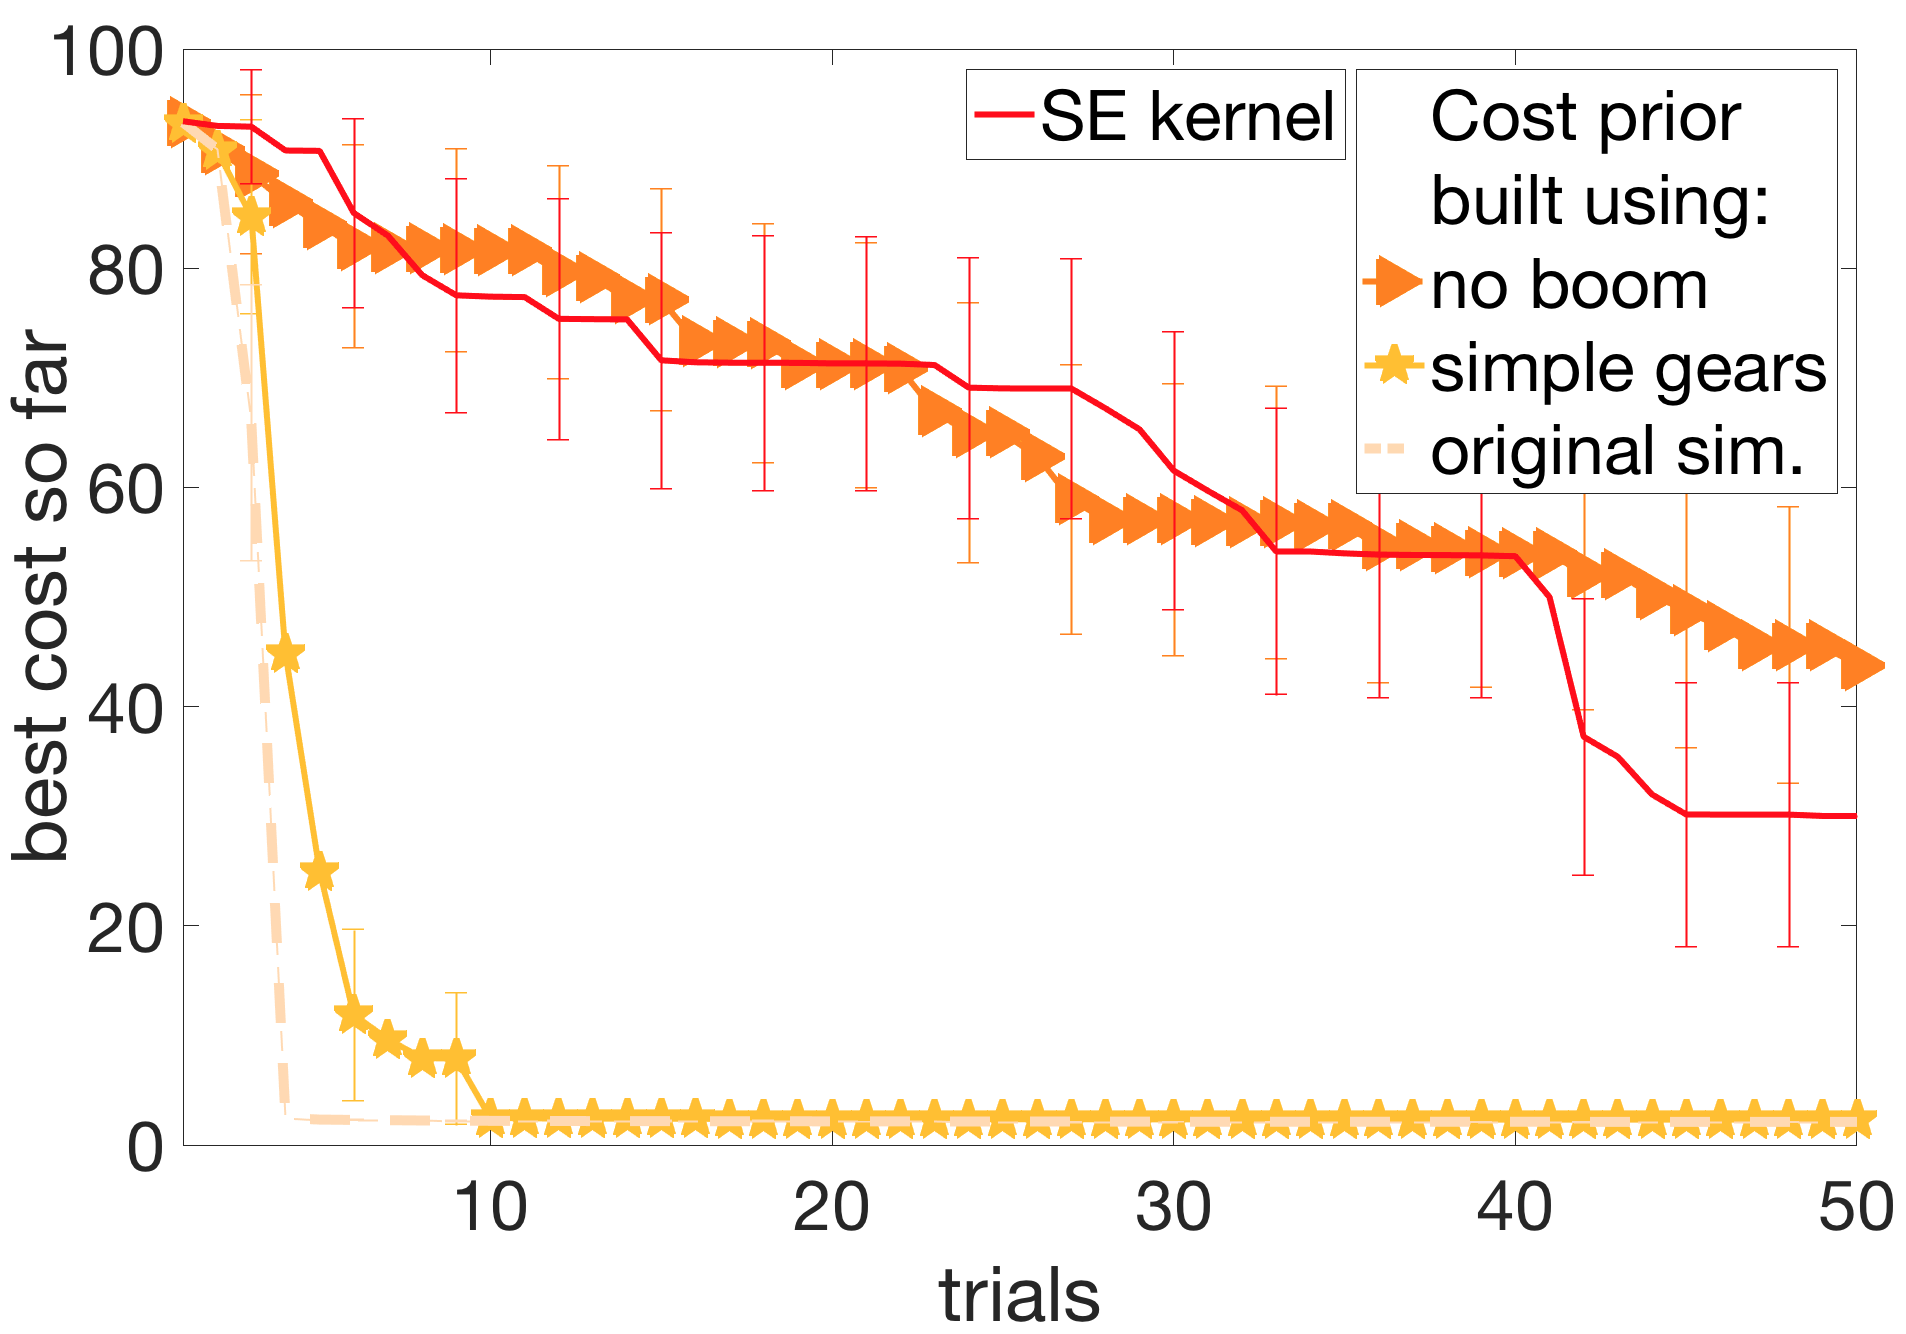
\includegraphics[width=1.0\textwidth]{img/cost_prior_sim_versions.png}
\caption{\small{BO with cost prior: straightforward approach useful for low-to-medium mismatch; but no improvement if mismatch is severe.}}
\label{fig:cost_prior_sim_versions}
\end{subfigure}
\hspace{15px}
\begin{subfigure}[t]{0.47\textwidth}
\centering
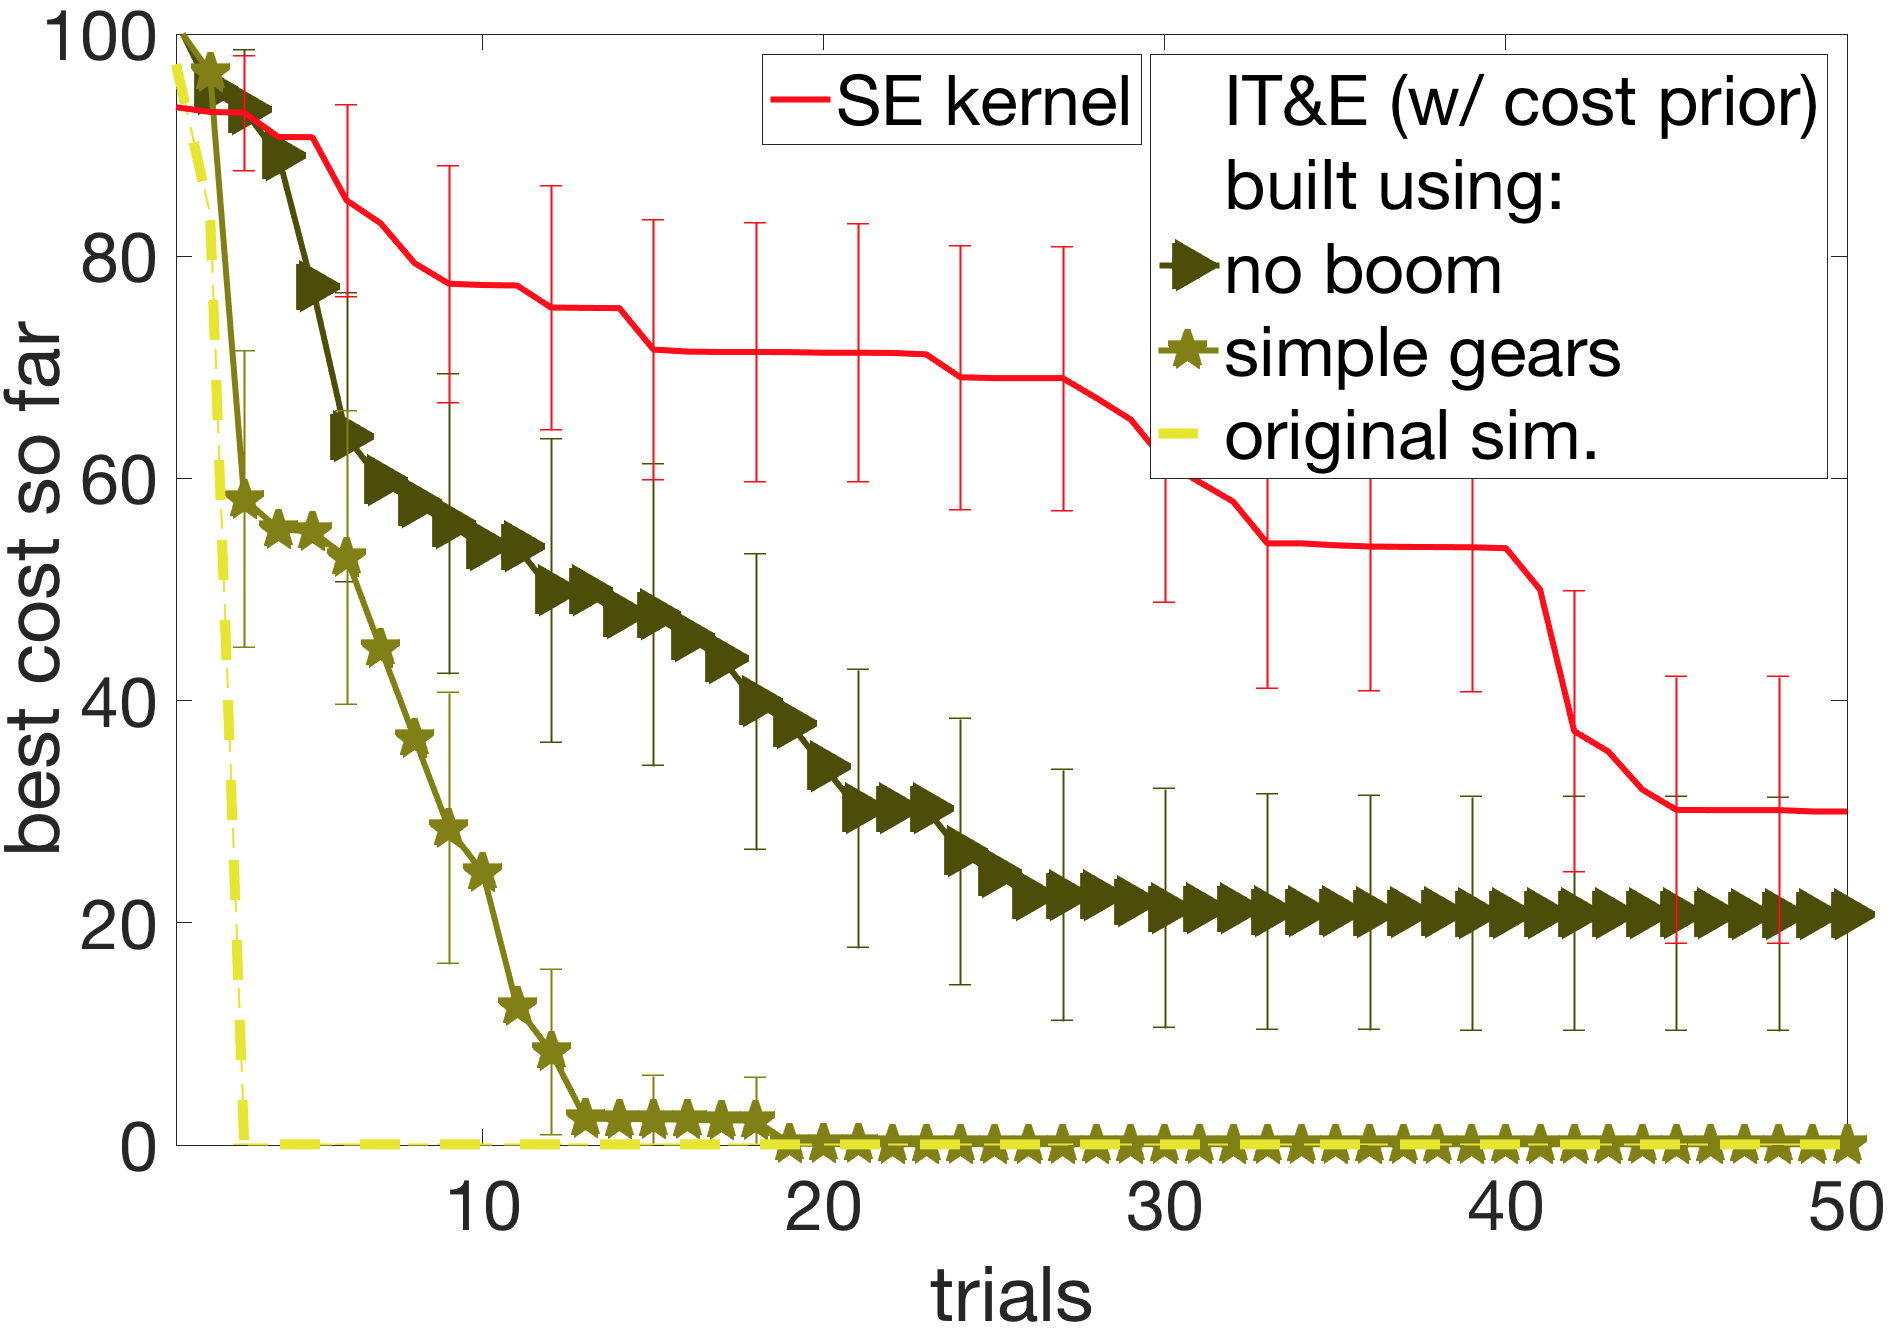
\includegraphics[width=1.0\textwidth]{img/cully_prior_sim_versions.png}
\caption{\small{Performance of IT\&E algorithm (our implementation of \citet{cully2015robots}, adapted to bipedal locomotion).}}
\label{fig:cully_prior_sim_versions}
\end{subfigure}
\caption{\small{BO using prior-based approaches. Mean over 50 runs for each algorithm, 95\% CIs.}}
\label{fig:prior_based_bo}
\end{figure}

It is possible to also combine both prior-based and kernel-based methods, as in \cite{cully2015robots}. We will classify these as `prior-based' methods, since in our experiments prior outweighs the kernel effects for such cases. In our comparison with \cite{cully2015robots}, we will implement a version with and without the prior points. We do not add a cost prior to BO using DoG-based kernel, as this limits us to a particular cost, and high-fidelity simulators. Since both of these can be major obstacles in real robot experiments, we refrain from doing so.


Figure~\ref{fig:cost_prior_sim_versions} shows the performance when using simulation cost in the prior during BO, and learning a model for the difference between simulation and hardware costs \citep{wilson2014using}. BO with a cost prior created using the original version of the simulator illustrates what would happen in the best case scenario, as optimization is merely a look-up here. When the simulator with simplified gear dynamics is used for constructing the prior, we observe significant improvements over uninformed BO prior. However, when the prior is constructed from simplified gear dynamics and no boom setting, the approach performs slightly worse than uninformed BO. This shows that while an informed prior can be very helpful when created from a simulator close to hardware, it can hurt performance if simulator is significantly different from hardware. 


\begin{figure}[t]
\begin{subfigure}[t]{0.47\textwidth}
\centering
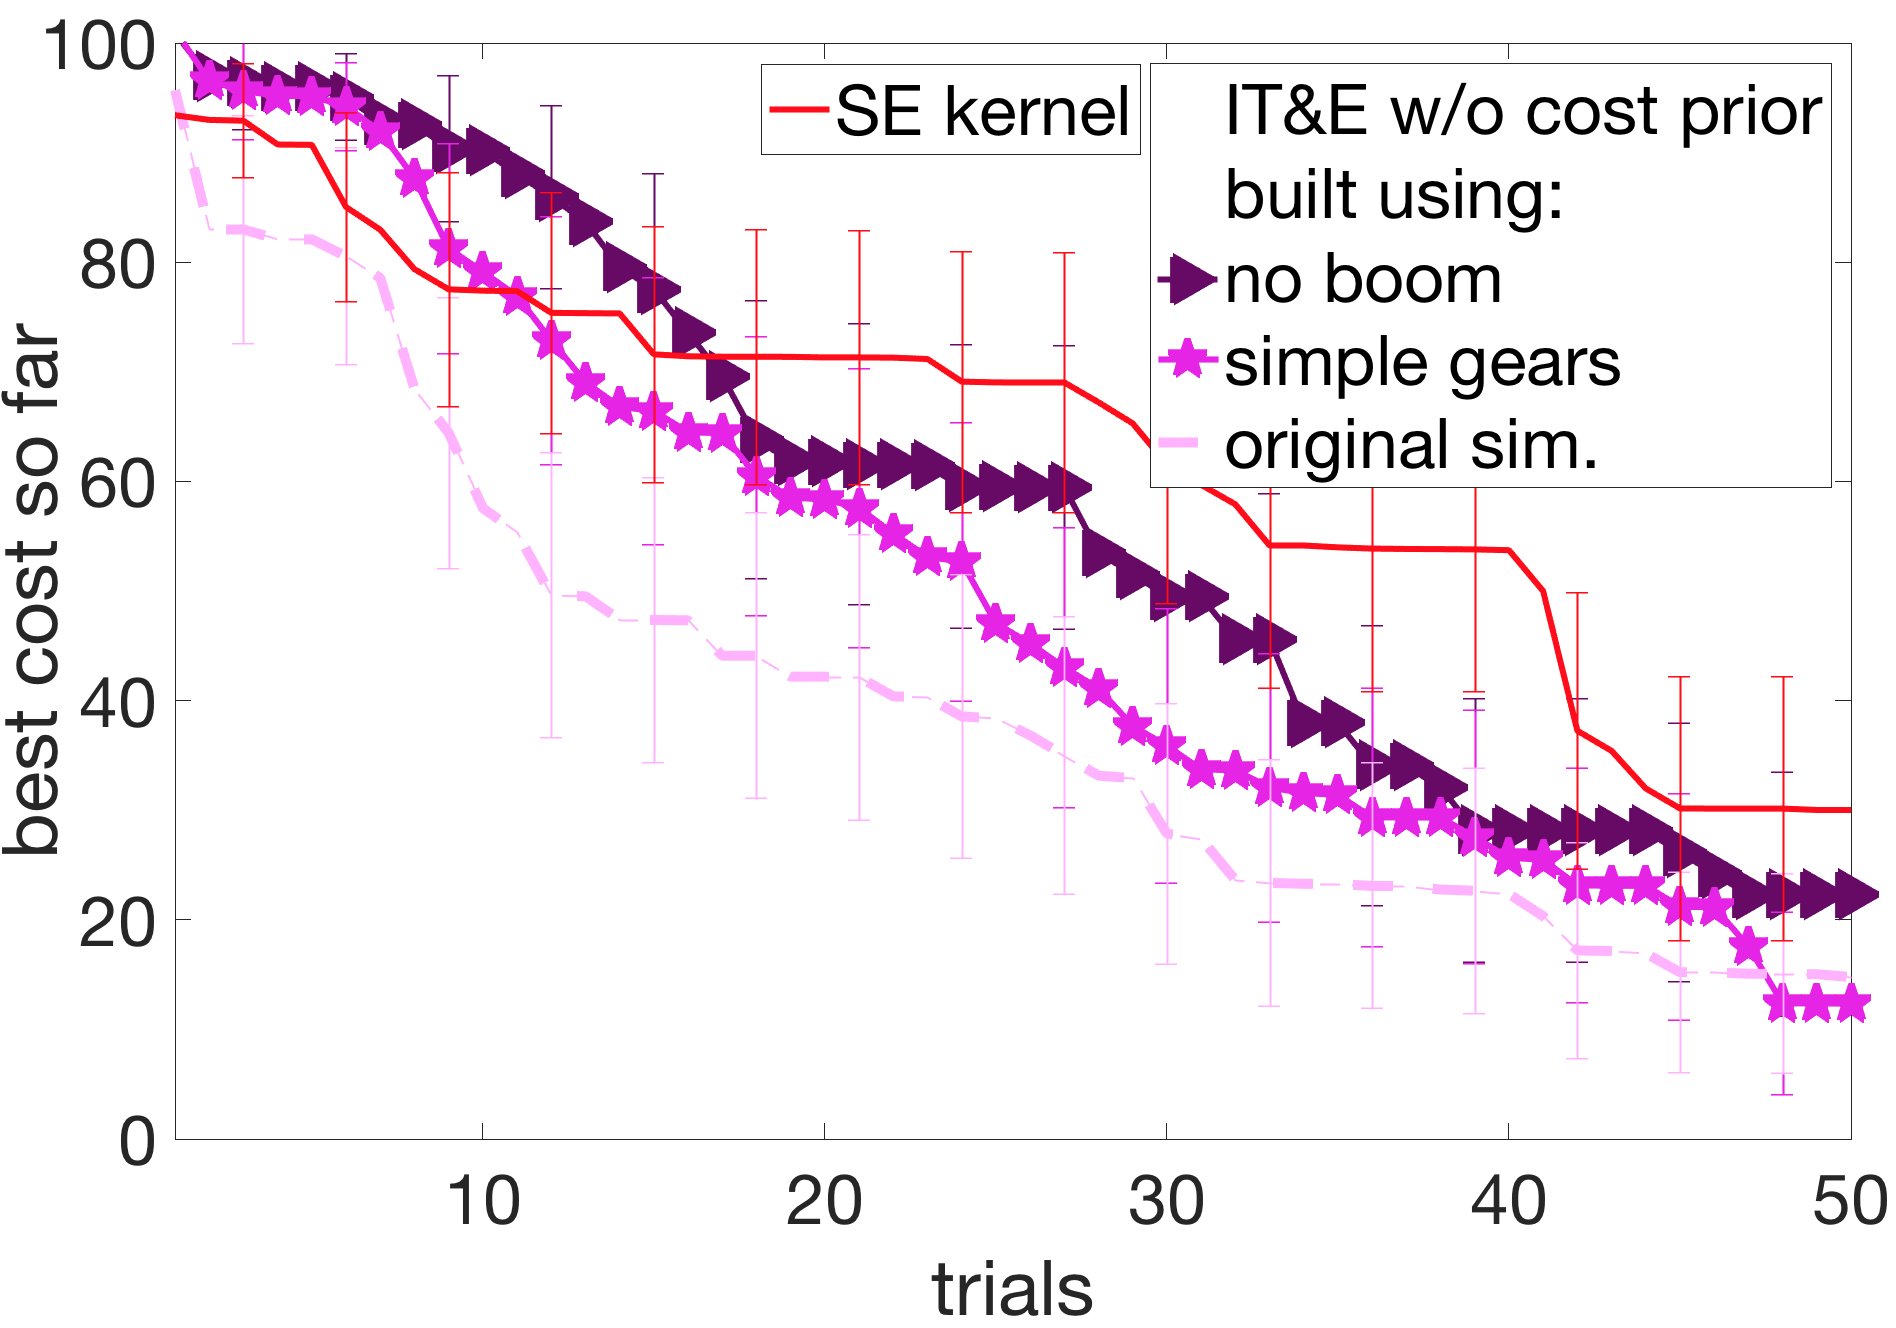
\includegraphics[width=1.0\textwidth]{img/cully_no_prior_sim_versions.png}
\caption{\small{BO using our implementation of IT\&E without cost prior (from \citet{cully2015robots}).}}
\label{fig:cully_kernel_sim_versions}
\end{subfigure}
\hspace{10px}
\begin{subfigure}[t]{0.47\textwidth}
\centering
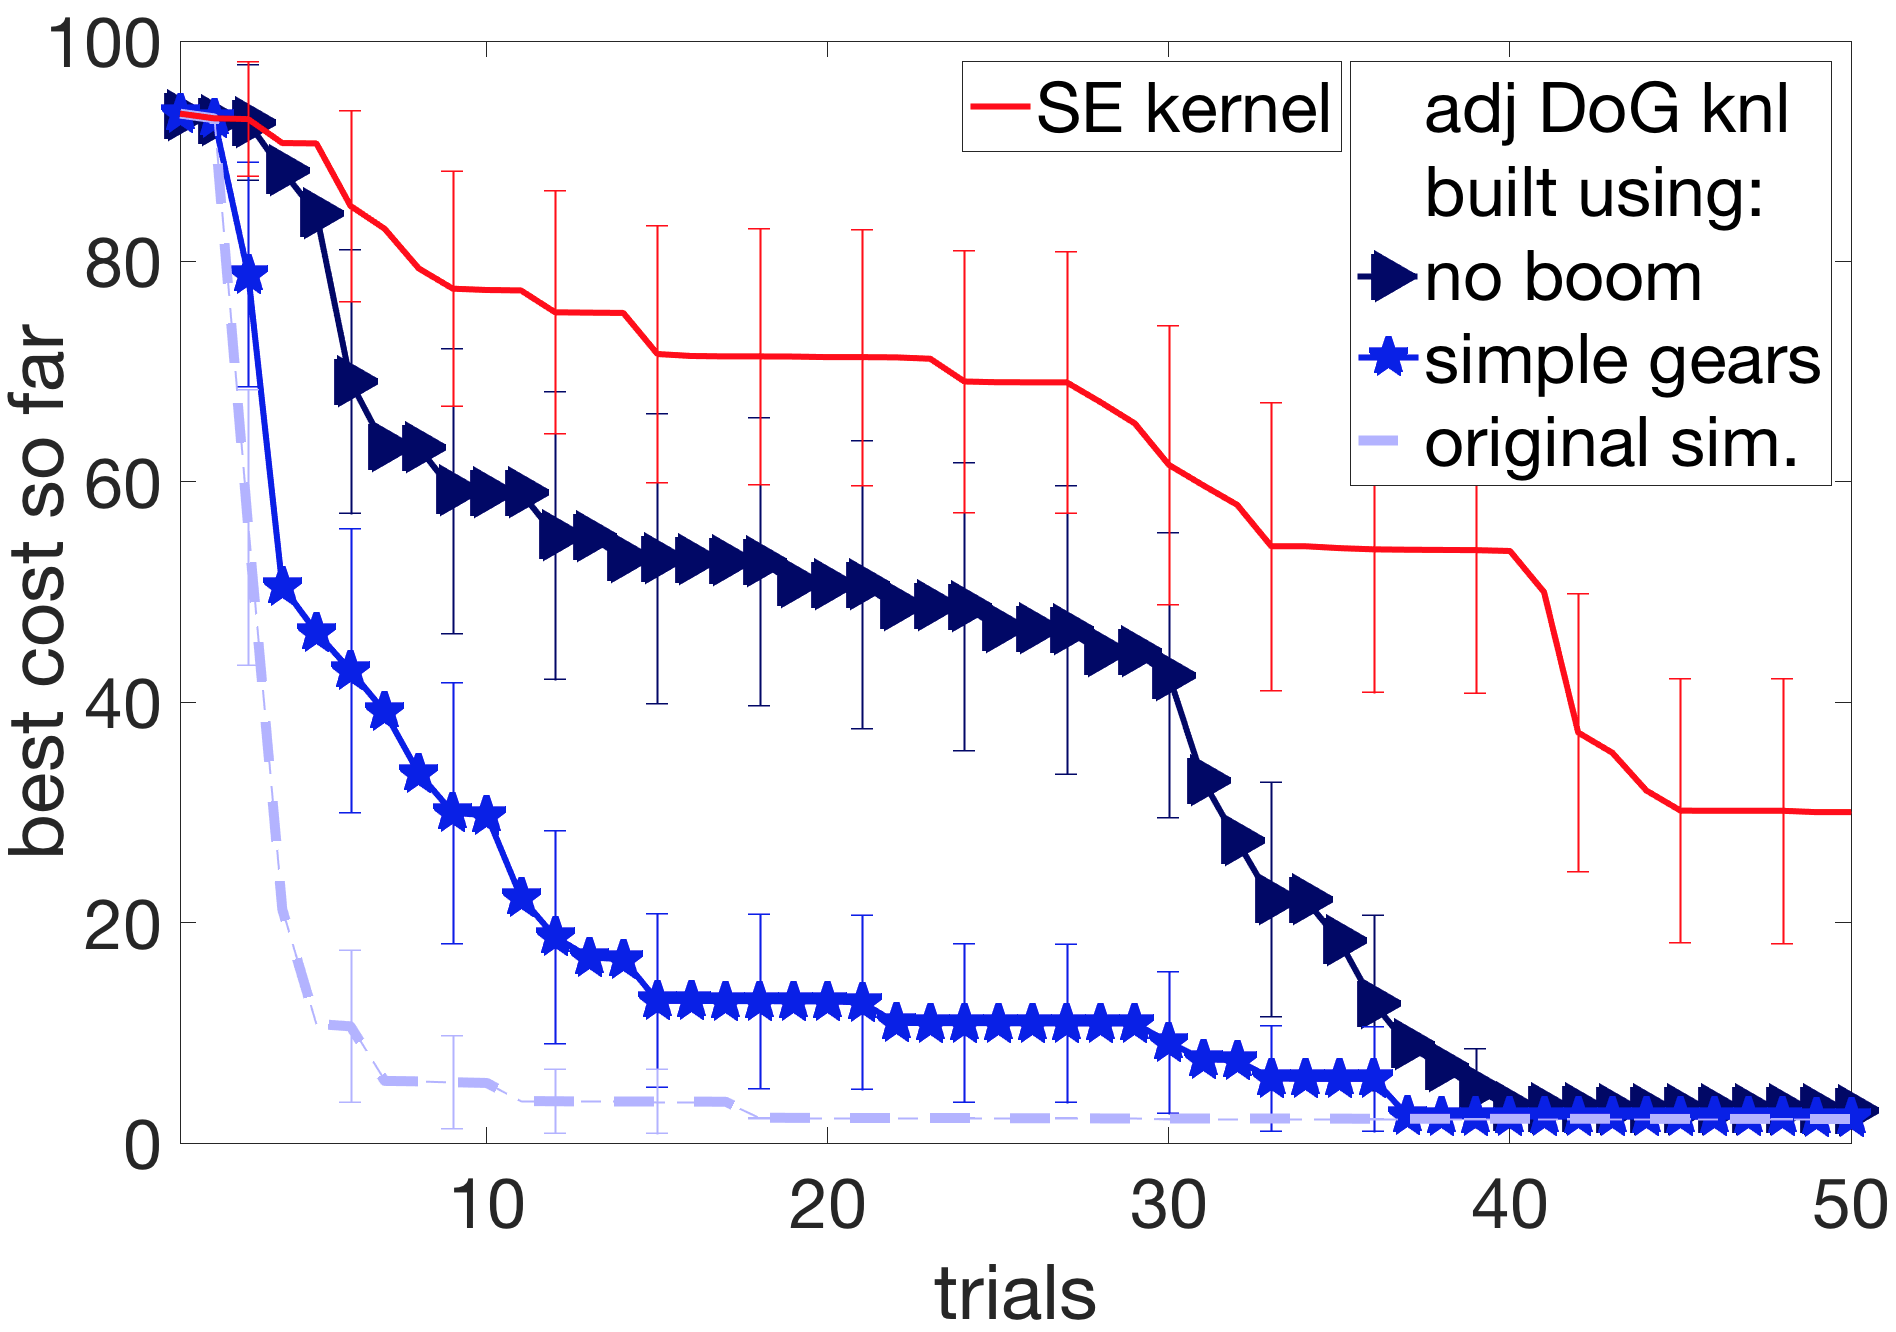
\includegraphics[width=1.0\textwidth]{img/dog_hwadjust1_sim_versions.png}
\caption{\small{BO using $k_{DoG_{adj}}$ constructed from simulators with various levels of mismatch.}}
\label{fig:kernel_hwadjust2_sim_versions}
\end{subfigure}
\caption{\small{BO using kernel-based approaches. Mean over 50 runs for each algorithm, 95\% CIs.}}
\label{fig:prior_based_bo}
\end{figure}


Next, we discuss experiments with our implementation of Intelligent Trial and Error (IT\&E) algorithm from~\citet{cully2015robots}. This algorithm combines adding a cost prior from simulated evaluations with adding simulation information into the kernel. IT\&E defines a behavior metric and tabulates best performing points from simulation on their corresponding behavior score. The behavior metric used in our experiments is duty-factor of each leg, which can go from 0 to 1.0. We discretize the duty factor into 21 cells of 0.05 increments, leading to a $21\times21$ grid. We collect the 5 highest performing controllers for each square in the behavior grid, creating a $21\times21\times5$ grid. Next, we generate 50 random combinations of a $21\times21$ grid, selecting 1 out of the 5 best controllers per grid cell. Care was taken to ensure that all 5 controllers had comparable costs in the simulator used for creating the map. 
Cost of each selected controller is added to the prior and BO was performed in the behavior space, like in \cite{cully2015robots}.

Figure~\ref{fig:cully_prior_sim_versions} shows BO with IT\&E constructed using different versions of the simulator. \mbox{IT\&E} constructed using simplified gear dynamics simulator is slightly less sample-efficient than the straightforward `cost prior' approach. When constructed with the simulator with no boom, \mbox{IT\&E} is able to improve over uninformed BO. However, it only finds walking points in 77\% of the runs in 50 trials in  this case, as some of the generated maps contained no controllers that could walk on the `hardware'. This is a shortcoming of the IT\&E algorithm, as it eliminates a very large part of the search space and if the pre-selected space does not contain a walking point, no walking controllers can be sampled with BO. This problem could possibly be avoided by using a finer grid, or a different behavior metric. However tuning such hyper-parameters can turn out to be expensive, in computation and hardware experiment time.



To separate the effects of using simulation information in prior mean vs kernel, we evaluated a kernel-only version of \mbox{IT\&E} algorithm. Figure~\ref{fig:cully_kernel_sim_versions} shows these results. It shows that the cost prior is crucial for the success of IT\&E and performance deteriorates without it. Hence, it is not practical to use IT\&E on a cost different than what it was generated for.

Nonetheless, Figure~\ref{fig:compare_dog} showed that BO with adjusted DoG kernel is able to handle both moderate and severe mismatch with kernel-only information, collected in  Figure~\ref{fig:kernel_hwadjust2_sim_versions}.

In summary, we created two simulators with increasing modelling approximations, and studied the effect of using these to aid optimization on the original simulator. We found that while methods that use cost in the prior of BO can be very sample-efficient in low mismatch, their performance worsens as mismatch increases. \mbox{IT\&E} introduced in \cite{cully2015robots} uses simulation information in both prior mean and kernel, and is very sample-efficient in cases of low mismatch. Even with high mismatch, it performs better than just prior-based BO but doesn't find walking controllers reliably. In comparison, adjusted DoG-based kernel performed well in all the tested scenarios. All of this shows that the adjusted DoG-based kernel can reliably improve sample-efficiency of BO even when the mismatch between simulation and hardware is high. We would like to continue working in this direction and explore the usefulness of even simpler simulators in the future.

\AR{Add note about smooth cost and performance}

\subsection{Incorrect dynamics parameters}

Our next set of experiments create ``simulated hardware" that is increasingly different from the simulation, in which the DoG features were collected. This is done by changing the mass, inertia, center of mass location, friction coefficient of the ground contact models, ground stiffness and actuator delay, as described in Section \ref{}.

\begin{figure}[h!]
\centering
    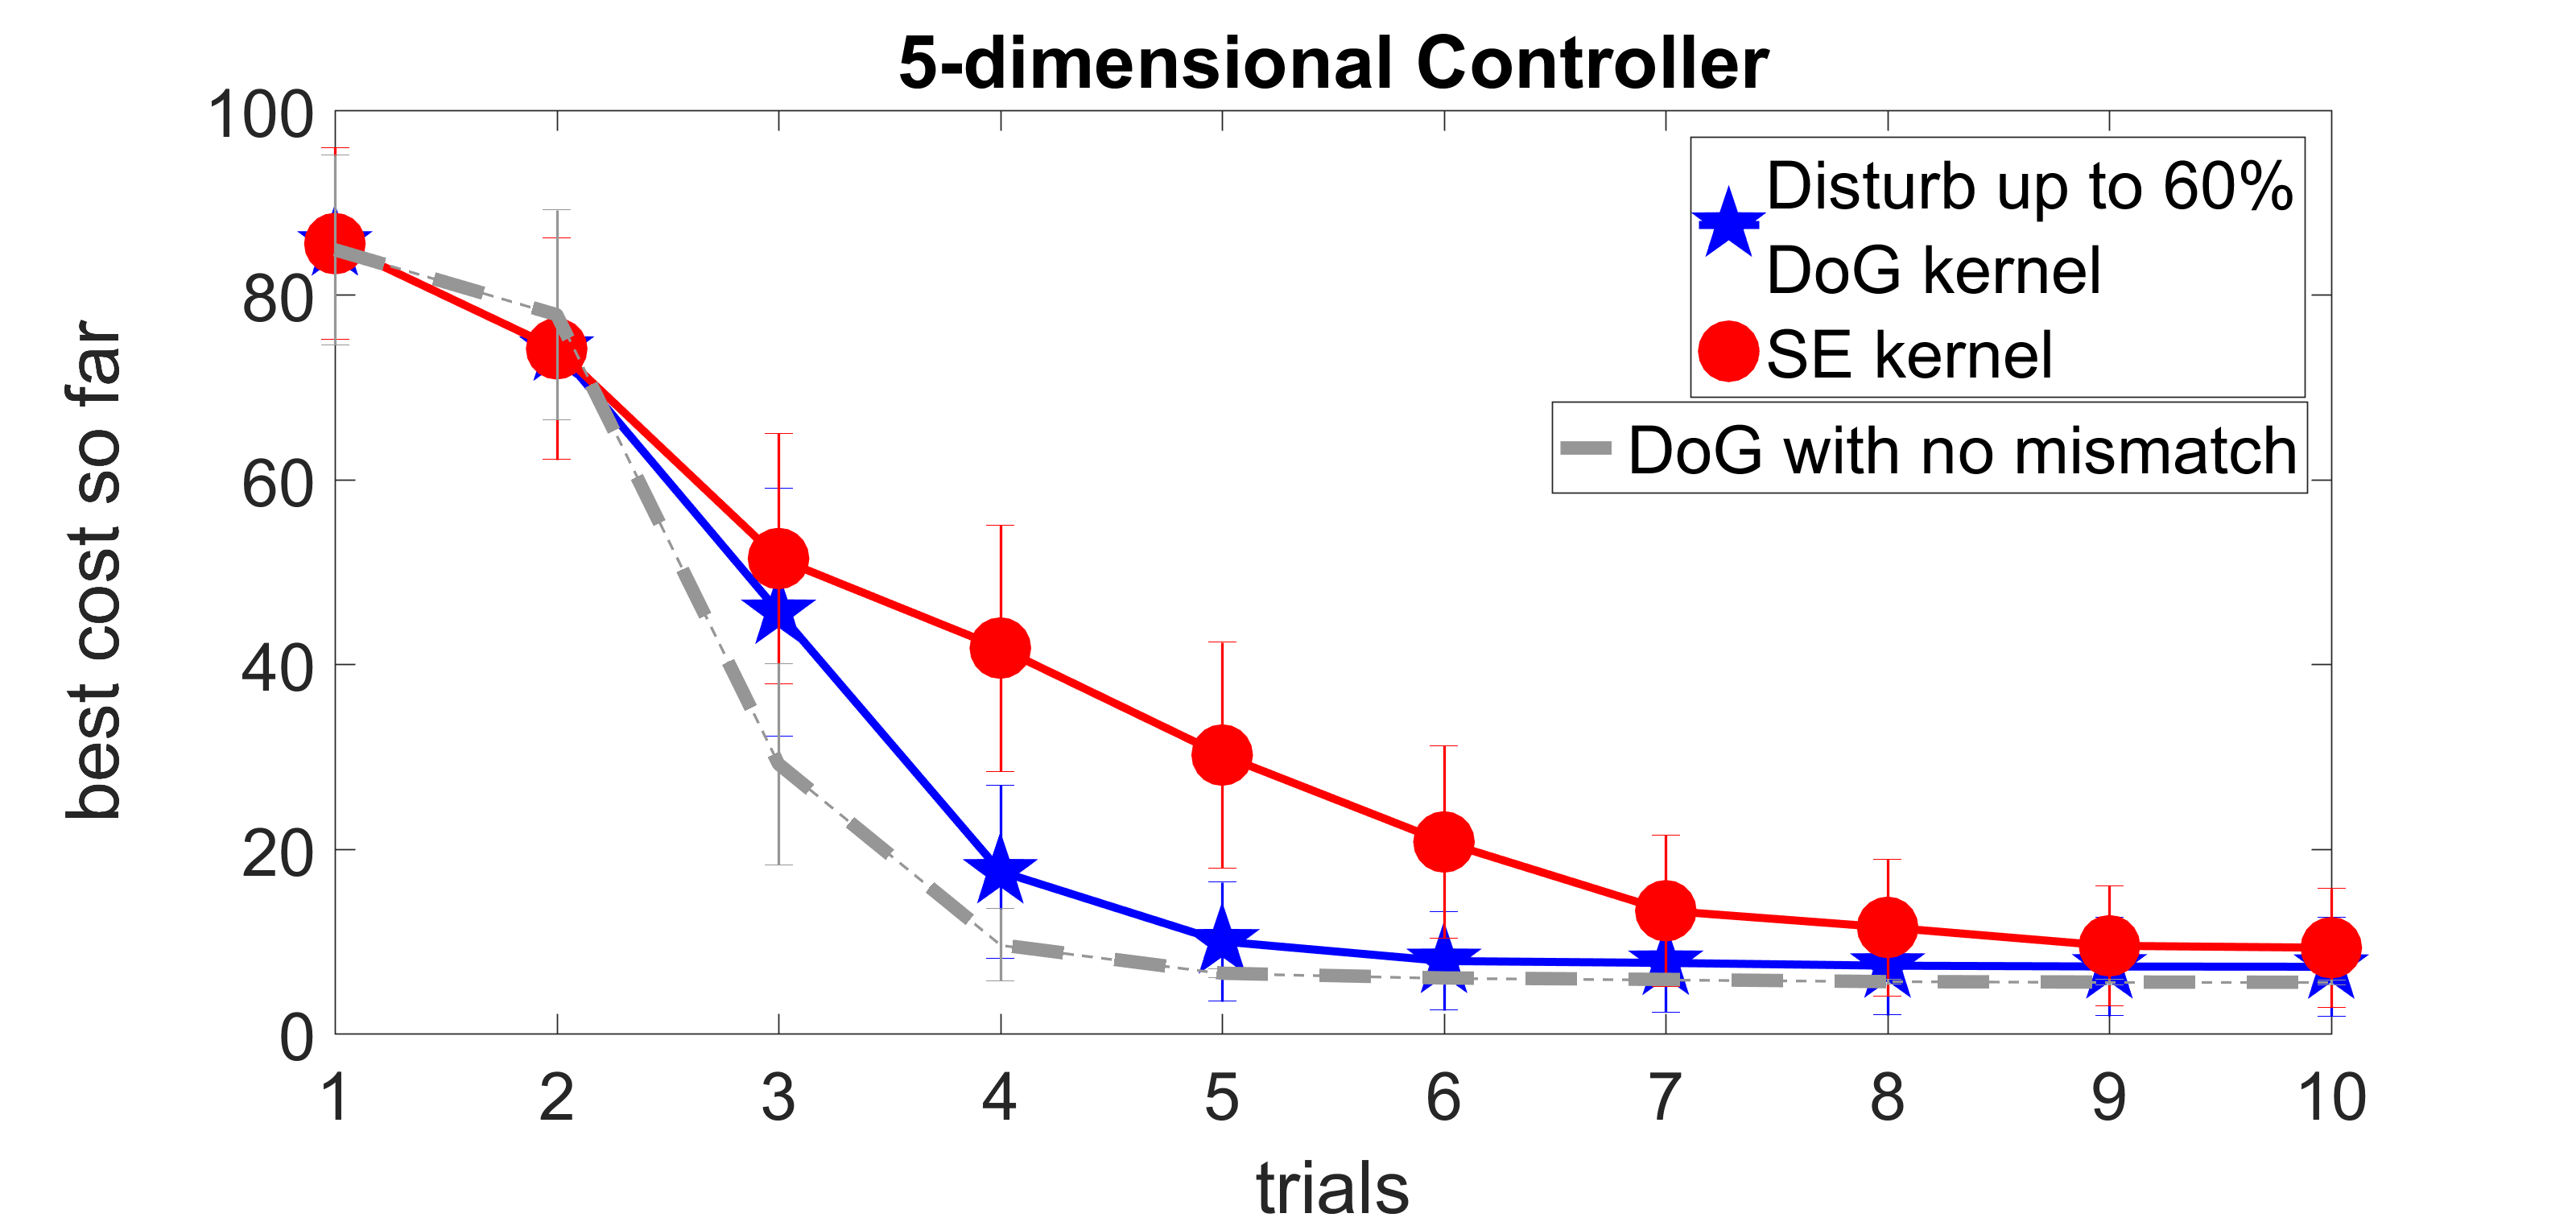
\includegraphics[width=0.65\textwidth]{img/BO_kernel_5d_disturb.png}
    \vspace{0.15cm}
    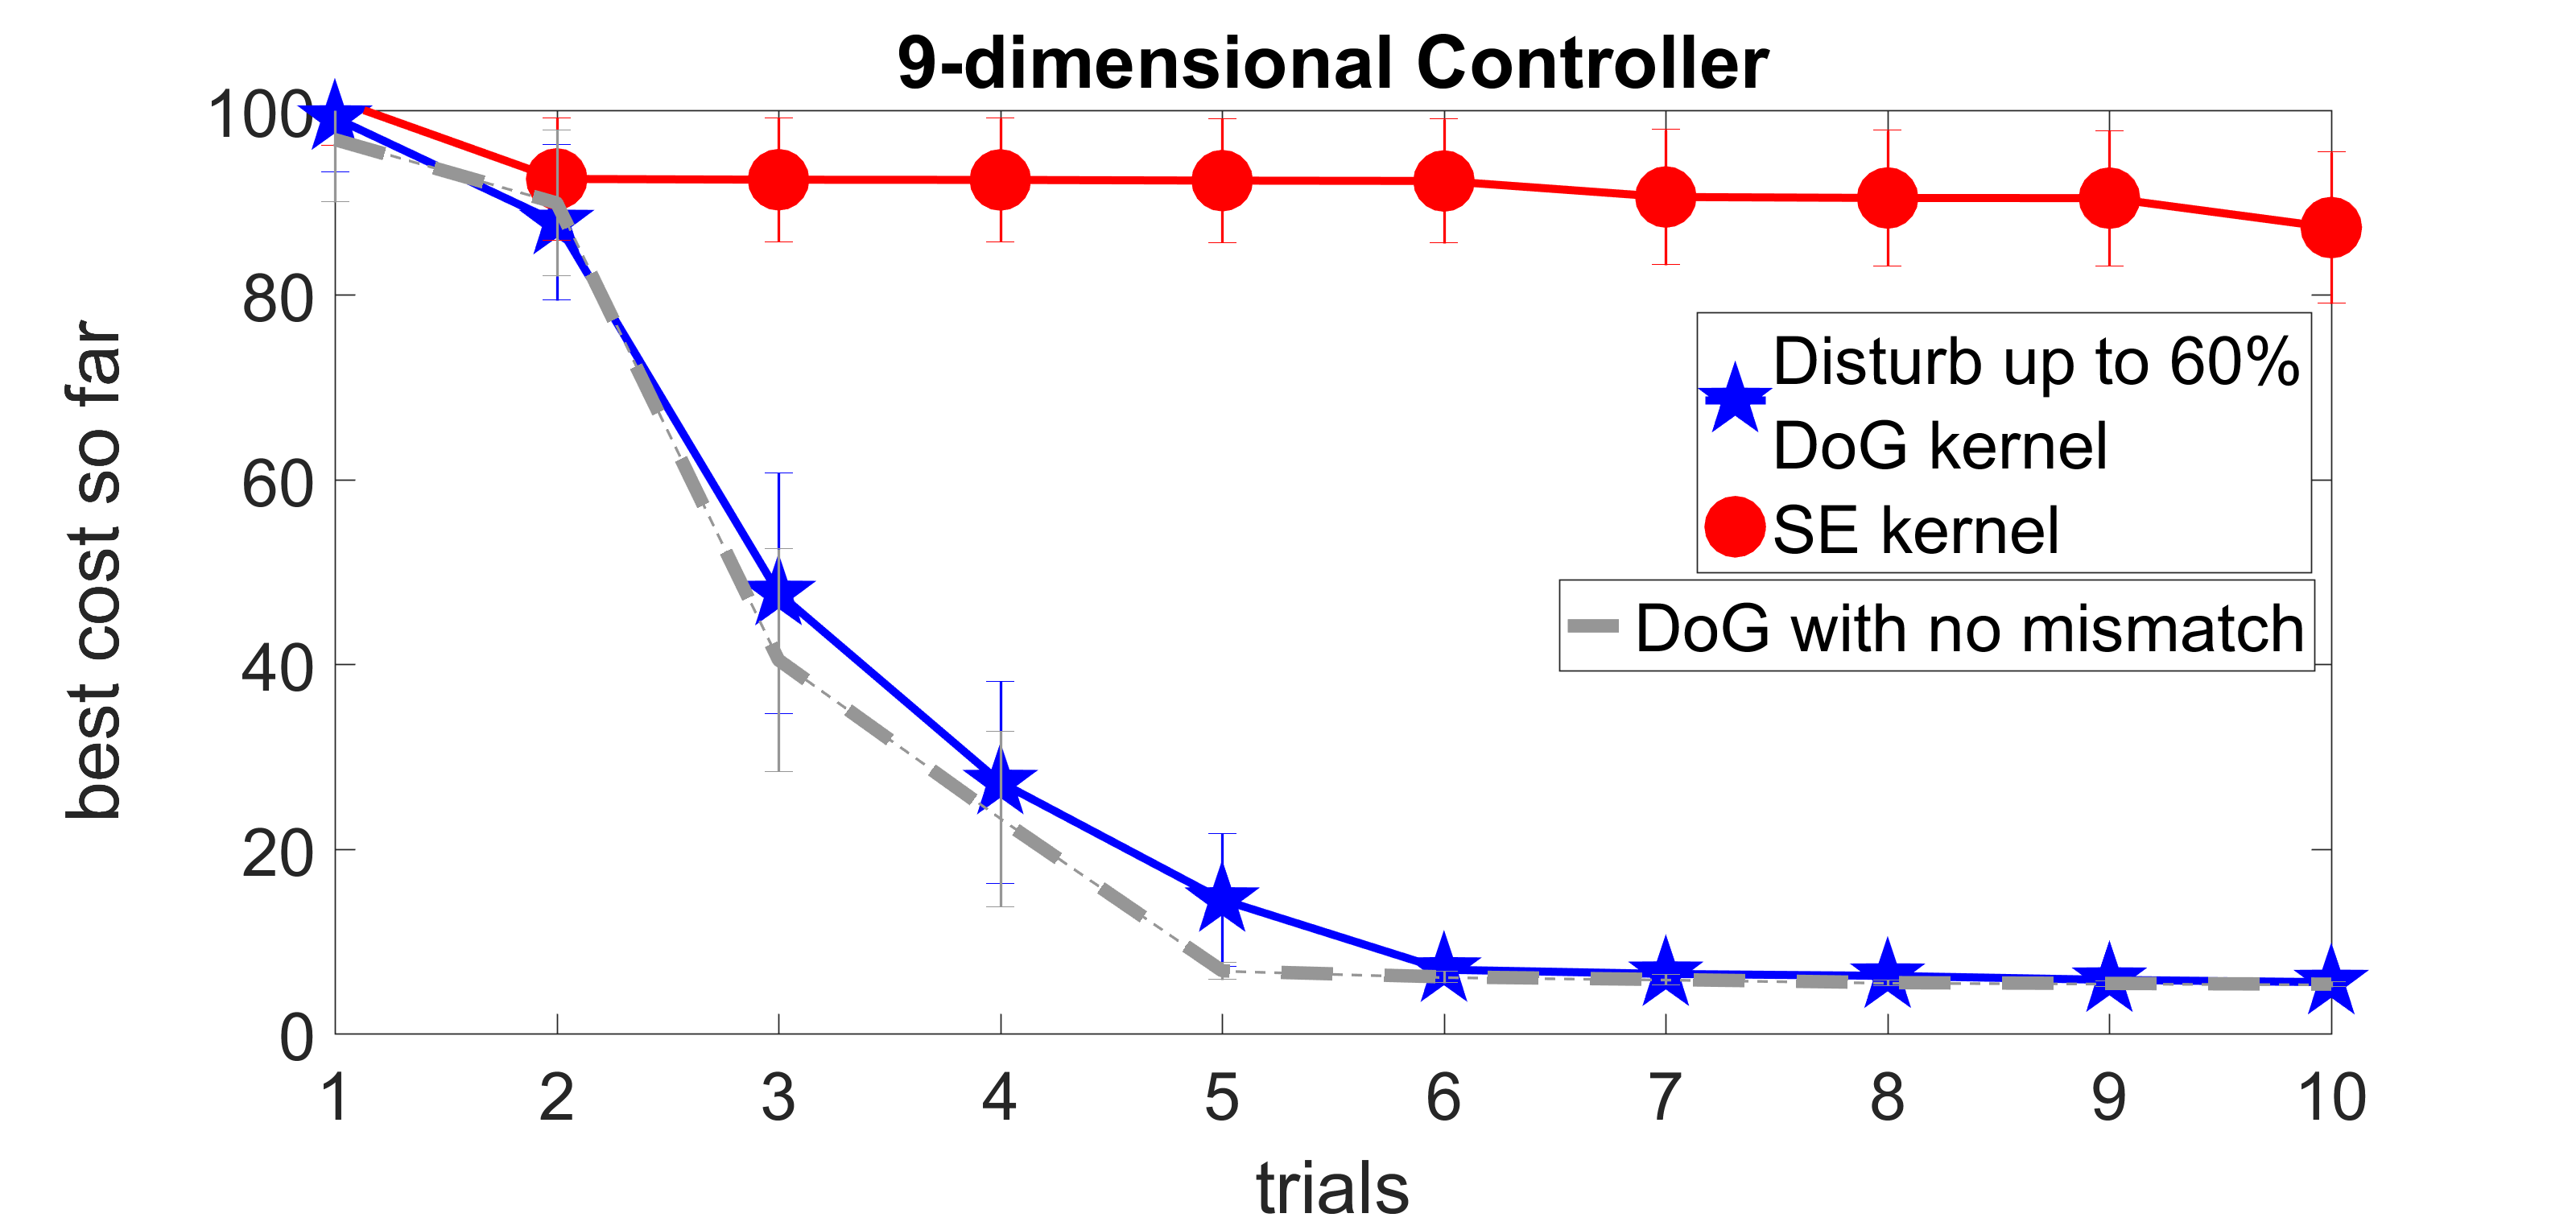
\includegraphics[width=0.65\textwidth]{img/BO_kernel_9d_disturb.png}
    \vspace{0.15cm}
    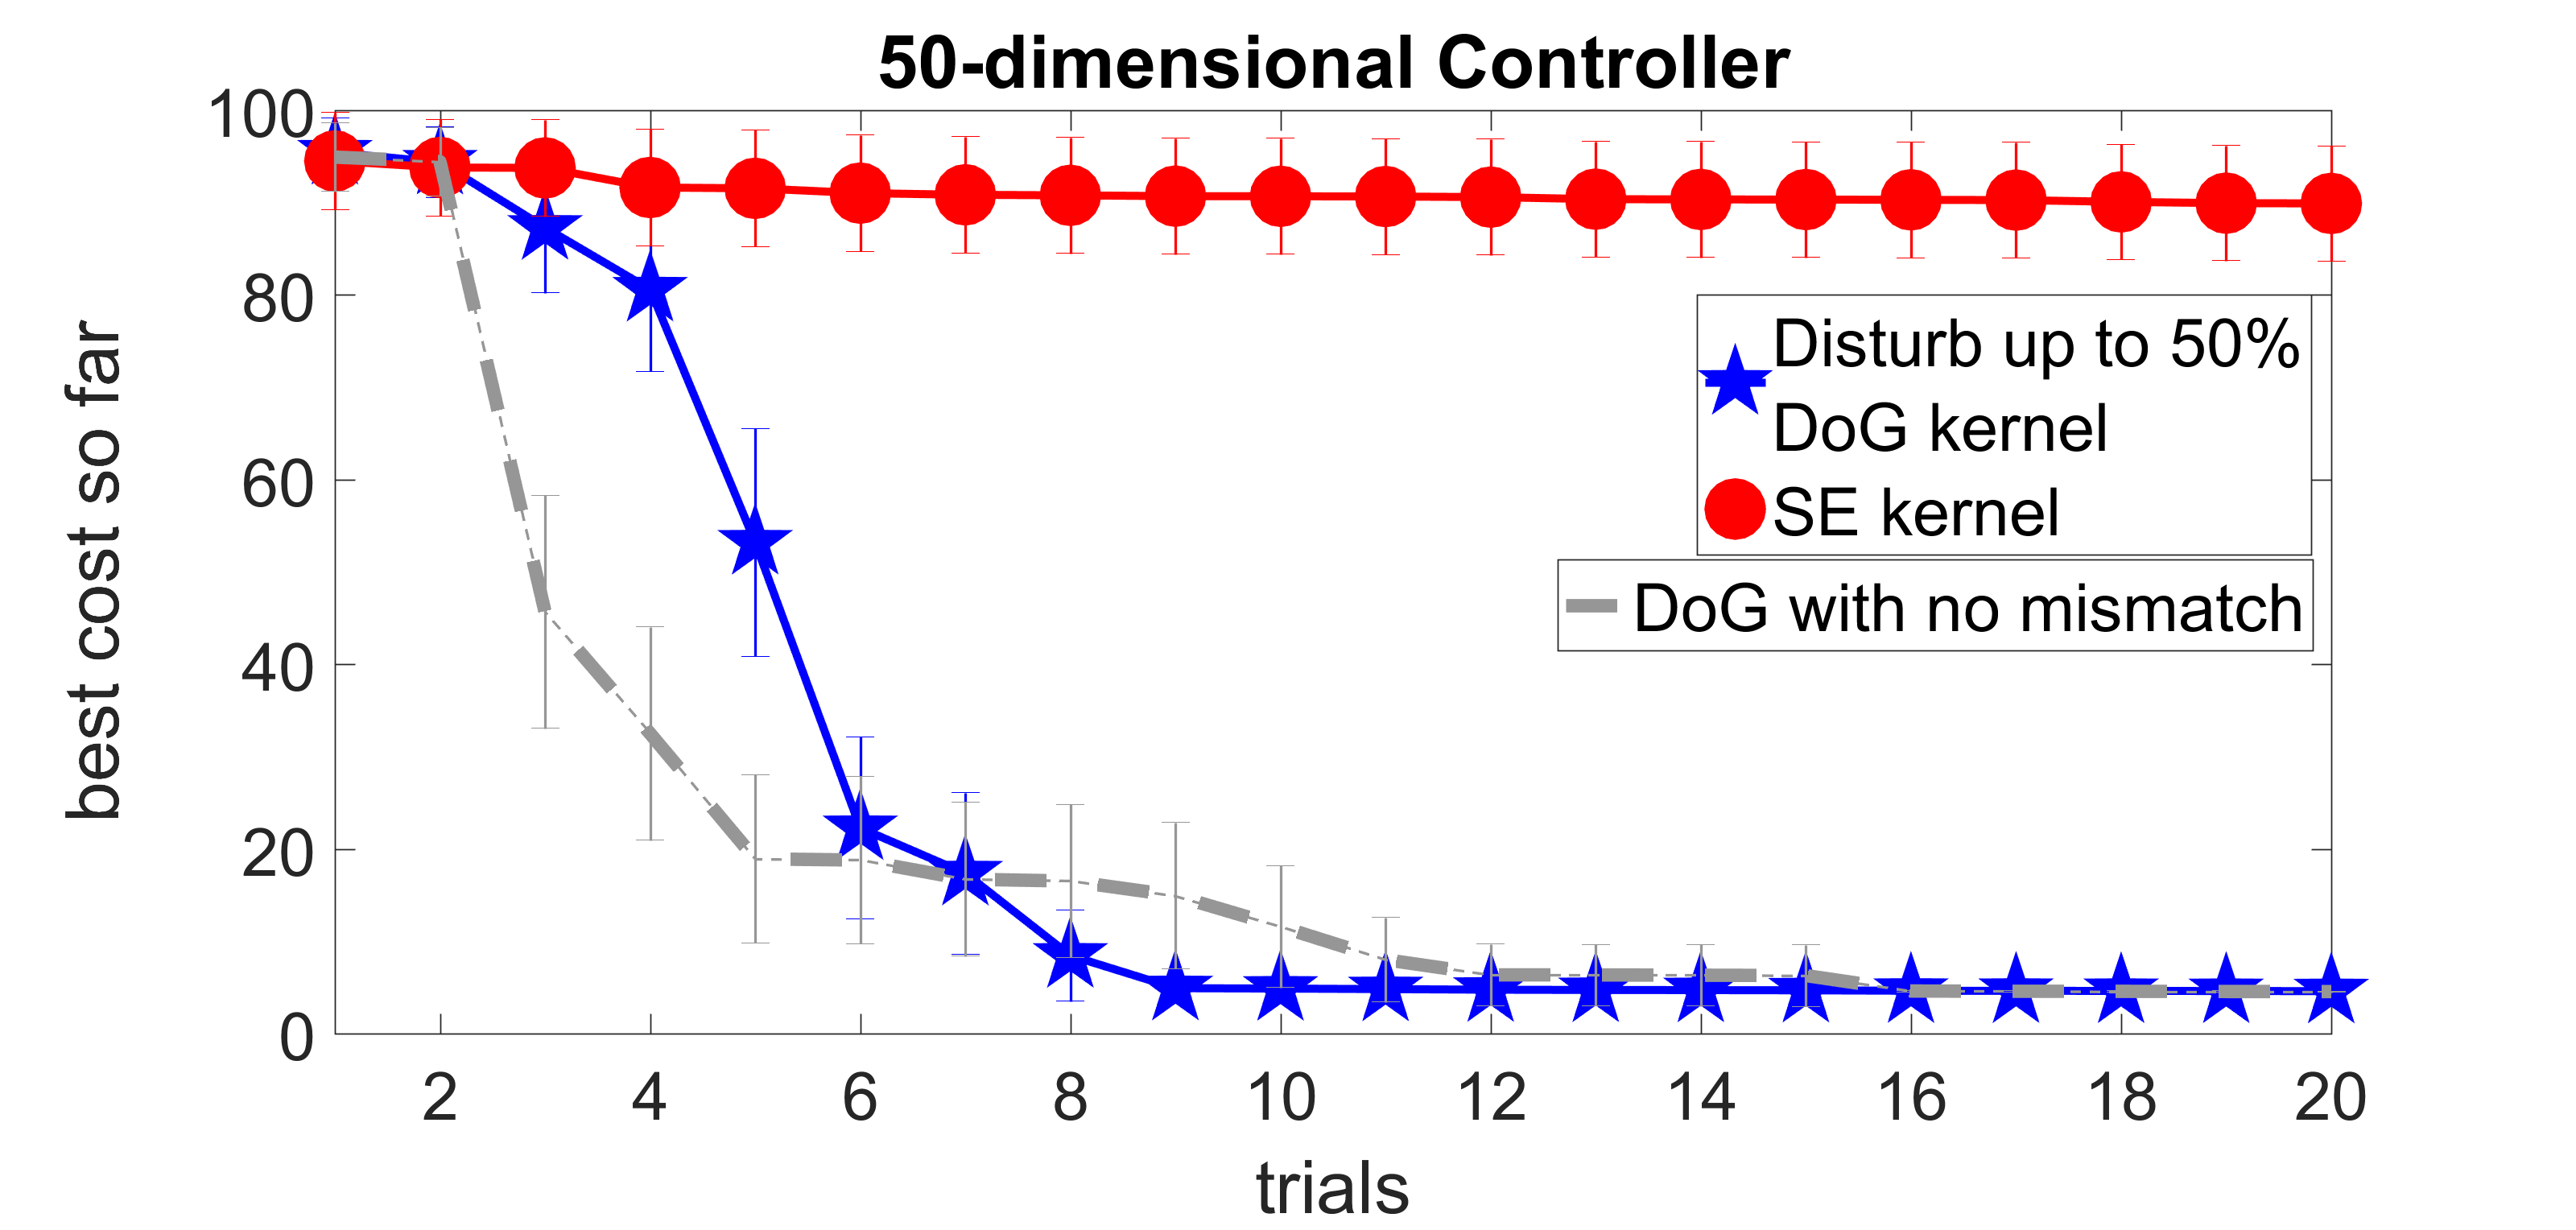
\includegraphics[width=0.65\textwidth]{img/BO_kernel_50d_disturb.png}
    \caption{Performance of DoG and SE kernel with disturbance for 5-dimensional (top), 9-dimensional (middle) and 50-dimensional (bottom) controllers over 50 runs. DoG with no simulation-hardware mismatch is also shown. DoG performs better than SE even on maximum disturbance, and performance does not deteriorate as disturbance increases.}
    \label{fig:dist_controllers}
\end{figure}

As shown in Figure \ref{fig:dist_controllers}, adjusted-DoG kernel obtains walking controllers in less than 10 trials for 5 and 9-dimensional controllers with up to $\pm$ 60\% perturbation of dynamics parameters. In comparison, while for the 5-dimensional controller BO with SE finds walking controllers in less than 10 trials, its performance deteriorates for the 9-dimensional controller. 
Our approach can scale well even to 50 dimensions, learning walking VNMC controllers reliably in less than 20 trials, with up to $\pm$ 50\% perturbation of dynamics parameters.

\AR{Add a summary of experiments in this section}



\chapter{Deep reinforcement learning for learning high level policies}

\label{chap:deep}

In this Chapter, we describe a second way of including simulation information in hardware experiments. Instead of building feature transforms in simulation, and learning controllers on hardware, we learn robust policies in simulation and implement them on hardware. We present our experiments on the effect of policy structure on rate of transfer between simulation and hardware.

\section{Neural network policies on the ATRIAS biped}

One way of transferring information between simulation and hardware is to directly learn a robust policy in simulation and deploy it on hardware. We train a deep neural network policy for controlling ATRIAS in simulation with ground height disturbance and test it on hardware. We experiment with different neural network controller structures, and study their effect on transfer from simulation to hardware, without any domain randomization. We show that structured neural network controllers have a fast training rate in simulation as well as higher rate of transfer to hardware. The structure also gives the user the power to modify the controller, if required, without having to re-train the neural network from scratch.

Deep reinforcement learning from scratch proved to be very challenging for a high-fidelity simulation of a bipedal robot. Deep RL methods depend on randomly exploring the space to get a notion of gradient of the cost. However, for underactuated bipedal robots most regions of space have very low reward, and hence no clear gradient. Stable walking regions in the controller space can be very narrow, making it unlikely to reach a promising controller by merely random sampling. To overcome this, we used behavior cloning to initialize our actor policy using the expert feedback-based reactive controller described in Section \ref{sec:raibert_cont}. Behavior cloning learns a policy over state-action pairs from expert trajectory by finding the policy parameters $\theta$ that solve the following maximum-likelihood optimization problem, as described in  \cite{rajeswaran2017learning}: 
\begin{equation}
    maximize_\theta \sum_{(s,a^*) \in \rho_D} ln \, \pi_\theta (a^*|s)
\end{equation}
where $\rho_D$ indicates the expert's trajectory distribution, with  $a^*$ is actions that expert took, and $s$ are the states visited.

Similarly, rewards accumulated during the expert's demonstrations can be used to pre-train a Q-function by minimizing TD error \citep{sendonaris2017learning}. As the Q-function provides the guidance for policy update, a well pre-trained Q-function benefits actor training as well. 

In practice, imitation learning does not guarantee that the cloned policy can work as well as the expert due to compounding error caused by distributional shift in states seen during training and testing, as described in  \cite{ross2010efficient}. Moreover, the expert controller might not perform sufficiently well in settings where it is difficult to design a controller. For example, while our expert controller is very stable on flat ground walking, rough ground seems to present a challenge. This means that the learned policy actually has to be updated to perform well in this situation, even in simulation. Nevertheless, the expert is a good initialization for the policy and makes the learning process much faster, by overcoming the need to randomly sample. We discuss two different types of neural network controllers that can be trained to obtain a better and more robust policy. 

\subsection{Neural Network Policy}
\label{NN_P}

In our first setting, we create a general neural network policy without a lot of structure. Similar to the expert controller, we design the action space of the neural network to be horizontal and vertical ground  reaction forces (GRFs) $F_z$, $F_x$ and the swing leg foot place location $x_p$. The input space is the state of the CoM:  (x,$v_{act}$,$z$,$\dot{z}$,$\theta$,$\dot{\theta}$). This means that the structure of the neural network policy becomes:
\begin{equation}
    \pi(x,v_{act},z,\dot{z},\theta,\dot{\theta})_{NN} \rightarrow  (F_z, F_x,x_p)
\end{equation}
The stance and swing control pipeline is similar to the expert and shown in Figure \ref{fig:NN_process}. The expert controller described in Section \ref{sec:raibert_cont} is used to pre-train the neural network policy to walk on flat ground.

\begin{figure}[!h]
	\centering
	\includegraphics[width=.7\textwidth]{./img/NN.PNG}
    \caption{Pipeline of our first neural network policy for controlling ATRIAS. Here $\tau_{RF},\tau_{RB},\tau_{LF},\tau_{LB}$ are torques in the right leg's front and back and left leg's front and back motors.}
    \label{fig:NN_process}
\end{figure}

While this policy still has the information about dynamics constraints of the robot through the inverse dynamics and inverse kinematics blocks, it loses the well-defined structure of the expert. This means that the output of the neural network is unpredictable, and the user does not have a lot of control over the behavior of the robot. Roboticists typically prefer controllers that can be understood and predictable, as well as can be modified if needed. In our second controller, we try to emulate this shared autonomy, which lets the user control the overall behavior of the robot, and the neural network helps improve the user-designed policy through deep reinforcement learning.

\subsection{Neural Network in the Heuristic Policy}\label{NN_HP}

In our second setting, instead of directly predicting the vertical and horizontal ground reaction force $ (F_z, F_x,x_p)$ as well as desired swing leg foot place location $x_p$, we use a neural network as part of the feedback based reactive stepping policy, described in Section \ref{sec:raibert_cont}. 
While the original policy has a fixed desired torso lean $\theta_{des}$, desired CoM height $z_{des}$ and fixed structure for $x_p$, we learn these as a function of the state of the CoM using a neural network. The neural network now takes the state of the CoM as input, and predicts the desired torso pitch, CoM height and an offset on the footstep location.
\begin{align}
  \pi(x,v_{act},z,\dot{z},\theta,\dot{\theta})_{HP} \rightarrow  (\theta_{NN}, z_{NN},x_{NN}) 
\end{align}

When inserted into the expert controller, this gives a structured neural network policy, where neural network outputs are used as part of a heuristic policy. It is worth noting that this policy is capable of generating the same outputs as the general neural network policy. For example, for any desired $F_{x}$ profile, it is always possible to find a $\theta_{NN}$ given $K_{pt}$, $K_{dt}$, $\theta$ and $\dot{\theta}$. The pipeline is illustrated in Figure \ref{fig:H_process}.

\begin{align}
F_x = K_{pt}(\theta_{NN} - \theta) + K_{dt}(-\dot{\theta}) \\
F_z = K_{pz}(z_{NN}-z) + K_{dz}( - \dot{z}) \\
x_p=k(v_{act}-v_{tgt}) + 0.5 \cdot v \cdot T + x_{NN}\label{x_p eq}
\end{align}


\begin{figure}[!h]
	\centering
	\includegraphics[width=.7\textwidth]{./img/Heuristic.PNG}
    \caption{Pipeline of our second neural network controller using a heuristic structure and neural network outputs for controlling ATRIAS. }
    \label{fig:H_process}
\end{figure}

There are several benefits to having such structure in our policies. First and foremost, the user can predict the behavior and understand the outputs of this policy. This is important for policies implemented on robots to ensure safety of the robot and its environment. 
%For example, controllers that use on inverse dynamics take torque constraints and other dynamics constraints into account. 
Moreover, if the user wants to test a slightly different setting than the simulation, she can easily tune other parameters of this policy, keeping the neural network fixed. Lastly, if the policy fails on hardware, it is easy for the user to understand why that might be, and even possible to fix other parts of the controller without re-training the neural network.


\section{Experiments with deep reinforcement learning}
In this section we describe our experiments with deep reinforcement learning for the ATRIAS bipedal robot. Our experiments compare a general neural network policy with a more structured policy, where the neural network helps modulate an expert controller. We compare both policies in simulation and hardware.

\subsection{Simulation Experiments}
%why doing simulation
We trained our neural network controllers in simulation before implementing on hardware. This is because we use Proximal Policy Optimization (PPO) as our learning algorithm. PPO needs to collect a large amount of data points at each iteration. When our current policy is not good enough, we would not be able to collect much data since the robot might fall at the very beginning of experiment. In order to collect enough number of data points, we need to do a large number of trials, making it near impossible to train on hardware. However, since we train our policies in simulation, the resulting controllers might work well in simulation environment but when implemented on hardware, they might fall. In order to overcome this issue, we add ground height disturbances to learn robust controllers in simulation. %Furthermore, while doing training, exploration can also be regarded as one kind of extra noise added to controllers.

\begin{figure}[t]
	\centering
	\includegraphics[width=.55\textwidth]{img/simulator.PNG}
    \caption{Simulation of ATRIAS with ground height disturbance. Different colors indicate different ground height disturbances. Maximum ground height disturbance is $\pm$ 10 cm. }
    \label{fig:process}
\end{figure}

The reward function is defined focusing on matching the desired walking speed and preventing large angular velocity of the torso. We also add a large penalty if the controller falls:
\begin{equation}
reward_t=\left\{
\begin{array}{rcl}
-C_1\cdot(v_{act, t}-v_{tgt})^2 -C_2\cdot(\dot{\theta}_t)^2 + 1 ,\  {if \ walk}\\
-C_3*T_{sim}, \  {if \ fall}
\end{array} \right.
\label{reward_1}
\end{equation}

where $v_{act, t}$ is the vector is the actual forward velocity of the robot at time $t$, $v_{tgt}$ is the target velocity, $\dot{\theta}_t$ is the angular velocity of torso pitch, $T_{sim}$ is the simulation time, $C_1,C_2,C_3$ are positive fixed parameters. This kind of cost function is similar to prior work on optimizing locomotion controllers, and it can easily distinguish points that walk from points that fall. The longer the controller can survive, the closer to the target speed, the less torso pitch the higher total reward the controller can get.
In this setting,$C_1 = 1$, $C_2=0.3$, $C_3=0.01$.
%One thing needs to be remarked is that the total reward does not directly indicate the robustness of the controller. For instance, a controller can overcome ground height disturbance might not have a high reward because it suffers from large penalty of large torso pitch which make the controller hard to be implemented on hardware. Anyway, the longer the controller can survive, the closer to the target speed, the less torso pitch the higher total reward the controller can get and more likely to work on hardware.
In our observation, often the highest scoring controllers in simulation tend to exploit simulation inaccuracies. For example, some controllers tend to jerk the torso to achieve speeds closer to the target speed. While these perform well in simulation, they tend to fail on hardware. 


%\TL{Explain the set up. How many data points per iteration? 3 runs of best controller? }%we also set our data collection number up to more than 3 full simulation episodes data, so if the controller fall in simulation, we would collect more episodes of data so that we can collect enough data in one iteration.

\subsubsection{Neural Network Policy}
The first set of simulation experiments were with the Neural Network Policy (NN Policy), described in Section \ref{NN_P}. The first step for Neural Network Policy was behavior cloning. After initialization, our NN policy could walk on flat ground, but it had difficulties with ground height disturbances. This was unsurprising because the 'expert controller' also cannot walk on ground with ground height disturbance. Hence, we had to train the policy further to achieve acceptable performance.
%More importantly, the 'expert controller' has a jump up behavior at the beginning of walking, and our initialization of NN policy also inherited this behavior. In simulation, this behavior would not lead to falling, but on hardware, ATRIAS would fall as soon as it tries to start walking because of the initial jump.

\begin{figure}[t]
	\centering
	\includegraphics[width=.55\textwidth]{./img/NN_walking.png}
    \caption{Sequence of frames from a single walking cycle (left to right). }
    \label{fig:NN_walking}
\end{figure}

%After initialization, we used DRL to improve the performance of our policy. 
We trained 10 different NN policies, the rewards for which are shown on Figure \ref{fig:Reward}. The rewards shown is the averaged reward of one iteration which consisted on 30,000 data points. %To reduce the influence of luck,  
As shown in the plot, the reward keeps growing as training goes on, starting from the average cost of the expert. This shows that PPO achieves a very stable training with little to no forgetting of the initial expert.

\begin{figure}[t]
	\centering
	\includegraphics[width=.65\textwidth]{img/NN_walking_2.png}
    \caption{A time lapse of Neural Network Policy walking around the boom with ground height disturbance in simulation. }
    \label{fig:NN_walking_2}
\end{figure}

\begin{figure}[t]
	\centering
	\includegraphics[width=.65\textwidth]{img/NN_H_reward.png}
    \caption{Training plot of Neural Network Policy (green) and Neural Network with Heuristic Policy (blue). Each of them is averaged of 5 trials data. In our training, we collected 30000 data in one iteration. For each simulation episode, we simulated 10 seconds if the controller keeps walking, and in simulation our time step was 0.001s. Thus, we could collect no more than 10000 data in a single episode, which also means in one iteration we needed data at least from 3 different episodes. By collecting data from more than one episodes, we could average the total rewards to determine the performance of the controller, also eliminating `lucky' runs.}
    \label{fig:Reward}
\end{figure}

\begin{figure}[t]
	\centering
	\includegraphics[width=.65\textwidth]{img/leg_force_profie.png}
    \caption{A plot of the stance leg SEA torques measured during one run of the NN policy on hardware. The torques are 0 during swing and follow a double hump pattern in stance. Note the high initial torques in the first two steps as compared to the rest of the walking cycle.}
    \label{fig:NN_walking_hw}
\end{figure}
The NN policy achieved good reward improvement compared to the initialization. After training, the NN policy could walk with ground height disturbance with a reasonable success rate. Figure \ref{fig:NN_walking} and Figure \ref{fig:NN_walking_2} shows the NN policy walking with ground height disturbance.


\subsubsection{Neural network with heuristic policy}

The second set of simulation experiment uses a neural network in a heuristic policy, described in section \ref{NN_HP}. %This heuristic policy don't have to do behavior cloning, we only initialized the outputs of Heuristic Policy to match the parameters of the 'expert controller'. 
By initializing this policy to the target values of the 'expert controller', the initial policy was able to walk on flat ground but cannot walk on rough ground. %And it still has a starting jump behavior.

The training plot of Heuristic Policy is shown on Figure \ref{fig:Reward}. As shown on the plot, the Heuristic Policy reward improves faster than the NN policy but reaches its peak in very few iterations. It then remains at that reward for the rest of iterations. The initial fast improvement is expected because as the heuristic policy uses the structure of the feedback-based reactive stepping policy, the search for reasonable parameters is simple. Hence, walking controllers are found much faster. However, the same structure also imposes a strong bias on the search, and as a result, it is hard to find controllers that can perform as well as the pure NN controller in simulation. However, as we describe later, even though the best reward achieved by Heuristic controllers is lower, the rate of transfer to hardware is much higher than the NN policy.

\begin{figure}[t]
	\centering
	\includegraphics[width=.85\textwidth]{img/Hardware.PNG}
    \caption{A time lapse of ATRIAS walking around the boom during a run of a NN with heuristic policy.}
    \label{fig:Hardware_walking}
\end{figure}

\subsection{Hardware Experiments}
\label{sec:nn_expts}
We tested 5 NN policies and 5 heuristic policies in our first set of hardware experiment, with the reward function described in Function \ref{reward_1}. 

There is a large mismatch between simulation and hardware starting conditions for our system. Starting from rest is a significant challenge for bipedal robots, especially underactuated robots like ATRIAS. ATRIAS is incapable of balancing by standing in place, and needs to continue stepping to stay upright. Typically, a start-up routine is designed for these robots to reach some initial walking gait, and then the controller to be tested is initiated. For example \cite{hubicki2016atrias} start by executing a stepping motion in air, and a human holds on to the robot as its lowered onto the ground. We train our controllers to start from rest in both simulation and hardware, to avoid having to design a start-up routine. However, our simulation leg is not initially loaded, so the simulation has to make an initial push to keep the CoM from going too low. On the other hand, on hardware the robot starts in position control in the air and then is lowered. So as stance starts, there is already sufficient force in the leg, and the initial push (from simulation) makes the robot leave ground. Such a controller falls on hardware. This behavior is illustrated in Figure \ref{fig:NN_walking_hw} where the first two steps on hardware experience higher leg forces than the rest of the steps.

\subsubsection{Neural network policy}

2 out of 5 of the NN policy could walk on hardware. But all of the NN policies shared the same issue that at the beginning of walking they would jump up. This behavior can also be seen in our simulation. The initializing 'expert controller' has a jump up behavior at the beginning of walking, and our NN policy also inherits this behavior. In simulation, this behavior would not lead to falling, but on hardware, ATRIAS would fall as soon as it tries to start walking because of the initial jump. On hardware, 2 out of 5 controllers could overcome the initial disturbance and then started normal walking pattern. 3 out 5 controllers, however could not recover from this disturbance. This led to a \textbf{$40\%$} rate of transfer of learned policies between simulation and hardware.

\subsubsection{Neural network with heuristic policy}

4 out 5 controllers trained with neural network as part of the heuristic structure were able to walk on hardware. There are a few reasons for the success of the NN with heuristic structure policy, over the pure NN policy. Firstly, the initial discrepancy between simulation and hardware leg force is already compensated for by the heuristic structure. In the simulation, the NN predicts a desired height, and the feedback on this desired height results in a high leg force, as the actual height of the robot is lower. On hardware, the actual height of the robot is close to this desired height, so it automatically reduces the initial leg force. Unlike pure NN policy, where the forces were high on both simulation and hardware, now the initial forces are only high when the actual state of the robot is different from the desired. This structure in our policy, hence, makes the generalization from simulation to hardware very simple and intuitive.

Secondly, since the structure of the policy is readable by an expert, the expert can still edit the policy after being trained in simulation. For example, if the NN was trained on a lower velocity but the expert wanted to run the robot on a higher velocity, the heuristic structure allows to directly edit this target. Similarly, we observed that some of our controllers were falling because of speeding, and we increased the feedback gain $k$ on velocity feedback, described in Equation \ref{x_p eq}. This modification significantly improved the success rate of policies learned in simulation on hardware.

These experiments highlight the advantages of structure in learned policies. While the NN helped us improve our heuristic policy, as shown in Figure \ref{fig:Reward}, by learning a state-dependant desired height, pitch and footstep location, it also kept the intuitive structure of the heuristic. So, it was able to better reject disturbances between simulation and hardware, as well as be modified for slightly different test situations, without needing re-learning. This allowed a \textbf{$80\%$} rate of transfer of learned policies between simulation and hardware.

\chapter{Conclusion}
\label{chap:conclusions}
%\AR{Add a big picture paragraph about learning on hardware.}

In this thesis, we presented different ways of adding simulation information to hardware experiments, with the aim of speeding up learning on hardware. We started with a global black-box optimizer like Bayesian Optimization, and added model-based information into it with the help of feature transforms. We studied different ways of designing these feature transforms, and compared their performance in simulation and hardware. Our results in Chapter \ref{chap:expts} show that our approach can learn controllers on hardware much faster than traditional optimization approaches like BO with SE kernel and CMA-ES on multiple robot morphologies and costs. 

Using simulation for hardware experiments raises the question of the effect of inaccuracies in simulation on the performance of the proposed approaches. To address this, we proposed a way of updating simulation models in a sample-efficient way in the space of features learned in the previous step. We then compared our approach and to approaches from literature on a series of increasingly inaccurate simulators -- with both inaccurate modelling parameters, as well as inaccurate dynamic models. Our experiments in Section \ref{subsec:mismatch_experiments} showed that while other approaches from literature might be able to learn faster with accurate simulators, our approach is more robust to simulation inaccuracies.

Lastly, we studied ways of training neural network policies in simulation and deploying them on hardware. While domain randomization is a popular approach for learning robust policies in simulation, it can lead to very conservative and low performance controllers. We experimented with the effect of structure in neural network policies learned in simulation on the rate of transfer to hardware. We trained two neural network policies on a simulation with ground height disturbances. The first policy was a general neural network with no expert-designed structure, while the second policy was part of a expert policy. Our experiments in Section \ref{sec:nn_expts} show that structured neural network policies can enhance the rate of transfer between simulation and hardware, as well as give the expert user control over the behavior to some extent. We think that this shared autonomy between the neural network and expert is highly desirable, as the neural network improves the expert policy while benefiting from the knowledge of the expert.

In this chapter, we discuss each section of this thesis in some detail, provide some limitations and future directions. We finish by discussing some open questions in learning for robotics, and the application of the work done in this thesis to such questions.


\section{Discussion}
This thesis covered three main ideas : (1) Incorporating simulation information in hardware experiments with the help of feature transforms. (2) Updating these transforms to account for simulation inaccuracies. (3) The use of structure in high-dimensional neural network policies learned in simulation. 
We discuss each of these ideas in some detail next.

\subsection{Feature transforms from simulation in hardware experiments}

Adding simulation information to hardware experiments is well explored in literature. For example, \cite{endo2008learning} learn a policy in simulation and then continue gradient descent on hardware to further optimize the policy. It is also common to hand-tune controllers learned in simulation by an expert.  \cite{abbeel2006using} use learn an inaccurate model of the dynamics from simulation, and continue to improve it from data on hardware. While these approaches are promising when we expect our simulation to be close to hardware, they can be very expensive in terms of number of samples if the simulation is very inaccurate. The bias from simulation can get local optimizers stuck in bad local minima, and it might be difficult or impossible to recover, as demonstrated in Section \ref{subsec:sim_experiments_prior_cully}.

We design a way of incorporating simulation information in a global sample-efficient optimizer on hardware. Instead of adding simulation information to the prior, we add information about simulation trajectories to the kernel. This means that hardware experiments are now guided by the controller behavior recorded in simulation. This transforms the original controller space into a lower dimensional, easier to learn space, where controllers likely to perform well on hardware are close together, and far away from those that are likely to perform poorly.

This lower-dimensional feature space can be hand-designed, in cases where expert knowledge about the task is available. For bipedal locomotion, we describe such features in Section \ref{sec:dog_transform}. On the other hand, raw trajectories, or trajectory summaries from simulation can also be used to create a higher-dimensional but informed feature space. We do this by training a neural network to predict simulation trajectories, as described in Section \ref{sec:approach_traj}. Our hardware experiments on ATRIAS show that both these approaches are able to learn walking controllers very sample-efficiently. They significantly outperform uninformed BO and random sampling. Simulation experiments on a 7-link-biped in Section \ref{sec:7_link_expts} show that these generalize to multiple robot morphologies and controller types.

These experiments showed that features learned in a high-fidelity simulation were able to help improve sample-efficiency of Bayesian optimization during hardware experiments. While domain-informed kernels performed slightly better than the neural network kernels, both learned a 9-dimensional walking controller in less than 10 trials. For a 50-dimensional controller, we showed improvement in simulation. These controllers are still low dimensional as compared to high-dimensional controllers like neural networks. 
In the future, we would like to study if such features can be developed for very high-dimensional policies, possibly enabling these to be directly learned on hardware. 

\subsection{Accounting for simulation inaccuracies}

An important question that arises when using simulation for learning on hardware is : how does performance deteriorate if the simulator is bad? While there are a lot of ways of incorporating simulation information in hardware experiments, there is not a lot of research on studying the effect of inaccurate simulations on these approaches. We develop a systematic way of studying the effect of increasing inaccuracies on the performance of our proposed approach, and compare it to other approaches in literature.

We first study the effect of inaccurate modelling parameters, such as mass, inertia, length and center of mass of each link. These parameters can also be typically identified with system-identification approaches as described in \cite{An:1988:MCR:47324}. However, parameters like friction coefficients and sensor and actuator delay can be variable over experiments, and would need to be re-identified continually. Thus, some amount of robustness to changes in these parameters is ideal. We collect features in an unperturbed simulation, and study optimization performance in \textit{simulated hardware} with up to $\pm50\%$ perturbed inertial parameters. Next, we studied the effect of incorrectly modelled dynamics, such as simplified actuator dynamics and incorrect boom model on the performance of different approaches that transfer information from simulation to hardware. Unmodelled dynamics form a major part of real robot simulators and can be challenging to overcome. In our setting, the high-fidelity original simulator serves as the test model and low-fidelity simulators serve as the source of training data. It is worth noting that the difference between simulation and hardware is not known during test time.

To account for the mismatch between simulation and hardware, we measure the difference between simulation and hardware features, and build a mismatch model from this data. This model lets up update the simulation features in a sample-efficient manner, helping build a better representation of the hardware. Our experiments show that disturbances due to incorrect inertial parameters are in fact easy to overcome with such an update scheme. Features from perturbed simulations find walking controllers in less than 10 trials. On the other hand, inaccurate dynamics models are much harder to compensate for, taking up to 50 trials to learn walking controllers reliably. While other approaches from the literature, like \cite{cully2015robots} can do well when the simulation is close to hardware, they fail to find walking controllers reliably in the presence of large mismatch between simulation and hardware (Figure \ref{fig:cully_prior_sim_versions}). On the other hand adjusted \dogkernel can learn to walk even with large simulation inaccuracies, though it might be less sample-efficient when the simulation is accurate.

Our experiments demonstrated the advantages and disadvantages of using simulation information during hardware experiments. While most approaches are highly sample-efficient when simulation is close to hardware, they suffer when the two are significantly different. This is expected, as the information from simulation is not accurate anymore and the performance of simulation-informed BO can be worse than uninformed BO. On the other hand, adjusted \dogkernel is able to recover from the simulation inaccuracy and guide the search to a region reliable on hardware. Conversely, the adjusted \dogkernel is also less sample-efficient than other approaches when simulation is very close to hardware, as it spends some samples trying to learn about the function and mismatch landscape.

While our evaluations focused on locomotion, the need for incorporating simulation robustly is profound in other of parts robotics, particularly manipulation. Successful modeling of contact dynamics in manipulation is challenging, even for known object/surface types. Utilizing simulation for complex and dynamic manipulation tasks can be useful, since such simulation could be informative in some parts of optimization space, but incorrect in other parts. 
We hope that our experimental setup can be used for analyzing the effectiveness of methods at handling simulation-hardware mismatch in domains other than locomotion, and approaches we evaluate can be adapted to work in other parts of robotics.



\subsection{Effect of structure on high-dimensional neural network policies}

Recently, there has been a lot of interest in learning very high-dimensional neural network policies in simulation using deep reinforcement learning, for example \cite{rajeswaran2017towards}, \cite{peng2017sim}, etc. To transfer these policies to hardware, a common approach is to learn robust policies with the help of domain randomization, as in \cite{mordatch2015ensemble}, \cite{tan2018sim}. These works aim to 
learn robust policies by considering a distribution of model parameters in simulations, which includes the real model of the robot. While this is a very effective way of learning policies that transfer between simulation and hardware, the performance of learned policies is typically poorer than policies learned without domain randomization \citep{tan2018sim}. In our work, we take a different approach to transferability of controllers. Instead of using domain randomization, we explore how structured controllers can eliminate the need to use domain randomization, and lead to a high rate of transfer of policies between simulation and hardware.

We train two neural network policies in simulation - a general NN policy that directly predicts desired forces, and a structured NN policy that predicts set points of a expert-designed policy. Both NN policies are capable of generating arbitrary forces, so there is no loss in generalization with the structure. Our experiments suggest that the structured policy has a much higher rate of transfer between simulation and hardware. Additionally, the structure of the policy lets the user edit the policy for a new, but related, task without retraining the network. This enables a shared autonomy between the NN and the expert, where each benefit from the other.

\cite{peng2017learning} have shown that even in simulation the choice of action space affects the rate of learning as well as disturbance rejection. Building on this, we study the effect of action space, and in particular, the structure of the NN policy on transfer between simulation and hardware. Unsurprisingly, NN policies with an expert-designed structure are able to generalize to unseen state distributions better than a general NN policy without any structure. For example, in most bipedal robots, the initial conditions between simulation and hardware are quite different. The structured NN policy was able to overcome this disturbance and continue walking at the desired speed. On the other hand, the NN policy without structure was not able to handle this case reliably, and failed to walk. Our experiments show that it is indeed possible to learn high-performing policies in simulation that can transfer to hardware without using domain randomization. Expert-designed structured policies are beneficial for two reasons. The NN helps improve the performance of hand-designed heuristics. In addition, the structure enables the user to predict and change the behavior of the NN policy without retraining. 

\section{Future work and open questions}

There are several extensions to the current work, as well as unanswered questions about learning for robotics.

\subsection{Learning general features from data}

We presented two sets of feature transforms for adding simulation information to hardware experiments. So far, the features were either hand-designed or needed expert input in the relevant simulation trajectories. Very often, there were iterations needed where the right features were not selected, or too many features were selected, bringing down the sample-efficiency. Thus, it is important to explore if such features can be learned directly from data, and important characteristics dynamically added or removed based on the problem at hand. 

Features should also include feedback from the environment, for example contact forces. Other than just the end-effector trajectory, the instantaneous forces can also be indicative of the success or failure of particular controllers. Learning low-dimensional representations of these feedback trajectories is an interesting direction for future work. 

Adapting features across multiple tasks and changing lower dimensional representations with context, can be useful for transferring data between different tasks and robots. This requires a sample-efficient way of updating features based on newly observed hardware samples, along with automatically determining the relative importance of features. All of these can together be used to build task-specific lower-dimensional representations that can be learned dynamically, and used to transfer information across multiple tasks.


\subsection{Safe exploration and learning}

A major concern with learning for robots is the safety of the robot. Exploration often involves sampling controllers that could potentially be unstable and damage our robots. Even worse, robots can damage their surroundings, including people and objects that they interact with. Taking safety of a robot and its environment into account is important when using approaches like Bayesian optimization and reinforcement learning.

\cite{berkenkamp2017safe} develop guarantees for model-based reinforcement learning when the dynamics are approximated as a Gaussian process. The policies sampled are guaranteed to be in the region of attraction of an initial stable policy. This is an important step in the direction of building guarantees about safety, but stable initial policies can be hard to find in high-dimensional systems. Building dynamics models might also be prohibitively expensive, and it may be nearly impossible to make them accurate. In such cases, detecting failure or a mismatch between expectation and measurement becomes important. 

We think that starting with conservative policies learned in simulation and slowly building dynamics models is an interesting direction to explore in the future. Exploration while learning dynamics can be done with the help of conservative models and controllers, that build failure maps from expected and measured sensor feedback. All of this together can bring us closer to truly autonomous robots that learn to accomplish goals, starting from inaccurate models and conservative controllers, and slowly learning better controllers along with the dynamics.

\subsection{Transfer learning between controllers}

Given how expensive reinforcement learning typically is, it is important to learn systems that can share information and data. Transfer learning is a popular research direction, with works like \cite{finn2017one} trying to identify task-parameters and learn networks that generalize across multiple tasks. While this is promising, compelling hardware demonstrations of these approaches are few. We believe that automatic relevance determination between task-specific features can be an important step towards transfer learning and data sharing. Different tasks can have different important features, and a correspondingly different cost function. But data from the previous task can be included as if from a different source, as in \cite{poloczek2016multi}. 

In addition, learning problem representations that can generalize across multiple robots can allow for
data transfer across multiple robots. Sharing data in this manner can be extremely helpful in learning to do new tasks sample-efficiently. 

\section{Closing remarks}

This thesis tried to address the problem of fast learning in highly dynamic systems, with the help of simulation. We found that even when the simulator is inaccurate, information from simulation can guide hardware experiments to improve sample-efficiency. We also showed that learning lower-dimensional representations of the controller space in simulation not only helps learn faster on hardware, but also enables us to update the simulation in the same space. 

All of this points towards the advantages of learning representations for optimization and learning. We believe that there are additional advantages to learning representations, like failure detection, safety and transfer learning. We would like to continue exploring these directions in the future.

%----------------------------------------------------------------------------------------
%	THESIS CONTENT - APPENDICES
%----------------------------------------------------------------------------------------

\appendix % Cue to tell LaTeX that the following "chapters" are Appendices

% Include the appendices of the thesis as separate files from the Appendices folder
% Uncomment the lines as you write the Appendices

%% Appendix A

\chapter{Frequently Asked Questions} % Main appendix title

\label{AppendixA} % For referencing this appendix elsewhere, use \ref{AppendixA}

\section{How do I change the colors of links?}

The color of links can be changed to your liking using:

{\small\verb!\hypersetup{urlcolor=red}!}, or

{\small\verb!\hypersetup{citecolor=green}!}, or

{\small\verb!\hypersetup{allcolor=blue}!}.

\noindent If you want to completely hide the links, you can use:

{\small\verb!\hypersetup{allcolors=.}!}, or even better: 

{\small\verb!\hypersetup{hidelinks}!}.

\noindent If you want to have obvious links in the PDF but not the printed text, use:

{\small\verb!\hypersetup{colorlinks=false}!}.

%\include{Appendices/AppendixB}
%\include{Appendices/AppendixC}

%----------------------------------------------------------------------------------------
%	BIBLIOGRAPHY
%----------------------------------------------------------------------------------------

\printbibliography[heading=bibintoc]

%----------------------------------------------------------------------------------------

\end{document}  
